\documentclass[12pt]{report}
\usepackage{vmargin}
\setpapersize{A4}
\setmargins{2.5cm}       % margen izquierdo
{2.5cm}                  % margen superior
{16.5cm}                 % anchura del texto
{23.42cm}                % altura del texto
{10pt}                   % altura de los encabezados
{1cm}                    % espacio entre el texto y los encabezados
{0pt}                    % altura del pie de página
{2cm}                    % espacio entre el texto y el pie de página

\usepackage[spanish,es-tabla]{babel} % Idioma español con tablas
\usepackage{longtable}     			 % Usado para diseñar grandes tablas.
\usepackage{multirow} 				 % para las tablas

\usepackage{amsmath, amssymb, amsfonts, latexsym, anyfontsize}
\usepackage{color, alltt, times}
\setcounter{secnumdepth}{3} % Para que ponga 1.1.1.1 en subsubsecciones
\setcounter{tocdepth}{3}    % Para que ponga subsubsecciones en el indice
\usepackage{setspace}       % Usado para %\onehalfspace  \doublespacing  \singlespace
\usepackage{booktabs}       % Para formar tablas
\usepackage{appendix}       % Para los anexos
\usepackage{url}            % Para citar las urls
\usepackage{pdfpages}       % Para insertar documentos de tipo PDF
\usepackage{epstopdf}       % Para insertar imagenes en formato eps obtenidas en Matlab
\usepackage{graphicx}       % Para las imagenes y gráficos
\usepackage{subfigure}      % Para subfiguras

\usepackage[utf8]{inputenc} % Para escribir en castellano
\usepackage[T1]{fontenc}

\usepackage{algorithmic}
\usepackage{algorithm}

\usepackage[x11names,table]{xcolor}
\usepackage{caption}
\usepackage[round]{natbib}
 
\begin{document}
\baselineskip 1cm
\pagestyle{plain}
%%%%%%%%%%%%%%%%%%%%%%%%%%%%% CARATULA%%%%%%%%%%%%%%%%%%%%%%%%
\textheight 19cm
\pagestyle{empty}
\begin{center}
 {\bf {\fontsize{14}{16.8}\selectfont UNIVERSIDAD NACIONAL DE TRUJILLO}}     
 
    {\bf{\fontsize{14}{16.8}\selectfont Facultad de Ciencias Físicas y Matemáticas}} 

  {\bf{\fontsize{14}{16.8}\selectfont Escuela Profesional de Informática}}
\end{center}  

\begin{figure}[ht]
\begin{center}

\includegraphics[width=.4\textwidth]{Imagenes/Cap0/unt}
\end{center}
\end{figure}
\vskip 0.5cm

\begin{center}  
    {\bf\Large{{\fontsize{17}{20.4}\selectfont{} Sistema de seguridad para el control de acceso a una vivienda mediante el reconocimiento de voz utilizando coeficientes cepstrum MFCC Y DTW}}}
\end{center}   

\begin{center}
{\Large{TESIS}}
\end{center}
\begin{center}
{\large{\hspace*{0.4cm} PARA OPTAR EL TÍTULO PROFESIONAL DE INGENIERO  INFORMÁTICO}}
\end{center}

\vskip 0.6cm
\begin{center}
  { \fontsize{14}{16.8}\selectfont {\hspace{-2.9cm}AUTORES: Ocas Quiroz Carlos E.}} \\
    { \fontsize{14}{16.8}\selectfont {\hspace{-0.4cm} Sánchez Pedro Edwin J.}}\\
    \vskip 0.2cm
    { \fontsize{14}{16.8}\selectfont {\hspace{-1.7cm} ASESOR: Ms. Peralta Luján José L.}}
\end{center}  

\vskip 1.1cm
\begin{center}    
{\bf {\fontsize{14}{16.8}\selectfont TRUJILLO - PERÚ
\vskip 0.0cm
\hspace*{-0.2cm} 
2019 }}
\end{center} 
\newpage
%%%%%%%%%%%%%%%%%%%%%%%%%%%%%%%%%%%%%%%%%%%%%%%%%%%%%%%%%%%%%%%%%%%%%%%%%%%


%%%%%%%%%%%%%%%%%%%%%%%%%%%% DEDICATORIA %%%%%%%%%%%%%%%%%%%%%%
 \pagestyle{plain}
 \pagenumbering{roman}
 \addcontentsline{toc}{chapter}{Dedicatoria}
 {\bf\Large {Dedicamos esta tesis a :}}
 \vskip 1cm
\begin{quotation}
{\it Nuestras familias por el apoyo incondicional y permanente que nos brindaron durante nuestra preparación académica para poder llegar a ser profesionales competitivos y de éxito, quienes con su amor y paciencia permitieron cumplir un deseo tan esperado, y que ahora permite ser útil a nuestro país.}
\end{quotation}
%%%%%%%%%%%%%%%%%%%%%%%%%%%%%%%%%%%%%%%%%%%%%%%%%%%%%%%%%%%%%%%%%%%%%%%%%%%


%%%%%%%%%%%%%%%%%%%%%%%%%%%% AGRADECIMENTOS %%%%%%%%%%%%%%%%%%%%%%
\newpage

 \addcontentsline{toc}{chapter}{Agradecimientos}
 {\bf\Large {\flushleft{Agradecimientos}}}
\vskip 0.2cm
\begin{quotation}
A Dios y a nuestros padres, ya que sin ellos nada de esto hubiera sido posible.
{\vskip 0.2cm}
A nuestro asesor de tesis, Ms. José Peralta Luján, que, con su amistad, apoyo, paciencia, dedicación, consejos y observaciones en la realización de este trabajo pudimos sacar adelante esta tesis y además por darnos las herramientas necesarias para ser mejores profesionales cada día.
\vskip 0.2cm
Al Ing. Clayder Gonzales Cadenillas, que desde un principio se mostró siempre disponible e interesado, brindándonos su apoyo y motivándonos en esta área de investigación.
\vskip 0.2cm
A nuestros amigos, Ing. Javier Fuentes Huertas e Ing. Alexis Aspauza Lezcano, por el apoyo y consejos dados como extesistas en la carrera de Informática.
\vskip 0.2cm
Al Dr. Jorge Guevara Días, por el apoyo y sus excelentes comentarios brindados en mejora de la investigación.
\vskip 0.2cm
Al honorable jurado, por sus valiosas aportaciones.
\vskip 0.2cm
A la Universidad Nacional de Trujillo, por la formación que en ella recibimos y a nuestros profesores por habernos brindado parte de su sabiduría y amistad.
 \end{quotation}
%%%%%%%%%%%%%%%%%%%%%%%%%%%%%%%%%%%%%%%%%%%%%%%%%%%%%%%%%%%%%%%%%%%%%%%%%%%


%%%%%%%%%%%%%%%%%%%%   ACTA SUSTENTACION   %%%%%%%%%%%%%%%%%%%%%%%%
%\setboolean{@twoside}{false}
%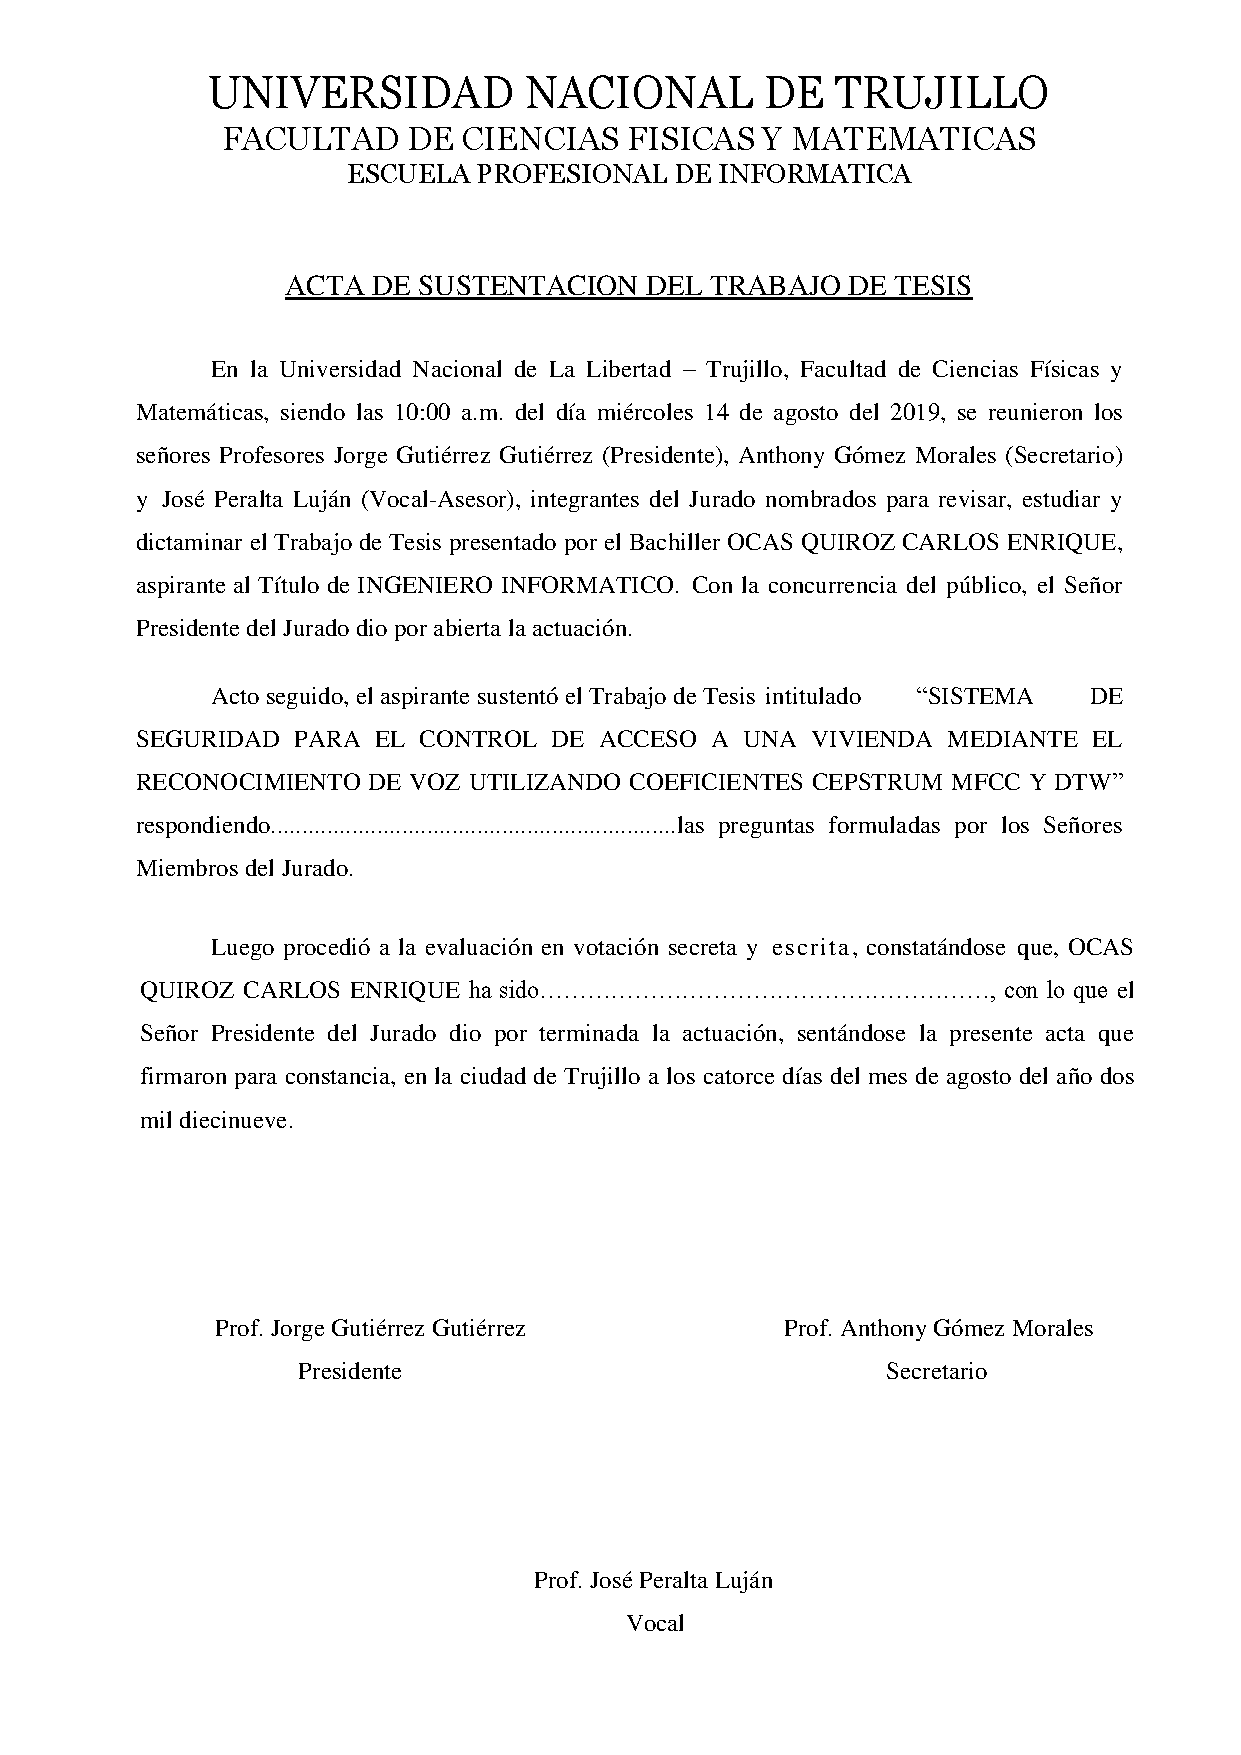
\includepdf[pages=-, offset=75 -75]{Documentos/ACTA_SUSTENTACION1.pdf}

%\setboolean{@twoside}{false}
%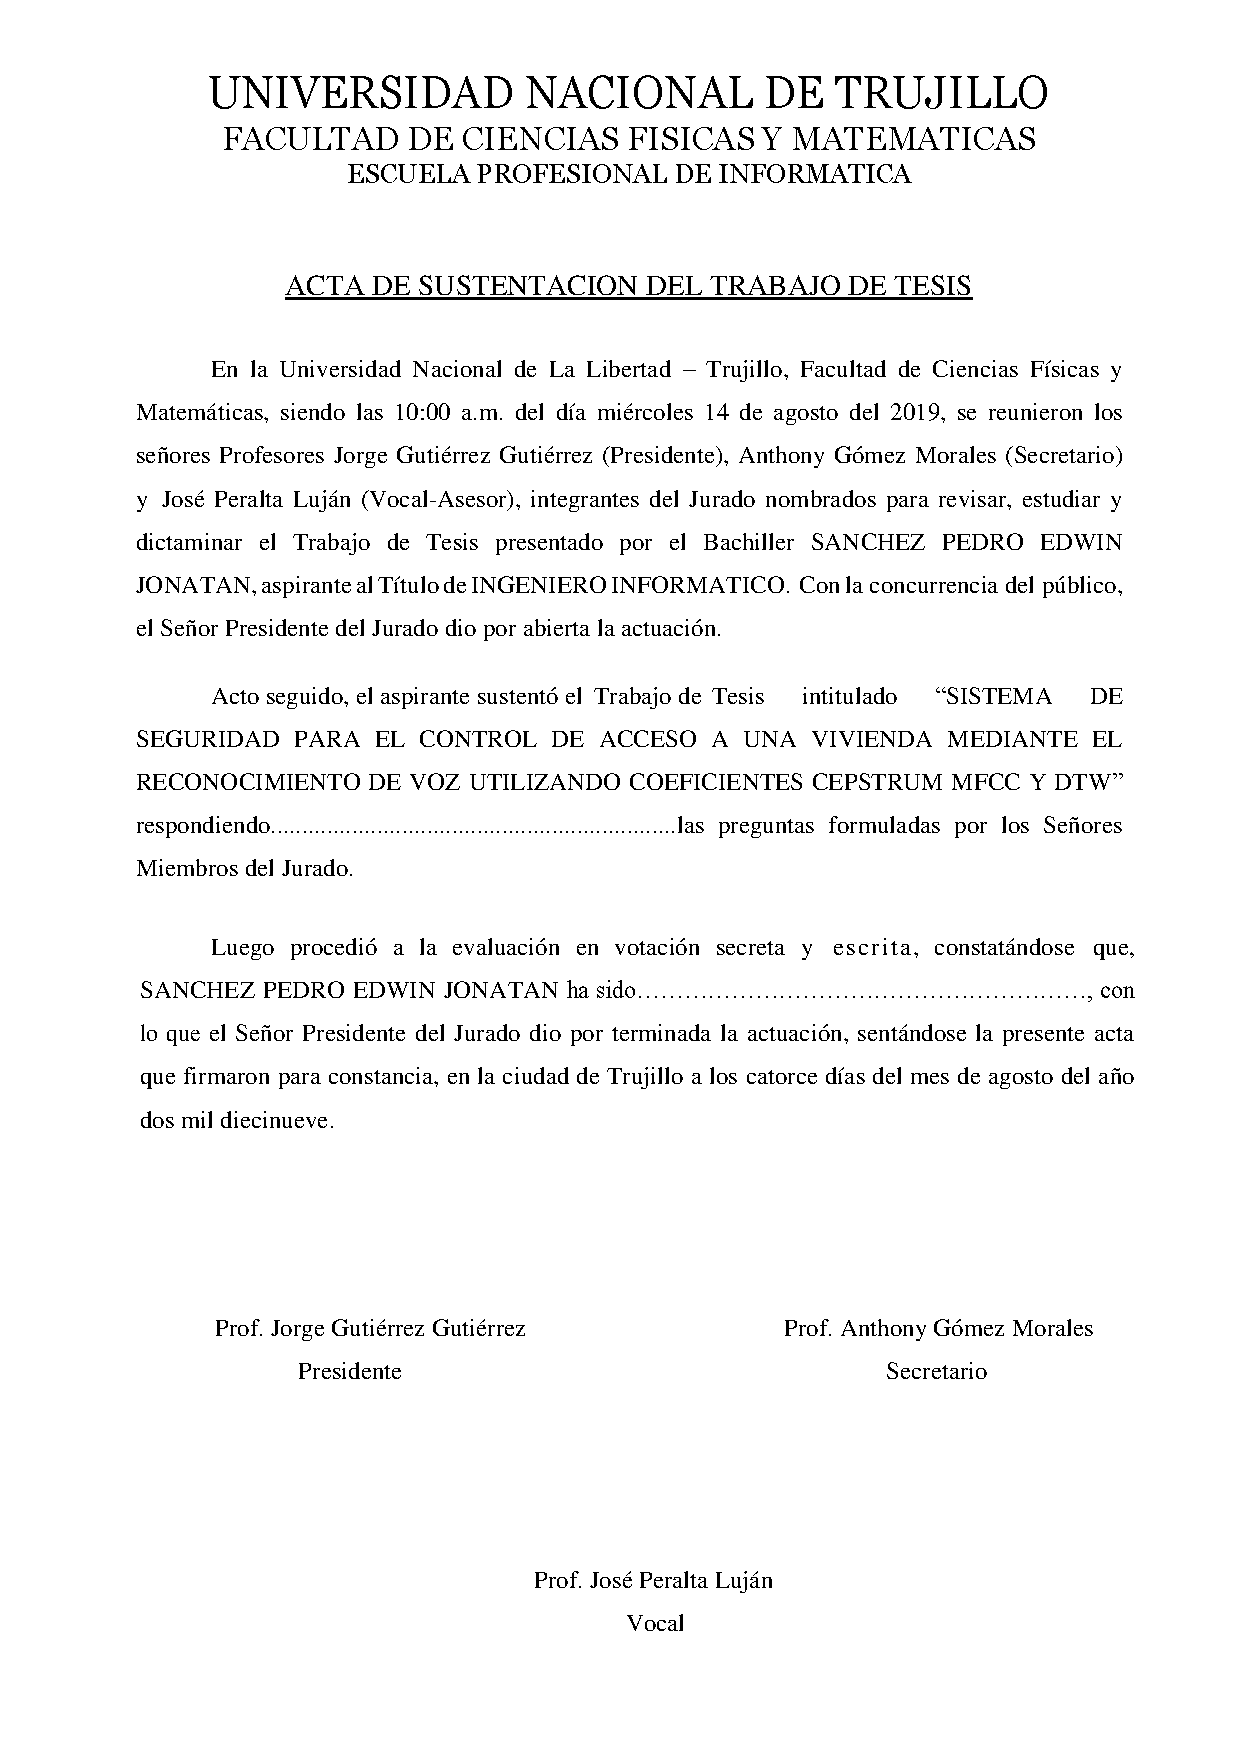
\includepdf[pages=-, offset=75 -75]{Documentos/ACTA_SUSTENTACION2.pdf}
%%%%%%%%%%%%%%%%%%%%%%%%%%%%%%%%%%%%%%%%%%%%%%%%%%%%%%%%%%%%%%%%%%%


%%%%%%%%%%%%%%%%%%%%%%%%%%%% RESUMEN%%%%%%%%%%%%%%%%%%%%%%
\newpage
\begin{center}
 \addcontentsline{toc}{chapter}{Resumen}
 {\bf\LARGE Resumen}
\end{center} 
\begin{quotation}
El presente trabajo de investigación busca desarrollar un sistema de seguridad para el control de acceso a una vivienda mediante el reconocimiento de voz del locutor dependiente del texto, donde el principal objetivo es identificar a cada miembro del hogar, quienes tendrán el acceso.
\vskip 0.1cm
El sistema está conformado por 2 fases, la primera es la de extracción de características de la señal, para esto se usó una adaptación de los MFCC y la segunda es el reconocimiento automático del locutor que esta basada en la técnica DTW, además de una lógica para la toma de decisión en la identificación o no, o falsa identificación de un usuario. En relación a la configuración de los experimentos, para comprobar que el sistema sea confiable se realizaron 2 tipos de pruebas, una entre los usuarios del sistema tratando de acceder uno con el usuario del otro y otra donde personas ajenas a las almacenadas en la base de datos (intrusos) trataron de acceder.
\vskip 0.1cm
Como resultado final, se obtuvo un sistema de seguridad con buenos resultados en el reconocimiento de voz de los miembros del hogar. De esta manera, se pretende contribuir en la industria de sistemas biométricos, en el campo de los sistemas por reconocimiento de voz, así como también poder formar parte de los sistemas domóticos.
\vskip 0.1cm
\hspace*{-0.6cm}{\bf Palabras claves:} Sistema de seguridad, control de acceso, reconocimiento de voz, reconocimiento del locutor, coeficientes cepstrales, alineamiento temporal dinámico.
\end{quotation}
%%%%%%%%%%%%%%%%%%%%%%%%%%%%%%%%%%%%%%%%%%%%%%%%%%%%%%%%%%%%%%%%%%%%%%%%%%%%%%%%%%%%


%%%%%%%%%%%%%%%%%%%%%%%%%%%%ABSTRACT%%%%%%%%%%%%%%%%%%%%%%
\newpage
\begin{center}
 \addcontentsline{toc}{chapter}{Abstract}
 {\bf\LARGE Abstract}
\end{center} 
\begin{quotation}
The present research work seeks to develop a security system for the control of access to a dwelling by voice recognition of the speaker dependent on the text, where the main objective is to identify each member of the household, who will have access.
\vskip 0.1cm
The system consists of 2 phases, the first is the extraction of signal characteristics, for this an adaptation of the MFCC was used and the second is the automatic recognition of the speaker that is based on the DTW technique, in addition to a logic for decision making on the identification or not, or false identification of a user. In relation to the configuration of the experiments, to verify that the system is reliable, 2 types of tests were carried out, one among the users of the system trying to access one with the user of the other and the other where people outside those stored in the database (intruders) tried to access.
\vskip 0.1cm
As a final result, a security system was obtained with good results in the voice recognition of household members. In this way, it is intended to contribute in the biometric systems industry, in the field of voice recognition systems, as well as being able to be part of home automation systems.
\vskip 0.1cm
\hspace*{-0.6cm}{\bf Keywords:} 
Security system, access control, voice recognition, speaker recognition, cepstral coefficients, dynamic time warping.
\end{quotation}
%%%%%%%%%%%%%%%%%%%%%%%%%%%%%%%%%%%%%%%%%%%%%%%%%%%%%%%%%%%%%%%%%%%%%%%%%%%%%%


%%%%%%%%%%%%%%%%%%%%%%%%%%% LISTA DE SIMBOLOS %%%%%%%%%%%%%%%%%%%%%%
\newpage
\addcontentsline{toc}{chapter}{Lista de símbolos}
 {\bf\LARGE Lista de símbolos}
 \vskip 1.5cm
Constantes: 
\begin{enumerate}
\item[(1)]$f_{s}$ \hspace*{0.9cm} Frecuencia de muestreo.
\item[(2)]$f_{max}$ \hspace*{0.45cm} Frecuencia máxima.
\item[(3)]$f_{min}$ \hspace*{0.5cm} Frecuencia mínima.
\item[(4)]$f_{N}$ \hspace*{0.8cm} Frecuencia de Nyquist.
\item[(5)]$T_{s}$ \hspace*{0.9cm} Periodo de muestreo.
\item[(6)]$\mu$ \hspace*{1.05cm} Tamaño de paso de adaptación del filtro adaptivo.
\item[(7)]$M$ \hspace*{0.85cm} Número de orden del filtro adaptivo.
\item[(8)]$\beta$ \hspace*{1.0cm} Constante de adaptación del filtro adaptivo.
\item[(9)]$c$ \hspace*{1.1cm} Constante de normalización del filtro adaptivo.
\item[(10)]$\alpha$ \hspace*{1.0cm} Valor del filtro preénfasis.
\item[(11)]$V$ \hspace*{1.0cm} Longitud de ventana en la segmentación.
\item[(12)]$S$ \hspace*{1.0cm} Valor de desplazamiento o solapamiento en la segmentación.
\item[(13)]$T$ \hspace*{0.9cm} Longitud de trama para la detección de inicio y fin de una palabra.
\item[(14)]$BC$ \hspace*{0.6cm} Número de bandas críticas del MFCC.
\item[(15)]$k_{l}$ \hspace*{0.9cm} Índice correspondiente a la frecuencia inferior.
\item[(16)]$k_{h}$ \hspace*{0.8cm} Índice correspondiente a la frecuencia superior.
\item[(17)]$P$ \hspace*{0.9cm} Slope constraint del DTW.
\item[(18)]$r$ \hspace*{1.0cm} Tamaño de ventana de ajuste del DTW.
\vskip 3cm
\end{enumerate} 
\vskip 0.3cm
Variables:
\begin{enumerate}
\item[(1)] $d(n) $ \hspace*{0.8cm} Señal de voz contaminada.
\item[(2)] $s(n)$ \hspace*{0.8cm} Señal de voz.
\item[(3)] $v_{0}(n)$ \hspace*{0.6cm} Señal de ruido en el micrófono primario.
\item[(4)] $v_{1}(n)$ \hspace*{0.6cm} Señal de ruido en el micrófono secundario.
\item[(5)] $w_{k}(n)$ \hspace*{0.5cm} Vector de pesos del filtro adaptivo.
\item[(6)] $e(n)$ \hspace*{0.8cm} Señal de error o respuesta deseada.
\item[(7)] $E_{n}$ \hspace*{1.0cm} Energía promedio por segmento.
\item[(8)] $E_{avg}$ \hspace*{0.75cm} Energía promedio de toda la señal.
\item[(9)] $M_{n}$ \hspace*{0.9cm} Magnitud promedio.
\item[(10)] $Z_{n}$ \hspace*{1.0cm} Cruce por ceros.
\item[(11)] $M_{sn}$ \hspace*{0.8cm} Magnitud del ruido.
\item[(12)] $Z_{sn}$ \hspace*{0.85cm} Cruce por ceros del ruido.
\item[(13)] $\mu_{Ms}$ \hspace*{0.75cm} Media de la magnitud del ruido.
\item[(14)] $\mu_{Zs}$ \hspace*{0.85cm} Media del cruce por ceros del ruido.
\item[(15)] $\sigma_{Ms}$ \hspace*{0.8cm} Desviación estándar de la magnitud del ruido.
\item[(16)] $\sigma_{Zs}$ \hspace*{0.9cm} Desviación estándar del cruce por ceros del ruido.
\item[(17)] $IZCT$ \hspace*{0.4cm} Umbral de cruce por ceros.
\item[(18)] $ITL$ \hspace*{0.7cm} Umbral de energía bajo.
\item[(19)] $ITU$ \hspace*{0.7cm} Umbral de energía alto.
\item[(20)] $IMX$ \hspace*{0.55cm} Energía máxima de la voz.
\item[(21)] $IMN$ \hspace*{0.7cm} Energía media del ruido de fondo.
\item[(22)] $x_{p}(n)$ \hspace*{0.8cm} Señal de voz con preénfasis.
\item[(23)] $x_{l}(n)$ \hspace*{0.85cm} Señal de voz segmentada.
\item[(24)] $x_{w}(n)$ \hspace*{0.75cm} Señal de voz ponderada.
\item[(25)] $w(n)$ \hspace*{0.9cm} Pesos de la ventana de Hamming.
\item[(26)] $N_{fft}$ \hspace*{1.0cm} Número de puntos de la transformada de Fourier.
\item[(27)] $X(k)$ \hspace*{0.9cm} Espectro en frecuencia de la transformada rápida de Fourier.
\item[(28)] $P(k)$ \hspace*{0.95cm} Espectro en potencia de la transformada rápida de Fourier.
\item[(29)] $\Delta f$ \hspace*{1.2cm} Resolución en frecuencia.
\item[(30)] $SF$ \hspace*{1.2cm} Separación en frecuencia.
\item[(31)] $N_{p}$ \hspace*{1.3cm} Número de puntos del espectro de potencia.
\item[(32)] $\Delta k$ \hspace*{1.2cm} Resolución por muestra del espectro.
\item[(33)] $P_{sc}$ \hspace*{1.2cm} Compresión del espectro en potencia.
\item[(34)] $C_{m}$ \hspace*{1.2cm} Transformada coseno discreta.
\item[(35)] $V_{mfcc}$ \hspace*{0.8cm} Coeficientes MFCC.
\item[(36)] $\Delta C_{k}$ \hspace*{0.8cm} Coeficientes MFCC delta.
\item[(37)] $\Delta \Delta C_{k}$ \hspace*{0.45cm} Coeficientes MFCC doble delta.
\item[(38)] $D_{T}$ \hspace*{1.05cm} Distancia total entre dos vectores.
\item[(39)] $D_{A}$ \hspace*{1.05cm} Distancia acumulada.
\item[(40)] $d$ \hspace*{1.35cm} Medida de distorsión.
\item[(41)] $z_{n}$ \hspace*{1.2cm} Patrón de referencia por la función de alineamiento.
\item[(42)] $U$ \hspace*{1.3cm} Umbral de decisión.
\item[(43)] $P(D)$ \hspace*{0.65cm} Distribución de probabilidad.
\item[(44)] $\mu^{intra}$ \hspace*{0.7cm} Media de las distancias intralocutor.
\item[(45)] $\mu^{inter}$ \hspace*{0.7cm} Media de las distancias interlocutor.
\item[(46)] $\sigma^{intra}$ \hspace*{0.7cm} Desviación estándar de las distancias intralocutor.
\item[(47)] $\sigma^{inter}$ \hspace*{0.7cm} Desviación estándar de las distancias interlocutor.
\end{enumerate}

                % Datos de la tesis
\listoffigures                % Índice de figuras
\addcontentsline{toc}{chapter}{Índice de figuras}
\listoftables                 % Índice de tablas
\addcontentsline{toc}{chapter}{Índice de tablas}
\tableofcontents              % Índice de materias
\chapter{Introducción}
\pagenumbering{arabic}
\setcounter{page}{1}
Hoy en día muchas personas tienen la necesidad de conocer quién y cuando alguien ha tenido acceso, ya sea a una zona de sus viviendas, a cierta información, a un servicio, etc. Por ejemplo, hay centros de trabajo en los que los trabajadores tienen turnos de noche y para poder acceder a su puesto de trabajo necesitan de una llave, ya sea porque a esas horas no hay portero, recepcionista, o simplemente porque la empresa no cuenta con ninguna persona que se encargue de abrirla, debido a esto los empleados deben turnarse para realizar esta tarea, interrumpiendo con esto su jornada laboral y perjudicando su productividad. 
\vskip 0.5cm
Ocurre también que en muchas empresas es conveniente que no todos los empleados tengan acceso a ciertas zonas, por ejemplo, cuando en algunas áreas se trabaja con materiales peligrosos, documentación importante, donde se guarda dinero o material de mucho valor, debido a esto es necesario delimitar estas zonas creando permisos distintos en función de a qué áreas se pueden o no acceder.
\vskip 0.5cm
Debido a estos problemas que ocurren en el día a día, han dado origen a lo que hoy se conoce como \textit{Sistemas de Seguridad para el Control de Acceso}, que es la actividad principal en la seguridad física e informática. El control de acceso es posiblemente la medida de seguridad más importante que se puede establecer, dado que un control bien aplicado nos permite saber quién, cuándo y a que parte se accedió.
\vskip 0.5cm
Es por ello que los controles de acceso facilitan el trabajo a la empresa o lugar donde sea utilizado, estos controles tanto físicos como lógicos se encuentran entre los esquemas de protección imperativos en seguridad. Los controles de acceso físico aseguran que solo el personal autorizado tenga disposición a edificios, salas, documentos, etc. Por otro lado, los controles de acceso lógico protegen las computadoras, las instalaciones de red y los sistemas de información contra amenazas de acceso no autorizado. Estos dos tipos de accesos se basan esencialmente en la autentificación del usuario mediante la cual la identidad de un individuo se verifica a través de uno de los tres medios siguientes: por algo \textit{que conoce}, \textit{que tiene} o \textit{que es} (o por combinaciones de estos).
\vskip 0.5cm
Los sistemas de seguridad han ido evolucionando conforme al avance tecnológico, los primeros sistemas de identificación fueron los \textit{Sistemas de Identificación por Teclado}, donde el usuario utiliza un código o PIN (Número de Identificación Personal) para identificarse. Es económico y práctico porque no requiere identificadores físicos y hace innecesarios las llaves. Si bien este sistema es muy cómodo, presenta un problema que es, que los usuarios pueden compartir la clave fácilmente, lo que compromete la seguridad.
\vskip 0.5cm
Ante este problema aparecieron los \textit{Sistemas de Identificación por Proximidad y Radiofrecuencia}, estos dos métodos cuentan con algo en común que es, que el usuario tiene un artículo identificador. En los \textit{Sistemas de Proximidad}, los usuarios usan tarjetas o llaveros electrónicos para identificarse, estos no necesitan de mantenimiento, aunque sí el sistema, pero su costo es bajo. Por otro lado, los \textit{Sistemas de Radiofrecuencia} son muy comunes en los garajes, a los que se accede con un pequeño mando a distancia, es un sistema cómodo, aunque el tipo de identificador es más costoso que el usado por proximidad. La seguridad que ofrecen estos sistemas es mayor en comparación a un \textit{Sistema de Identificación por Teclado}, ya que un usuario, solo puede utilizar una tarjeta o un llavero a la vez, el problema es que, si perdemos la tarjeta o llavero electrónico, el sistema quedaría inservible y tendría que reconstruirse, ocasionando costos mayores.
\vskip 0.5cm
Debido a este nuevo problema aparecen los \textit{Sistemas de Identificación Biométrica}, la biometría está cada vez más presente en la vida cotidiana de las personas y, sobre todo, en los negocios. El control de acceso biométrico es un sistema de identificación basado en las cualidades fisiológicas del usuario, pero también puede basarse en el comportamiento del mismo, se trata de un sistema personal e intransferible. En \cite{hugo} se dice que, la biometría es más cómoda y segura que los sistemas tradicionales como las contraseñas, llaves o tarjetas.
\vskip 0.5cm
En \cite{cosentino} se dice que, dentro de la biometría como sistema de acceso podemos diferenciar varios tipos de reconocimiento: identificación por geometría de la mano, huella digital, iris y retina y por voz.
\vskip 0.5cm
\textit{El Reconocimiento por Geometría de Mano}, identifica los parámetros dimensionales de la mano, que son únicos. Funciona muy bien, sobre todo en lugares donde no se utilizan guantes y es bastante robusta frente al vandalismo. Los motivos por el cual esta tecnología no se popularizó masivamente son estrictamente comerciales, y es que sólo había un fabricante en el mercado, lo que hizo que los fabricantes de sistemas de control de acceso no ayudaran a difundirla.
\vskip 0.5cm
\textit{El Reconocimiento por Huella Digital}, sin dudas la más popular de todas las biometrías. Es utilizado por los organismos de seguridad y gobiernos para la identificación de personas y/o sospechosos de delitos, y también en los controles de acceso. No son resistentes al vandalismo y uno de los grandes inconvenientes es que la reparación del daño en el elemento sensor es bastante costoso, por lo que se recomienda utilizarlos en lugares no expuestos a estos inconvenientes. Algo similar ocurre con las inclemencias del tiempo, por lo que se deberán extremar los cuidados, si es necesario colocarlos en el exterior y sobre todo expuestos a la intemperie.
\vskip 0.5cm
\textit{El Reconocimiento Facial}, es una tecnología que año a año mejora en sus resultados y si bien actualmente existen fabricantes que ofrecen soluciones de este tipo, todavía no se consiguen equipos comerciales de bajo costo con prestaciones aceptables de identificación y velocidad. Básicamente consiste en identificar y calcular las distancias entre los diferentes accidentes faciales, reduciendo la imagen a un conjunto de coordenadas de puntos significativos.
\vskip 0.5cm
\textit{El Reconocimiento de Iris y Retina}, los equipos de este tipo de reconocimiento funcionan muy bien, tienen un costo relativamente accesible y no tienen contacto físico con el usuario, por lo que pueden ser ubicados detrás de un vidrio de manera de hacerlos resistentes al vandalismo. El inconveniente radica en que no son muy populares, por tratarse de equipos en los que la persona debe mirar adentro y si bien su ojo no tiene contacto con ningún elemento, de todas formas, suelen generar el rechazo de los usuarios.
\vskip 0.5cm
Y por último el \textit{Reconocimiento de Voz}, está tecnología se encuentra en una etapa similar al reconocimiento facial y probablemente algún día sean una alternativa válida.
\vskip 0.5cm
Como podemos observar, las tecnologías biométricas pueden ser una alternativa o un complemento de las técnicas de identificación y autenticación ya existentes. Debido a esto y a la poca producción de sistemas reconocedores de voz, está investigación se basará en este tipo de sistema.
\vskip 0.5cm
Con esto, finalmente podemos decir que la tecnología puede ser una herramienta sumamente útil y poderosa para reducir el riesgo a ser víctimas de intrusos en nuestras viviendas. Es por ello que nos proponemos a diseñar un sistema tecnológico que ayudará a solucionar este problema.

\section{Justificación de la investigación}
Debido a la inseguridad actual que se presenta en la ciudad de Trujillo se realizará un sistema de seguridad para una vivienda por medio de la voz, con la finalidad de proponer a los habitantes de la ciudad un sistema capaz de resguardar su vivienda.
\vskip 0.5cm
Por otro lado, cada vez hay personas menos preparadas en la manipulación de sistemas tecnológicos, debido a la poca familiaridad que tienen con estos, por ello esta investigación propone a los habitantes de la ciudad de Trujillo un sistema simple y fácil de usar.
\vskip 0.5cm
Si bien existen muchos tipos de sistemas de seguridad, donde los biométricos destacan, estos suelen tener un costo elevado para su implementación, debido a que los componentes que se utilizan para la captura y el procesamiento de los datos son caros, siendo así difícil la venta y compra de estos, es por ello que este proyecto servirá como una alternativa ante este problema, permitiendo a la sociedad la adquisición de estos sistemas a un precio cómodo.
\vskip 0.5cm
Además, actualmente no existe ninguna API (Interfaz de Programación de Aplicaciones) de reconocimiento de voz que este de manera gratuita para los desarrolladores de programas informáticos que deseen usar el reconocimiento de voz en sus aplicaciones. Si bien Google ofrece gratuitamente su API de reconocimiento de voz a los desarrolladores de aplicaciones para dispositivos Android, ocurre que para el uso de está API es necesario la conexión a internet, lo que hace que su uso tenga esta limitante, es por ello que nuestro proyecto será una alternativa para aquellos desarrolladores que no cuentan con dinero y acceso a internet, puedan usar esta tecnología en sus programas.

\section{Formulación del problema}
En este trabajo, se propone el desarrollo de un sistema de seguridad para el control de acceso a una vivienda por reconocimiento de voz haciendo uso de los métodos de cuantificación de la señal de voz con ayuda de los MFCC (Coeficientes Cepstrales en la Frecuencia de Mel) y el DTW (Alineamiento Temporal Dinámico) para responder a la siguiente pregunta:
 \begin{center} 
     ?`Cómo controlar el acceso a una vivienda por reconocimiento de voz del locutor dependiente del texto?
 \end{center}

\section{Hipótesis}
El acceso a una vivienda puede ser controlado por reconocimiento de voz del locutor dependiente del texto utilizando MFCC Y DTW.

\section{Objetivos}
\subsection{Generales}
Desarrollar un sistema de seguridad para el control de acceso a una vivienda que funcione en base al reconocimiento de voz.
\subsection{Específicos}
\begin{enumerate}
\item[a)]Recopilar herramientas, técnicas y métodos acústicos matemáticos y físicos de la voz para identificar y autenticar a los dueños de la vivienda.
\item[b)]Analizar la transmisión, aplicación y manipulación de las señales de voz para poderlas utilizar en el desarrollo del sistema de seguridad de control de acceso.
\item[c)]Desarrollar un software que funcione como interfaz con el usuario y que además realice las comparaciones y cálculos necesarios para el reconocimiento del locutor.
\item[d)]Construir un prototipo hardware para el acceso a una vivienda.
\item[e)]Implementar un canal de comunicación inalámbrica entre el hardware y el software.
\end{enumerate}

\section{Estructura de la tesis}
El presente trabajo está dividido en cinco capítulos. El primer capítulo presenta los aspectos generales de la investigación realizada tal como justificación, formulación del problema, la hipótesis, los objetivos y la estructura de la tesis.
\vskip 0.5cm
En el segundo capítulo se presenta el marco referencial teórico y soporte del tema, contemplando los conceptos básicos que se debe de tener en cuenta para el desarrollo de un sistema de seguridad para el control de acceso por reconocimiento de voz, así como algunas consideraciones con respecto al habla. Además, se dará a conocer los métodos y las etapas por las cuales debe pasar un reconocedor de voz para poder procesar y manejar las señales de voz por medio de un software. Finalmente el método empleado en la investigación.
\vskip 0.5cm
El tercer capítulo muestra los procesos para la construcción de nuestro sistema de seguridad para el control de acceso, dividido en tres etapas: la primera la construcción del algoritmo de reconocimiento de voz y su integración en una aplicación Android, la segunda la construcción del prototipo hardware y la tercera el canal de comunicación entre los dos módulos.
\vskip 0.5cm
El cuarto capítulo se muestran los resultados y discusión obtenida en la investigación. El quinto capítulo contiene las consideraciones finales obtenidas en esta tesis. Primero se presentan las conclusiones, seguida de las recomendaciones para futuras investigaciones relacionadas al tema en cuestión. 
\vskip 0.5cm
Por último, las referencias bibliográficas que se usaron para la investigación en esta tesis y en apéndice se presenta el instrumento que se usará para constratar la hipótesis. Finalmente la declaración jurada y la autorización de la tesis.                % Introducción
\chapter{Materiales y métodos}
\section{Marco teórico}
\subsection{Sistema de reconocimiento de voz}

\subsubsection{Historia del reconocedor de voz}
En 1870’s, Alexander Graham Bell, quería construir un dispositivo que hiciera el habla visible a las personas con problemas auditivos, el cual tuvo como resultado el teléfono.
\vskip 0.5cm
En 1880’s, Tihamir Nemes, solicita permiso para una patente de desarrollo de un sistema de transcripción automática que identificara secuencias de sonidos y los imprimiera (texto). Pero fue rechazado como proyecto no realista.
\vskip 0.5cm
En 1910’s, AT\&T Bell Laboratories, construye la primera máquina capaz de reconocer voz basada en plantillas de los 10 dígitos en inglés. Requería un extenso reajuste a la voz de una persona, pero una vez logrado tenía un 99\% de certeza. Por lo tanto, surge la esperanza de que el reconocimiento de voz es simple y directo.
\vskip 0.5cm
En 1940’s y 1950’s, la mayoría de los investigadores reconocen que era un proceso mucho más intrincado y sutil de lo que habían anticipado. Por lo tanto, empiezan a reducir los alcances y se enfocan a sistemas más específicos:

\begin{enumerate}
\item[•]Dependientes del locutor.
\item[•]Flujo discreto del habla (con espacios o pausas entre palabras).
\item[•]Vocabulario pequeño (menor o igual a 50 palabras).
\end{enumerate}

\par
Estos sistemas empiezan a incorporar técnicas de normalización del tiempo (minimizar diferencia en velocidad del habla). Además, ya no buscaban una exactitud perfecta en el reconocimiento, \citep{manfred}. Después IBM y CMV trabajan en reconocimiento de voz continuo, pero no se ven resultados hasta los 1970’s.
\vskip 0.5cm
En 1970’s, un ambicioso proyecto para construir un sistema informático que entienda y procese el habla fue iniciado por DARPA \citep{frederick}, la meta era integrar conocimiento acerca del habla, lingüística e inteligencia artificial para desarrollar un \textit{Sistema Informático del Lenguaje Hablado}. Se desarrolló un sistema informático llamado \textit{Harpy} que integraba todas las fuentes de conocimiento en redes de estado finito, que eran entrenadas estadísticamente. En estos años crecen notoriamente métodos que hacen uso de la probabilidad y se entiende por \textit{Reconocimiento Automático del Habla} como buscar la palabra más probable en una señal de audio, dada alguna información de su distribución de probabilidad.
\vskip 0.5cm
En 1980’s, modernos reconocedores son lanzados al mercado, los algoritmos desarrollados en este tiempo son usados todavía en estos días como: Modelos n-grams, Mixturas Gaussianas, Modelos Ocultos de Markov, Decodificador Viterbi, etc. En 1984 es construido el primer sistema de dictado en tiempo real, por IBM.
\vskip 0.5cm
En 1990’s, con el aumento del poder de cómputo y capacidad de memoria de las computadoras existen avances en algoritmos de adaptación y entrenamiento discriminativo, a la vez se desarrollan sistemas informáticos que reconocían palabras independientemente quien fuera el hablante, algunas de estas aplicaciones fueron implantadas en empresas telefónicas. En 1995, Dragon IBM lanza su producto que reconocía palabras aisladas dependiente del hablante, era un sistema que permitía un dictado de un gran número de palabras. En 1997, Dragon IBM lanza su sistema para dictado continuo. En 2000’s, teléfonos celulares ya ofrecían servicios de marcado activado por voz.
\vskip 0.5cm
En 2010’s, salió a la luz el asistente de voz Siri, realizando funciones de asistente personal a veces con su propia personalidad para iOS, macOS, tvOS y watchOS. Esta aplicación utiliza procesamiento del lenguaje natural para responder preguntas, hacer recomendaciones y realizar acciones mediante la delegación de solicitudes hacia un conjunto de servicios web que ha ido aumentando con el tiempo. También han aparecido asistentes de voz como Cortana de Microsoft y Bixby para dispositivos Android, \citep{timetoast2010}.
\vskip 0.5cm
En la actualidad, se espera que con el poder de cómputo actual de las máquinas y las diversas investigaciones en el tema, se logre aumentar el desempeño. Aplicaciones actuales van desde software para celulares, robótica hasta interfaces de voz para personas discapacitadas; desafortunadamente las comparaciones de error entre humanos y máquinas todavía dan un amplio margen de diferencia, por lo que se espera lograr que éste margen disminuya en los próximos años.

\subsubsection{Fundamentos sobre sonidos y la señal de voz}
La lengua es uno de los órganos más presentes a la hora de hablar, aunque no es el único implicado. En la producción de la voz y en su percepción intervienen muchos órganos y partes del cuerpo (labios, garganta, cerebro, oídos, pulmones, boca, nariz, etc.), sin embargo, hay que tener en cuenta que estas no se emplean solamente para hablar, sino que también desempeñan otras funciones adicionales (comer, respirar, etc.).
\vskip 0.5cm
Ahora veremos algunos conceptos empleados en el estudio de las señales de voz, así como en el funcionamiento de los sistemas generadores de voz, de tal forma que se puedan establecer las características que sirvan para realizar un correcto reconocimiento de voz. Existen varias maneras para analizar y describir el habla. Los enfoques más comúnmente usados son:
\begin{enumerate}
\item[•]\textbf{Articulación:} Análisis de cómo el humano produce los sonidos del habla.
\item[•]\textbf{Señal Acústica:} Análisis de la señal de voz como una secuencia de sonidos.
\item[•]\textbf{Percepción Auditiva:} Análisis de cómo el humano procesa el habla.
\end{enumerate}

\par
Los tres enfoques proveen ideas y herramientas para obtener mejores y más eficientes resultados en el reconocimiento.
\vskip 0.5cm

\begin{enumerate}
\item[a)]Articulación
\par
La voz humana se produce por medio del aparato fonatorio, también llamado aparato bucal o articulatorio, el cual está formado por un conjunto de órganos. El aparato fonador consiste en tres grupos de órganos diferenciados, tal como se ve en la Figura \ref{fig:figura2.1}

\begin{figure}[ht]
\begin{center}
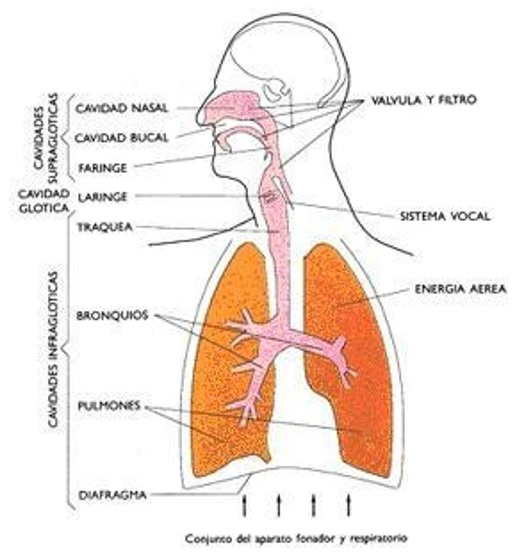
\includegraphics[width=0.4\textwidth]{Imagenes/Cap2/image001}
\end{center}
\begin{center}
\vskip -0.5cm
\caption{\small{Órganos del cuerpo que intervienen en el aparato fonador.}}
\label{fig:figura2.1}
{\small{Fuente: \cite{luis}}}
\end{center}
\end{figure}
\newpage
\begin{enumerate}
\item[•]\textbf{Órganos de respiración o cavidades infraglóticas:} pulmones, bronquios y tráquea.
\item[•]\textbf{Órganos de fonación o cavidades glóticas:} laringe, cuerdas vocales y resonadores nasal, bucal y faríngeo.
\item[•]\textbf{Órganos de articulación o cavidades supraglóticas:} paladar, lengua, dientes, labios y glotis.
\end{enumerate}

\par
El proceso básico de generación de la voz es el mismo ya sea al hablar o al cantar. El cerebro envía señales a través del sistema nervioso a los músculos de la cabeza, cuello y torso de manera que se produzca la inhalación previa a la generación. Al final de la inhalación se efectúan varias acciones, primero se realiza el movimiento de los cartílagos aritenoides en la laringe acercando a las cuerdas vocales entre sí, luego el volumen de los pulmones disminuye para producir una presión de aire positiva en los mismos, después el aire comienza a fluir hacia la laringe generando una excitación y esta adquiere las formas siguientes: fonación, susurro, fricación, compresión y vibración.

\begin{figure}[ht]
\begin{center}
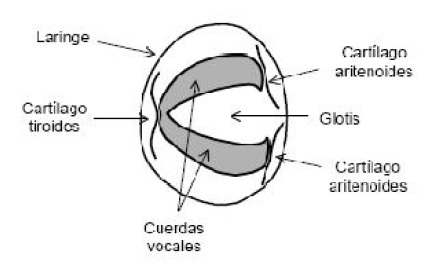
\includegraphics[width=0.3\textwidth]{Imagenes/Cap2/image002}
\end{center}
\begin{center}
\vskip -0.5cm
\caption{\small{Corte esquemático de la laringe en un plano horizontal.}}
\label{fig:figura2.2}
{\small{Fuente: \cite{owens}}}
\end{center}
\end{figure}

\begin{enumerate}
\item[•]Fonación:
\par
Este término se refiere a la oscilación de las cuerdas vocales por los movimientos de los cartílagos aritenoides, cuando el aire es conducido a través de las cuerdas vocales, éstas vibran y sus oscilaciones son dirigidas por la masa y tensión de las cuerdas. La apertura y cierre de las cuerdas secciona el pulso de aire en pulsos cuasiperiódicos llamados pulsos glotales, con una frecuencia fundamental llamada tono. Los sonidos resultantes de la fonación se llaman sonoros, mientras que sonidos con ausencia de fonación se denominan sordos. Así, por ejemplo, las vocales son sonidos sonoros y las consonantes, como la \textit{f}, \textit{s}, \textit{p} y \textit{k}, son sonidos sordos.

\item[•]Susurro:
\par
Los susurros son generados en la laringe. Las cuerdas vocales están juntas por el cartílago aritenoides, pero en lugar de sellar completamente la glotis existe una pequeña apertura triangular entre estos cartílagos, el aire que fluye a través de esta apertura genera turbulencias, que ocasionan ruido de banda ancha, el cual sirve como señal excitadora. Además, los susurros son más débiles que las fonaciones ya que implican un menor volumen de aire, y tienen mayor energía en las altas frecuencias. Sin embargo, se producen sonidos inteligibles si todo un conjunto de sonidos con fonación es reemplazado por susurros de los mismos sonidos. Esto es común cuando se trata de hablar en voz muy baja.

\item[•]Fricación:
\par
La fricación es similar al susurro en cuanto el flujo de aire turbulento genera ruido de banda ancha, pero existe un lugar de articulación adicional en el tracto vocal (dientes, lengua, etc.) Estos sonidos producidos son llamados fricativos, y la fricación puede ocurrir con o sin fonación.
\vskip 0.5cm
Dado que el lugar de articulación es cerca de los labios, sólo una pequeña parte del tracto vocal está entre la fuente de excitación y el aire de salida. Esto significa que la modulación producida por el tracto vocal está limitada en extensión y complejidad. Al igual que el susurro, la fricación es más baja en amplitud que la fonación y tiene una proporción mucho más amplia de las altas frecuencias. Sin embargo, el filtrado muy limitado del tracto vocal, con sus pérdidas menores a bajas frecuencias, permite una mayor radiación de energía, por consiguiente, los sonidos fricativos son más sonoros que los susurros. La fricación puede ocurrir durante interrupciones de fonaciones, esto implica variaciones muy rápidas de amplitud y frecuencia, por lo que juega el papel de modulador.

\item[•]Comprensión:
\par
Cuando el tracto vocal está prácticamente cerrado y una persona sigue exhalando, la presión aumenta y resulta un pequeño transitorio. La combinación de un silencio pequeño seguido por una ráfaga de ruido crea una excitación aperiódica. Si el transitorio es abrupto y limpio, el sonido es una oclusiva o plosiva como en el caso de \textit{p}, si es gradual y turbulento, éste se clasifica como un sonido muy parecido al fricativo, llamado africativo, como en el caso de las letras \textit{ch} e \textit{y}. Las africadas, generalmente, se comportan como un estado intermedio entre oclusivas y fricativas, pero fonéticamente son secuencias de una oclusiva más una fricativa.

\item[•]Vibración:
\par
La vibración es cuasiperiódica y puede ocurrir en muchos lugares del tracto vocal, por ejemplo, la vibrante \textit{r} involucra la vibración de la lengua contra el paladar. Estas vibraciones pueden ocurrir con o sin fonación y su efecto principal es la interrupción.
\end{enumerate}

\par
Las voces del hombre y la mujer difieren debido a varios aspectos, que incluyen el tamaño de la laringe, el tono, el rango de tono, el espacio entre las cuerdas vocales y ocurrencia de problemas del habla. Antes de la pubertad, en promedio el tono y el tamaño de la laringe es el mismo tanto en hombres como en mujeres. La frecuencia fundamental de la voz (la cual está estrechamente relacionada con la percepción del tono) está alrededor de los 250 Hz y la longitud de las cuerdas vocales es de aproximadamente 10.4 mm. 
\vskip 0.5cm
Durante la pubertad, el tamaño de las cuerdas se incrementa en promedio de 5-10 mm. en el caso de los hombres y de 3-5 mm. en el caso de las mujeres. Este aumento reduce el tono promedio a 120 Hz en el hombre y 200 Hz en la mujer. De manera que el tono más alto de la mujer comparado con el hombre es casi una octava, significa que las cuerdas vocales vibran casi el doble de veces por segundo que en los hombres.

\vskip 0.5cm
En resumen, en el habla los formantes se determinan por el proceso de filtrado que se produce en el tracto vocal por la configuración de los articuladores. El sonido particular de la voz de cada persona está determinado por el tamaño y la forma de las cuerdas vocales, de la garganta, de la nariz, de la boca, etc. De tal manera que los sonidos se ven afectados por la forma del tracto vocal.

\vskip 0.5cm
Dada la anterior explicación es necesaria una clasificación acústica, como la que se resume en la Tabla \ref{table:tabla2.1}.

\begin{center}
\begin{table}[h!]
\centering
\caption{\small{Clasificación acústica de los sonidos.}}
\label{table:tabla2.1}
\vskip 0.2cm
\begin{tabular}{|p{4cm}|p{8cm}|p{3cm}|r|}
\hline
{\small Sonidos periódicos compuestos o complejos} & {\small Vibración de la cuerdas vocales(frecuencia fundamental, F0) y resonancia (armónicos)} & {\small Vocales, nasales, laterales}  \\ 
\hline 
{\small Sonidos aperiódicos impulsionales} & {\small Cierre y explosión en el tracto vocal} & {\small Oclusivas}  \\ 
\hline 
{\small Sonidos aperiódicos continuos} & {\small Fricción en el tracto vocal} & {\small Fricativas}  \\ 
\hline 
\end{tabular} 
\begin{center}
\vskip 0.2cm
{\small{Fuente: \cite{joaquim}}}
\end{center}
\end{table}
\end{center}

Los formantes son elementos que sirven para distinguir componentes del habla humana, principalmente, las vocales y sonidos sonantes. El formante con la frecuencia más baja se llama \textit{F1}, el segundo \textit{F2}, el tercero \textit{F3}, etc. Normalmente sólo los dos primeros son necesarios para caracterizar una vocal, aunque la pueden caracterizar más formantes. Generalmente, los formantes posteriores determinan propiedades acústicas como el timbre. Los dos primeros formantes se determinan principalmente por la posición de la lengua. Donde \textit{F1} tiene una frecuencia más alta cuanto más baja esta la lengua, es decir una mayor abertura. Para el \textit{F2} tiene mayor frecuencia cuanto más hacia delante está posicionada la lengua.
\vskip 0.5cm
No todos los sonidos se componen de formantes definidos. Solamente aparecen en sonantes, que incluyen los sonidos pulmonares (vocales y nasales). Los nasales tienen un formante adicional \textit{F3}, en torno a los 1500 Hz. Si la frecuencia fundamental es mayor que la frecuencia de los formantes, entonces el carácter del sonido se pierde y se vuelven difíciles de distinguir, por lo cual son difíciles de reconocer. En la Tabla \ref{table:tabla2.2} se muestran algunos anchos de banda entre los cuales se localizan las vocales:

\begin{center}
\begin{table}[h!]
\centering
\caption{\small{Formantes vocálicos.}}
\label{table:tabla2.2}
\vskip 0.2cm
\begin{tabular}{|c|c|c|}
\hline
{\small Vocal} & {\small Región principal formantica}\\ 
\hline 
{\small /u/} & {\small 200 a 400 Hz}\\ 
\hline 
{\small /o/} & {\small 400 a 600 Hz}\\ 
\hline 
{\small /a/} & {\small 800 a 1200 Hz}\\ 
\hline 
{\small /e/} & {\small 400 a 600 Hz y 2200 a 2600 Hz}\\ 
\hline 
{\small /i/} & {\small 200 a 400 Hz y 3000 a 3500 Hz}\\ 
\hline 
\end{tabular} 
\begin{center}
\vskip 0.2cm
{\small{Fuente: \cite{wikipedia1}}}
\end{center}
\end{table}
\end{center}

\newpage
\item[b)]Señal acústica
\par
Un reconocedor no puede analizar los movimientos en la boca. En su lugar, la fuente de información es la señal de voz misma. El habla es una señal analógica, es decir, un flujo continuo de ondas sonoras y silencios. El conocimiento de la ciencia de la acústica se utiliza para identificar y describir los atributos del habla que son necesarios para un reconocimiento de voz efectivo, \cite{luis}.
\vskip 0.5cm
Algunas características importantes del análisis acústico son:
\begin{enumerate}
\item[•]Frecuencia y amplitud:
\par
Todos los sonidos causan movimientos entre las moléculas del aire. Los sonidos más simples son los sonidos puros, y se pueden representar gráficamente por una onda senoidal. 
\vskip 0.5cm
La frecuencia es el número de vibraciones (ciclos) del tono por segundo y se mide en Hz (hertz), donde los tonos altos tienen mayor frecuencia y los tonos bajos tienen menor frecuencia.
\vskip 0.5cm
El volumen de un sonido refleja la cantidad de aire que es forzada a moverse. Esta describe y representa como amplitud de la onda y se mide en dBC (decibéles).
\vskip 0.5cm

\item[•]Resonancia:
\par
La resonancia se define comúnmente como la habilidad que tiene una fuente vibrante de sonido de causar que otro objeto vibre gracias a ella. La mayoría de los sonidos incluyendo el habla tienen una frecuencia dominante llamada frecuencia fundamental, también conocida como pitch (tono) que se combina con frecuencias secundarias en el habla, la frecuencia fundamental es la velocidad a la que vibran las cuerdas vocales al producir un fonema sonoro. Sumadas a la frecuencia fundamental hay otras frecuencias que contribuyen al timbre del sonido (lo que nos permiten distinguir una trompeta de un violín, las voces de diferentes personas, etc.). Algunas bandas de la frecuencia secundarias juegan un rol importante en la distinción de un fonema de otro. Se les llama formantes y son producidas por la resonancia, tal y como vimos anteriormente.

\item[•]Estructura armónica y ruido:
\par
El habla no es un tono puro es continuación de múltiples frecuencias y se representa como una onda compleja. Las vocales se componen de 2 o más ondas simples, ricos en frecuencias secundarias y contienen estructuras internas de ondas cíclicas y acíclicas.
\vskip 0.5cm
Las ondas acíclicas no tienen patrones repetitivos, son llamados ruido y forman parte de todos los fonemas sonoros, consonantes y semivocales. Las frecuencias y características de estas ondas proveen información importante sobre la identidad de los fonemas.
\vskip 0.5cm
La identidad de las consonantes también se revela por el cambio en las formantes que resultan cuando los articuladores se mueven de un fonema anterior a la consonante y de ella al siguiente fonema llamadas transiciones de formantes. Estas se analizan utilizando técnicas como FFT (Transformada Rápida de Fourier) generando espectrogramas.
\vskip 0.5cm
La complejidad de las formas de onda de los fonemas y las constantes transiciones de un patrón a otro dificultan el análisis de los patrones utilizando las representaciones complejas de las ondas. Los patrones armónicos y de ruido se muestran con más claridad utilizando los espectrogramas de banda ancha. La localización (la distancia entre ellas) y cambio en las formantes ayudan a identificar fonemas y palabras.

\item[•]Coarticulación:
\par
Los fonemas aparentemente tienen parámetros acústicos claramente definidos, pero más bien, los fonemas tienden a ser abstracciones implícitamente definidas por la pronunciación de palabras en un lenguaje. La forma acústica de un fonema depende fuertemente del contexto acústico en el que sucede, a éste efecto se le llama coarticulación. Los investigadores, utilizan este concepto para distinguir entre la característica conceptual de un sonido del habla y una instancia o pronunciación específica de ese fonema, \cite{franco}.
\end{enumerate}

\newpage
\item[c)]Percepción auditiva
\par
La variabilidad del habla producida por coarticulación y otros factores hacen del análisis de la voz extremadamente difícil.
\vskip 0.5cm
La facilidad del humano en superar estas dificultades sugiere que un sistema basado en la percepción auditiva podría ser un buen enfoque desafortunadamente el conocimiento de la percepción humana es incompleto, lo que se sabe es que el sistema auditivo está adaptado a la percepción de la voz.
\vskip 0.5cm
El oído humano detecta frecuencias de 20 a 20000 Hz, pero es más sensible al rango entre 1000 y 6000 Hz, además de los pequeños cambios en la frecuencia en el ancho de banda, crítico para el habla. El patrón de sensibilidad a cambios en el tono no corresponde a la escala lineal de frecuencias de ciclos por segundo de la acústica. Para representar mejor al patrón de percepción acústica, se tiene una escala llamada \textit{Escala de Mel}, la cual es una escala logarítmica que representa los niveles de la señal.
\vskip 0.5cm
El humano no procesa frecuencias individuales independientemente, como lo sugiere el análisis acústico. En su lugar escucha grupos de frecuencias por lo cual es capaz de distinguirlas de ruidos alrededor, \cite{eyra}.
\end{enumerate}

\subsubsection{Modelo digital para la voz (Fuente-Filtro)}
Una forma bastante simplificada pero efectiva para comprender el mecanismo para la producción de la voz es mediante el modelo fuente-filtro, propuesto originalmente por Muller en 1848. En dicho modelo, se supone que la fuente o señal de excitación es linealmente separable de las características del tracto vocal, que se representan por medio de un filtro. Por lo tanto, la señal de voz es la salida de este filtro en respuesta a la fuente de excitación, la cual puede representarse como un generador de un tren de impulsos cuasiperiódicos para los sonidos sonoros, o como un generador de ruido aleatorio (ruido blanco) para los sonidos sordos, \cite{rowden}.
\vskip 0.5cm
Puesto que el filtro debe tener las mismas características que el tracto vocal, no es posible mantener constantes los parámetros del filtro, los cuales tienen que ser modificados para que correspondan a las variaciones que suceden al hablar. Por lo tanto, el filtro tiene parámetros variantes en el tiempo. No obstante, en la práctica, esta tasa de cambio varía lentamente en el tiempo, por lo que los parámetros tienen que ser actualizados en intervalos de 5 a 30 ms.
\vskip 0.5cm
La Figura \ref{fig:figura2.3} muestra un diagrama de bloques del modelo fuente-filtro. El modelo es relevante porque para cada tipo de excitación, un fonema se identifica principalmente por la forma del tracto vocal, por lo que su configuración puede ser estimada al identificar el filtrado realizado por este.

\begin{figure}[ht]
\begin{center}
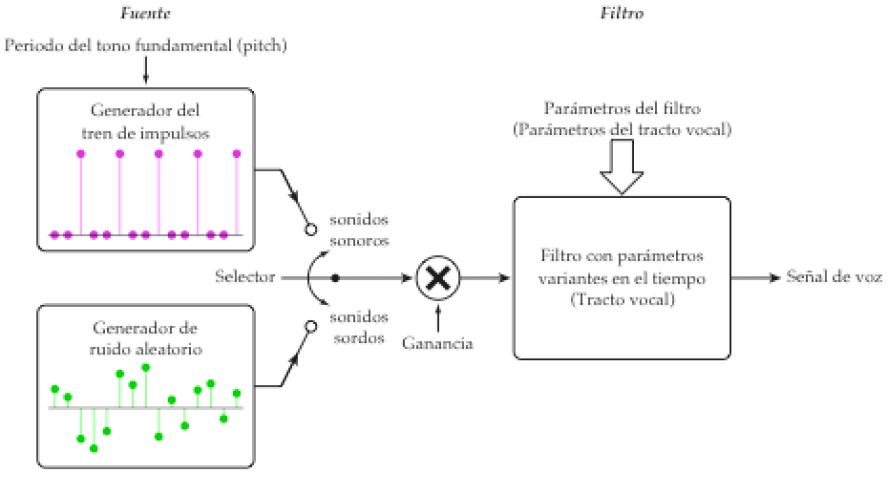
\includegraphics[width=0.5\textwidth]{Imagenes/Cap2/image003}
\end{center}
\begin{center}
\vskip -0.5cm
\caption{\small{Modelo fuente-filtro para la producción de la voz.}}
\label{fig:figura2.3}
{\small{Fuente: \cite{rowden}}}
\end{center}
\end{figure}

\subsubsection{Funcionamiento de un sistema de reconocimiento de voz}
El reconocimiento de voz generalmente es utilizado como una interfaz entre humano y computador para algún software, tal es el caso, por ejemplo, el de los sistemas biométricos. Todo sistema de reconocimiento de voz debe cumplir las 3 tareas siguientes:

\begin{enumerate}
\item[•]\textbf{Preprocesamiento:} Convierte la entrada de voz a una forma que el reconocedor pueda procesar.
\item[•]\textbf{Reconocimiento:} Identifica lo que se dijo (traducción de señal a texto).
\item[•]\textbf{Comunicación:} Envía lo reconocido al sistema (hardware/software) que lo requiere.
\end{enumerate}

En la Figura \ref{fig:figura2.4} se muestran los componentes de un sistema de reconocimiento de voz:

\newpage
\begin{figure}[ht]
\begin{center}
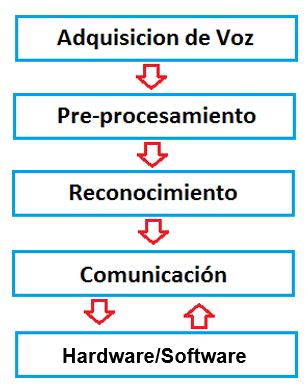
\includegraphics[width=0.25\textwidth]{Imagenes/Cap2/image004}
\end{center}
\begin{center}
\vskip -0.5cm
\caption{\small{Diagrama de bloques del proceso general del reconocimiento de voz.}}
\label{fig:figura2.4}
{\small{Fuente: \cite{rama}}}
\end{center}
\end{figure}

Existe una comunicación bilateral en aplicaciones en las que la interfaz de voz está íntimamente relacionada al resto de la aplicación. Estas pueden guiar al reconocedor especificando las palabras o estructuras que el sistema puede utilizar. Otros sistemas tienen una comunicación unilateral.
\vskip 0.5cm
Los procesos de preprocesamiento, reconocimiento y comunicación deberían ser invisibles al usuario de la interfaz. El usuario lo nota en el desempeño del sistema de manera indirecta como: certeza en el reconocimiento y velocidad. Estas características se utilizan para evaluar una interfaz de reconocimiento de voz.
\vskip 0.5cm
Una vez visto el proceso general de un sistema de reconocimiento de voz, a continuación, veremos los módulos necesarios a detalle para el diseño y construcción de un sistema de reconocimiento de voz del locutor dependiente del texto. 
\vskip 0.5cm
Los diagramas de bloques que se muestran en las Figuras \ref{fig:figura2.5} y \ref{fig:figura2.6} ilustran, de forma general, los procesos que se realizan en el entrenamiento y reconocimiento de palabras aisladas, respectivamente.

\begin{figure}[ht]
\begin{center}
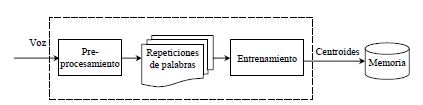
\includegraphics[width=0.55\textwidth]{Imagenes/Cap2/image005}
\end{center}
\begin{center}
\vskip -0.5cm
\caption{\small{Diagrama de bloques para la etapa de entrenamiento.}}
\label{fig:figura2.5}
{\small{Fuente: \cite{navarrete}}}
\end{center}
\end{figure}

\begin{figure}[ht]
\begin{center}
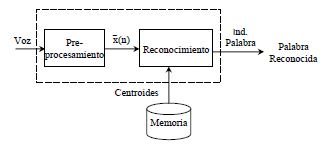
\includegraphics[width=0.5\textwidth]{Imagenes/Cap2/image006}
\end{center}
\begin{center}
\vskip -0.5cm
\caption{\small{Diagrama de bloques para la etapa de reconocimiento.}}
\label{fig:figura2.6}
{\small{Fuente: \cite{navarrete}}}
\end{center}
\end{figure}

Si observamos las Figuras \ref{fig:figura2.5} y \ref{fig:figura2.6}, existe un módulo común en ambas etapas, el preprocesamiento. Por esta razón, el preprocesamiento se manejará como un módulo independiente, para efecto del análisis.
\vskip 0.5cm
En la Figura \ref{fig:figura2.5}, durante la etapa de entrenamiento se capturan diferentes señales de voz, a la que denominaremos repeticiones de palabras. A cada repetición se le aplica preprocesamiento para obtener una palabra delimitada, después se agrupan todas las palabras recortadas y con ellas se obtienen sus centroides correspondientes, para luego ser guardados en memoria (base de datos).
\vskip 0.5cm
Como se observa en la Figura \ref{fig:figura2.6}, en la etapa de reconocimiento se captura la palabra que se desea reconocer. A esta palabra, también se le aplica preprocesamiento, para recortarla. Utilizando los centroides, calculados durante el entrenamiento y almacenados en la memoria, se realizan las comparaciones necesarias, para efectuar el reconocimiento. El éxito del evento dependerá de ciertos parámetros estadísticos obtenidos mediante el análisis de una población de resultados.

\subsection{Procesamiento o análisis de la señal de voz}
La finalidad del procesamiento de la señal de voz es obtener una representación más útil o conveniente de la información contenida en esta. Como se mostró anteriormente, la señal de voz es una composición compleja de sonidos, pero mediante un análisis, se puede mostrar que está formada por la combinación de componentes a diferentes frecuencias, producidas por la excitación periódica o aperiódica de las resonancias en el tracto vocal, principalmente entre 80 y 8000 Hz, \cite{rowden}.
\vskip 0.5cm
Las técnicas de análisis se pueden clasificar en dos categorías: en el dominio del tiempo o en el dominio de la frecuencia. Los procedimientos en el dominio del tiempo, se denominan así, porque éstos tienen que ver directamente con la señal de voz. El atractivo de estas representaciones es la facilidad con la que se pueden implementar, no obstante, estas suministran un medio útil para estimar otras características importantes de la señal. En contraste, los métodos en el dominio de la frecuencia involucran, ya sea de manera explícita o implícita, alguna forma de representación del espectro en frecuencia. 
\vskip 0.5cm
La mayoría de estas se basan en el modelo fuente-filtro, visto anteriormente, para la producción de la voz. Así que esencialmente, el análisis es el proceso en el cual, a partir de una señal de voz, se estiman los parámetros variantes en el tiempo del filtro, de tal manera que su objetivo principal es el estimar la respuesta en frecuencia del filtro que representa al tracto vocal. 
\vskip 0.5cm
A continuación, veremos los conceptos necesarios para la construcción de un reconocedor de voz, por cada una de las etapas que este tiene.

\subsubsection{Preprocesamiento}
En el preprocesamiento se recibe una señal de voz y se digitaliza determinando sus límites, esta señal puede contener ruido externo o no, si la contiene se aplicará un filtro de eliminación de ruido. Luego a la señal se le aplica un filtro de preénfasis, para realzar las frecuencias altas presentes en la voz. Después se divide la señal en tramas y a cada trama se le aplica una ventana para suavizar el espectro. 
\vskip 0.5cm
Es necesario aclarar que, cuando se inicializa el sistema, se determinan ciertos parámetros (umbrales) necesarios para la detección de inicio y fin de la señal de voz. Estos parámetros se calculan recolectando muestras del ruido presente en el ambiente circundante. El módulo encargado de realizar este proceso se denomina ruido ambiental. Finalmente, con las tramas provenientes del ventaneo y con los umbrales originados por el ruido ambiental, se determina el inicio y fin de la señal de voz, tal como se muestra en la Figura \ref{fig:figura2.7}.
\vskip 0.5cm
Como ya se mencionó, el preprocesamiento es un módulo presente en las etapas de entrenamiento y reconocimiento. Sin embargo, existe una diferencia sutil, durante el entrenamiento cada palabra recortada se almacena, y en un archivo independiente se determinan los centroides representativos de esta, mientras que en el reconocimiento se utiliza directamente el archivo con los centroides para hacer las comparaciones. La Figura \ref{fig:figura2.7} muestra el diagrama de bloques para este módulo.

\begin{figure}[ht]
\begin{center}
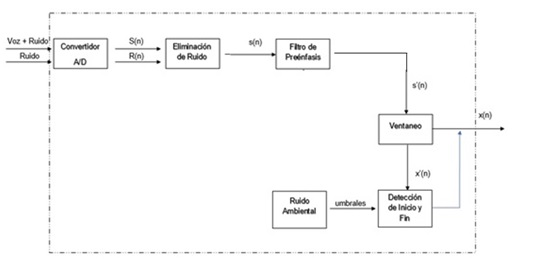
\includegraphics[width=0.83\textwidth]{Imagenes/Cap2/image007}
\end{center}
\begin{center}
\vskip -0.5cm
\caption{\small{Diagrama de bloques para el módulo de preprocesamiento.}}
\label{fig:figura2.7}
{\small{Fuente: Adaptación de \cite{navarrete}}}
\end{center}
\end{figure}

\newpage
El preprocesamiento consta de los siguientes módulos: convertidor A/D, eliminación de ruido, filtro de preénfasis, ventaneo o segmentación, detección de ruido ambiental y detección de inicio y fin de la señal de voz. Estos módulos se describen a continuación:

\begin{enumerate}
\item[a)]Digitalización de la señal de voz
\par
Para poder manipular la señal de voz esta debe de ser transformada a una señal digital, así podrá ser utilizada por el software de programación, este proceso se lleva a cabo en etapas con consideraciones variables que hacen que la adquisición de la señal sea de forma correcta.

\vskip 0.5cm
\begin{figure}[ht]
\begin{center}
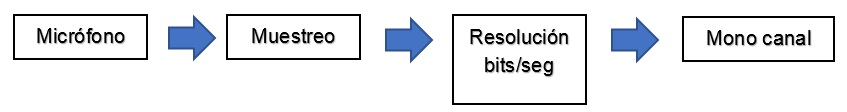
\includegraphics[width=0.6\textwidth]{Imagenes/Cap2/image008}
\end{center}
\begin{center}
\vskip -0.5cm
\caption{\small{Diagrama de la adquisición de voz.}}
\label{fig:figura2.8}
{\small{Fuente: \cite{eyra}}}
\end{center}
\end{figure}

\begin{figure}[ht]
\begin{center}
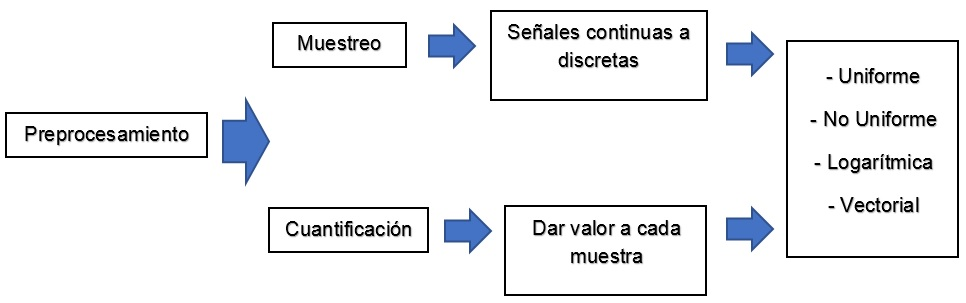
\includegraphics[width=0.6\textwidth]{Imagenes/Cap2/image009}
\end{center}
\begin{center}
\vskip -0.5cm
\caption{\small{Diagrama de la digitalización de la señal de voz.}}
\label{fig:figura2.9}
{\small{Fuente: \cite{eyra}}}
\end{center}
\end{figure}

\newpage
\begin{enumerate}
\item[•]Obtención de información mediante un micrófono
\par
El micrófono es un transductor electroacústico. Su función es la de transformar la presión acústica ejercida sobre su capsula por las ondas sonoras en energía eléctrica.
\vskip 0.5cm
Como se dijo, el audio es un fenómeno analógico. Para grabar una señal de voz se hace la conversión de la señal analógica del micrófono en una señal digital por medio del conversor A/D en la tarjeta de sonido. Cuando un micrófono está operando las ondas de sonido hacen que vibre el elemento magnético del micrófono, causando una corriente eléctrica hacia la tarjeta de sonido, donde el conversor A/D básicamente graba los voltajes eléctricos en intervalos específicos.
\vskip 0.5cm
Hay dos factores importantes durante este proceso. Primero está la taza de muestreo, es decir que tan seguido los valores de voltaje son grabados. Segundo, son los bits por segundo, en otras palabras, que tan exactamente los valores son grabados. Un tercero podría ser el número de canales (mono o estéreo), pero para las aplicaciones de reconocimiento de voz un canal (mono) es suficiente.

\item[•]Ancho de banda y muestreo
\par
Según \cite{claudio}, el ancho de banda para las señales de voz es de aproximadamente unos 16000 Hz, pero la mayor parte de la energía se concentra en las frecuencias menores a 7000 Hz. No obstante, un ancho de banda de 3500 Hz es suficiente para poder entender el mensaje contenido en la señal de voz.
\vskip 0.5cm
El valor para la frecuencia de muestreo se determina mediante el teorema del muestreo de Nyquist, que establece que, si la componente en frecuencia más alta presente en la señal de voz es \textit{$f_{max}$}, entonces para poder reconstruir apropiadamente la señal a partir de las muestras obtenidas, la frecuencia de muestreo \textit{$f_{s}$} debe satisfacer la siguiente condición:
\begin{center}
$f_{s} \geq 2f_{max}$ \hspace{1cm} $f_{N} \doteq f_{max}$ \hspace{1cm} $f_{s} \geq 2f_{N}$
\end{center}
En donde a $f_{N}$ se le conoce como la frecuencia de Nyquist. Por lo tanto, el periodo de muestreo $T_{s}$ es igual al inverso de la frecuencia de muestreo \textit{$f_{s}$}:
\begin{center}
$T_{s} \doteq \frac{1}{f_{s}}$
\end{center}
Si se emplea una frecuencia de muestreo menor que el doble de la frecuencia de Nyquist, entonces sucede un fenómeno conocido como \textit{aliasing}, para el cual una señal senoidal a cierta frecuencia pudiera parecer otra señal de menor frecuencia, como si esta fuera un alias de la original. Si ocurriera un aliasing en la señal de voz, se insertarían algunas componentes en frecuencia no deseadas que la distorsionarían.
\newpage
Puesto que el ancho de banda de una señal de voz se reduce durante la conversión A/D (analógico/digital), para su procesamiento se suelen utilizar básicamente dos frecuencias de muestreo, la primera de \textit{$f_{s}$ = 16000 Hz} para obtener un ancho de banda o una frecuencia de Nyquist de \textit{$f_{N}$ = 8000 Hz}, y la segunda de \textit{$f_{s}$ = 8000 Hz} que corresponde a un ancho de banda o una frecuencia de Nyquist de \textit{$f_{N}$ = 4000 Hz}, \cite{claudio}.
\vskip 0.5cm
En cualquier caso, el muestreo periódico de una señal analógica de voz \textit{x(t)}, proporciona una representación de esa señal mediante una secuencia de muestras \textit{x(n)}, que se pueden obtener mediante la siguiente relación:
\begin{center}
$x(n) \doteq x(t) \textbf{|}_{t \doteq nT_{s}}$ \hspace{1cm} $n \doteq 0,1,2,3,...,N_{x} - 1$
\end{center}
En donde $N_{x}$ es el número total de muestras presentes en la señal de voz. La Figura \ref{fig:figura2.10} ilustra el muestreo de una señal analógica de voz a una frecuencia de muestreo de \textit{$f_{s}$ = 8000 Hz}, así que cada una de las \textit{$N_{x}$ = 21} muestras se toman cada \textit{$T_{s}$ = 0.125 ms}.
\vskip 0.5cm
\begin{figure}[ht]
\begin{center}
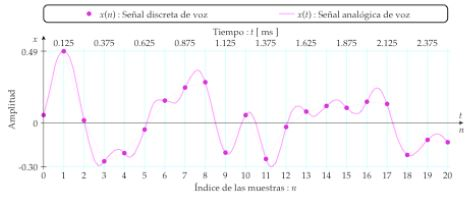
\includegraphics[width=0.7\textwidth]{Imagenes/Cap2/image010}
\end{center}
\begin{center}
\vskip -0.5cm
\caption{\small{Muestreo de una señal de voz.}}
\label{fig:figura2.10}
{\small{Fuente: \cite{claudio}}}
\end{center}
\end{figure}

La señal discreta de voz \textit{x(n)} esta indizada por la variable \textit{n}, que da una normalización de la señal, es decir, que ésta no contiene ninguna información explícita acerca de la frecuencia de muestreo. Aunque las muestras definen una señal discreta, se acostumbra unir éstas para que formen una curva continua para representar la señal de voz.

\item[•]Resolución o cuantificación
\par
El proceso de cuantificación es uno de los pasos que se siguen para lograr la digitalización de una señal analógica. Este proceso convierte una sucesión de muestras de amplitud continua en una sucesión de valores discretos preestablecidos según el código utilizado, \cite{manfred}.
\vskip 0.5cm
Durante el proceso de cuantificación se mide el nivel de tensión de cada una de las muestras, obtenidas en el proceso de muestreo, y se les atribuye un valor finito de amplitud, seleccionado por aproximación dentro de un margen de niveles previamente fijado.
\vskip 0.5cm
En la Figura \ref{fig:figura2.11} se muestra un ejemplo utilizando 2 bits donde se pueden representar 4 valores diferentes y con 4 bits 16 valores.
\vskip 0.5cm
\begin{figure}[ht]
\begin{center}
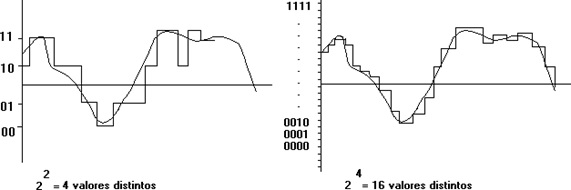
\includegraphics[width=0.7\textwidth]{Imagenes/Cap2/image011}
\end{center}
\begin{center}
\vskip -0.5cm
\caption{\small{Señal cuantificada con 2 y 4 bits respectivamente.}}
\label{fig:figura2.11}
{\small{Fuente: \cite{eyra}}}
\end{center}
\end{figure}

Esto se puede ver como la resolución:
\begin{enumerate}
\item[-]El error o diferencia entre la señal original y la reconstruida se percibe como ruido.
\item[-]Por lo tanto, a mayor resolución menor ruido como consecuencia.
\item[-]La resolución (número de bits por muestra) se describe generalmente en términos de la relación señal a ruido (Signal to Noise Ratio o SNR).
\item[-]A mayor SNR es mayor la fidelidad de la señal digitalizada.
\item[-]SNR es aproximadamente $2^B$ (B=bits/muestra)
\item[-]Es independiente de la frecuencia de muestreo.
\end{enumerate}

Existen diferentes técnicas de cuantificación, a continuación, explicaremos cada una de ellas:
\begin{enumerate}
\item[-]Cuantificación uniforme
\par
En los cuantificadores uniformes o lineales la distancia entre los niveles de reconstrucción es siempre la misma, la mayoría usan un número de niveles que es una potencia de 2. No hacen ninguna suposición acerca de la señal a cuantificar, de allí que no proporcionen los mejores resultados. Su ventaja es que son más fáciles y económicos al implementarlos.
\begin{figure}[ht]
\begin{center}
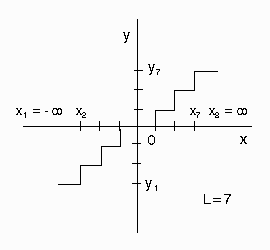
\includegraphics[width=0.3\textwidth]{Imagenes/Cap2/image012}
\end{center}
\begin{center}
\vskip -0.5cm
\caption{\small{Señal cuantificada uniformemente.}}
\label{fig:figura2.12}
{\small{Fuente: \cite{rama}}}
\end{center}
\end{figure}

\item[-]Cuantificación no uniforme
\par
El problema de la cuantificación uniforme es que conforme aumenta la amplitud de la señal, también aumenta el error. Si conocemos la función de la distribución de probabilidad, podemos ajustar los niveles de reconstrucción a la distribución de forma que se minimice el error cuadrático medio. Esto significa que la mayoría de los niveles de reconstrucción se den en la vecindad de las entradas más frecuentes, y consecuentemente se minimice el error.
\newpage
\begin{figure}[ht]
\begin{center}
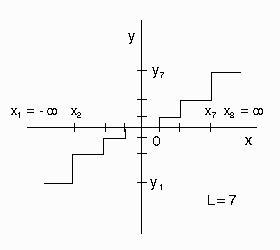
\includegraphics[width=0.3\textwidth]{Imagenes/Cap2/image013}
\end{center}
\begin{center}
\vskip -0.5cm
\caption{\small{Señal cuantificada no uniformemente.}}
\label{fig:figura2.13}
{\small{Fuente: \cite{rama}}}
\end{center}
\end{figure}

\item[-]Cuantificación logarítmica
\par
Las señales de voz pueden tener un rango dinámico mayor a los 60 dBC, por lo que para conseguir una alta calidad de voz se deben usar un elevado número de niveles de reconstrucción. Sin embargo, interesa que la resolución sea mayor en las partes de la señal de menor amplitud que en las de mayor amplitud. Por tanto, en la cuantificación lineal se desperdician niveles de reconstrucción y ancho de banda. Esto se puede mejorar incrementando la distancia entre los niveles de reconstrucción conforme aumenta la amplitud de la señal. Para conseguir esto se hace pasar la señal por un compresor logarítmico antes de la cuantificación. Esta señal comprimida puede ser cuantificada uniformemente. Luego a la salida del sistema la señal pasa por un expansor. A esta técnica se le llama compresión, \cite{harrington}.

\item[-]Cuantificación vectorial
\par
Este método cuantifica los datos en bloques de N muestras, cada bloque se trata como un vector N-dimensional. La cuantificación vectorial ofrece mejores resultados que la cuantificación escalar, sin embargo, es más sensible a los errores de transmisión y lleva consigo una mayor complejidad computacional.
\end{enumerate}
La cuantificación más usada, es de 8 bits, mínimo requerido para una calidad baja, puede mejorarse su SNR con una técnica no lineal de cuantificación, pero se obtienen excelentes resultados aumentando la cuantificación a 16 bits, \cite{kaifu}.
\end{enumerate}

\item[b)]Eliminación de ruido y normalización
\par
El ruido es como una señal no deseada, es un elemento independiente de la señal, pero como consecuencia puede afectar la calidad de la misma. Para cancelar el ruido y mejorar la calidad se han desarrollado diversas técnicas de procesamiento de señal, dentro de los cuales se puede mencionar los filtros adaptativos, que es una técnica de las varias que existen hoy en día y es importante considerar los tipos de ruidos existentes en los canales de comunicación, \cite{henry}.

\begin{enumerate}
\item[-]Ruido aditivo: Se puede considerar todo aquel ruido procedente de distintas fuentes que coexistan en el mismo entorno acústico.
\item[-]Señales interferentes: En el caso de señales de voz, se considera señal interferente a toda aquella que proceda de otros locutores, que no sean objeto de interés.
\item[-]Reverberación: Producida por la propagación multitrayectoria que se dan en los entornos acústicos cerrados o semicerrados. No se trata exactamente de ruido, sino de una forma de distorsión.
\item[-]Eco: Producida generalmente por el acoplamiento entre los micrófonos y los altavoces. Igual que en el caso anterior se trata de una forma de distorsión.
\item[-]Diafonía: Sonido indeseado que se origina en el receptor, y es la consecuencia del acoplamiento de este canal con otro, permitiendo el paso de señales del mismo origen.
\end{enumerate}

\begin{enumerate}
\item[•]Cancelación de ruido aditivo
\par
En los sistemas de cancelación de ruido podemos encontrar dos tipos de filtros, los filtros digitales y los filtros adaptativos. Los filtros digitales solo pueden ser usados en ambientes de ruido estacionario, ya que es necesario conocer a priori las estadísticas del ruido, una solución a esto son los filtros adaptativos.
\vskip 0.5cm
El propósito de los filtros digitales es separar señales que se han combinado y restaurar señales que se han distorsionado de alguna manera. La separación de señales se requiere cuando una señal se ha contaminado con una interferencia, ruido, u otras señales. Los filtros Weiner y filtros Kalman son ejemplos de filtros digitales, ver la Figura \ref{fig:figura2.14}, \cite{shubhra}.

\newpage
\vskip 0.5cm
\begin{figure}[ht]
\begin{center}
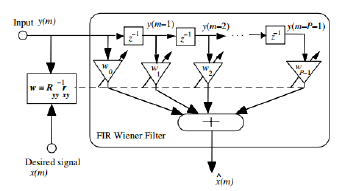
\includegraphics[width=0.55\textwidth]{Imagenes/Cap2/image014}
\end{center}
\begin{center}
\vskip -0.5cm
\caption{\small{Ilustración de la estructura de un filtro Wiener.}}
\label{fig:figura2.14}
{\small{Fuente: \cite{shubhra}}}
\end{center}
\end{figure}

Por otro lado, los filtros adaptativos confian en el uso de una fuente de ruido para eliminar el ruido de una señal recibida. Ordinariamente, es imprudente quitar ruido de una señal recibida, debido a que semejante operación pudiera producir resultados desastrosos, causando un incremento en la potencia promedio del ruido en la salida. Sin embargo, cuando se hacen previsiones apropiadas en el control del filtrado de la eliminación del ruido, es posible realizar un sistema superior de operación comparado al filtrado directo de la señal recibida.

\vskip 0.5cm
\begin{figure}[ht]
\begin{center}
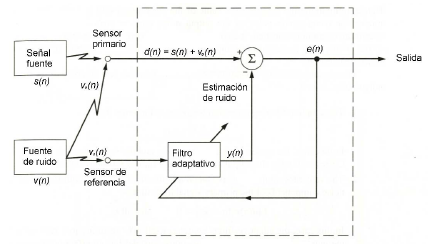
\includegraphics[width=0.7\textwidth]{Imagenes/Cap2/image015}
\end{center}
\begin{center}
\vskip -0.5cm
\caption{\small{Cancelador de ruido adaptativo.}}
\label{fig:figura2.15}
{\small{Fuente: \cite{walter}}}
\end{center}
\end{figure}

Básicamente, un cancelador de ruido adaptativo es un arreglo de doble entrada de lazo cerrado del sistema de realimentación como se ilustra en la Figura \ref{fig:figura2.15}, se derivan las dos entradas del sistema de un par de sensores: un sensor primario y un sensor de referencia (auxiliar). Específicamente, nosotros tenemos lo siguiente:

\begin{enumerate}
\item[1.]El sensor primario recibe una señal que lleva información \textit{s(n)} adulterada por un ruido aditivo \textit{$v_{0}(n)$}, como se muestra en la Ecuación \eqref{eq:ecuacion1}.

\begin{equation}
\label{eq:ecuacion1}
d(n) = s(n) + v_{0}(n)
\end{equation}

La señal $s(n)$ y el ruido $v_{0}(n)$ están sin correlación una de la otra, esto es:

\begin{equation}
\label{eq:ecuacion2}
E[s(n)v_{0}(n-k)] = 0 \hspace{1cm} \text{para todo \textit{k}}
\end{equation}

Donde $s(n)$ y $v_{0}(n)$ se suponen que son valores reales.

\item[2.]El sensor de referencia recibe un ruido $v_{1}(n)$ que no tiene correlación con la señal $s(n)$ pero si tiene correlación con el ruido $v_{0}(n)$, el cual es obtenido con el sensor primario junto a la señal que se desea recuperar; esto es:
\begin{equation}
\label{eq:ecuacion3}
E[s(n)v_{1}(n-k)] = 0 \hspace{1cm} \text{para todo \textit{k}}
\end{equation}
\vskip -1cm
\begin{equation}
\label{eq:ecuacion4}
E[v_{0}(n)v_{1}(n-k)] = p(k)
\end{equation}

Donde, la señal es un valor real y $p(k)$ es una correlación cruzada desconocida para el retardo $k$. La señal de referencia $v_{1}(n)$ es procesada por un filtro adaptativo para producir la salida:
\begin{equation}
\label{eq:ecuacion5}
y(n) = \sum_{k=0}^{M-1}\hat{w}_{k}(n)v_{1}(n-k)
\end{equation}

Donde, los $\hat{w}_{k}(n)$ son los valores de coeficientes (reales) ajustables del filtro adaptativo. La salida del filtro $y(n)$ es restada de la señal principal $d(n)$, conocida como la respuesta deseada para el filtro adaptativo. La señal de error se define por:
\begin{equation}
\label{eq:ecuacion6}
e(n) = d(n) - y(n)
\end{equation}

Así, sustituyendo la Ecuación \eqref{eq:ecuacion1} en la Ecuación \eqref{eq:ecuacion6}, se obtiene:
\begin{equation}
\label{eq:ecuacion7}
e(n) = s(n) + v_{0}(n) - y(n)
\end{equation}

La señal de error es la que se utiliza para ajustar los valores de coeficientes del filtro adaptativo y el lazo de control alrededor de las operaciones de filtrado y sustracción están relacionados. Note que la señal que lleva la información es cierta parte de la señal $e(n)$, como se indica en la Ecuación \eqref{eq:ecuacion7}.
\vskip 0.5cm
La señal de error $e(n)$ constituye la salida total del sistema. De la Ecuación \eqref{eq:ecuacion7} se puede ver, que la componente de ruido en la salida del sistema es $v_{0}(n) - y(n)$. Ahora comienza su labor el filtro adaptativo para minimizar el error cuadrático medio de la señal $e(n)$. La señal esencial $s(n)$ que lleva la información, no es afectada por el cancelador de ruido adaptativo.
\vskip 0.5cm
Así que, minimizando el error cuadrático medio de la señal $e(n)$ es equivalente a minimizar el error cuadrático medio del ruido de salida $v_{0}(n) - y(n)$. Con la señal $s(n)$ que permanece esencialmente constante, esto lleva a que la minimización del error cuadrático medio de la señal, es ciertamente la misma como la maximización de la razón señal a ruido de la salida del sistema.
\end{enumerate}

El uso efectivo del cancelador de ruido adaptativo requiere que se coloque el sensor de referencia en el campo de ruido del sensor primario.

\item[•]Estructura de los filtros adaptativos
\par
El algoritmo adaptativo debe disponer del error $e(n)$ para actualizar los coeficientes, ya que $e(n)$ permite definir las mejoras del filtro y determinar la forma en que han de modificarse dichos coeficientes. La eficiencia de un filtro adaptativo lineal depende de una serie de factores, como el tipo de filtro (IIR o FIR), la estructura del mismo (transversal, de celosía o sistólico), o la función de costo usada como criterio de adaptación (error cuadrático medio, mínimo error cuadrático, etc.).

Nuestro estudio se va a centrar en el filtro FIR (Respuesta Finita al Impulso) por varias razones:
\begin{enumerate}
\item[-]El error cuadrático medio para un filtro transversal es una función cuadrática de los pesos del filtro. La superficie de error es un paraboloide con sólo un mínimo, y por ello, la búsqueda del error cuadrático medio mínimo es relativamente sencilla.
\item[-]Dado que los coeficientes del filtro son limitados, se puede controlar fácilmente la estabilidad del filtro.
\item[-]Existen algoritmos para la actualización de los coeficientes que con filtros FIR son mucho más simples y eficientes.
\item[-]Las prestaciones de estos algoritmos son perfectamente conocidas en términos de convergencia y estabilidad.
\end{enumerate}
De los tres tipos de estructuras de filtro que se distinguen en el contexto de un filtro adaptativo lineal, vamos a conceder toda la atención al tipo transversal.
\begin{figure}[ht]
\begin{center}
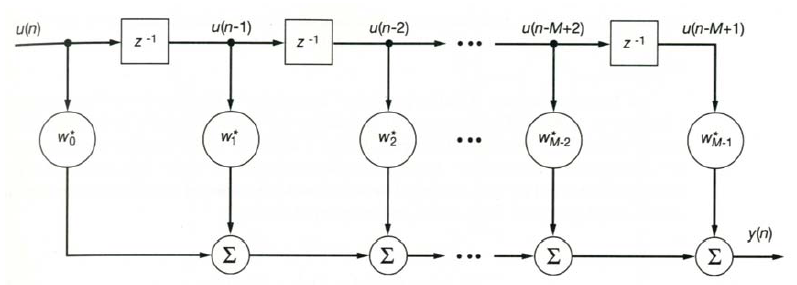
\includegraphics[width=0.48\textwidth]{Imagenes/Cap2/image016}
\end{center}
\begin{center}
\vskip -0.5cm
\caption{\small{Filtro transversal.}}
\label{fig:figura2.16}
{\small{Fuente: \cite{walter}}}
\end{center}
\end{figure}
\vskip -0.5cm
\newpage
Los filtros transversales, también llamados filtros directos de pesos retardados, consisten en tres elementos básicos, como se describió en la Figura \ref{fig:figura2.16}, primero los elementos de unidad de retardo, segundo el multiplicador, y tercero la sumatoria. El número de elementos de retardo usados en el filtro, mostrado como $M-1$ en la Figura \ref{fig:figura2.16}, determinan el filtro FIR, estos normalmente estan referidos al orden del filtro. Los elementos de retardo son identificados por el operador de la unidad de retraso $z^{-1}$. 
\vskip 0.5cm
En particular, cuando $z^{-1}$ opera en la entrada $u(n)$, la salida resultante es $u(n-1)$. El papel de cada multiplicador en el filtro es realizar el producto del valor de entrada por un coeficiente del filtro. Así un multiplicador conectado $k$ veces a entradas retardadas $u(n-k)$ produce la versión del escalar de que es el producto interno, $w^{*}_{k}u(n-k)$, donde $w_{k}$ va desde $k=1$ a $M$. El asterisco denota la conjugación compleja que asume la entrada y por consiguiente también los pesos actualizables son valores complejos. 
\vskip 0.5cm
El papel combinado de las sumatorias en el filtro es sumar los resultados de los productos individuales y producir una salida total del filtro. Para el filtro transversal descrito en la Figura \ref{fig:figura2.16}, la salida está dada de la siguiente manera:
\begin{equation}
\label{eq:ecuacion8}
y(n) = \sum_{k=0}^{M-1}W_{k} \cdot u(n-k)
\end{equation}
La ecuación es llamada sumatoria de convolución finita, en el sentido que la respuesta convoluciona el impulso de duración finita del filtro, $w^{*}_{n}$, con la entrada $u(n)$ del filtro, luego cada producto individual se suma para dar como resultado $y(n)$.
\vskip 0.5cm
La estructura transversal es la más sencilla de implementar, conduciendo a algoritmos igualmente sencillos. La estructura de celosía, presenta mejores propiedades, pues ofrece mayor robustez frente a errores de redondeo y una mayor eficiencia computacional. Sin embargo, aumenta la complejidad de los algoritmos. Por lo tanto, en el presente trabajo de tesis se adopta la primera estructura debido a su sencillez, pero aun así con buen desempeño.

\item[•]Aplicaciones de filtros adaptivos
\par
La habilidad de un filtro adaptativo es de operar de manera satisfactoria en un ambiente desconocido rastreando las variaciones estadísticas en el tiempo de una entrada, esto hace que los filtros adaptativos sean poderosos dispositivos para aplicaciones de procesado de señales y control. Es por eso que los filtros adaptativos han sido abundantemente aplicados en campos diversos tales como las comunicaciones, radar, sonar, sismología y la ingeniería biomédica. Aunque estas aplicaciones son de hecho bastante diferentes en naturaleza, no obstante, tienen un rasgo común básico: un vector de entrada y una respuesta deseada que se usan para calcular el error de estimación, que a su vez se usa para controlar los valores de un conjunto de coeficientes ajustables. 
\newpage
Los coeficientes ajustables pueden tomar la forma de pesos regulables, coeficientes de reflexión, parámetros de rotación o pesos sinápticos, dependiendo de la estructura del filtro empleada. Sin embargo, la diferencia esencial entre las varias aplicaciones de filtrado adaptativo comienza con la manera como se extrae la respuesta deseada. En este contexto, podemos distinguir cuatro clases básicas de aplicaciones de filtros adaptativos que ascienden a doce, como se describen en la Tabla \ref{table:tabla23}. En la sección anterior se describió el caso particular del cancelador de ruido, que es la que usaremos en esta tesis.

\begin{center}
\begin{table}[h!]
\centering
\vskip -0.2cm
\caption{\small{Aplicaciones de filtros adaptativos.}}
\label{table:tabla23}
\begin{tabular}{|c|c|}
\hline
{\small Clase de filtro adaptativo} & {\small Aplicación}\\
\hline
\multirow{2}{*}{\small I. Identificación}&{\small Identificación de Sistemas}\\&{\small Modelado de Capas Subterráneas}\\
\hline
\multirow{2}{*}{\small II. Modelado Inverso}&{\small Deconvolución Predictiva}\\&{\small Ecualización Adaptativa}\\& {\small Ecualización Ciega}\\
\hline
\multirow{2}{*}{\small III. Predicción}&{\small Codificación por Predicción Lineal (LPC)}\\&{\small Codificación Diferencial	Adaptativa (ADPCM)}\\&{\small Análisis Espectral Autorregresivo}\\&{\small Detección de Señal}\\
\hline
\multirow{2}{*}{\small IV. Cancelación de Interferencias}&{\small Cancelación Adaptativa de Ruido}\\&{\small Cancelación de Eco}\\&{\small Formas de haz Adaptativas}\\
\hline
\end{tabular}
\begin{center}
\vskip 0.2cm
{\small{Fuente: \cite{walter}}}
\end{center}
\end{table}
\end{center}

\item[•]Filtros adaptativos
\par
Tal y como vimos en la sección anterior, los filtros adaptativos son sistemas dinámicos lineales con estructura y parámetros variables o adaptables y tiene la propiedad para modificar los valores de sus parámetros, es decir su función de transferencia, durante el procesamiento de la señal de entrada genera una señal de salida que este sin componentes no deseados, ruido, degradación y también las señales de la interferencia.
\vskip 0.5cm
La Figura \ref{fig:figura2.18} muestra el concepto básico de un filtro adaptativo cual objetivo principal es filtrar la señal de entrada, $x(n)$, de tal una manera que se empareje a la señal deseada, el $d(n)$. La señal deseada, $d(n)$, se substrae de la señal filtrada, $y(n)$, para producir el error de la señal que a su vez maneja un algoritmo adaptivo que genera los coeficientes del filtro de una manera que minimiza el error de la señal. La adaptación ajusta las características del filtro a través de una interacción con el ambiente para alcanzar los valores deseados.

\begin{figure}[ht]
\begin{center}
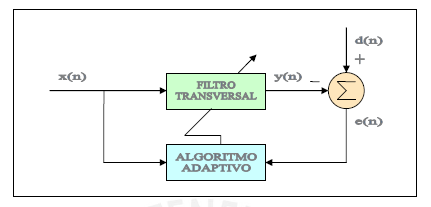
\includegraphics[width=0.5\textwidth]{Imagenes/Cap2/image018}
\end{center}
\begin{center}
\vskip -0.5cm
\caption{\small{Modelo de un filtro adaptativo.}}
\label{fig:figura2.18}
{\small{Fuente: \cite{simon}}}
\end{center}
\end{figure}

El filtro adaptativo ajusta sus coeficientes con un objetivo, garantizar la posible convergencia más rápida a los parámetros óptimos del punto de vista del criterio adoptado. La mayoría de algoritmos adaptivos significa modificaciones de los procedimientos iterativos normales para la solución del problema de minimización de la función de criterio en tiempo real. El más común de filtros adaptativos es el filtro transversal y es usado en, el algoritmo LMS (Mínimo Error Cuadrado Medio) y el algoritmo RLS (Mínimo Error Cuadrado Recursivo). Para lograr un buen desempeño del filtro adaptativo requiere el uso del mejor algoritmo adaptivo con baja complejidad computacional y un rango de convergencia rápido. A continuación, veremos algunos algoritmos adaptivos, pero nos centraremos más en los algoritmos LMS y NLMS.

\begin{enumerate}
\item[-]Algoritmo Least Mean Square (LMS)
\par
Un acercamiento muy sincero en el cancelamiento del ruido es el uso del algoritmo LMS desarrollado por Windrow y Hoff. Este algoritmo usa un descenso de la gradiente para estimar una variación del tiempo en la señal. El método de descenso de la gradiente encuentra un mínimo (si este existe), tomando los pasos en la dirección negativa de la gradiente y hace esto para ir ajustando los coeficientes del filtro para minimizar el error. La gradiente es un operador y se aplica para encontrar la divergencia de una función, que es el error con respecto en este caso al número de coeficientes. 
\vskip 0.5cm
El algoritmo LMS se ha aceptado por varios investigadores para la aplicación en el hardware debido a su estructura simple. Para llevarlo a cabo, las modificaciones tienen que ser hechas al algoritmo LMS original porque los bucles recursivos en la fórmula de actualización del filtro le impide ser un flujo lineal.
\vskip 0.5cm
La Ecuación \ref{eq:ecuacion9} muestra el detalle del algoritmo LMS, la evaluación de pesos:
\begin{equation}
\label{eq:ecuacion9}
w_{i}(n+1) = w_{i}(n) + \mu^{*}e(n)^{*}x(n-i)
\end{equation}

Salida filtrada:
\vskip -0.5cm
\begin{equation}
\label{eq:ecuacion10}
y(n) = \sum_{k=0}^{M-1}w_{i}(n)^{*}x(n-i)
\end{equation}
\vskip 0.5cm
La estimación del error, donde $e(n)$ es la salida deseada:
\vskip -1cm
\begin{equation}
\label{eq:ecuacion11}
e(n) = d(n) - y(n)
\end{equation}

Donde la salida del filtro adaptivo $y(n)$ y el error de la señal $e(n)$ son obtenidos por las Ecuaciones \eqref{eq:ecuacion10} y \eqref{eq:ecuacion11}, respectivamente. En estas ecuaciones $x(n)$ es el vector de la señal de entrada, y $w(n)$ es el vector de pesos del filtro adaptivo. 
\vskip 0.5cm
De estas ecuaciones, en cada iteración la información de la mayoría de los recientes valores son requeridos y el procedimiento reiterativo se inicia con una suposición inicial $w_{0}$. El $\mu$ es el tamaño del paso de adaptación que depende del poder de la densidad espectral de la entrada de referencia $x(n)$ y $M-1$ es el orden del filtro y controla la estabilidad y velocidad de la convergencia del algoritmo LMS.

\item[-]Algoritmo Normalized Least Mean Square (NLMS)
\par
La debilidad principal del LMS del tipo convencional radica en su complejidad seleccionando un valor conveniente para el parámetro de tamaño de paso que garantiza la estabilidad. Ante este inconveniente, fue propuesto el NLMS, controlando el factor de la convergencia del LMS a través de la modificación en un parámetro de tamaño de paso de tiempo variante. 
\vskip 0.5cm
El NLMS emplea un parámetro de tamaño de paso inconstante pensado a minimizar el error de salida instantáneamente el cual converge más rápidamente que el LMS convencional. El algoritmo LMS convencional experimenta en la gradiente problemas de amplificación de ruido cuando el factor de la convergencia $\mu$ es grande. La corrección se aplicó al vector de pesos $w(n)$ al $n+1$ de la iteración, es normalizada con respecto al cuadrado de la norma euclidiana del vector de entrada $x(n)$ a la iteración $n$. 
\vskip 0.5cm
Nosotros podemos expresar el algoritmo NLMS como un algoritmo de tamaño de paso de tiempo variante, calculando el factor de convergencia $\mu$ como en la Ecuación \eqref{eq:ecuacion12}.
\vskip -1cm
\begin{equation}
\label{eq:ecuacion12}
\mu(n) = \frac{\beta }{c+\left \| x(n) \right \|^{2}}
\end{equation}
\newpage
Dónde $\beta$ es la constante de adaptación del NLMS, que optimiza el rango de convergencia del algoritmo y debe satisfacer la condición $0< \beta <2$, y \textit{c} es el término constante para la normalización y siempre es menor que 1. Los pesos del filtro se actualizan por la Ecuación \eqref{eq:ecuacion13}
\vskip -1cm
\begin{equation}
\label{eq:ecuacion13}
w(n+1) = w(n) + \frac{\beta }{c+\left \| x(n) \right \|^{2}}e(n)x(n)
\end{equation}

En comparación al LMS, el NLMS tiene tamaño de paso variante que hace al NLMS para converger más rápidamente. Para sacar mejores aplicaciones se han desarrollado varias variantes del LMS, ver la Tabla \ref{table:tabla24}.

\begin{center}
\begin{table}[h!]
\centering
\vskip -0.2cm
\caption{\small{Variantes del algoritmo LMS.}}
\label{table:tabla24}
\begin{tabular}{c}
\begin{minipage}{.9\textwidth}
\begin{center}
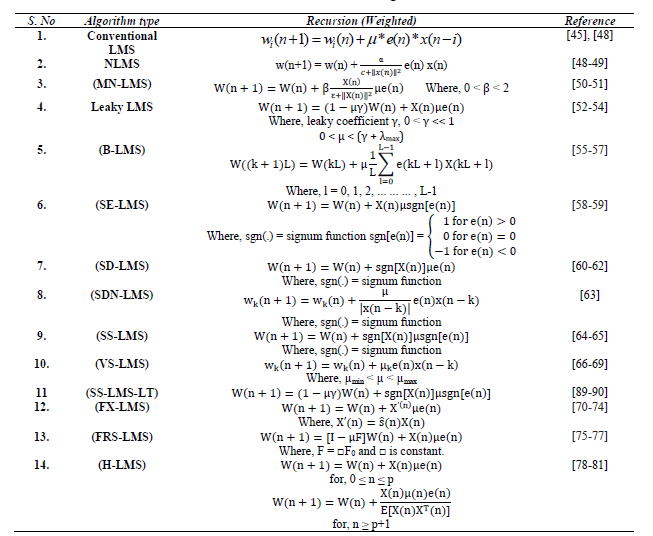
\includegraphics[width=0.7\textwidth]{Imagenes/Cap2/image019}
\end{center}
\end{minipage}
\end{tabular}
\begin{center}
\vskip 0.2cm
{\small{Fuente: \cite{shubhra}}}
\end{center}
\end{table}
\end{center}

\end{enumerate}

Además del LMS, NLMS y sus variantes, existen otros algoritmos adaptivos como el algoritmo RLS (Mínimo Error Cuadrado Recursivo), el algoritmo CMA (Adaptivo de Módulo Constante), el algoritmo DMI (Adaptivo de Inversión de Matriz Directa), los cuales pueden verse en \citep{shubhra}.
\vskip 0.5cm
\item[•]Convergencia
\par
Los coeficientes del filtro adaptativo se modifican constantemente hasta lograr que el error sea mínimo, es decir el algoritmo alcance la convergencia, dicho de otra manera, que la entrada se aproxime a la respuesta deseada. Para precisar lo que sucede, supongamos que el orden del filtro es $M=2$, es decir los coeficientes son de la forma $w(n)=[w1(n) w2(n)]$, siendo $\xi$ el error donde $\xi_{min}$ es el mínimo.
\vskip 0.5cm
Entonces el sistema se puede graficar en un espacio de tres dimensiones como se puede apreciar en la Figura \ref{fig:figura2.20}. Cuando empieza el algoritmo, el error es grande y a medida que el tiempo transcurre, los coeficientes van descendiendo por la curva a una velocidad relativa a $\mu$ hasta llegar a $\xi_{min}$. Pero se debe tener en cuenta que este proceso no sucede de una manera trunca, sino similar a una pelota deslizándose por la pared interna cuando llega al fondo, pasa de largo y vuelve a subir, pero con menor impulso y luego vuelve a bajar y así sucesivamente hasta detenerse en el fondo. El tiempo que se demore en detenerse en el fondo es el tiempo de convergencia y $w_{0}$ es el punto de convergencia.

\begin{figure}[ht]
\begin{center}
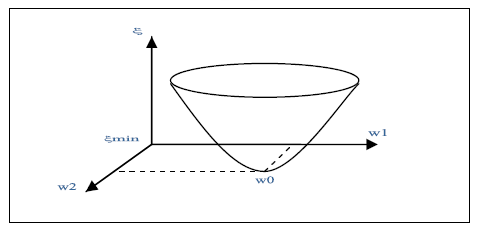
\includegraphics[width=0.4\textwidth]{Imagenes/Cap2/image020}
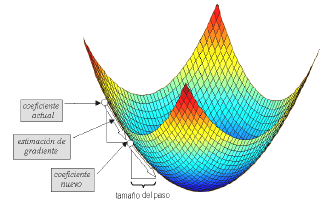
\includegraphics[width=0.4\textwidth]{Imagenes/Cap2/image021}
\end{center}
\begin{center}
\vskip -0.5cm
\caption{\small{Convergencia y error mínimo.}}
\label{fig:figura2.20}
{\small{Fuente: \cite{simon}}}
\end{center}
\end{figure}

En \citep{simon} se realizaron unas pruebas para obtener el mejor número de orden $M$ y tamaño de paso $\mu$ para el algoritmo LMS y el mejor número de orden $M$, la constante de adaptación $\beta$ y el término constante para la normalización $c$ para el algoritmo NLMS. Estas pruebas se realizaron con un micrófono primario ubicado a 2 metros de la fuente de ruido (equipo de sonido) y un segundo micrófono ubicado a 50 cm de la fuente de ruido. Se concluyo que cuando se utiliza un tamaño de paso grande ($\mu > 0.03$) el error en un determinado momento se eleva, el valor de $W$ se torna inestable, por lo cual se debe elegir un valor menor. 
\vskip 0.5cm
En la Figura \ref{fig:figura2.21} se puede apreciar como la energía se va reduciendo desde $M=32$ hasta $M=128$, pero luego vuelve a incrementarse como se dijo anteriormente. Entonces se puede concluir que el mejor valor de $M$ bordea el valor 128.
\newpage
\begin{figure}[ht]
\begin{center}
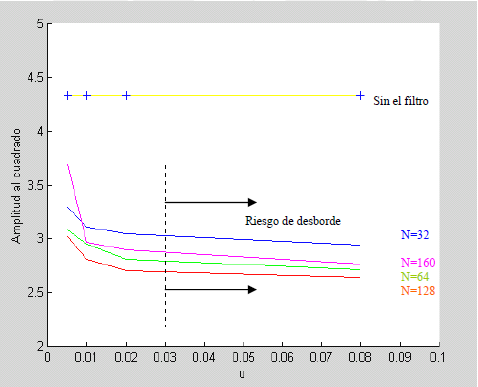
\includegraphics[width=0.45\textwidth]{Imagenes/Cap2/image022}
\end{center}
\begin{center}
\vskip -0.5cm
\caption{\small{Cuadrado promedio para diferentes valores de M y $\mu$ para el LMS.}}
\label{fig:figura2.21}
{\small{Fuente: \cite{simon}}}
\end{center}
\end{figure}

El error varía poco para un tamaño de paso entre 0.02 y 0.08 además debe ser menor a 0.03 para evitar el desborde, por lo que se eligió el valor de 0.02 que asegura la estabilidad del filtro y mantiene el error a un nivel aceptable, ver la Figura \ref{fig:figura2.22}.
\vskip 0.2cm
\begin{figure}[ht]
\begin{center}
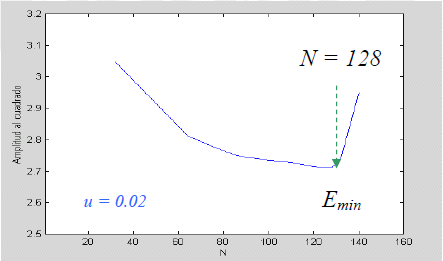
\includegraphics[width=0.45\textwidth]{Imagenes/Cap2/image023}
\end{center}
\begin{center}
\vskip -0.5cm
\caption{\small{Valor para el número de orden M con $\mu$\protect=0.02.}}
\label{fig:figura2.22}
{\small{Fuente: \cite{simon}}}
\end{center}
\end{figure}
\newpage
En la Figura \ref{fig:figura2.23} se puede apreciar que se obtuvo una buena eficiencia hasta 81dBC de ruido a 2m de distancia de los parlantes. Para el algoritmo NLMS se propuso los valores de $M =128$ al igual que el del LMS, con $\beta = 0.25$ y $c = 0.0001$.
\vskip 0.2cm
\begin{figure}[ht]
\begin{center}
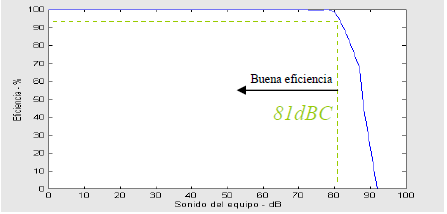
\includegraphics[width=0.5\textwidth]{Imagenes/Cap2/image024}
\end{center}
\begin{center}
\vskip -0.5cm
\caption{\small{Curva de eficiencia vs. sonido del equipo.}}
\label{fig:figura2.23}
{\small{Fuente: \cite{simon}}}
\end{center}
\end{figure}

Finalmente, esta etapa de eliminación de ruido estará conformada por dos submódulos, el primero será la eliminación de ruido donde evaluaremos los algoritmos LMS Y NLMS para luego elegir el que tenga un mejor comportamiento y el segundo es la normalización de la señal después de haber aplicado el filtro adaptativo, debido a que puede haber un aumento en el espectro de potencia. El proceso se puede ver en la Figura \ref{fig:figura2.24}.
\vskip 0.2cm
\begin{figure}[ht]
\begin{center}
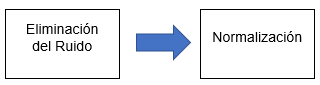
\includegraphics[width=0.3\textwidth]{Imagenes/Cap2/image025}
\end{center}
\begin{center}
\vskip -0.5cm
\caption{\small{Diagrama de eliminación de ruido y normalización.}}
\label{fig:figura2.24}
{\small{Fuente: \citep{eyra}}}
\end{center}
\end{figure}
\newpage
En \cite{mathematics} se muestra la formula para la normalización de la señal:\\
$[c, d]$ = rango de entrada mínimo y máximo.\\
$[m, n]$ = rango de salida mínimo y máximo.\\
Donde:
\begin{equation}
\label{eq:ecuacion14}
A = (m-n)/(c-d)
\end{equation}
\vskip -1cm
\begin{equation}
\label{eq:ecuacion15}
B = m - A*c
\end{equation}

Entonces para la señal de entrada $E(n)$ obtenemos la salida normalizada $S(n)$:
\begin{equation}
\label{eq:ecuacion16}
S(n) = A^{*}E(n) + B
\end{equation}
\end{enumerate}

\item[c)]Detección de inicio y fin de la señal de voz
\par
El problema de la localización del inicio y final de una muestra de voz en un fondo acústico de silencio es de vital importancia en muchas áreas del procesamiento de voz. En particular, el problema del reconocimiento de palabras está basado en la suposición de que se puede hallar la región de la muestra donde hay voz, para ser reconocida. 
\vskip 0.5cm
El poder determinar cuál es el inicio y el final de una palabra proporciona ciertas ventajas como, procesar menor cantidad de información, comparar únicamente los patrones de información y evitar confusiones a causa del ruido o señales de fondo.
\vskip 0.5cm
La tarea de separar la voz del espacio de silencio no es una tarea tan simple como puede parecer, esto puede suceder sólo en ambientes acústicos con tasa extremadamente alta de señal a ruido, por ejemplo, las cámaras a prueba de eco o de ruido, donde son hechas las grabaciones de alta calidad. Para dichos ambientes con alta relación señal a ruido, la energía de los sonidos de voz de más bajo nivel (fricativos débiles) excede la energía del ruido del fondo, por ende, una simple medición de la energía es suficiente para realizar las mediciones. 
\vskip 0.5cm
Sin embargo, dichas condiciones ideales de grabación no son prácticas para las aplicaciones del mundo real. Por ende, la simple medición de la energía se convierte en una condición necesaria más no suficiente para separar los fricativos débiles del fondo de silencio.
\vskip 0.5cm
Algunos de los problemas que se presentan en la detección son:
\begin{enumerate}
\item[-]Silencios contenidos dentro de las palabras que tienen fonemas plosivos (\textit{ej. /t/, /p/, /k/}) que pueden confundirse con un falso principio o fin. 
\item[-]Presencia de espurias de ruido que se pueden confundir con la señal. 
\item[-]Los fonemas fricativos (\textit{ej. /f/, /th/, /h/, etc.}), ya que tienen baja energía.
\item[-]Sonidos cortos (\textit{ej. /t/, /p/, /k/}).
\item[-]Detección de fonemas nasales al final de la palabra.
\item[-]Respiraciones del locutor, que pueden confundirse por su duración.
\item[-]Los micrófonos tienen resonancia después de pronunciar una palabra (sobre todo en vocales).
\item[-]Los niveles de ruido pueden confundirse con la señal de voz.
\end{enumerate}

En este trabajo de tesis se evaluará el algoritmo por función de energía y los algoritmos propuestos por Rabiner y Sambur, la expuesta en \citep{unam} la denominaremos \textit{Tipo 1} y la de \citep{rabiner} la denominaremos \textit{Tipo 2}, para la localización de los puntos de inicio y final de grabación de voz. Dicho algoritmo es muy útil y funciona muy bien en ambientes con una relación señal a ruido de al menos 30 dBC y está basado en dos mediciones de la voz, la energía de tiempo corto y la tasa de cruces por cero. Por último, se escogerá el que tenga mejor desempeño.

\begin{enumerate}
\item[•]Algoritmo por función de energía
\par
La señal digitalizada es escaneada y las zonas de silencio son removidas por medio del cálculo de energía en corto tiempo. En segmentos de 10 ms si la energía promedio es menor que un valor umbral, generalmente de valor 0.2 (proporcional a la energía promedio de la señal entera) es descartado, \cite{genoveva}. A continuación, se muestran las fórmulas que se utilizarán:

\begin{equation}
\label{eq:ecuacion17}
E_{n} = \sum_{m=0}^{N-1}\left | x[m] \right |^{2}
\end{equation}
\vskip -0.5cm
\begin{equation}
\label{eq:ecuacion18}
E_{avg} = \frac{1}{N}\sum_{k=1}^{N}\left | x[k] \right |^{2}
\end{equation}

Donde $E_{n}$ es la energía promedio de cada segmento y $E_{avg}$ es la energía promedio de la señal entera.

\item[•]Algoritmo de Rabiner y Sambur tipo 1
\par
Tanto la energía como la magnitud son útiles para distinguir segmentos sordos y sonoros en la señal de voz. Pero existen otras maneras para identificar segmentos sonoros, hay un método denominado \textit{cruces por cero y máximos}, se puede decir que una señal clasificada como ruido (la \textit{s} es un ruido de alta frecuencia) provoca en la amplitud un cambio de signo, de esta manera se pueden localizar consonantes fricativas.
\vskip 0.5cm
El algoritmo de Rabiner y Sambur combina la energía instantánea en una trama, con medidas de tasas de cruce por cero y confían en que un nivel alto de energía es el mejor estímulo para la detección. Se asume que la tasa de cruces por cero es bien distinta en zonas de voz con baja energía o de ruido de fondo y seria el punto adicional para determinar los límites de la voz.

\begin{enumerate}
\item[-]Energía de tiempo corto
\par
La energía de la voz $E(n)$, se define como la suma de las magnitudes de la voz al cuadrado en intervalos centrados de 10 ms, todo medido sobre el intervalo de medición, tal como se definió en la Ecuación \eqref{eq:ecuacion17}.
\vskip 0.5cm
En donde, $x(n)$ son las muestras de voz muestreadas a la frecuencia escogida. El escoger una ventana de 10 ms para el cálculo de la energía y el uso de la función de magnitud en lugar del cuadrado de la magnitud, se realizó porque puede causar un aumento en el espectro de la potencia, además así podemos aumentar la velocidad de computo, debido a que requerirá de una operación menos. La función de magnitud se define en la Ecuación \eqref{eq:ecuacion22}.

\item[-]Tasa de cruces por cero
\par
La tasa de cruces por cero de una grabación de voz $Z(n)$ se define como el número de cruces por cero en un intervalo de 10 ms. Aunque esta es altamente susceptible a ruido de 60 Hz, en la mayoría de los casos es una medida muy buena y razonable de la presencia o ausencia de silencio en la grabación.
\vskip 0.5cm
La principal suposición que se realiza al momento de aplicar este algoritmo es que los primeros 100 ms de grabación son silencio. Es por eso que, en este intervalo de tiempo, las estadísticas de silencio en el fondo de la grabación son medidas. Estas mediciones incluyen, la media de los valores de los datos digitalizados y la desviación estándar de la tasa de cruces por cero, así como la energía promedio.
\begin{equation}
\label{eq:ecuacion19}
Z(n) = \sum_{m=-\infty}^{\infty}\left | [x(m)] - [x(m-1)] \right |r(n-m)
\end{equation}
Donde:
\begin{equation}
\label{eq:ecuacion20}
\begin{split}
x(n)&= 1, x(n) \geq 0 \\ 
 &= -1, s(n) < 0
\end{split}
\end{equation}
Y
\begin{equation}
\label{eq:ecuacion21}
\begin{split}
r(n)&= \frac{1}{2N}, 0 \leq n \leq N-1 \\
 &= 0, \text{de otra manera}
\end{split}
\end{equation}
\vskip 0.2cm
\item[-]Algoritmo para la detección de inicio
\par
\begin{enumerate}
\item[1.]Por cada trama de 128 muestras, calcular las funciones: magnitud promedio $M_{n}$ y cruce por ceros $Z_{n}$, partiendo de las ecuaciones \eqref{eq:ecuacion17}, \eqref{eq:ecuacion19}, \eqref{eq:ecuacion20}, \eqref{eq:ecuacion21} estas funciones se definen a continuación: 
\begin{equation}
\label{eq:ecuacion22}
M_{n} = \sum_{m=0}^{N-1}\left | x[m] \right |
\end{equation}

\begin{equation}
\label{eq:ecuacion23}
Z_{n} = \frac{\sum\limits_{m=0}^{N-2}\left | sign(x[m+1]) - sign(x[m]) \right |}{2N}
\end{equation}
\item[2.]Para obtener las estadísticas del ruido ambiental se considera que las primeras diez ventanas son ruido, con lo cual se tiene:
\begin{equation}
\label{eq:ecuacion24}
\begin{split}
Ms_{n} &= \{M_{1},M_{2},...,M_{10}\}\\ 
Zs_{n} &= \{Z_{1},Z_{2},...,Z_{10}\}
\end{split}
\end{equation}
Donde $Ms_{n}$ es la magnitud del ruido y $Zs_{n}$ son los cruces por cero del ruido.
\item[3.]Calcular la media y la desviación estándar para las características del ruido y obtener los siguientes umbrales:
\begin{center}
\begin{table}[h!]
\centering
\caption{\small{Umbrales para la detección de inicio y fin de la señal de voz.}}
\label{table:tabla2.3}
\vskip 0.2cm
\begin{tabular}{|c|c|c|c|}
\hline
{\small\textbf{Umbral}} & {\small\textbf{Nombre del umbral}} & {\small\textbf{Valor}}  \\ 
\hline 
{\small $UmbSupEnrg$} & {\small Umbral Superior de Energía} & {\small $0.5^{*}max\{M_{n}\}$}  \\ 
\hline 
{\small $UmbInfEnrg$} & {\small Umbral Inferior de Energía} & {\small $\mu_{Ms} + 2^{*}\sigma_{Ms}$}  \\ 
\hline 
{\small $UmbCruCero$} & {\small Umbral de cruces por cero} & {\small $\mu_{Zs} + 2^{*}\sigma_{Zs}$}  \\ 
\hline
\end{tabular} 
\begin{center}
\vskip 0.2cm
{\small{Fuente: \cite{unam}}}
\end{center}
\end{table}
\end{center}

\vskip -1cm
\begin{equation}
\label{eq:ecuacion25}
\mu = \frac{\sum_{i}^{n}x_{i}}{N}
\end{equation}
\vskip -0.5cm
\begin{equation}
\label{eq:ecuacion26}
\sigma = \sqrt{\frac{\sum_{i}^{n}(x_{i} - \mu)^{2}}{N-1}}
\end{equation}
\vskip 0.5cm
Para el caso de $UmbSupEnrg$ se usa $M_{n}$ de la señal de voz (se considera a partir de las 10 tramas en adelante como señal de voz). En los siguientes dos casos, se usan los diez valores del ruido, obtenidos en el punto 2 para cada umbral. Recordar que es la media y la desviación estándar de la magnitud del ruido, así como la media y la desviación estándar del cruce por ceros del ruido.
\item[4.]Recorrer la función $M_{n}$ incrementando en una unidad a $n$ de 11 hasta que $M_{n} > UmbSupEnrg$. En este punto estamos garantizando presencia de señal. A este punto lo marcaremos como $I_{n}$.

\item[5.]Resulta lógico pensar que el inicio de la señal se encuentra en algún punto anterior a $I_{n}$, por lo que ahora recorremos la función $M_{n}$ desde $n = I_{n}$ hasta que $M_{n} < UmbInfEnrg$. Este punto lo marcaremos como $I_{e}$ y lo reconocemos tentativamente como el inicio de la señal, determinado por la función de magnitud.

\item[6.]Ahora disminuimos $n$, desde $n = I_{e}$ hasta $n = I_{e} \text{–} 25$ o en su defecto $n = 11$, verificando si se presenta alguna de las siguientes condiciones en la función de cruces por cero, ya que lo que ahora buscamos es la posibilidad de que un sonido no sonoro preceda a un sonido sonoro. Sí $Z_{n} < UmbCruCero$ significa que no encontramos alguna porción de la señal con aumento importante de frecuencia en 25 ventanas anteriores, por lo tanto, el inicio es $I_{e}$. Sí encontramos que $Z_{n} > UmbCruCero$ menos de tres veces seguidas significa que solo fue una espiga de ruido, el punto de inicio sigue siendo $I_{e}$.

\item[7.]Si encontramos que $Z_{n} > UmbCruCero$ al menos tres veces seguidas hemos encontrado un sonido no sonoro, entonces buscamos el punto $n$ para el cual $Z_{n} > UmbCruCero$ la primera de las más de tres veces, es decir, el punto para el cual la función $Z_{n}$ sobrepasa el umbral, indicando el comienzo del sonido no sonoro y desplazamos el inicio de la palabra de $I_{e}$ a $I_{z}$.
\end{enumerate}
\item[-]Algoritmo para la detección de fin
\par
Para la detección de fin de la señal de voz hacemos lo mismo, pero en sentido inverso a partir del punto (4) de la sección anterior, como si detectáramos un inicio con la señal invertida en el tiempo.
\end{enumerate}

\item[•]Algoritmo de Rabiner y Sambur tipo 2
\par
Al igual que el algoritmo anterior esta variante del algoritmo de Rabiner y Sambur también utiliza la energía de tiempo corto y la tasa de cruces por cero. La Figura \ref{fig:figura2.25} explica su funcionamiento, donde la señal se filtra en un ancho de banda entre 100 Hz y 4 KHz, con una frecuencia de muestreo de 8 KHz. De forma simple, el algoritmo de detección se basa en medidas de la energía cada 10 milisegundos (80 muestras a 8 KHz) según la fórmula.
\newpage
\begin{figure}[ht]
\begin{center}
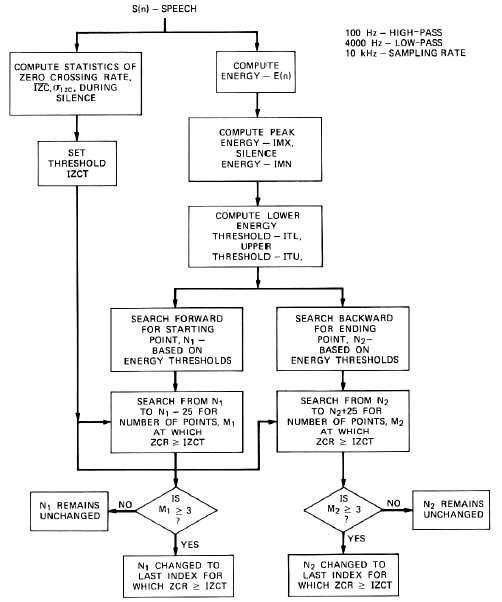
\includegraphics[width=0.6\textwidth]{Imagenes/Cap2/image026}
\end{center}
\begin{center}
\vskip -0.5cm
\caption{\small{Diagrama de flujo del algoritmo Rabiner y Sambur.}}
\label{fig:figura2.25}
{\small{Fuente: \cite{rabiner}}}
\end{center}
\end{figure}

Por otro lado, la tasa de cruces por cero $Z(n)$, también se calcula una vez cada trama de 10 milisegundos. El algoritmo supone que durante los 100 milisegundos primeros de la grabación no hay voz presente. Durante este periodo de silencio inicial se miden, la media $IZC$ (Cruce por Cero Integrado), y la desviación estándar \textit{IZC}, de la tasa de cruces por cero, la $IMX$ (Energía Máxima de Voz) y la $IMN$ (Energía Media del Ruido de fondo). Una vez obtenida la energía de toda la grabación se establecen los siguientes umbrales:

\begin{equation}
\label{eq:ecuacion27}
IZCT = MIN(IF,\overline{IZC} + 2\sigma _{IZC})
\end{equation}
\vskip -1.5cm
\begin{equation}
\label{eq:ecuacion28}
I1 = 0.03\cdot(IMX-IMN) + IMN
\end{equation}
\vskip -1.5cm
\begin{equation}
\label{eq:ecuacion29}
I2 = 4 \cdot IMN
\end{equation}
\vskip -1.5cm
\begin{equation}
\label{eq:ecuacion30}
ITL = MIN(I1,I2)
\end{equation}
\vskip -1.5cm
\begin{equation}
\label{eq:ecuacion31}
ITU = 5 \cdot ITL
\end{equation}

El umbral $IZCT$ tiene en cuenta el mínimo entre la tasa de cruces por cero promedios en una zona de silencio ($IZC$) más dos veces su desviación estándar y un umbral de tasa de cruces por cero $IF$, típicamente con valor 25. $I1$ simboliza la suma entre la $IMN$ (Energía Media del Ruido de fondo) y el 3\% de la diferencia entre el $IMX$ (\textit{Valor Máximo de la Energía de voz}) y la $IMN$ (Energía Media del Ruido de fondo). $I2$ es cuatro veces la $IMN$, $ITL$ el mínimo entre $I1$ e $I2$, y finalmente $ITU$, cinco veces $ITL$.
\vskip 0.5cm
En el detector sencillo que proponen Rabiner y Sambur, la decisión viene dada en función de una combinación de umbrales de energía y de tasa de cruces por cero. El diagrama de energía se puede visualizar en la Figura \ref{fig:figura2.26}.

\begin{figure}[ht]
\begin{center}
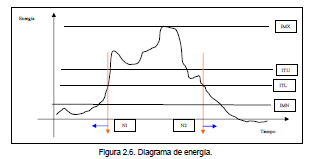
\includegraphics[width=0.55\textwidth]{Imagenes/Cap2/image027}
\end{center}
\begin{center}
\vskip -0.5cm
\caption{\small{Diagrama de energía.}}
\label{fig:figura2.26}
{\small{Fuente: \cite{varela}}}
\end{center}
\end{figure}

En este caso $IF$ es una constante de valor 25, ajustada manualmente, e $IMX$ es el pico de energía de la grabación incluyendo la voz principal. El comienzo del pulso, trama $N_{1}$, es el punto en el que la energía excede $ITL$:

\begin{enumerate}
\item[-]Si se supera $ITL$, estamos ante un posible pulso, pero todavía no se da ninguna confirmación debido a que podemos estar ante un pulso espurio.
\item[-]Una vez superado $ITL$, si además se supera $ITU$, ya se da la confirmación de pulso y se confirma también inicio de palabra. Se toma como inicio de pulso el instante de tiempo $N_{1}$ en el que supera $ITL$. Algo análogo ocurre con el final de pulso $N_{2}$.
\end{enumerate}
\vskip 0.5cm
\newpage
\begin{figure}[ht]
\begin{center}
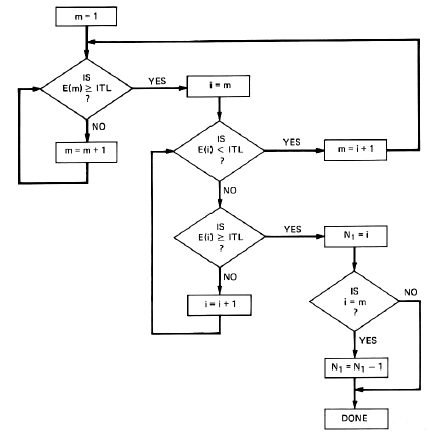
\includegraphics[width=0.35\textwidth]{Imagenes/Cap2/image028}
\end{center}
\begin{center}
\vskip -0.5cm
\caption{\small{Diagrama de flujo para la búsqueda del punto de inicio basado en la energía.}}
\label{fig:figura2.27}
{\small{Fuente: \cite{rabiner}}}
\end{center}

\begin{center}
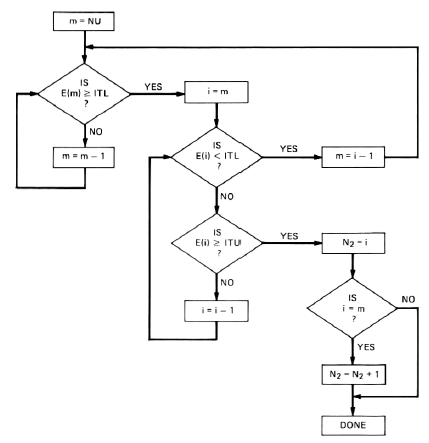
\includegraphics[width=0.35\textwidth]{Imagenes/Cap2/image029}
\end{center}
\begin{center}
\vskip -0.5cm
\caption{\small{Diagrama de flujo para la búsqueda del punto de fin basado en la energía.}}
\label{fig:figura2.28}
{\small{Fuente: \cite{rabiner}}}
\end{center}
\end{figure}

\newpage
Estos extremos son conservativos y se refina la localización de los extremos con la tasa de cruces por cero. El algoritmo examina desde $N_{1}$ hasta $N_{1}$ - $25$ (250 milisegundos) y si el número de veces que se excede el umbral $IZCT$ es tres o más, el punto de comienzo se retrasa al primer punto (en el tiempo) en el que excede el mencionado umbral. De lo contrario, el comienzo se mantiene en $N_{1}$. 
\vskip 0.5cm
De igual manera se opera en el intervalo comprendido entre $N_{2}$ y $N_{2} + 25$ (250 milisegundos). En cuanto a los umbrales de energía, se configuran los umbrales en función de lo robusto que se quiera ser ante espurios (por ejemplo, umbrales de energía $ITL$ e $ITU$ más altos). Es importante comentar que se pueden tratar los umbrales de energía que se quiera, tres, cuatro, en lugar de dos como en el caso del ejemplo ($ITL$ e $ITU$).
\vskip 0.2cm
\begin{figure}[ht]
\begin{center}
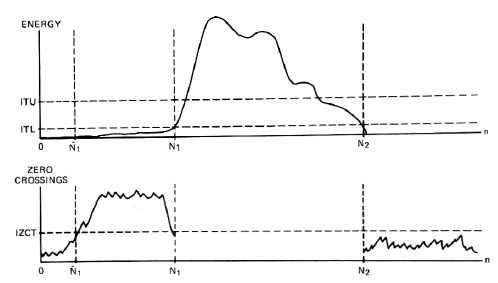
\includegraphics[width=0.45\textwidth]{Imagenes/Cap2/image030}
\end{center}
\begin{center}
\vskip -0.5cm
\caption{\small{Puntos de inicio y fin de la señal de voz.}}
\label{fig:figura2.29}
{\small{Fuente: \cite{rabiner}}}
\end{center}
\end{figure}
\end{enumerate}

\newpage
\item[d)]Filtro de preénfasis
\par
Consiste en aplicar un filtro digital pasa altas de primer orden a la señal. Las frecuencias altas de los formantes se enfatizan por dos razones, primero para que no se pierda información durante la segmentación, ya que la mayoría de la información está contenida en las frecuencias bajas, y segundo para remover la componente DC de la señal, aplanándola espectralmente, \cite{stephen}.

\begin{figure}[ht]
\begin{center}
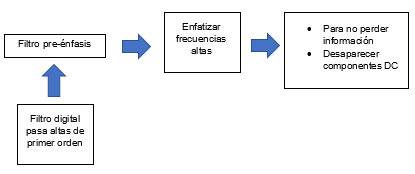
\includegraphics[width=0.45\textwidth]{Imagenes/Cap2/image031}
\end{center}
\begin{center}
\vskip -0.5cm
\caption{\small{Diagrama del filtro de preénfasis.}}
\label{fig:figura2.30}
{\small{Fuente: \cite{eyra}}}
\end{center}
\end{figure}
\vskip -0.5cm
Las componentes de alta frecuencia presentes en la señal de voz, normalmente tienen una amplitud menor con respecto a las componentes de baja frecuencia, debido a la atenuación que ocurre durante el mecanismo de producción de la voz, por lo que se necesita, realizar un preénfasis de las componentes de alta frecuencia, a fin de obtener una amplitud similar para todas las componentes, de tal manera que el espectro de la señal sea lo más plano posible. Este filtro FIR paso altas de primer orden, se encuentra definido por la siguiente ecuación, siendo $x(n)$ la señal de voz digitalizada:
\begin{equation}
\label{eq:ecuacion32}
x_{p} = x(n) - ax(n-1)\qquad
\begin{aligned}
& 0.9 \leq a \leq 1 \\
& n = 0,1,2,3,...,N_{x} - 1
\end{aligned}
\end{equation}
Donde $x_{p}(n)$ es la respuesta del filtro o la señal de voz con preénfasis y $\alpha$ es el parámetro de preénfasis. El valor más común para el parámetro de preénfasis es $\alpha = 0.95$, el cual proporciona un incremento de unos 20 dBC de amplificación para las componentes de alta frecuencia del espectro. No obstante, el valor exacto de este parámetro no es tan crítico. La Figura \ref{fig:figura2.31} muestra la magnitud de la respuesta en frecuencia de un filtro de preénfasis para una frecuencia de muestreo de $f_{s} = 8000 Hz$ y un parámetro de preénfasis $\alpha = 0.95$.
\vskip 0.2cm
\begin{figure}[ht]
\begin{center}
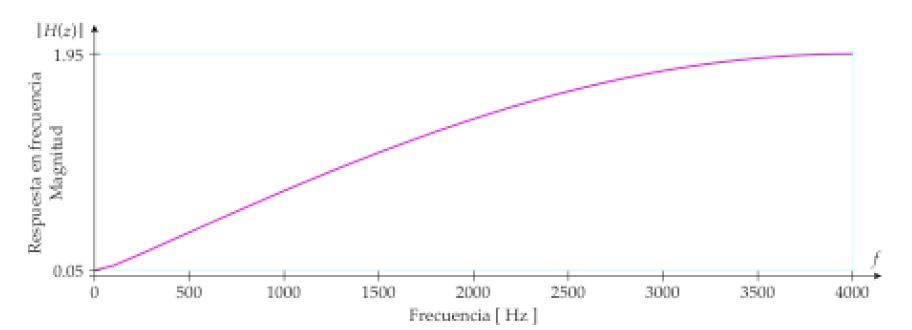
\includegraphics[width=0.5\textwidth]{Imagenes/Cap2/image032}
\end{center}
\begin{center}
\vskip -0.5cm
\caption{\small{Magnitud de la respuesta en frecuencia del filtro de preénfasis.}}
\label{fig:figura2.31}
{\small{Fuente: \cite{perez}}}
\end{center}
\end{figure}

\item[e)]Segmentación
\par
La segmentación consiste en cortar la señal de voz en segmentos de análisis y es asumida como estacionaria en estos. Durante este proceso los segmentos son guardados cada uno como la columna de una matriz, para el posterior procesamiento de la señal de voz.
\vskip 0.5cm
Para este proceso generalmente se emplea una ventana de Hamming de 30 ms que es aplicada a la señal de voz, enfatizada previamente con el filtro de preénfasis. Con un desplazamiento típico 10ms entre cada ventana.
\begin{figure}[ht]
\begin{center}
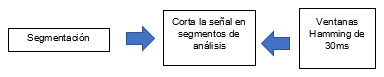
\includegraphics[width=0.6\textwidth]{Imagenes/Cap2/image033}
\end{center}
\begin{center}
\vskip -0.5cm
\caption{\small{Diagrama de segmentación, ventaneo y recorte de la señal de voz.}}
\label{fig:figura2.32}
{\small{Fuente: \citep{eyra}}}
\end{center}
\end{figure}

\begin{enumerate}
\item[•]División de tramas
\par
Los métodos tradicionales de análisis en frecuencia son bastante confiables para las señales estacionarias, pero este no es el caso de la señal de voz. Entonces, para poder emplear estas técnicas, resulta necesario dividir la señal en segmentos cortos o tramas para poder realizar un análisis en tiempo corto. Estas tramas pueden ser separadas y procesadas de manera individual, como si fueran segmentos cortos de un sonido sostenido con propiedades fijas. Este proceso se repite tantas veces como sea necesario hasta que se haya abarcado completamente la señal.
\vskip 0.5cm
Estos segmentos o tramas de análisis, son de longitud finita, consisten de $N$ muestras y normalmente se traslapan entre sí, teniendo $S$ muestras de desplazamiento o separación entre el inicio de una trama y la siguiente:
\begin{equation}
\label{eq:ecuacion33}
x_{l} = x(n + l \cdot S)\qquad
\begin{aligned}
& l = 0,1,2,3,...,L-1 \\
& n = 0,1,2,3,...,N-1
\end{aligned}
\end{equation}
En donde $x_{l}(n)$ es la l-ésima trama y $L$ es la cantidad o el número total de tramas presentes en la señal de voz $x(n)$. La Figura \ref{fig:figura2.33} ilustra la división en tramas con traslape de una señal de voz, para una separación entre tramas de $S = N/3$ muestras.
\begin{figure}[ht]
\begin{center}
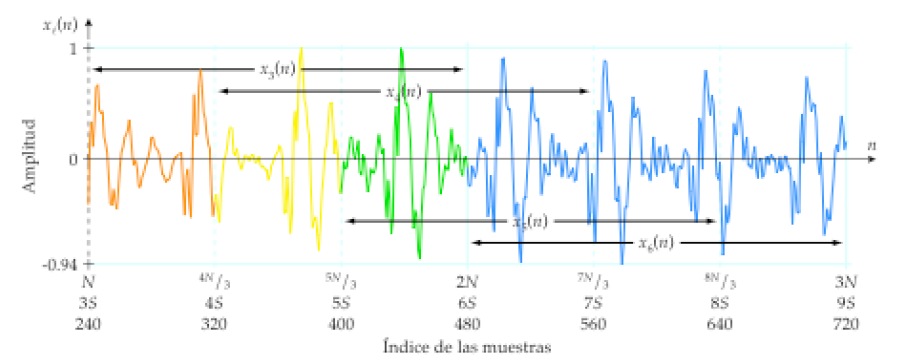
\includegraphics[width=0.75\textwidth]{Imagenes/Cap2/image034}
\end{center}
\begin{center}
\vskip -0.5cm
\caption{\small{División en tramas con traslape de una señal de voz.}}
\label{fig:figura2.33}
{\small{Fuente: \cite{perez}}}
\end{center}
\end{figure}

A partir de la figura anterior, se puede observar que la cantidad o el número total de tramas en la señal de voz es $L$, se puede calcular mediante la siguiente ecuación:
\begin{equation}
\label{eq:ecuacion34}
L = \frac{N_{x} - N}{S} + 1
\end{equation}
Si $N>S$, entonces sí ocurre el traslape y $N \text{-} S$ muestras al final de las tramas son duplicadas al inicio de la siguiente trama. Entre mayor sea el traslape, la correlación entre las tramas adyacentes también será mayor y los cambios serán más suaves. Por otra parte, si $N < S$, entonces no hay traslape, pero además algunas porciones de la señal de voz se perderán, ya que no aparecerán en ninguna de las tramas. Por lo tanto, esta última situación resulta inaceptable en cualquier tipo de procesamiento de voz.
\vskip 0.5cm
Entonces, la señal de voz se divide en $L$ tramas para su análisis. Cada una de éstas se compone por $N$ muestras con $S$ muestras de separación entre tramas adyacentes. Sin embargo, para no perder las propiedades dinámicas o variantes en el tiempo de la señal de voz, es necesario volver a calcular otros coeficientes para la siguiente trama.

\item[•]Ponderado por la ventana de Hamming
\par
Primero demos un vistazo a la más simple de las ventanas, la cual tiene una forma rectangular y se define como:
\begin{equation}
\label{eq:ecuacion35}
%
w(n) = 
\begin{cases}
0 & \text{para $n < 0$} \\ 
1 & \text{para $0 \leq  n \leq  N-1$} \\ 
0 & \text{para $n > N-1$} 
\end{cases}
%
\end{equation}
Esta ventana rectangular se usa de manera implícita cuando se extrae una trama de $N$ muestras a partir de una señal de voz:

\newpage
\begin{figure}[ht]
\begin{center}
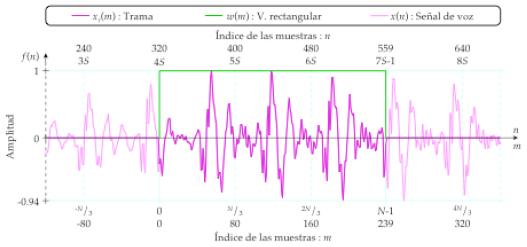
\includegraphics[width=0.75\textwidth]{Imagenes/Cap2/image035}
\end{center}
\begin{center}
\vskip -0.5cm
\caption{\small{Extracción de una trama mediante una ventana rectangular.}}
\label{fig:figura2.34}
{\small{Fuente: \cite{perez}}}
\end{center}
\end{figure}

Sin embargo, la presencia de ésta ventana ocasiona la distorsión del espectro de la señal de voz, pero si se pondera la trama por una ventana con la forma adecuada, entonces se puede reducir la distorsión en la frecuencia, aunque se deforme la señal en el tiempo. En el reconocimiento de voz, la ventana que más se utiliza es la de Hamming:
\begin{equation}
\label{eq:ecuacion36}
%
w(n) = 
\begin{cases}
0 & \text{para $n < 0$} \\ 
0.54 - 0.46cos(\frac{2\pi n}{N-1}) & \text{para $0 \leq  n \leq  N-1$} \\ 
0 & \text{para $n > N-1$} 
\end{cases}
%
\end{equation}
La Figura \ref{fig:figura2.35} es la representación gráfica de la ventana de Hamming, la cual tiene valores que decaen suavemente hacia cero, aunque en los extremos, tiene una transición abrupta para el primer y el último valor de la ventana, los que son iguales a 0.08.

\newpage
\begin{figure}[ht]
\begin{center}
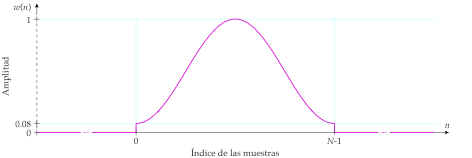
\includegraphics[width=0.6\textwidth]{Imagenes/Cap2/image036}
\end{center}
\begin{center}
\vskip -0.5cm
\caption{\small{Ventana de Hamming.}}
\label{fig:figura2.35}
{\small{Fuente: \cite{perez}}}
\end{center}
\end{figure}
El segmento o la trama ponderada $x_{w}(n)$ se obtiene mediante el producto de cada una de las muestras de la trama de análisis $x_{l}(n)$ por el peso correspondiente de la ventana de Hamming $w(n)$:
\begin{equation}
\label{eq:ecuacion37}
\begin{aligned}
& x_{w}(n) = x_{l}(n) \cdot w(n) \\
& x_{w}(n) = x_{l}(n) \cdot \left [ 0.54 - 0.46cos\left ( \frac{2 \pi n}{N-1} \right ) \right ]
\end{aligned}
\qquad
n = 0,1,2,3,...,N-1
\end{equation}
\vskip 0.5cm
El ponderado de la trama de análisis contribuye a minimizar las discontinuidades al inicio y al final de las tramas, al atenuar los valores en los extremos. De otro modo la disparidad entre la primera y la última muestra de la trama ocasionaría algunos efectos indeseables en los valores del espectro en frecuencia. No obstante, si las muestras que se encuentran cerca de los extremos de la trama describen algún evento significativo de corta duración, entonces este evento prácticamente no afecta a la trama, dado que recibe un ponderado bajo. Así que normalmente, las tramas se traslapan para asegurar que todos estos eventos se tomen en cuenta al ser cubiertos en las tramas adyacentes.

\item[•]Longitud de trama o tamaño de ventana
\par
La selección de la longitud de la trama $N$ es una consideración muy importante, pues por lo general, el trabajo de computo requerido durante el análisis es proporcional a esta, por lo que resulta ventajoso mantenerla tan pequeña como sea posible. Sin embargo, se deben abarcar varios periodos del tono fundamental (pitch) para asegurar que los resultados sean confiables. Además, debido al ponderado, la longitud de la trama debe ser lo suficientemente larga como para que los efectos de atenuación de la ventana de Hamming no afecten seriamente los resultados. 
\vskip 0.5cm
Adicionalmente, la longitud o la duración de la trama se determina mediante un compromiso entre las resoluciones en el tiempo y en la frecuencia, ya que la longitud de la trama es proporcional a la resolución en frecuencia, pero inversamente proporcional a la resolución en el tiempo. De manera similar, el traslape es proporcional al número de tramas en la señal de voz, pero también es proporcional a la correlación de las tramas subsecuentes. Por lo tanto, se debe buscar un balance o compromiso entre estas características contrapuestas.
\vskip 0.5cm
Una manera para determinar $V$ (longitud de la trama N), es haciendo el producto de la duración de la trama $T$ por la frecuencia de muestreo $f_{s}$ de la señal de voz:
\begin{equation}
\label{eq:ecuacion38}
V = (T:f_{s})_{int}
\end{equation}
No obstante, como el número de muestras por trama $N$ debe ser un valor entero, se debe redondear o truncar el resultado. El número de muestras de separación entre tramas adyacentes $S$, generalmente se selecciona de tal manera que se obtenga una tasa de 100 tramas por segundo ($Fps = 100$), es decir una trama cada 10 ms.
\begin{equation}
\label{eq:ecuacion39}
Fps = \frac{f_{s}}{S} \hspace{1cm} \Rightarrow \hspace{1cm} S = \frac{f_{s}}{100}
\end{equation}
Los valores típicos de $V$ son de 10 a 30 ms. Las ventanas cortas han sido propuestas para estimar los parámetros del tracto vocal que varían rápidamente, mientras que las ventanas largas se usan para estimar la frecuencia del tono fundamental (pitch). Las tramas de 20 a 30 ms de duración generalmente tienen una buena relación entre ambas resoluciones, \cite{eyra}.
\vskip 0.5cm
Hasta aquí hemos visto todos los componentes que conforman el módulo de preprocesamiento, a continuación, veremos el módulo de entrenamiento.
\end{enumerate}
\end{enumerate}

\newpage
\subsubsection{Entrenamiento}
Para el entrenamiento se deben capturar diversas palabras recortadas por medio del módulo de preprocesamiento, mismas que representan las diferentes repeticiones. A partir de estas repeticiones se obtiene un conjunto de centroides que son almacenados en la memoria. Para poder obtener estos centroides los valores numéricos obtenidos del preprocesamiento deben pasar por un algoritmo de extracción de características.
\begin{enumerate}
\item[a)]Extracción de características
\par
Es el proceso mediante el cual, dado un conjunto de datos se desea obtener otro conjunto de datos resumidos, pero que contengan solo la información necesaria de los datos de entrada. Una buena técnica de extracción de características garantiza que dichos datos obtenidos son únicos para una determinada entrada, es decir que para dos señales de entrada diferentes, se obtiene dos conjuntos de características diferentes, \cite{claudio}.
\vskip 0.5cm
Sin embargo, obtener características plenamente diferentes involucra que todas las señales sean diferentes, así se traten de dos palabras iguales, pero con diversas tonalidades y velocidades. Por lo tanto, la obtención de características debe de asegurarme, que en ambas señales existen características que son propias para ambas. De esta manera podemos obtener un grado de similaridad adecuado para el reconocimiento de la señal de voz.
\vskip 0.5cm
Entre muchas técnicas de extracción de características, podemos mencionar las siguientes:
\begin{enumerate}
\item[-]Algoritmo de características Fonético Acústicas
\item[-]Algoritmo basado en la Transformada de Fourier
\item[-]Codificación Predictiva Lineal (LPC)
\item[-]Coeficientes Cepstrales en Escala Mel (MFCC)
\item[-]Predicción Perceptual Lineal (PLP)
\item[-]Algoritmo basado en Wavelet.
\end{enumerate}

En \citep{unam}, se hace un análisis comparativo entre los algoritmos LPC, MFCC y PLP teniendo como resultado al MFCC como mejor algoritmo de extracción de características, ver la Figura \ref{fig:figura2.36}. En \citep{orlando}, se realiza una evaluación y comparación entre los Wavelets y los MFCC, resultando también a los MFCC con mejor desempeño, pero si bien tienen la misma complejidad computacional el tiempo de ejecución de los Wavelets es menor.

\newpage
\begin{figure}[ht]
\begin{center}
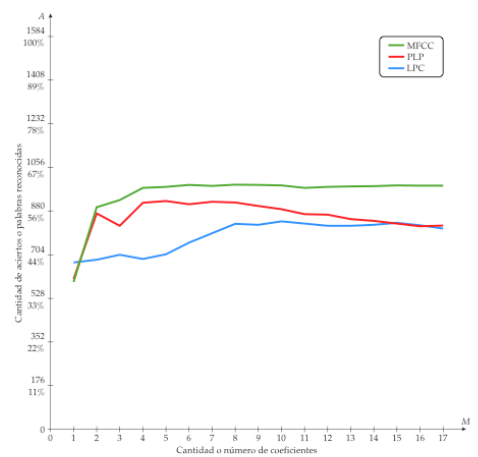
\includegraphics[width=0.55\textwidth]{Imagenes/Cap2/image037}
\end{center}
\begin{center}
\vskip -0.5cm
\caption{\small{Comparación de la variación en el reconocimiento entre LPC, MFCC Y PLP.}}
\label{fig:figura2.36}
{\small{Fuente: \cite{unam}}}
\end{center}
\end{figure}

Para este trabajo de Tesis teniendo lo anterior como antecedentes, hemos optado por la técnica MFCC (Coeficientes Cepstrales en la Frecuencia de Mel). La Figura \ref{fig:figura2.37} muestra el proceso del MFCC y como al final se retornan los cepstrum.

\begin{figure}[ht]
\begin{center}
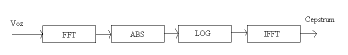
\includegraphics[width=0.5\textwidth]{Imagenes/Cap2/image038}
\end{center}
\begin{center}
\vskip -0.5cm
\caption{\small{Proceso de extracción de características con MFCC.}}
\label{fig:figura2.37}
{\small{Fuente: \cite{rabiner}}}
\end{center}
\end{figure}

\newpage
\item[b)]Codificación o análisis Mel cepstral
\par
En 1980 Davis y Mermelstein propusieron un nuevo tipo de representación del cepstrum, en el cual combinaron sus ventajas con los conocimientos de la percepción no lineal de la frecuencia en el sistema auditivo humano, tomando como base los estudios realizados por Zwicker en 1961. En este método de análisis, se utiliza la parte real del cepstrum, pero con una transformación no lineal de la frecuencia, pasando de la escala en Hertz a la escala de frecuencia Mel. Por eso, a estos coeficientes se les ha denominado como los Coeficientes Cepstral en la Frecuencia Mel o MFCC, \cite{eyra}.
\vskip 0.5cm
La mayor parte de los sistemas han estado convergiendo hacia el uso de estos vectores, que se obtienen a partir de un procesamiento de la señal de voz empleando un banco de filtros que ha sido diseñado tomando en cuenta algunas propiedades de la percepción del sonido en el sistema auditivo humano, con lo que se busca imitar su comportamiento.
\vskip 0.5cm
A continuación, se describe un procedimiento para obtener los coeficientes MFCC. La Figura \ref{fig:figura2.38} muestra el diagrama de bloques para este procedimiento. Los bloques muestran las operaciones necesarias y a la izquierda de éstos se muestran los parámetros de entrada requeridos en cada paso. A partir del cuarto bloque, el ponderado por la ventana de Hamming, las operaciones se realizan sobre las tramas de la señal de voz. La consiguiente reducción en el número de parámetros para cada trama se ilustra mediante la cantidad de flechas.

\newpage
\begin{figure}[ht]
\begin{center}
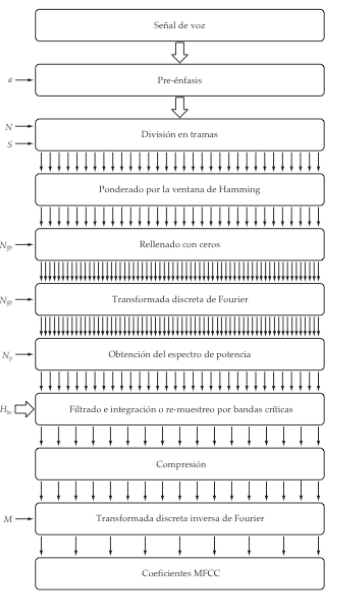
\includegraphics[width=0.4\textwidth]{Imagenes/Cap2/image039}
\end{center}
\begin{center}
\vskip -0.5cm
\caption{\small{Procedimiento para la obtención de los coeficientes MFCC.}}
\label{fig:figura2.38}
{\small{Fuente: \cite{eyra}}}
\end{center}
\end{figure}

Las etapas preénfasis, división de tramas y ponderado por la ventana de Hamming ya las vimos en la etapa de preprocesamiento, por lo que solamente veremos las etapas restantes.

\newpage
\begin{enumerate}
\item[•]Transformada discreta de Fourier
\par
El espectro en frecuencia de una señal discreta se puede estimar mediante DFT (Transformada Discreta de Fourier):
\begin{equation}
\label{eq:ecuacion40}
X(k) = \sum_{n=0}^{N-1}x(n)e^{-j\frac{2\pi nk}{N}}
\end{equation}
Esta transformada proporciona un conjunto de $N$ valores en el dominio de la frecuencia, en donde $X(k)$ es la transformada discreta de Fourier en el dominio de la frecuencia, de la señal discreta $x(n)$ en el dominio del tiempo. Sin embargo, en la práctica, la transformada discreta de Fourier se calcula de una manera mucho más eficiente mediante FFT (Transformada Rápida de Fourier).

\item[•]Rellenado con ceros
\par
Para facilitar el uso de la transformada rápida de Fourier, la longitud de la trama $N$ debería de ser igual al número de puntos para la transformada rápida de Fourier $N_{fft}$, un número que debe ser igual a la potencia de dos más próxima:
\begin{equation}
\label{eq:ecuacion41}
N_{fft} = 2^{[log_{2}(N)]_{int}}
\end{equation}
Pero si no se cumple con esta condición, entonces se puede rellenar con ceros, es decir, añadir las muestras nulas que hagan falta.
\vskip 0.5cm
\begin{equation}
\label{eq:ecuacion42}
x_{zp}(n)= \left\{ \begin{array}{lcl}
x_{w}(n) & \mbox{ para } & n = 0,1,2,3,...,N-1 \\
& & \\
0 & \mbox{ para } & n = N,N+1,...,N_{fft} - 1
\end{array}
\right.
\end{equation}
\vskip 0.5cm
A partir de la Ecuación \eqref{eq:ecuacion40} de la transformada discreta de Fourier se tiene:
\begin{equation}
\label{eq:ecuacion43}
X(k) = \sum_{n=0}^{N_{fft}-1}x(n)e^{-j\frac{2\pi nk}{N_{fft}}}
\end{equation}
Se puede apreciar que el agregar valores nulos a $x(n)$ no afecta significativamente la sumatoria para cualquier $X(k)$. Sin embargo, la longitud aumentada de la trama $N_{fft}$ solamente proporciona una mejor descripción de la transformada discreta de Fourier, pues no incrementa la resolución en frecuencia, pues este es el único propósito de la longitud de la trama $N$.

\item[•]\textbf{Obtención del espectro de frecuencia}
\par
El espectro en frecuencia de una trama de análisis se obtiene mediante el algoritmo FFT (Transformada Rápida de Fourier):
\begin{equation}
\label{eq:ecuacion44}
X(k) = \mathbf{FFT}\{ x_{zp}(n), N_{fft} \}
\qquad
\begin{aligned}
& k = 0,1,2,3,...,N_{fft}-1 \\
& n = 0,1,2,3,...,N_{fft}-1
\end{aligned}
\end{equation}
Dado que la señal de voz $x(n)$ es una secuencia de números reales, $X(k)$ y $X(N - k)$ son conjugados complejos. Puesto que la magnitud de los conjugados complejos es igual, el espectro en frecuencia resultante tiene una simetría par con respecto a la mitad de la frecuencia de muestreo, es decir, que la magnitud de la mitad superior del espectro es un reflejo de la mitad inferior.

\item[•]Obtención del espectro de potencia
\par
Ahora bien, no importa tanto la respuesta en frecuencia, sino la envolvente de la respuesta en frecuencia. Las características del tracto vocal se pueden estimar mediante el espectro de potencia $P(k)$ que se calcula como la magnitud del espectro al cuadrado o la suma de los cuadrados de la parte real e imaginaria del espectro:
\begin{equation}
\label{eq:ecuacion45}
\begin{aligned}
& P(k) = \left | X(k) \right |^{2} \\
& P(k) = \mathbf{real}[X(k)]^{2} + \mathbf{imag}[X(k)]^{2}
\end{aligned}
\qquad
k = 0,1,2,3,...,N_{fft}-1
\end{equation}
El espectro de potencia se compone de valores reales, enfatiza los picos en el espectro y conserva la simetría par del espectro en frecuencia. Por lo tanto, normalmente solamente se ocupa la mitad inferior del espectro, es decir los primeros $N_{p}$ valores:
\begin{equation}
\label{eq:ecuacion46}
\begin{aligned}
& N_{p} = 0.5N_{fft} \\
& P(k) = \mathbf{real}[X(k)]^{2} + \mathbf{imag}[X(k)]^{2} \qquad k = 0,1,2,3,...,N_{p}
\end{aligned}
\end{equation}
Hay que destacar que el espectro de potencia solamente proporciona información acerca de la magnitud, pues la información relacionada con la fase se descarta. Esto es consistente con el hecho de que la fase no aporta ninguna información que resulte útil. De hecho, se ha comprobado experimentalmente que la percepción de una señal reconstruida con una fase distinta es prácticamente indistinguible de la señal original, esto si se mantiene la continuidad secuencial de la fase entre las tramas.

\item[•]Filtrado e integración o remuestreo por bandas criticas
\par
El análisis espectral revela aquellas características de la señal de voz que son consecuencia directa de la configuración del tracto vocal. Asimismo, estas características de la voz por lo general se obtienen como las respuestas o salidas de un banco de filtros.
\vskip 0.5cm
Ahora bien, se ha encontrado que la percepción de una frecuencia en particular por parte del sistema auditivo humano está influenciada por la energía dentro de una banda crítica de frecuencias a su alrededor. En la psicoacústica, a esta propiedad se le conoce como la resolución espectral por bandas críticas.
\vskip 0.5cm
Un método muy utilizado para implementar estos bancos, consiste en efectuar el filtrado directamente en el dominio de la transformada discreta de Fourier. Los filtros simplemente son versiones desplazadas en la escala de frecuencia de alguna ventana. 
\vskip 0.5cm
Estas ventanas no están equiespaciadas en la escala de frecuencia en Hertz, de hecho se utiliza otra escala no lineal (logarítmica) para conseguir una mejor relación entre las resoluciones en el tiempo y en la frecuencia, pues los filtros de banda angosta para baja frecuencia hacen posible la detección de las frecuencias del tono fundamental (pitch), pero el incremento en el ancho de banda de los filtros para alta frecuencia permiten una mejor resolución en el tiempo, con la que se pueden detectar las plosivas. Además, la parte del espectro que se encuentra por debajo de 1000 Hz se procesa por una mayor cantidad de filtros, pues ésta contiene más información.
\vskip 0.5cm
La respuesta en frecuencia del banco de filtros simula el proceso de percepción que tiene lugar dentro del oído interno del humano, por eso a este proceso de filtrado también se le denomina como ponderado perceptual. La Figura \ref{fig:figura2.39} muestra la estructura general de estos bancos de filtros perceptuales, en donde $BC$ es la cantidad o el número de filtros o bandas críticas en el banco. 
\begin{figure}[H]
\begin{center}
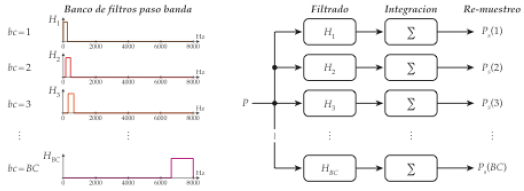
\includegraphics[width=0.5\textwidth]{Imagenes/Cap2/image040}
\end{center}
\begin{center}
\vskip -0.5cm
\caption{\small{Estructura general de los bancos de filtros perceptuales.}}
\label{fig:figura2.39}
{\small{Fuente: \cite{eyra}}}
\end{center}
\end{figure}
\vskip -0.5cm
Entonces, al integrar las salidas individuales de los filtros, se obtiene una muestra por cada una de las bandas críticas, por lo que el espectro es remuestreado a determinados rangos de frecuencia, proporcionando así, una compresión o reducción en el número de parámetros. 
\vskip 0.5cm
El efecto neto de esta etapa es reducir la sensibilidad del espectro a la frecuencia, particularmente para las altas frecuencias, las cuales de alguna manera son enfatizadas debido al ancho de banda más amplio de los filtros del banco.

\item[•]Cambio de la escala de frecuencia
\par
Existen muchas formas diferentes para las ventanas que se pueden emplear en los bancos de filtros, pero todas estas se basan en alguna escala de frecuencia que se considera aproximadamente lineal para frecuencias menores de 1000 Hz, pero para frecuencias mayores que ésta, presenta un comportamiento no lineal (logarítmico).
\vskip 0.5cm
Este cambio en la escala de frecuencia en inglés se denomina \textit{frequency warping}, es decir, que se realiza un arqueado o una transformación de la escala de frecuencia en Hertz, a otra escala de frecuencia que exhibe un comportamiento logarítmico. Las escalas Mel, que es la que usaremos en esta tesis, y Bark son dos ejemplos, puesto que están basadas en datos experimentales de la percepción humana, existen varias aproximaciones que se pueden usar para estas. A continuación, explicaremos en que consiste la escala de Mel.

\item[•]Escala Mel
\par
La escala Mel fue propuesta por Stevens, Volksman y Newmann en 1940. Un Mel es una unidad de medición de la frecuencia o del tono percibido, esta no corresponde de manera lineal a la frecuencia real del tono. Se designó como punto inicial de referencia, que una frecuencia de 1000 Hz también es de 1000 Mels. 
\vskip 0.5cm
Los observadores juzgan tonos espaciados exponencialmente como tonos equiespaciados. De esta manera fue posible determinar un mapeo entre la escala de la frecuencia real (Hertz) y la escala de la frecuencia percibida (Mels).
\vskip 0.5cm
La siguiente ecuación proporciona una equivalencia entre la escala logarítmica de la frecuencia Mel $f_{mel}$ con respecto a la escala de frecuencia en Hertz $f_{Hz}$:
\begin{equation}
\label{eq:ecuacion47}
f_{mel}(f_{Hz}) = \frac{1000}{\mathbf{Ln}(2)}\mathbf{Ln}\left ( 1 + \frac{f_{Hz}}{1000} \right )
\end{equation}
No obstante, se acostumbra utilizar otra función de aproximación para realizar la transformación no lineal de la frecuencia en Hertz a la escala de frecuencia Mel:
\begin{equation}
\label{eq:ecuacion48}
f_{mel}(f_{Hz}) = 1125\mathbf{Ln}\left ( 1 + \frac{f_{Hz}}{700} \right )
\end{equation}
La Figura \ref{fig:figura2.40} muestra la representación gráfica de la ecuación anterior, en donde se puede apreciar el arqueado de la frecuencia al cambiar de la escala lineal de frecuencia en Hertz $f_{Hz}$ a la escala logarítmica de la frecuencia Mel $f_{mel}$:
\begin{figure}[H]
\begin{center}
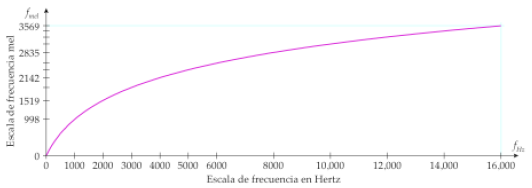
\includegraphics[width=0.65\textwidth]{Imagenes/Cap2/image041}
\end{center}
\begin{center}
\vskip -0.5cm
\caption{\small{Gráfica del arqueado de la frecuencia con la escala Mel.}}
\label{fig:figura2.40}
{\small{Fuente: \cite{eyra}}}
\end{center}
\end{figure}

\newpage
\item[•]Definición de las bandas criticas triangulares con la escala Mel
\par
El diseño de los filtros para las bandas críticas primero se realiza en la escala Mel. Los filtros utilizados en este método presentan una forma triangular, que es simétrica con respecto a su frecuencia central y tienen el mismo ancho de banda en la escala Mel.
\vskip 0.5cm
Aunque a estas ventanas triangulares se les suele llamar filtros, estas simplemente se usan para promediar el espectro de potencia con respecto a la frecuencia central de cada una de las bandas críticas. La función que las define está dada por la siguiente ecuación y su representación gráfica se muestra en la Figura \ref{fig:figura2.41}.
\begin{equation}
\label{eq:ecuacion49}
H_{bc}(f)= \left\{ \begin{array}{lcl}
0 & \mbox{ para } & f \leq f_{l} \\
& & \\
\frac{1}{(f_{c} - f_{l})}(f - f_{l}) & \mbox{ para } & f_{l} < f < f_{c} \\
& & \\
1 & \mbox{ para } & f = f_{c} \\
& & \\
\frac{- 1}{(f_{h} - f_{c})}(f - f_{h}) & \mbox{ para } & f_{c} < f < f_{h} \\
& & \\
0 & \mbox{ para } & f \geq f_{h} \\
\end{array}
\right.
\end{equation}

\begin{figure}[H]
\begin{center}
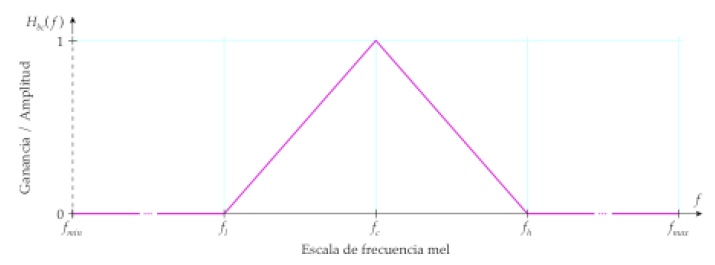
\includegraphics[width=0.5\textwidth]{Imagenes/Cap2/image042}
\end{center}
\begin{center}
\vskip -0.5cm
\caption{\small{Curva para las bandas críticas triangulares.}}
\label{fig:figura2.41}
{\small{Fuente: \cite{eyra}}}
\end{center}
\end{figure}

En la Ecuación \eqref{eq:ecuacion49} se puede apreciar que los primeros términos (cocientes) son las pendientes de las rectas que forman la ventana triangular, y los otros términos del producto contienen a la variable independiente con su respectiva abscisa al origen. Ahora bien, la transformación no lineal de la frecuencia en Hertz a la escala de frecuencia Mel, se acostumbra realizar mediante la función de aproximación Ecuación \eqref{eq:ecuacion48}.
\vskip 0.5cm
El rango de frecuencias de interés abarca desde los 0 Hz hasta la frecuencia de Nyquist, sin embargo, se puede determinar un límite inferior de frecuencia $f_{min}$, y un límite superior de frecuencia $f_{max}$. Para la señal de voz, se recomienda que $f_{min} > 100 Hz$ y que el límite superior de frecuencia sea menor a la frecuencia de Nyquist, aunque para una frecuencia mayor de 6800 Hz ya no hay mucha información en la señal de voz. Además, si se fija el límite inferior de frecuencia arriba de 50 o 60 Hz, se puede evitar el ruido procedente de la red de suministro o distribución de AC. Ahora bien, puesto que estos límites están definidos en Hertz, hace falta transformarlos a la escala Mel.
\begin{equation}
\label{eq:ecuacion50}
\left ( f_{min} \right )_{mel} = 1125\mathbf{Ln}\left ( 1 + \frac{f_{min}}{700} \right )
\qquad
\left ( f_{max} \right )_{mel} = 1125\mathbf{Ln}\left ( 1 + \frac{f_{max}}{700} \right )
\end{equation}
Las frecuencias centrales deben estar equiespaciadas en la escala Mel, entonces se puede calcular la separación en frecuencia entre éstas $SF$, mediante la siguiente fórmula:
\begin{equation}
\label{eq:ecuacion51}
SF = \frac{\left ( f_{max} \right )_{mel} - \left ( f_{min} \right )_{mel}}{BC + 1}
\end{equation}
\newpage
Las frecuencias centrales están separadas por múltiplos enteros de este parámetro más el valor del límite inferior de frecuencia:
\begin{equation}
\label{eq:ecuacion52}
f_{c}(bc)_{mel} = bc \cdot SF + \left ( f_{min} \right )_{mel}
\qquad
bc = 1,2,3,...,BC
\end{equation}
En donde $bc$ denota el número correspondiente de la banda crítica. Ahora sólo hace falta transformar las frecuencias centrales de la escala Mel a la escala en Hertz mediante la siguiente fórmula, que es la función inversa de la Ecuación \eqref{eq:ecuacion48}
\begin{equation}
\label{eq:ecuacion53}
f_{Hz}(f_{mel}) = 700\left [ e^{\left ( \frac{f_{mel}}{1125} \right )} - 1 \right]
\end{equation}
Con estos valores de las frecuencias centrales en Hertz, ya se pueden determinar las frecuencias inferior y superior para cada una de las bandas críticas. La frecuencia inferior para una banda crítica $bc$ es igual a la frecuencia central de la banda crítica anterior:
\begin{equation}
\label{eq:ecuacion54}
f_{l}(bc) = f_{c}(bc - 1)
\end{equation}
La frecuencia superior para una banda crítica es igual a la frecuencia central de la banda crtica posterior:
\begin{equation}
\label{eq:ecuacion55}
f_{h}(bc) = f_{c}(bc + 1)
\end{equation}
La frecuencia inferior de la primera banda crítica es igual al límite inferior de frecuencia:
\begin{equation}
\label{eq:ecuacion56}
f_{l}(1) = f_{min}
\end{equation}
De manera similar, la frecuencia superior de la última banda crítica es igual al límite superior de frecuencia.
\begin{equation}
\label{eq:ecuacion57}
f_{h}(BC) = f_{max}
\end{equation}
La Tabla \ref{table:tabla2.4} muestra los valores para las frecuencias inferior, central y superior para un banco de $BC =17$ filtros, tanto en la escala Mel como en la escala en Hertz. El límite inferior de frecuencia es $f_{min} = 0$ Hz y el límite superior de frecuencia es $f_{max} = 4000$ Hz.

\begin{center}
\begin{table}[h]
\centering
\caption{\small{Valores de las frecuencias para las bandas críticas triangulares.}}
\label{table:tabla2.4}
\vskip 0.2cm
\scalebox{0.75}{
\begin{tabular}{|c|c|c|c|c|c|c|c|}
\hline
{\small $\mathbf{bc}$} & {\small $\mathbf{fl}$} & {\small $\mathbf{fc}$} & {\small $\mathbf{fh}$} & {\small $\mathbf{fl}$} & {\small $\mathbf{fc}$} & {\small $\mathbf{fh}$}  \\ 
\hline 
{\small \textbf{[banda c.]}} & {\small \textbf{[mel]}} & {\small \textbf{[mel]}} & {\small \textbf{[mel]}} & {\small \textbf{[Hz]}} & {\small \textbf{[Hz]}} & {\small \textbf{[Hz]}}  \\ 
\hline 
{\small 1} & {\small 0.000} & {\small 119.015} & {\small 238.030} & {\small 0.00} & {\small 78.11} & {\small 164.94}  \\ 
\hline 
{\small 2} & {\small 119.015} & {\small 238.030} & {\small 357.045} & {\small 78.11} & {\small 164.94} & {\small 261.46}  \\ 
\hline 
{\small 3} & {\small 238.030} & {\small 357.045} & {\small 476.059} & {\small 164.94} & {\small 261.46} & {\small 368.75}  \\ 
\hline 
{\small 4} & {\small 357.045} & {\small 476.059} & {\small 595.074} & {\small 261.46} & {\small 368.75} & {\small 488.01}  \\ 
\hline 
{\small 5} & {\small 476.059} & {\small 595.074} & {\small 714.089} & {\small 368.75} & {\small 488.01} & {\small 620.58}  \\ 
\hline 
{\small 6} & {\small 595.074} & {\small 714.089} & {\small 833.104} & {\small 488.01} & {\small 620.58} & {\small 767.94}  \\ 
\hline 
{\small 7} & {\small 714.089} & {\small 833.104} & {\small 952.119} & {\small 620.58} & {\small 767.94} & {\small 931.75}  \\ 
\hline 
{\small 8} & {\small 833.104} & {\small 952.119} & {\small 1071.134} & {\small 767.94} & {\small 931.75} & {\small 1113.84}  \\ 
\hline 
{\small 9} & {\small 952.119} & {\small 1071.134} & {\small 1190.148} & {\small 931.75} & {\small 1113.84} & {\small 1316.24}  \\ 
\hline 
{\small 10} & {\small 1071.134} & {\small 1190.148} & {\small 1309.163} & {\small 1113.84} & {\small 1316.24} & {\small 1541.23}  \\ 
\hline 
{\small 11} & {\small 1190.148} & {\small 1309.163} & {\small 1428.178} & {\small 1316.24} & {\small 1541.23} & {\small 1791.33}  \\ 
\hline 
{\small 12} & {\small 1309.163} & {\small 1428.178} & {\small 1547.193} & {\small 1541.23} & {\small 1791.33} & {\small 2069.34}  \\ 
\hline 
{\small 13} & {\small 1428.178} & {\small 1547.193} & {\small 1666.208} & {\small 1791.33} & {\small 2069.34} & {\small 2378.37}  \\ 
\hline 
{\small 14} & {\small 1547.193} & {\small 1666.208} & {\small 1785.223} & {\small 2069.34} & {\small 2378.37} & {\small 2721.88}  \\ 
\hline 
{\small 15} & {\small 1666.208} & {\small 1785.223} & {\small 1904.237} & {\small 2378.37} & {\small 2721.88} & {\small 3103.72}  \\ 
\hline 
{\small 16} & {\small 1785.223} & {\small 1904.237} & {\small 2023.252} & {\small 2721.88} & {\small 3103.72} & {\small 3528.18}  \\ 
\hline 
{\small 17} & {\small 1904.237} & {\small 2023.252} & {\small 2142.267} & {\small 3103.72} & {\small 3528.18} & {\small 4000.00}  \\ 
\hline 
\end{tabular} 
}
\begin{center}
\vskip 0.2cm
{\small{Fuente: \cite{eyra}}}
\end{center}
\end{table}
\end{center}

En la Figura \ref{fig:figura2.42} se muestra la representación gráfica, en la escala Mel, del banco de filtros triangulares mostrado en la Tabla \ref{table:tabla2.4}. Las bandas críticas están equiespaciadas y todas las bandas críticas tienen el mismo ancho de banda.
\begin{figure}[H]
\begin{center}
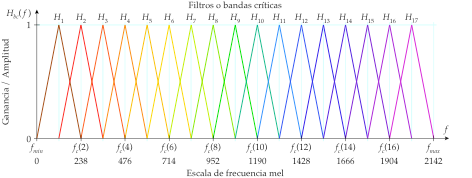
\includegraphics[width=0.6\textwidth]{Imagenes/Cap2/image043}
\end{center}
\begin{center}
\vskip -0.5cm
\caption{\small{Banco de filtros o ventanas triangulares equiespaciados en la escala Mel.}}
\label{fig:figura2.42}
{\small{Fuente: \cite{eyra}}}
\end{center}
\end{figure}
\vskip -0.5cm
La Figura \ref{fig:figura2.43} muestra el mismo banco de filtros, pero ahora en la escala en Hertz. Puede apreciarse como la distribución de las bandas críticas ahora sigue una distribución logarítmica y también como se incrementa el ancho de banda al aumentar la frecuencia.
\begin{figure}[H]
\begin{center}
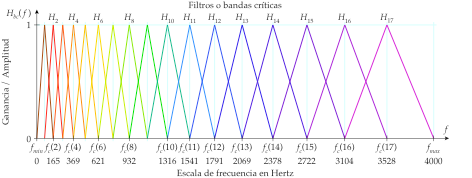
\includegraphics[width=0.6\textwidth]{Imagenes/Cap2/image044}
\end{center}
\begin{center}
\vskip -0.5cm
\caption{\small{Banco de filtros o ventanas triangulares en Hertz con distribución logarítmica.}}
\label{fig:figura2.43}
{\small{Fuente: \cite{eyra}}}
\end{center}
\end{figure}
\vskip -0.5cm
Finalmente, sólo hace falta hacer un muestreo de las bandas críticas de acuerdo al número de puntos del espectro de potencia $N_{p}.$ Ahora bien, como las bandas críticas contienen unos cuantos valores diferentes de cero, no hace falta calcular todos los valores correspondientes a cada uno de los puntos del espectro de potencia, basta con las muestras comprendidas entre la frecuencia inferior y la superior para cada banda crítica.
\vskip 0.5cm
A cada muestra del espectro de potencia $P(k)$ le corresponde un valor de frecuencia en Hertz, el cual es un múltiplo de la resolución en frecuencia del espectro:
\begin{equation}
\label{eq:ecuacion58}
f = k \cdot \Delta f
\qquad
k = 0,1,2,3,...,N_{p}
\end{equation}
La resolución en frecuencia del espectro $\Delta f$, se puede calcular mediante el cociente de la frecuencia de muestreo $f_{s}$, entre el número de puntos para la transformada rápida de Fourier $N_{fft}$:
\begin{equation}
\label{eq:ecuacion59}
\Delta f = \frac{f_{s}}{N_{fft}}
\end{equation}
Si se invierte este cociente, el nuevo factor es la resolución por muestra del espectro $\Delta k$:
\begin{equation}
\label{eq:ecuacion60}
\Delta k = \frac{N_{fft}}{f_{s}}
\end{equation}
El cual se puede utilizar para determinar que índice o muestra corresponde a determinada frecuencia, al multiplicar esa frecuencia por este factor de equivalencia:
\begin{equation}
\label{eq:ecuacion61}
k = \left ( f \cdot \Delta k  \right )_{\mathbf{int}}
\end{equation}
Puesto que los índices de las muestras deben ser números enteros, se tiene que redondear el resultado a un número entero. El índice para la frecuencia inferior $k_{l}$ se puede redondear hacia arriba, pero el índice para la frecuencia superior $k_{h}$ se puede redondear hacia abajo. También, si es necesario, hay que tomar en cuenta que la primera muestra del espectro de potencia representa a la frecuencia cero.
\vskip 0.5cm
Con los índices correspondientes a las frecuencias inferior $k_{l}$ y superior $k_{h}$, ya se pueden calcular los $N_{bc}$ valores diferentes de cero para cada una de las bandas críticas.
\begin{equation}
\label{eq:ecuacion62}
N_{bc} = k_{h}(bc) - k_{l}(bc) + 1
\end{equation}
Para esto, primero se obtiene el valor correspondiente en frecuencia para la muestra $k$, comprendida dentro del intervalo $k_{l}(bc) \leq k \leq k_{h}(bc)$ de una banda crítica $bc$. Entonces, el valor correspondiente a la muestra $k$ para el filtro o la banda crítica $H_{bc}$ se determina mediante la Ecuación \eqref{eq:ecuacion58}, según sea el caso.
\vskip 0.5cm
En la Tabla \ref{table:tabla2.5} se muestran los índices correspondientes a las frecuencias inferior y superior para las $BC =17$ bandas críticas de la Tabla \ref{table:tabla2.4} . El número de puntos para la transformada rápida de Fourier es de $N_{fft} = 256$ puntos y la frecuencia de muestreo es de $f_{s} = 8000$ Hz. Por lo tanto, la resolución en frecuencia es de $\Delta f = 31.25$ $Hz/muestra$, pero la resolución por muestra es de $\Delta k =0.032$ $muestras/Hz$.

\newpage
\begin{center}
\begin{table}[h]
\centering
\caption{\small{Correspondencia entre índices y frecuencias para las bandas críticas Mel.}}
\label{table:tabla2.5}
\vskip 0.2cm
\scalebox{0.75}{
\begin{tabular}{|c|c|c|c|c|c|c|c|c|}
\hline
{\small $\mathbf{bc}$} & {\small $\mathbf{fl}$} & {\small $\mathbf{kl}$} & {\small $\mathbf{(kl) int}$} & {\small $\mathbf{fh}$} & {\small $\mathbf{kh}$} & {\small $\mathbf{(kh) int}$} & {\small $\mathbf{Nbc}$}  \\ 
\hline 
{\small \textbf{[banda c.]}} & {\small \textbf{[Hz]}} & {\small \textbf{[índice]}} & {\small \textbf{[índice]}} & {\small \textbf{[Hz]}} & {\small \textbf{[índice]}} & {\small \textbf{[índice]}} & {\small \textbf{[muestras]}}  \\ 
\hline 
{\small 1} & {\small 0.00} & {\small 0.00} & {\small 0} & {\small 164.94} & {\small 5.28} & {\small 5} & {\small 6}  \\ \hline 
{\small 2} & {\small 78.11} & {\small 2.50} & {\small 3} & {\small 261.46} & {\small 8.37} & {\small 8} & {\small 6}  \\ \hline 
{\small 3} & {\small 164.94} & {\small 5.28} & {\small 6} & {\small 368.75} & {\small 11.80} & {\small 11} & {\small 6}  \\ \hline 
{\small 4} & {\small 261.46} & {\small 8.37} & {\small 9} & {\small 488.01} & {\small 15.62} & {\small 15} & {\small 7} \\ \hline 
{\small 5} & {\small 368.75} & {\small 11.80} & {\small 12} & {\small 620.58} & {\small 19.86} & {\small 19} & {\small 8}  \\ \hline 
{\small 6} & {\small 488.01} & {\small 15.62} & {\small 16} & {\small 767.94} & {\small 24.57} & {\small 24} & {\small 9}  \\ \hline 
{\small 7} & {\small 620.58} & {\small 19.86} & {\small 20} & {\small 931.75} & {\small 29.82} & {\small 29} & {\small 10}  \\ \hline 
{\small 8} & {\small 767.94} & {\small 24.57} & {\small 25} & {\small 1113.84} & {\small 35.64} & {\small 35} & {\small 11}  \\ \hline 
{\small 9} & {\small 931.75} & {\small 29.82} & {\small 30} & {\small 1316.24} & {\small 42.12} & {\small 42} & {\small 13}  \\ \hline 
{\small 10} & {\small 1113.84} & {\small 35.64} & {\small 36} & {\small 1541.23} & {\small 49.32} & {\small 49} & {\small 14}  \\ \hline 
{\small 11} & {\small 1316.24} & {\small 42.12} & {\small 43} & {\small 1791.33} & {\small 57.32} & {\small 57} & {\small 15}  \\ \hline 
{\small 12} & {\small 1541.23} & {\small 49.32} & {\small 50} & {\small 2069.34} & {\small 66.22} & {\small 66} & {\small 17}  \\ \hline 
{\small 13} & {\small 1791.33} & {\small 57.32} & {\small 58} & {\small 2378.37} & {\small 76.11} & {\small 76} & {\small 19}  \\ \hline 
{\small 14} & {\small 2069.34} & {\small 66.22} & {\small 67} & {\small 2721.88} & {\small 87.10} & {\small 87} & {\small 21}  \\ \hline 
{\small 15} & {\small 2378.37} & {\small 76.11} & {\small 77} & {\small 3103.72} & {\small 99.32} & {\small 99} & {\small 23}  \\ \hline 
{\small 16} & {\small 2721.88} & {\small 87.10} & {\small 88} & {\small 3528.18} & {\small 112.90} & {\small 112} & {\small 25}  \\ \hline 
{\small 17} & {\small 3103.72} & {\small 99.32} & {\small 100} & {\small 4000.00} & {\small 128.00} & {\small 128} & {\small 29}  \\ 
\hline 
\end{tabular} 
}
\begin{center}
\vskip 0.2cm
{\small{Fuente: \cite{eyra}}}
\end{center}
\end{table}
\end{center}

La Tabla \ref{table:tabla2.6} muestra la correspondencia entre los índices y las frecuencias para los puntos que definen la octava banda crítica Mel $H_{8}$. Se muestran los índices $k$ para las muestras del espectro de potencia y sus valores correspondientes de frecuencia en Hertz. La resolución en frecuencia es $\Delta f = 31.25$ $Hz/muestra$. Para fines ilustrativos, se incluyen los valores exactos de los tres límites para los cinco casos de la Ecuación \eqref{eq:ecuacion49}.

\newpage
\begin{center}
\begin{table}[h]
\centering
\caption{\small{Correspondencia entre los valores para la octava banda crítica Mel.}}
\label{table:tabla2.6}
\vskip 0.2cm
\scalebox{0.75}{
\begin{tabular}{|c|c|c|c|c|}
\hline
{\small $\mathbf{bc}$} & {\small $\mathbf{f}$} & {\small $\mathbf{CASO}$} & {\small $\mathbf{H8(k)}$} \\ 
\hline 
{\small \textbf{[índice]}} & {\small \textbf{[Hz]}} & {\small } & {\small } \\ 
\hline 
{\small 24} & {\small 750.00} & {\small $1 : f \leq  fl$} & {\small 0} \\ \hline 
{\small \textbf{kl(8)}} & {\small \textbf{767.94}} & {\small $\mathbf{1 : f \leq  fl}$} & {\small \textbf{0}} \\ \hline 
{\small 25} & {\small 781.25} & {\small $2 : fl < f < fc$} & {\small 0.0812} \\ \hline 
{\small 26} & {\small 812.50} & {\small $2 : fl < f < fc$} & {\small 0.2720} \\ \hline 
{\small 27} & {\small 843.75} & {\small $2 : fl < f < fc$} & {\small 0.4628} \\ \hline 
{\small 28} & {\small 875.00} & {\small $2 : fl < f < fc$} & {\small 0.6536} \\ \hline 
{\small 29} & {\small 906.25} & {\small $2 : fl < f < fc$} & {\small 0.8443} \\ \hline 
{\small \textbf{kc(8)}} & {\small \textbf{931.75}} & {\small $\mathbf{3 : f = fc}$} & {\small \textbf{1}} \\ \hline 
{\small 30} & {\small 937.50} & {\small $4 : fc < f < fh$} & {\small 0.9684} \\ \hline 
{\small 31} & {\small 968.75} & {\small $4 : fc < f < fh$} & {\small 0.7968} \\ \hline 
{\small 32} & {\small 1,000.00} & {\small $4 : fc < f < fh$} & {\small 0.6252} \\ \hline 
{\small 33} & {\small 1,031.25} & {\small $4 : fc < f < fh$} & {\small 0.4536} \\ \hline 
{\small 34} & {\small 1,062.50} & {\small $4 : fc < f < fh$} & {\small 0.2819} \\ \hline 
{\small 35} & {\small 1,093.75} & {\small $4 : fc < f < fh$} & {\small 0.1103} \\ \hline 
{\small \textbf{kh(8)}} & {\small \textbf{1,113.84}} & {\small $\mathbf{5 : f \geq  fh}$} & {\small \textbf{0}} \\ \hline 
{\small 37} & {\small 1,156.25} & {\small $5 : f \geq  fh$} & {\small 0} \\
\hline 
\end{tabular} 
}
\begin{center}
\vskip 0.2cm
{\small{Fuente: \cite{eyra}}}
\end{center}
\end{table}
\end{center}

\item[•]Compresión
\par
En lugar de simplemente usar la magnitud del espectro remuestreado mediante la escala Mel para calcular los MFCC, algunos investigadores han sugerido que es más provechoso el emplear una función logaritmo para calcular la energía total de las bandas críticas alrededor de las frecuencias centrales:
\begin{equation}
\label{eq:ecuacion63}
P_{sc}(bc) = \mathbf{log}[P_{s}(bc)]
\qquad
bc = 1,2,3,...,BC
\end{equation}
El procesamiento de la magnitud y la obtención de su logaritmo también se realizan en el oído humano. Es más, el empleo de la magnitud descarta la información innecesaria que proporciona la fase mientras que el logaritmo efectúa una compresión, dando como resultado que la extracción de características sea menos sensible a las variaciones de la amplitud producidas por las resonancias espectrales.

\item[•]Transformada inversa de Fourier
\par
El último paso en el cálculo de los MFCC consiste en realizar la transformada discreta inversa de Fourier del espectro muestreado y comprimido $P_{sc}$. En este paso es donde se obtienen los MFCC, además esta etapa del procedimiento tiene grandes ventajas, puesto que los valores del espectro son números reales y presentan una simetría par con respecto a la frecuencia de Nyquist, entonces se puede reducir a una DCT (Transformada Coseno Discreta) en lugar de la IFFT (Transformada Discreta Inversa de Fourier):
\begin{equation}
\label{eq:ecuacion64}
c_{m} = \sum_{bc = 1}^{BC}P_{sc}(bc)\mathbf{cos}\left [ \frac{\pi }{BC}\left ( bc - \frac{1}{2} \right ) m \right ]
\qquad
m = 0,1,2,3,...,M
\end{equation}
La transformada coseno discreta tiene la propiedad de producir características que prácticamente no están correlacionadas entre sí. De tal manera que se pueden usar matrices diagonales de covarianza en lugar de las matrices ordinarias de covarianza, con lo que se reduce en gran manera el trabajo de cómputo y el número de parámetros a estimar. Además, la transformada coseno discreta proporciona un suavizado del espectro si solamente se conservan los primeros coeficientes.
\vskip 0.5cm
Por lo tanto, la solución final es el vector o el conjunto de coeficientes MFCC:
\begin{equation}
\label{eq:ecuacion65}
\begin{aligned}
& \mathbf{V}_{mfcc} = C_{m} \\
& \mathbf{V}_{mfcc} = [C_{1},C_{2},C_{3},...,C_{M}]
\end{aligned}
\qquad
m = 1,2,3,...,M
\end{equation}
El coeficiente inicial $c_{0}$ representa el logaritmo de la energía promedio en la trama y se descarta, pues ésta se puede calcular directamente a partir de la señal de voz.

\item[•]Coeficientes delta y doble deltas
\par
Los cambios temporales en el espectro, tienen una importancia significativa en la percepción humana, una manera de capturar estos cambios es utilizando los coeficientes delta cuya finalidad es medir el cambio de los coeficientes en el tiempo, \cite{xuedong}. Las características a usar en un reconocedor usando MFCC con $F_{s}$ de 16 KHz, es la siguiente:
\vskip 0.5cm
Por frame analizado (ventaneamiento) se tendrá un vector $X_{k}$ , donde:
\begin{equation}
\label{eq:ecuacion66}
X_{k} = 
\begin{pmatrix}
C_{k}\\ 
\Delta C_{k}\\ 
\Delta \Delta C_{k}
\end{pmatrix}
\end{equation}

\begin{enumerate}
\item[-]$C_k$ son los 13 coeficientes MFCC 
\item[-]13 coeficientes delta MFCC
\begin{equation}
\label{eq:ecuacion67}
\Delta C_{k} = C_{k + 2} - C_{k - 2}
\end{equation}
\item[-]13 coeficientes doble delta MFCC
\begin{equation}
\label{eq:ecuacion68}
\Delta \Delta C_{k} = \Delta C_{k + 1} - \Delta C_{k - 1}
\end{equation}
\end{enumerate}
\end{enumerate}
\end{enumerate}

\subsubsection{Reconocimiento}
Una vez terminada la fase de extracción de características, debemos empezar con la tarea del reconocimiento automático. Al igual que en la extracción de características, el proceso de reconocer una señal de voz por una persona también es motivo del estudio de múltiples algoritmos que realizan esta tarea, tales como el DTW (Alineamiento Temporal Dinámico), HMM (Modelos Ocultos de Markov), ANN (Redes Neuronales), etc. ver en \citep{luna}. 
\vskip 0.5cm
Este bloque dentro de los sistemas de reconocimiento de locutor, consiste en la comparación de parámetros característicos o patrones de voz. Como se explicó en el diagrama de bloques en la Figura \ref{fig:figura2.6}, es necesario hacer la comparación de patrones de referencia contra los patrones de prueba y en base a una lógica de decisión reconocer al locutor.
\vskip 0.5cm
Una característica fundamental de los sistemas de reconocimiento es la forma en que los vectores característicos son combinados y comparados con los patrones de referencia. Para poder realizar estas operaciones es necesario definir una medida de distancia o distorsión entre los vectores característicos. Si las características a medir tienen la misma longitud, pues es fácil realizar esta operación. Sin embargo, el problema se presenta si tenemos dos patrones que corresponden a la misma palabra, pero pronunciadas a diferentes velocidades, este análisis se hace inadecuado.
\vskip 0.5cm
Es por ello que en este capítulo estudiaremos la técnica de \textit{Alineación Dinámica en el Tiempo} o \textit{Alineamiento Temporal Dinámico} (DTW) para comparar estos patrones, la cual a su vez servirá para construir los patrones de referencia. También se estudian las medidas de distorsión o similitud que se emplean. Además, de la lógica de decisión para reconocer a un locutor.
\vskip 0.5cm
\begin{enumerate}
\item[a)]Alineamiento Temporal Dinámico
\par
Se sabe que una palabra es más compleja que un sonido fijo y sus características espectrales varían lentamente en el tiempo. Por lo tanto, si se analiza sobre períodos cortos, estas características se vuelven estacionarias. Como resultado del análisis, se obtienen patrones de voz para cada segmento analizado. Estos patrones, son parámetros que representan las características espectrales del tracto vocal durante ese segmento de voz. El problema de realizar una comparación punto a punto de estos patrones se asocia a las variaciones que existen al pronunciar varias veces una palabra, aún cuando la palabra ha sido pronunciada por el mismo locutor. 
\vskip 0.5cm
Tales variaciones se deben a la rapidez de pronunciación, a la duración de la palabra completa, a los diferentes acentos y estilos de pronunciación. Todas esto influye notablemente en el resultado de la comparación entre los patrones de voz. Por este motivo, se necesita llevar a cabo una alineación en el tiempo de las variaciones de pronunciación para que el resultado de la comparación de patrones tenga un significado útil al momento de tomar la decisión de reconocer a un locutor.
\vskip 0.5cm
Para entender lo anterior, primero explicaremos el concepto de alineación en el tiempo de una palabra de prueba contra una de referencia y posteriormente la comparación de patrones de voz. En la Figura \ref{fig:figura2.44} se muestra el problema de alineación en el tiempo.
\begin{figure}[H]
\begin{center}
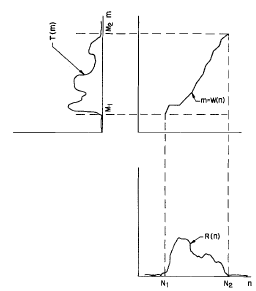
\includegraphics[width=0.45\textwidth]{Imagenes/Cap2/image045}
\end{center}
\begin{center}
\vskip -0.5cm
\caption{\small{Ilustración general de alineamiento en el tiempo de dos palabras.}}
\label{fig:figura2.44}
{\small{Fuente: \cite{rabiner}}}
\end{center}
\end{figure}

Se denota la palabra de referencia como $R(n)$ , $0 \leq n \leq N$ y la palabra de prueba como $T(m)$ , $0 \leq m \leq M$. El inicio y fin de $R(n)$ se denota como $N_{1}$ y $N_{2}$, y el inicio y fin de $T(m)$ como $M_{1}$ y $M_{2}$. El propósito del algoritmo de alineamiento en el tiempo es el de proveer un mapeo entre los índices temporales $n$ y $m$ para obtener una correspondencia en el tiempo entre las palabras de prueba y referencia. El mapeo $w$ o también llamado función de alineamiento (warping) entre $n$ y $m$ se denota como:
\begin{equation}
\label{eq:ecuacion69}
m = w(n)
\end{equation}
Donde $w$ debe satisfacer ciertas condiciones en el inicio y fin de las palabras. En el ejemplo de la Figura \ref{fig:figura2.44}, se asume que los puntos de inicio y fin de las palabras están alineados en el tiempo, es decir:
\begin{equation}
\label{eq:ecuacion70}
M_{1} = w(N_{1})
\end{equation}
\begin{equation}
\label{eq:ecuacion71}
M_{2} = w(N_{2})
\end{equation}
A estas condiciones de las Ecuaciones \eqref{eq:ecuacion70} y \eqref{eq:ecuacion71} se les llama conjunto restringido en los límites. Como se mencionó anteriormente, el análisis de una palabra se hace en períodos cortos, generalmente de 5 a 100 ms., por lo que para cada segmento de voz de la palabra analizada se obtienen parámetros característicos (en nuestro caso, los MFCC) con los cuales se construyen los patrones de voz para el locutor que pronunció la palabra.
\vskip 0.5cm
Ahora, si se consideran dos patrones de voz, $X$ y $Y$, representados por las secuencias ($x_{1}, x_{2},..., x_{n}$) y ($y_{1}, y_{2},..., y_{m}$) respectivamente, donde $x_{n}$ y $y_{m}$ son vectores que contienen los parámetros característicos de cada segmento de voz analizado, $N$ y $M$ son el número de segmentos en cada palabra y no necesariamente $N = M$. 
\vskip 0.5cm
El propósito del alineamiento en el tiempo de patrones de voz es el de obtener una función de alineamiento $w$ entre los índices temporales $n$ y $m$ con la cual se logre una correspondencia entre los patrones de voz de la palabra de prueba y los patrones de voz de la palabra de referencia. En la Figura \ref{fig:figura2.45}, se muestra un ejemplo de lo anterior donde se tienen los patrones de voz de la palabra de referencia en el eje de las ordenadas y los patrones de voz de la palabra de prueba en el eje de las abscisas. Se observa cómo la función de alineamiento proporciona una correspondencia entre los vectores $x_{n}$ y $y_{m}$ de los patrones de voz.
\begin{figure}[H]
\begin{center}
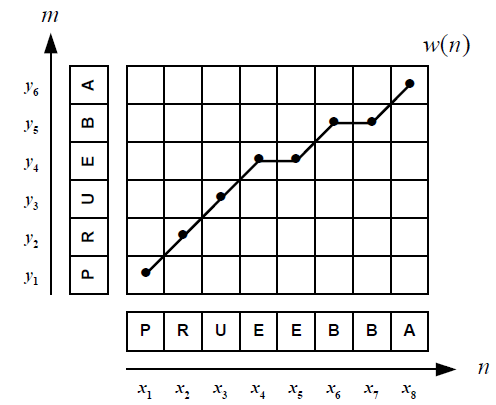
\includegraphics[width=0.4\textwidth]{Imagenes/Cap2/image046}
\end{center}
\begin{center}
\vskip -0.5cm
\caption{\small{Ejemplo de alineación de patrones de voz.}}
\label{fig:figura2.45}
{\small{Fuente: \cite{rabiner}}}
\end{center}
\end{figure}
La función de alineamiento debe cumplir con las Ecuaciones \eqref{eq:ecuacion70} y \eqref{eq:ecuacion71}, además de cumplir con ciertas suposiciones acerca de la forma de $w(n)$. Por ejemplo, si $w(n)$ es una función lineal, el alineamiento en el tiempo es simplemente una compresión o expansión de una escala en el tiempo. Esta función lineal asume que la variación en la pronunciación de una palabra es proporcional a la duración de la misma y es independiente del sonido hablado y por consiguiente no modela adecuadamente la forma en que se pronuncia una palabra, sobre todo no modela las variaciones de velocidad con que se pronuncian los sonidos vocales, por lo que es necesario emplear una función de alineamiento no lineal entre los patrones de voz.
\vskip 0.5cm
Un enfoque más sofisticado y poderoso para alinear en el tiempo, consiste en restringir a $w(n)$ para que satisfaga un conjunto de condiciones locales de continuidad,
\begin{equation}
\label{eq:ecuacion72}
w(n+1) - w(n) = 0,1,2(w(n) \neq w(n-1))
\end{equation}
\begin{equation}
\label{eq:ecuacion73}
w(n+1) - w(n) = 1,2(w(n) = w(n-1))
\end{equation}
estas ecuaciones hacen que $w(n)$ sea monotónicamente creciente con una pendiente máxima de 2 y una pendiente mínima de 0, excepto cuando la pendiente anterior fue 0, en tal caso la pendiente mínima será de 1. 
\vskip 0.5cm
Las condiciones de las Ecuaciones \eqref{eq:ecuacion70} y \eqref{eq:ecuacion71} junto con las condiciones de continuidad de las Ecuaciones \eqref{eq:ecuacion72} y \eqref{eq:ecuacion73} limitan a la función de alineamiento a seguir una trayectoria dentro del paralelogramo formado en el plano $(n, m)$ como se muestra en la Figura \ref{fig:figura2.46}. Los vértices, $A$ y $B$, del paralelogramo se obtiene de la intersección de las líneas,
\begin{equation}
\label{eq:ecuacion74}
\begin{aligned}
& m - 1 = 2(n - 1) \\
& m - M = (n - N)/2
\end{aligned}
\qquad
\text{Vértice A}
\end{equation}
y
\begin{equation}
\label{eq:ecuacion75}
\begin{aligned}
& m - 1 = (n - 1)/2 \\
& m - M = 2(n - N)
\end{aligned}
\qquad
\text{Vértice B}
\end{equation}

La función de alineamiento $w(n)$, está restringida a seguir una trayectoria dentro de la región sombreada de la Figura \ref{fig:figura2.46}.
\begin{figure}[H]
\begin{center}
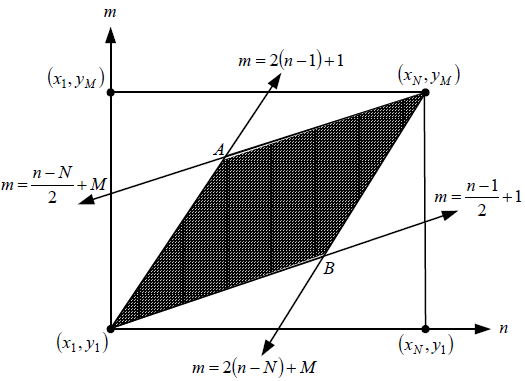
\includegraphics[width=0.45\textwidth]{Imagenes/Cap2/image047}
\end{center}
\begin{center}
\vskip -0.5cm
\caption{\small{Región de posibles trayectorias de la función de alineamiento.}}
\label{fig:figura2.46}
{\small{Fuente: \cite{rabiner}}}
\end{center}
\end{figure}
Para obtener la trayectoria de la función de alineamiento es necesario considerar una medida de similitud o distancia entre $X$ y $Y$, la cual se define considerando una distancia local $d(x_{n},y_{m})$. Esta distancia local se calcula para todos los vectores en el eje $n$ contra todos los vectores en el eje $m$ como se muestra en la Figura \ref{fig:figura2.47}. Por simplicidad esta distancia local será denotada como $d(n, m)$, donde $n = 1,2,...,N$, $m = 1,2,...,M$ y generalmente $N \neq M$. Entre más pequeño sea el valor de $d$, mayor es la similitud entre $x_{n}$ y $y_{m}$.
\begin{figure}[H]
\begin{center}
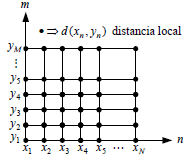
\includegraphics[width=0.3\textwidth]{Imagenes/Cap2/image048}
\end{center}
\begin{center}
\vskip -0.5cm
\caption{\small{Distancias locales generadas por los patrones de voz.}}
\label{fig:figura2.47}
{\small{Fuente: \cite{rabiner}}}
\end{center}
\end{figure}
\vskip -0.5cm
Dada la función de distancia local $d$, la trayectoria óptima de la función de alineamiento $w(n)$ acotada por el paralelogramo de la Figura \ref{fig:figura2.46}, debe de ser tal que la distancia acumulada total $D_{T}$ desde el punto $(x_{1}, y_{1})$ al punto $(x_{N}, y_{M})$ siguiendo a $w(n)$ sea mínima, es decir: 
\begin{equation}
\label{eq:ecuacion76}
D_{T} = \underset{\{w(n)\}}{min} \sum_{n=1}^{N}d(n,w(n))
\end{equation}
Donde $d(n,w(n))$ es la distancia local entre el segmento $n$ del patrón de referencia y el segmento $w(n)$ del patrón de prueba.
\vskip 0.5cm
Hasta este punto se ha mencionado la trayectoria óptima de la función de alineamiento, sin embargo, no se ha establecido un método para obtenerla. La técnica para determinarla es mediante el método de programación dinámica. Usando esta técnica, la distancia mínima acumulada a cualquier punto en el plano $(n,m)$ puede ser determinada en forma recursiva:
\begin{equation}
\label{eq:ecuacion77}
D_{A}(n,m) = d(n,m) + \underset{q \leq m}{min} D_{A}(n-1,q)
\qquad
\begin{aligned}
& n = 1,2,...,N \\
& m = 1,2,...,M
\end{aligned}
\end{equation}
Donde $D_{A}(n-1, q)$ es la distancia mínima acumulada al punto $(n-1, q)$, y $q$ puede tomar valores de $q = m, m - 1, m - 2$. Dadas las restricciones de continuidad de las Ecuaciones \eqref{eq:ecuacion72} y \eqref{eq:ecuacion73} y la Ecuación \eqref{eq:ecuacion77} puede ser escrita de la siguiente forma:
\begin{equation}
\label{eq:ecuacion78}
\begin{aligned}
D_{A}(n,m) = d(n,m) + min[D_{A}(n-1,m)g(n-1,m) , \\
D_{A}(n-1,m-1),D_{A}(n-1,m-2)]
\end{aligned}
\end{equation}
Donde:
\vskip 0.2cm
\begin{center}
$
g(n,m) = \left\{ \begin{array}{lcl}
1 & w(n) \neq w(n-1) \\
& \\
\infty & w(n) = w(n-1) \\
\end{array}
\right.
$
\end{center}
\vskip 0.5cm
En la Figura \ref{fig:figura2.48}, se muestra un ejemplo gráfico de las restricciones de continuidad, además, se muestra una restricción no lineal ya que si la mejor trayectoria al punto $(n - 1, m)$ viene del punto $(n - 2, m)$, entonces ninguna trayectoria puede salir del punto $(n - 1, m)$, a estas restricciones se les conoce como restricciones locales del tipo Itakura.
\begin{figure}[H]
\begin{center}
\includegraphics[width=0.35\textwidth]{Imagenes/Cap2/image049}
\end{center}
\begin{center}
\vskip -0.5cm
\caption{\small{Conjunto de posibles trayectorias hacia el punto (n, m).}}
\label{fig:figura2.48}
{\small{Fuente: \cite{rabiner}}}
\end{center}
\end{figure}

La función de alineamiento se obtiene a partir de la Ecuación \eqref{eq:ecuacion77}. Esta función contiene los índices $m$ donde $D_{A}(n - 1, q)$ es mínima para $q = m, m-1, m-2$ y $n = 2,3,...,N$, en otras palabras, la función de alineamiento contiene los índices para los cuales existe una correspondencia entre el índice $n$ del patrón de referencia y el índice $m$ del patrón de prueba.
\vskip 0.5cm
La iteración de la ecuación se realiza para todos los índices $m$ válidos, es decir, todos los índices $m$ dentro del paralelogramo de la Figura \ref{fig:figura2.46}, y para cada valor de $n$, desde $n = 1$ hasta $n = N$. La solución final o distancia total está dada como:
\begin{equation}
\label{eq:ecuacion79}
D_{T} = D_{A}(N,M)
\end{equation}
Las Ecuaciones \eqref{eq:ecuacion78} y \eqref{eq:ecuacion79} definen la técnica de programación dinámica para el alineamiento en el tiempo de patrones de voz. Al aplicarla a dos patrones de voz, se obtiene la medida de distancia total y la función de alineamiento. La función de alineamiento se usa en la etapa de entrenamiento, mientras que la distancia total entre los patrones de voz se emplea en la etapa de prueba.
\vskip 0.5cm
A este método de alineación en el tiempo se le conoce como inicio y fin con restricción, rango de la pendiente 2 a 1 (Constrained Endpoints 2 to 1 slope range, CE2-1) donde se asume que existe un alineamiento perfecto entre los puntos de inicio y fin de los patrones de voz de prueba y referencia. En la Figura \ref{fig:figura2.49}, se ilustra este método.
\begin{figure}[H]
\begin{center}
\includegraphics[width=0.3\textwidth]{Imagenes/Cap2/image050}
\end{center}
\begin{center}
\vskip -0.5cm
\caption{\small{Técnica de alineación dinámica en el tiempo CE2-1.}}
\label{fig:figura2.49}
{\small{Fuente: \cite{rabiner}}}
\end{center}
\end{figure}
Existen dos variantes del método explicado anteriormente. La primera variante se le conoce como inicio y fin sin restricción, rango de la pendiente 2 a 1 (Unconstrained Endpoints 2 to 1 slope range, UE2-1), ver la Figura \ref{fig:figura2.50}, se utiliza cuando se tiene cierto grado de incertidumbre en la detección del inicio y fin de la palabra. 
\vskip 0.2cm
\begin{figure}[H]
\begin{center}
\includegraphics[width=0.35\textwidth]{Imagenes/Cap2/image051}
\end{center}
\begin{center}
\vskip -0.5cm
\caption{\small{Técnica de alineación dinámica en el tiempo UE2-1.}}
\label{fig:figura2.50}
{\small{Fuente: \cite{rabiner}}}
\end{center}
\end{figure}
La segunda variante se le conoce como inicio y fin sin restricción, mínimos locales (Unconstrained Endpoints Local Mínimum, UELM), ver la Figura \ref{fig:figura2.51}. En este método, $w(n)$ se restringe a seguir la trayectoria local óptima dentro de un rango especificado.  El propósito de esta restricción adicional es el de reducir los cálculos ya que este algoritmo sigue la trayectoria local óptima para estimar la trayectoria global óptima.
\begin{figure}[H]
\begin{center}
\includegraphics[width=0.3\textwidth]{Imagenes/Cap2/image052}
\end{center}
\begin{center}
\vskip -0.5cm
\caption{\small{Técnica de alineación dinámica en el tiempo UELM.}}
\label{fig:figura2.51}
{\small{Fuente: \cite{rabiner}}}
\end{center}
\end{figure}

En \cite{rabiner2} se muestran comparaciones de estas tres variantes aplicadas en el reconocimiento de palabras aisladas y se concluye que:
\begin{enumerate}
\item[-]La variante CE2-1 genera distancias totales más grandes que la variante UE2-1.
\item[-]El algoritmo UE2-1 sirve para reducir la distancia total y para mejorar el desempeño del método.
\item[-]El algoritmo UELM se usa para aplicaciones en las cuales solamente se conoce el inicio de la palabra, por ejemplo, reconocimiento utilizando palabras concatenadas.
\end{enumerate}

Según \cite{rabiner3} se generan pequeñas pero consistentes mejoras en la exactitud de reconocimiento cuando el patrón de prueba está sobre la abscisa.

\vskip 0.5cm
En \citep{furui} se muestra que se produce menor tasa de error en la verificación de locutor cuando la palabra de menor duración se utiliza sobre la abscisa, independientemente que esta sea una palabra de prueba o de referencia.

\vskip 0.5cm
A partir de estos antecedentes, se ha optado para este trabajo de tesis el estudio de UE2-1 y UELM, a continuación explicaremos a detalle el algoritmo DTW.

\begin{enumerate}
\item[•]Restricciones de la función warping
\par
Tal como vimos anteriormente, la función warping, es una medida de la fluctuación en el eje del tiempo de los patrones del habla, la función $F = c(1), c(2),..., c(K)$, puede ser vista como una función de mapeo del patrón $A$ en el patrón $B$, quien debería conservar las estructuras lingüísticas esenciales en el patrón $A$ y viceversa, ver la Figura \ref{fig:figura2.52}.
\begin{figure}[H]
\begin{center}
\includegraphics[width=0.45\textwidth]{Imagenes/Cap2/image053}
\end{center}
\begin{center}
\vskip -0.5cm
\caption{\small{Función warping y ventana de ajuste.}}
\label{fig:figura2.52}
{\small{Fuente: \cite{sakoe}}}
\end{center}
\end{figure}

Las restricciones de la función warping \textit{F}, son las siguientes:
\begin{enumerate}
\item[-]Condición de monoticidad:
\begin{equation}
\label{eq:ecuacion80}
i(k - 1) \leq i(k)
\text{\quad y \quad}
j(k - 1) \leq j(k)
\end{equation}

\item[-]Condición de continuidad:
\begin{equation}
\label{eq:ecuacion81}
i(k) - i(k - 1) \leq 1
\text{\quad y \quad}
j(k) - j(k - 1) \leq 1
\end{equation}
como resultado de estas restricciones, la relación entre dos puntos consecutivos está dada:
\begin{equation}
\label{eq:ecuacion82}
c(k - 1) = \left\{ \begin{array}{lcl}
(i(k),j(k - 1)) \\
\\
(i(k - 1),j(k - 1)) \\
\\
(i(k - 1), j(k)) \\
\end{array}
\right.
\end{equation}

\item[-]Condición de frontera:
\begin{equation}
\label{eq:ecuacion83}
i(1) = 1, j(1) = 1
\text{\quad y \quad}
i(K) = I, j(K) = J
\end{equation}

\item[-]Condición de ventana de ajuste:
\begin{equation}
\label{eq:ecuacion84}
\left | i(k) - j(k)) \right | \leq  r
\end{equation}
Donde $r$ es un apropiado valor entero no negativo que indica el tamaño de la ventana de ajuste, esto se debe al hecho en que las fluctuaciones en el eje del tiempo, en algunos casos nunca causan excesiva diferencia.

\item[-]Condición de slope constraint:
\par
No se deben permitir gradientes ni muy pronunciadas, ni muy suaves para la función $F$, pues puede causar desviaciones no deseables en el eje del tiempo, para gradientes pronunciadas puede causar una correspondencia no real entre un patrón muy corto y otro muy largo.
\vskip 0.5cm
La condición de slope constraint es establecida como la primera derivada de la función warping en su forma discreta, así se obliga que los valores $c(k)$ se muevan en dirección hacia adelante en el eje $i$ o en el eje $j$, consecutivamente $m$ veces, entonces no se debe permitir que $c(k)$ vaya en la misma dirección a menos que haya pasado $n$ veces por la diagonal, la intensidad efectiva del slope constraint puede ser evaluada por la siguiente medida:
\begin{equation}
\label{eq:ecuacion85}
p = \frac{n}{m}
\end{equation}

\begin{figure}[H]
\begin{center}
\includegraphics[width=0.55\textwidth]{Imagenes/Cap2/image054}
\end{center}
\begin{center}
\vskip -0.5cm
\caption{\small{Slope constraint en función warping.}}
\label{fig:figura2.53}
{\small{Fuente: \cite{sakoe}}}
\end{center}
\end{figure}

Cuando $P = 0$, no existen restricciones en la función warping, cuando $P = \infty$ que significa $m = 0$ la función warping está restringida a la diagonal $i = j$, si el slope constraint es muy severo, entonces la normalización en el tiempo no podrá trabajar adecuadamente y si el slope constraint es muy relajado, entonces la discriminación entre patrones de diversas categorías es degradada, por ello es deseable un valor ni muy pequeño, ni muy grande de $p$.
\end{enumerate}

\item[•]Coeficientes de peso
\par
La expresión:
\begin{equation}
\label{eq:ecuacion86}
N = \sum_{k=1}^{K}w(k)
\end{equation}
que actúa como denominador del cálculo de la distancia normalizada:
\begin{equation}
\label{eq:ecuacion87}
D(A,B) = min\left [ \frac{\sum_{k=1}^{K}d(c(k))\cdot w(k)}{\sum_{k=1}^{K}w(k)} \right ]
\end{equation}
es independiente de la función warping $F$, luego la distancia normalizada se puede escribir como:
\begin{equation}
\label{eq:ecuacion88}
D(A,B) = \frac{1}{N} min\left [ \sum_{k=1}^{K}d(c(k))\cdot w(k) \right ]
\end{equation}
y puede ser efectivamente resuelto por la técnica de programación dinámica. Existen dos definiciones de coeficientes de pesos:

\begin{enumerate}
\item[-]Forma simétrica:
\begin{equation}
\label{eq:ecuacion89}
w(k) = (i(k) - i(k - 1)) + (j(k) - j(k - 1))
\end{equation}
entonces $N = I + J$, donde $I$ y $J$ son las longitudes de los parámetros de habla $A$ y $B$ respectivamente.
\item[-]Forma asimétrica:
\begin{equation}
\label{eq:ecuacion90}
w(k) = (i(k) - i(k-1))
\end{equation}
entonces $N = I$, o equivalentemente:
\begin{equation}
\label{eq:ecuacion91}
w(k) = j(k) - j(k - 1)
\end{equation}
entonces $N = J$.
\end{enumerate}

La forma simétrica significa que, si los ejes del tiempo $i$ y $j$ son continuos, entonces existirá un eje temporal: $l = i + j$ ; en la forma asimétrica se refiere a la integración a través del eje $i$ o $j$ según sea el caso. Según \citep{sakoe}, se espera que trabaje mejor la forma simétrica que la asimétrica, pues trata las partes del vector de características de igual manera, y la forma asimétrica hace alguna exclusión cuando la función warping está en dirección del eje $i$ o $j$ según sea el caso, pues $w(k)$ se reduce a cero: $c(k) = c(k-1)+(0,1)$, esto significa que algunos vectores pueden ser excluidos del análisis, pero por suerte la condición de slope constraint reduce esta situación, la diferencia de desempeño entre la forma simétrica y asimétrica puede ser gradualmente atenuada, del mismo modo que la condición de slope constraint es intensificada.

\begin{figure}[H]
\begin{center}
\includegraphics[width=0.5\textwidth]{Imagenes/Cap2/image055}
\end{center}
\begin{center}
\vskip -0.5cm
\caption{\small{Coeficientes de pesos para la forma simétrica y la forma asimétrica.}}
\label{fig:figura2.54}
{\small{Fuente: \cite{sakoe}}}
\end{center}
\end{figure}
\newpage
\item[•]Algoritmo PD-Matching
\par
El principio de PD (Programación Dinámica) puede ser aplicado a la definición de distancia normalizada en el tiempo, el algoritmo básico es descrito como sigue:
\vskip 0.5cm
Condición inicial:
\begin{equation}
\label{eq:ecuacion92}
g_{1}(c(1)) = d(c(1))w(1)
\end{equation}
Ecuaciones PD:
\begin{equation}
\label{eq:ecuacion93}
g_{k}(c(k)) = \underset{c(k-1)}{min}[g_{k-1}(c(k - 1)) + d(c(k)w(k))]
\end{equation}
Distancia normalizada en el tiempo:
\begin{equation}
\label{eq:ecuacion94}
D(A,B) = \frac{1}{N}g_{k}(c(k))
\end{equation}
Se asume que $c(0) = (0,0)$ y $w(1) = 2$ para la forma simétrica y $w(1) = 1$ para la forma asimétrica.
\vskip 0.5cm
Pueden derivarse varios algoritmos prácticos al aplicar la forma simétrica y la forma asimétrica según la condición de slope constraint que utilicen, algunos de ellos se detallan a continuación:
\vskip 0.5cm
Para el algoritmo de la forma simétrica la condición inicial de la Ecuación \eqref{eq:ecuacion92} quedaría así:
\begin{equation}
\label{eq:ecuacion95}
g(1,1) = 2d(1,1)
\end{equation}
Ecuación PD: para $p = 0$ en su forma simétrica
\begin{equation}
\label{eq:ecuacion96}
g(i,j) = min \left\{ \begin{array}{lcl}
g(i,j - 1) + d(i,j) \\
\\
g(i - 1 , j - 1) + 2d(i,j) \\
\\
g(i - 1,j) + d(i,j) \\
\end{array}
\right.
\end{equation}
Condición de restricción (ventana de ajuste):
\begin{equation}
\label{eq:ecuacion97}
j - r \leq i \leq j + r
\end{equation}
Distancia normalizada en el tiempo:
\begin{equation}
\label{eq:ecuacion98}
D(A,B) = \frac{1}{N}g(I,J)
\end{equation}
Las ecuaciones de PD $(g(i, j))$ se calculan en orden ascendente con respecto a las coordenadas $i$ y $j$, es decir empiezan de $(i, j)$ hasta $(I, J)$.

\begin{figure}[H]
\begin{center}
\includegraphics[width=0.5\textwidth]{Imagenes/Cap2/image056}
\end{center}
\begin{center}
\vskip -0.5cm
\caption{\small{Diagrama de flujo del algoritmo PD-Matching.}}
\label{fig:figura2.55}
{\small{Fuente: \cite{sakoe}}}
\end{center}
\end{figure}

Experimentos realizados en \citep{sakoe} muestran que el desempeño de la forma simétrica es superior al de la forma asimétrica, pero esta diferencia disminuye a medida que la condición de slope constraint es intensificada, se puede notar también que el desempeño de la forma simétrica no es afectado por un slope constraint superior a $P = 1$, por otro lado, la forma asimétrica es visiblemente mejorada por la condición de slope constraint. 
\vskip 0.5cm
Otro experimento hecho también en \citep{sakoe} evalúa el efecto de la condición de slope constraint en la forma simétrica del algoritmo PD-matching, y llega al resultado de que cuando $P = 1$ se obtiene el mejor desempeño, y en otro experimento evalúa este algoritmo con otros varios algoritmos PD propuestos por otros autores, y muestra la superioridad del algoritmo PD-matching con slope constraint $P = 1$. 
\vskip 0.5cm
En conclusión, se tiene que los mejores resultados se obtienen con la forma simétrica del algoritmo PD-matching y con una condición de slope constraint $P = 1$.

\begin{center}
\begin{table}[h!]
\centering
\vskip -0.2cm
\caption{\small{Algoritmos simétricos y asimétricos con condición de Slope Constraint P = 0, 1/2, 1, 2.}}
\label{table:tabla2}
\begin{tabular}{c}
\begin{minipage}{.9\textwidth}
\begin{center}
\includegraphics[width=0.85\textwidth]{Imagenes/Cap2/image057}
\end{center}
\end{minipage}
\end{tabular}
\begin{center}
\vskip 0.2cm
{\small{Fuente: \cite{sakoe}}}
\end{center}
\end{table}
\end{center}

\end{enumerate}

\item[b)]Distancias o medidas de distorsión
\par
Un componente clave en la mayoría de los algoritmos de comparación de patrones, es formular una medida de distorsión entre dos vectores característicos. Esta medida, puede ser manejada con rigor matemático si los patrones son visualizados en un espacio vectorial.
\vskip 0.5cm
Suponer que se tienen dos vectores característicos, $x$ e $y$, definidos en un espacio vectorial $X$. Se define una métrica o función de distancia, $d$, en el espacio vectorial $X$, como una función de valor real, sobre el producto cartesiano $X*X$, para que una función de distancia pueda tratarse con rigor matemático, debe satisfacer las siguientes condiciones:
\begin{enumerate}
\item[1.]$0 \leq  d(x, y) < \infty$, para $x, y$ $\epsilon$ $X$ y $d(x,y) = 0$ sí y solo sí $x = y$
\item[2.]$d(x, y) = d(y, x)$ para $x, y$ $\epsilon$ $X$
\item[3.]$d(x, y) \leq  d(x, z) + d(z, y)$ para $x, y, z$ $\epsilon$ $X$
\end{enumerate}
Además, una función de distancia se denomina invariante si:
\begin{enumerate}
\item[4.]$d(x + z, y + z) = d(x,y)$
\end{enumerate}

Las primeras tres propiedades comúnmente son conocidas como positividad, simetría y desigualdad del triángulo, respectivamente. Una métrica que contenga estas propiedades, permite un alto grado de manejo matemático. Sí una medida de distancia \textit{d}, satisface solo la propiedad de positividad, se le denomina medida de distorsión, particularmente cuando los vectores son representaciones del espectro de la señal.
\vskip 0.5cm
Para el procesamiento de voz es importante considerar que la elección, de la medida de distancia, es significativamente subjetiva. Una medida matemática de la distancia, para ser utilizada en el procesamiento de voz, debe tener una alta correlación entre su valor numérico y su distancia subjetiva aproximada, para evaluar una señal real de voz. 
\vskip 0.5cm
Para el reconocimiento de voz, la consistencia psicofísica (los diferentes matices que se le pueden imprimir a una misma palabra) que se desea medir con la distancia, obliga a que se encuentre una medida matemática ajustada por necesidad a las características lingüísticas conocidas. Estos requisitos tan subjetivos no pueden ser satisfechos con medidas de distancia que proporcionen manejo matemático, dado que existe una enorme dificultad al querer cumplir simultáneamente ambos objetivos (subjetividad y manejo matemático), algún compromiso es inevitable. Por consiguiente, y dado que se necesita manipular matemáticamente las propiedades de esa medida de distancia, se necesita probar que estas propiedades subjetivas son lo suficientemente buenas como para lograr el reconocimiento de voz. 
\vskip 0.5cm
Por otra parte, se hablará de \textit{medidas de distorsión} en vez de \textit{métricas} o \textit{distancias} debido a que se relajan las condiciones de simetría y desigualdad del triángulo. Por lo tanto, no se debe utilizar el término distancia en sentido estricto, acorde a la definición expuesta; por otro lado, en la costumbre de la literatura de voz el término distancia es análogo a las medidas de distorsión.
\vskip 0.5cm
Existen varios tipos de medidas de distorsión, cada una con sus características especiales, entre ellas tenemos: \textit{Distancia Euclidiana Cuadrática, Distorsión del Error Cuadrático Medio, Distorsión del Error Cuadrático Ponderado, Distancia de Itakura, Distancia de Mahalanosis}, etc., ver en \citep{navarrete}.
\vskip 0.5cm
Para este trabajo de tesis veremos solo la Distancia Euclidiana Cuadrática y la Distancia del Error Cuadrático Medio, debido a su sencillez y poca complejidad, además de complementarse muy bien con el algoritmo DTW.

\begin{enumerate}
\item[-]Distancia Euclidiana Cuadrática
\par
La medida más conveniente y ampliamente usada para calcular distancias, es el \textit{Error Cuadrático} o \textit{Distancia Euclidiana Cuadrática}, entre dos vectores, definida como:
\begin{equation}
\label{eq:ecuacion99}
d(X_{1},X_{2}) = \left \| X_{1} - X_{2} \right \|^{2} = \sum_{j=1}^{N}(X_{1j} - X_{2j})^2
\end{equation}

\item[-]Distorsión del Error Cuadrático Medio
\par
La distorsión del \textit{Error Cuadrático Medio} (MSE) es otra de las medidas más utilizadas, en la cual la distorsión está definida por cada dimensión y se define como:
\begin{equation}
\label{eq:ecuacion100}
d(X_{1},X_{2}) = \frac{1}{N}(X_{1} - X_{2})^{T}(X_{1} - X_{2}) = \frac{1}{N}\sum_{j=1}^{N}(X_{1j} - X_{2j})^2
\end{equation}
\end{enumerate}

\vskip 0.5cm
\item[c)]Construcción del patrón de referencia
\par
El sistema de identificación de locutor se divide en dos etapas, etapa de prueba y etapa de entrenamiento. En la etapa de prueba, basta con obtener la distancia total $D_{T}$ entre los patrones de voz. Con esta distancia total y una lógica de decisión se lleva a cabo la tarea de identificar a un locutor, esta lógica de decisión se verá más adelante. Sin embargo, para construir un patrón de referencia confiable para un locutor, en la etapa de entrenamiento, es necesario conocer la función de alineamiento, $w(n)$. Como se observa en la Figura \ref{fig:figura2.52}, la función de alineamiento provee una correspondencia entre los índices de los patrones de voz. Utilizando esta correspondencia entre los patrones de voz, se puede crear un patrón de referencia $z$, simplemente promediando los vectores de los patrones de voz siguiendo la función de alineamiento, es decir:
\begin{equation}
\label{eq:ecuacion101}
z_{n} = \frac{X_{n} + Y_{w(n)}}{2}
\qquad
n=1,2,...,N
\end{equation}
En \citep{furui}, el entrenamiento se hace de la siguiente manera: Primeramente, se tienen los patrones de voz para una palabra clave, pronunciada dos veces por el locutor. Se aplica la técnica de alineación dinámica en el tiempo y se obtiene la función de alineamiento para los dos patrones de voz.
\vskip 0.5cm
Se utiliza la Ecuación \eqref{eq:ecuacion101}, para crear el primer patrón de entrenamiento. Se repite este procedimiento para la misma palabra pronunciada por tercera ocasión, pero ahora comparada contra el primer patrón de entrenamiento. Se obtiene la función de alineamiento y utilizando de nuevo la Ecuación \eqref{eq:ecuacion101}, se genera el segundo patrón de entrenamiento. Este procedimiento se sigue hasta que se ha generado el quinto patrón de entrenamiento, el cual ya se considera como un patrón de referencia. Para obtener un patrón de referencia más confiable, se utiliza un mayor número de repeticiones de la palabra clave.

\item[d)]Toma de Decisión
\par
Después de realizar la comparación de patrones es necesario tener una lógica de decisión para identificar al locutor. Este es el último paso dentro de los sistemas de reconocimiento de locutor y consiste en escoger cuál patrón de referencia (locutores conocidos) mejor corresponde con el patrón de prueba (locutor desconocido). 
\vskip 0.5cm
La forma más simple de implementar lo anterior consiste en utilizar la regla del vecino más cercano, la cual opera de la siguiente manera: se tienen $V$ patrones de referencia, $R^{i}$, $i = 1,2,...,V$, donde cada patrón de referencia representa la identidad de un locutor, y para cada patrón de referencia se obtiene la distancia total $D^{i}_{T}$, $i = 1,2,...,V$, respecto al patrón de prueba utilizando el algoritmo DTW. El patrón de referencia con la distancia mínima respecto al patrón de prueba corresponderá a la identidad del locutor.
\vskip 0.5cm
Bueno, hasta aquí se ha considerado que el sistema es de conjunto cerrado, es decir, se tienen $N$ usuarios y $N$ decisiones del sistema. Sin embargo, esto da lugar a tres respuestas del sistema: que el sistema identifique a un usuario válido, que se equivoque en identificar a un usuario y que acepte a un intruso. Dado que se requiere que el sistema no acepte intrusos, se incluyen umbrales en el sistema con el fin de aumentar la seguridad del mismo. Con estos umbrales se pretende tener un sistema de $N$ usuarios y $N+1$ decisiones.
\vskip 0.5cm
Es por ello que se utilizaran umbrales individuales para poder incluir en el sistema de identificación de locutor la respuesta \textit{no identificado}. A cada locutor o patrón de referencia le corresponde un umbral. El cálculo de los umbrales se hace mediante un método explicado en \citep{varela}, donde se define una distancia \textit{intralocutor} y una distancia \textit{interlocutor}, el primero se obtiene al comparar mediante el algoritmo DTW el patrón de referencia de un locutor contra las palabras habladas por el mismo, y el segundo se obtiene al comparar el patrón de referencia de un locutor contra las palabras habladas por la base de datos de locutores sin incluir las palabras que pertenecen al locutor del cual se usa el patrón de referencia. 
\vskip 0.5cm
Se supone que tanto el conjunto de distancias intralocutor, como el de distancias interlocutor pueden ser aproximados por distribuciones de probabilidad normal como se muestra en la Figura \ref{fig:figura2.57}.

\begin{figure}[H]
\begin{center}
\includegraphics[width=0.5\textwidth]{Imagenes/Cap2/image058}
\end{center}
\begin{center}
\vskip -0.5cm
\caption{\small{Distribuciones de probabilidad de las distancias intralocutor e interlocutor.}}
\label{fig:figura2.57}
{\small{Fuente: \cite{varela}}}
\end{center}
\end{figure}

El umbral $U$ es el punto en donde el área bajo la curva de la distribución intralocutor desde $U$ a más infinito es igual al área bajo la curva de la distribución interlocutor desde menos infinito a $U$, es decir, el punto donde la probabilidad de que el sistema responda \textit{no identificado} es igual a la probabilidad de que exista una \textit{falsa identificación}. Las distribuciones de probabilidad normal de la Figura \ref{fig:figura2.57}. están dadas por la siguiente ecuación:
\begin{equation}
\label{eq:ecuacion102}
P(D) = \frac{1}{\sqrt{2 \pi \sigma }}e^{\frac{(D - \mu)^{2}}{2 \sigma^{2}}}
\end{equation}
Donde $\mu$ es la media y $\sigma$ es la desviación estándar. El umbral $U$ se calcula a partir de las siguientes ecuaciones:
\begin{equation}
\label{eq:ecuacion103}
U - \mu_{int ra} = n \sigma_{int ra}
\end{equation}
\begin{equation}
\label{eq:ecuacion104}
\mu_{int er} - U = n \sigma_{int er}
\end{equation}
despejando $n$ de las Ecuaciones \eqref{eq:ecuacion103} y \eqref{eq:ecuacion104} e igualando se obtiene el umbral $U$ de la siguiente forma:
\begin{equation}
\label{eq:ecuacion105}
U = \frac{\sigma_{int ra}\mu_{int er} + \sigma_{int er}\mu_{int ra}}{\sigma_{int ra} + \sigma_{int er}}
\end{equation}
Si es que se tienen 10 patrones de referencia (10 usuarios del sistema), es necesario calcular un umbral por cada patrón de referencia, es decir:
\begin{equation}
\label{eq:ecuacion106}
U_{i} = \frac{\sigma^{int ra}_{i} \mu^{int er}_{i} + \sigma^{int er}_{i} \mu^{int ra}_{i}}{\sigma^{int ra}_{i} + \sigma^{int er}_{i}}
\qquad
i = 1,2,...,9
\end{equation}
\end{enumerate}
\vskip 0.5cm
\section{Método de la investigación}
\subsection{Diseño de la investigación}
De acuerdo al fin que persigue, el presente trabajo es una investigación aplicada. Por otro lado, de acuerdo al diseño de contrastación de la hipótesis es una investigación experimental.

\subsection{Instrumentos}
\begin{enumerate}
\item[-]Un dispositivo móvil con Android 8.0, memoria RAM 3GB y CPU 4x1.4GHz.
\item[-]Un módem router pasarela con tecnología 802.11 b,g,n.
\item[-]Un computador con Windows 10, memoria RAM 8GB y CPU Intel Core i5 2x2.60GHz.
\item[-]Un Arduino Mega 2560 R3.
\item[-]Un módulo Ethernet Shield W5100 compatible con Arduino Mega.
\item[-]Un módulo relé 4 Songle 10A 250VAC.
\item[-]Un transformador DC 9-12V 1A.
\item[-]Un transformador DC 5V 500mA.
\item[-]Un transformador DC 12V 1A.
\item[-]Una cerradura eléctrica YALE.
\end{enumerate}

\subsection{Población y muestra}
Siendo una investigación experimental, la determinación de la muestra se basa en los antecedentes \cite{perez} y \cite{navarrete} debido a que estás investigaciones son de caso similar y en la experiencia del autor.
\vskip 0.5cm
Para esta tesis la población estará conformada por un conjunto de 800 audios dividido entre los comandos de voz \textit{Abrir} y los \textit{Nombres de los Usuarios} (Edwin, Carlos, Josué, Édison, Gerson, Nizama, Anthony, Jhordan, Renzo y Franchesco), los cuales serán las palabras claves de acceso para 10 miembros de la vivienda.
\vskip 0.5cm
La muestra está conformada por el conjunto de los 11 comandos de voz antes mencionados.
\newpage
\subsection{Variables de estudio}
\begin{enumerate}
\item[•]\textbf{Variable dependiente:} Control de acceso a una vivienda.
\item[•]\textbf{Variable independiente:} Sistema de seguridad por reconocimiento de voz.
\end{enumerate}

El factor de medida para el control de acceso a una vivienda mediante el reconocimiento de voz consiste en el tiempo de respuesta y la tasa de precisión en el reconocimiento que se obtengan de los resultados experimentales.

\subsection{Métodos y procedimientos para la recolección de datos}
Para recolectar los datos se harán grabaciones a 10 personas escogidas aleatoriamente, para esto se contará con el micrófono del dispositivo móvil y el del computador. El procedimiento a emplear será darle a cada persona la lista de los 2 comandos de voz (\textit{Abrir} y su \textit{Nombre}), las cuales, al ser leídas, serán grabadas. El nivel de ruido de la grabación deberá ser moderado.

\subsection{Método de estudio}
Para llegar a los objetivos propuestos, el desarrollo de la investigación comprendió las siguientes etapas:
\begin{enumerate}
\item[a)]Análisis del problema de los sistemas de control de acceso en la ciudad de Trujillo, en el Perú y el mundo, comprendiendo la situación actual y el levantamiento de los principales casos de éxito.
\item[b)]Formulación del problema principal de la investigación y justificación de la importancia de su solución.
\item[c)]Levantamiento de los diferentes temas necesarios para la elaboración de la investigación.
\item[d)]Diseño e implementación del software de reconocimiento de voz.
\item[e)]Diseño y construcción del hardware capaz de ser controlado a través del protocolo de red inalámbrica 802.11g.
\item[f)]Integración de las dos partes mencionadas anteriormente, así como la ejecución de pruebas para su correcto funcionamiento.
\item[g)]La implementación de todo el sistema en un ambiente real.
\item[h)]Realización del reporte de incidencias ocurridas mientras estaba en uso el sistema.
\end{enumerate}

\subsection{Análisis estadístico de los datos}
Para efectuar el análisis estadístico de los datos se hará la prueba de independencia Chi- Cuadrado de Pearson para dos variables nominales.
\vskip 0.5cm
El uso de esta prueba es que permite contrastar los resultados de una prueba o método propuesto, determinando si dos cualidades o variables referidas a individuos de una población están relacionadas. 

\subsection{Esquema general del proyecto}
En la Figura \ref{fig:figura2.58} se muestra el diagrama de bloques para el esquema general de este proyecto, primero la señal voz es capturada por el micrófono del dispositivo móvil, en el caso de que se habilite la opción de filtrado de ruido en el sistema, el micrófono del computador capturara la señal de ruido, luego el sistema se encargará de procesar y analizar la señal de voz (con la señal de ruido, si es que la hubiera) y dependiendo de la respuesta del reconocimiento de dicha señal este le enviará o no una señal al microcontrolador que controla el acceso, activando o no la cerradura eléctrica.
\vskip 0.5cm
\begin{figure}[H]
\begin{center}
\includegraphics[width=0.8\textwidth]{Imagenes/Cap2/image059}
\end{center}
\begin{center}
\vskip -0.5cm
\caption{\small{Diagrama de bloques general del proyecto.}}
\label{fig:figura2.58}
{\small{Fuente: Elaboración propia}}
\end{center}
\end{figure}                % Marco teórico
\chapter{Sistema de control de acceso por reconocimiento de voz}

Para el desarrollo del sistema se utilizará la metodología propuesta por \citep{tammy} , la cual toma mucha de las claves de las metodologías conocidas como RUP (Rational Unified Process), ADD (Attribute Driven Desing), OPP (Object Oriented Process) y el MDA (Model Driven Architecture), pero las simplifica. La Figura \ref{fig:figura3.1} muestra las diferentes fases de la metodología, la cual es definida por el autor como el \textit{Diseño del Sistema Empotrado y el Modelo del Ciclo de Vida del Desarrollo}.

\begin{figure}[H]
\begin{center}
\includegraphics[width=1.0\textwidth]{Imagenes/Cap3/image001}
\end{center}
\begin{center}
\vskip -0.5cm
\caption{\small{Diseño del sistema empotrado y el modelo del ciclo de vida del desarrollo.}}
\label{fig:figura3.1}
{\small{Fuente: \cite{tammy}}}
\end{center}
\end{figure}

Como se puede ver en la Figura \ref{fig:figura3.1}, en el diseño de un sistema empotrado, según la metodología de \cite{tammy}, se pueden distinguir 4 fases: 
\begin{enumerate}
\item[-]\textbf{Fase 1. Creación de la arquitectura}, el cual es el proceso de planear el diseño del sistema empotrado.
\item[-]\textbf{Fase 2. Implementación de la arquitectura}, el cual es el proceso de desarrollar el sistema empotrado. 
\item[-]\textbf{Fase 3. Testeo del sistema}, el cual es el proceso de testear el sistema empotrado para buscar problemas y luego solucionarlos. 
\item[-]\textbf{Fase 4. Mantenimiento del sistema}, el cual es el proceso de desplegar el sistema empotrado en el mercado, y proveerlo de soporte técnico para los usuarios del dispositivo por la duración del tiempo de vida del mismo.
\end{enumerate}

\section{Fase 1. Creación de la arquitectura}
Esta fase se divide en 3 etapas:
\begin{enumerate}
\item[-]Etapa 1: Tener una base técnica sólida.
\item[-]Etapa 2: Entender el ciclo de negocio de la arquitectura.
\item[-]Etapa 3: Definir los patrones arquitectónicos y modelos de referencia.
\end{enumerate}

\subsection{Etapa 1: Tener una base técnica sólida}
Esta etapa tiene como fundamento la base cognitiva de los autores de la presente tesis y ha sido descrita tanto en el título, introducción y marco teórico.

\subsection{Etapa 2: Entender el ciclo de negocio de la arquitectura}
En la Figura \ref{fig:figura3.2} vemos que el ciclo de negocio de la arquitectura de un sistema empotrado son los diferentes tipos de influencias los que generan los requerimientos del sistema, los requerimientos a su vez generan la arquitectura, luego esta produce el sistema y el sistema resultante a su vez provee los requerimientos y capacidades devuelta a la organización para futuros diseños.
\begin{figure}[H]
\begin{center}
\includegraphics[width=0.5\textwidth]{Imagenes/Cap3/image002}
\end{center}
\begin{center}
\vskip -0.5cm
\caption{\small{Ciclo de negocio de la arquitectura.}}
\label{fig:figura3.2}
{\small{Fuente: \cite{tammy}}}
\end{center}
\end{figure}

Una vez entendido el ciclo de negocio de la arquitectura, se debe plasmar la información obtenida de varias influencias, que en otras palabras son los requerimientos. La presente metodología propone hacerlo mediante la tabla general de características del ciclo de negocio de la arquitectura o el uso de prototipos. Se eligió representar los requerimientos mediante la tabla general de características del ciclo de negocio de la arquitectura, ver la Tabla \ref{table:tabla3.1}.

\begin{center}
\begin{table}[H]
\centering
\caption{\small{Características generales del ciclo de negocio de la arquitectura.}}
\label{table:tabla3.1}
\vskip 0.2cm
\begin{tabular}{|p{3cm}|p{4cm}|p{6cm}|p{3cm}|}
\hline
{\small Influencia} & {\small Característica} & {\small Descripción}  \\ 
\hline 
{\small \multirow{3}{4em}{Negocios}} & {\small Costo} & {\small El sistema de seguridad para el control de acceso por medio de la voz, debe tener un costo de desarrollo menor a los S/. 500.}  \\ 
\cline{2-3}
 & {\small Objetivo de Mercado} & {\small El sistema a diseñar es del tipo de módulo reconocedor de la voz y está dirigido al control de acceso, sin embargo, puede ser usado para el control de cualquier otro objeto.}  \\ 
\cline{2-3}
 & {\small Capacidad} & {\small El sistema debe poder reconocer la voz con una tasa de acierto del 95\%. El sistema debe poder controlar los accesos para nuevos de usuarios. El sistema debe poder dar información de todos los accesos que tuvo un usuario. El sistema debe poder permitir o denegar el acceso a un usuario. El sistema debe ser capaz de trabajar en ambientes con ruido no mayores a 80 dBC.
} \\
\hline 
{\small \multirow{4}{4em}{Técnicos}} & {\small Desempeño} & {\small El sistema debe ser capaz de reconocer una señal de voz en un tiempo menor o igual a 5 segundos. Sim embargo, la rapidez de respuesta del sistema dependerá de la cantidad de usuarios registrados en el sistema}  \\ 
\cline{2-3}
 & {\small Amistad con Usuario} & {\small La interfaz de usuario del sistema no será muy compleja, y solo mostrará lo necesario para su manipulación.}  \\ 
\cline{2-3}
 & {\small Modificabilidad} & {\small La modificación dependerá únicamente de los desarrolladores del software}  \\ 
\cline{2-3}
 & {\small Portabilidad} & {\small El sistema podrá ser usado por cualquier dispositivo móvil Android superior a 4.4
y menor a 9.0, por lo que será portable para la mayoría de los dispositivos existentes en el mercado aproximadamente el 95\%.}  \\ 
\hline 
\end{tabular} 
\begin{center}
\vskip 0.2cm
{\small{Fuente: Elaboración propia}}
\end{center}
\end{table}
\end{center}

\subsection{Etapa 3: Definir el patrón arquitectónico y modelo de referencia}
El patrón arquitectónico a usar será el patrón arquitectónico en capas y el modelo de referencia será el modelo de referencia de sistemas empotrados, definido en \citep{tammy}. El modelo de referencia para un sistema empotrado está construido en capas y no es más que una distribución topológica de los elementos del patrón arquitectónico en capas, se define que todo sistema empotrado está formado por tres capas: de hardware, de software de sistema y de aplicación.

\begin{enumerate}
\item[a)]Capa de hardware
\par
Esta capa estará formada principalmente por un microcontrolador Arduino, el cual alojará el controlador para la activación de la cerradura eléctrica por medio del módulo relé, además este se acoplará con el módulo Ethernet Shield, lo que permitirá conectarse a un router para poder establecer así la comunicación con el dispositivo móvil.

\item[b)]Capa de software de sistema
\par
Esta capa estará formada por el controlador para la activación de la cerradura eléctrica y por el servidor para poder establecer la comunicación con la aplicación de reconocimiento de voz alojado en el dispositivo móvil.

\item[c)]Capa de software de aplicación
\par
El sistema estará formado por hardware de propósito específico, diseñado solamente para la demostración de la aplicación de reconocimiento de voz, el cual estará compuesto por 3 módulos: preprocesamiento, entrenamiento y reconocimiento de la señal de voz.

\item[d)]Modelo de referencia
\par
El modelo de referencia servirá para aproximarse al posible hardware y software que deberá contener el sistema incorporando elementos relativos. La Figura \ref{fig:figura3.3} muestra el modelo de referencia del sistema de seguridad para el control de acceso por reconocimiento de voz.
\begin{figure}[H]
\captionsetup{justification=centering}
\begin{center}
\includegraphics[width=0.43\textwidth]{Imagenes/Cap3/image003}
\end{center}
\begin{center}
\vskip -0.5cm
\caption{\small{Modelo de referencia del sistema.}}
\label{fig:figura3.3}
{\small{Fuente: Elaboración propia}}
\end{center}
\end{figure}
\end{enumerate}

\section{Fase 2. Implementación de la arquitectura}
\subsection{Desarrollo del software de aplicación}
\subsubsection{Software de reconocimiento de voz}
Primero se implementará una aplicación de escritorio en lenguaje Java, este nos permitirá evaluar y testear el algoritmo de reconocimiento de voz encontrando así las mejores funciones y los parámetros adecuados para un correcto y eficiente funcionamiento del reconocimiento de voz, para luego, finalmente ser llevado a una aplicación Android, el cual servirá como interfaz entre el usuario y el sistema.

\begin{enumerate}
\item[a)]Paso 1: Digitalización de la señal de voz
\par
La Figura \ref{fig:figura3.4} muestra la función de grabar un audio por medio del micrófono de un computador, para ello se hace la petición a este, del uso del controlador para la captura del sonido con un formato especifico, este formato tendrá los datos de frecuencia de muestreo $f_{s}$, cuantificación, número de canales y el tipo de ordenamiento en el que se almacenaran los bytes.
\begin{figure}[H]
\captionsetup{justification=centering}
\begin{center}
\includegraphics[width=0.7\textwidth]{Imagenes/Cap3/image004}
\end{center}
\begin{center}
\vskip -0.5cm
\caption{\small{Código fuente de la función para grabar un audio.}}
\label{fig:figura3.4}
{\small{Fuente: Elaboración propia}}
\end{center}
\end{figure}

En la Figura \ref{fig:figura3.5} podemos ver la función para guardar un archivo de audio .WAV a partir de los bytes capturados por la funcion anterior.
\begin{figure}[H]
\captionsetup{justification=centering}
\begin{center}
\includegraphics[width=0.75\textwidth]{Imagenes/Cap3/image005}
\end{center}
\begin{center}
\vskip -0.5cm
\caption{\small{Código fuente de la función para guardar un audio.}}
\label{fig:figura3.5}
{\small{Fuente: Elaboración propia}}
\end{center}
\end{figure}

En la Figura \ref{fig:figura3.6} se muestra la función para la lectura de un archivo .WAV conviertiendo los bytes a double, estos representan las amplitudes de la señal en el tiempo.
\begin{figure}[H]
\captionsetup{justification=centering}
\begin{center}
\includegraphics[width=0.7\textwidth]{Imagenes/Cap3/image006}
\end{center}
\begin{center}
\vskip -0.5cm
\caption{\small{Código fuente de la función para abrir un audio.}}
\label{fig:figura3.6}
{\small{Fuente: Elaboración propia}}
\end{center}
\end{figure}

\item[b)]Paso 2: Eliminación de ruido
\par
La Figura \ref{fig:figura3.7} muestra la función del algoritmo LMS definido por las Ecuaciones \eqref{eq:ecuacion9}, \eqref{eq:ecuacion10} y \eqref{eq:ecuacion11}, teniendo como entradas a $mu$ que es el paso de adaptación, $nord$ como el número de orden o tamaño del filtro y $a0$ como vector de pesos inicial.
\begin{figure}[H]
\captionsetup{justification=centering}
\begin{center}
\includegraphics[width=0.6\textwidth]{Imagenes/Cap3/image007}
\end{center}
\begin{center}
\vskip -0.5cm
\caption{\small{Código fuente del algoritmo LMS.}}
\label{fig:figura3.7}
{\small{Fuente: Elaboración propia}}
\end{center}
\end{figure}

En la Figura \ref{fig:figura3.8} podemos ver la función del algoritmo NLMS definido por las Ecuaciones \eqref{eq:ecuacion10}, \eqref{eq:ecuacion11}, \eqref{eq:ecuacion12} y \eqref{eq:ecuacion13}, donde $beta/DEN$ es el factor de convergencia, $nord$ el tamaño del filtro y $a0$ el vector de pesos inicial.
\begin{figure}[H]
\captionsetup{justification=centering}
\begin{center}
\includegraphics[width=0.6\textwidth]{Imagenes/Cap3/image008}
\end{center}
\begin{center}
\vskip -0.5cm
\caption{\small{Código fuente del algoritmo NLMS.}}
\label{fig:figura3.8}
{\small{Fuente: Elaboración propia}}
\end{center}
\end{figure}

Al eliminar el ruido en la señal de voz a veces esta puede quedar con valores que sobrepasan el valor de cuantificación dado inicialmente, por lo que será necesario aplicar una normalización en la señal, esta función se muestra en la Figura \ref{fig:figura3.9} definida por las Ecuaciones \eqref{eq:ecuacion14}, \eqref{eq:ecuacion15} y \eqref{eq:ecuacion16}.
\begin{figure}[H]
\captionsetup{justification=centering}
\begin{center}
\includegraphics[width=0.8\textwidth]{Imagenes/Cap3/image009}
\end{center}
\begin{center}
\vskip -0.5cm
\caption{\small{Código fuente de la función de normalización de datos.}}
\label{fig:figura3.9}
{\small{Fuente: Elaboración propia}}
\end{center}
\end{figure}

\item[c)]Paso 3: Filtro preénfasis
\par
En la Figura \ref{fig:figura3.10} se muestra la función para el filtro de preénfasis definida en la Ecuación \eqref{eq:ecuacion32}, donde $vEntrada$ es el vector de datos de la señal a filtrar y $alfa$ el parámetro de preénfasis.
\begin{figure}[H]
\captionsetup{justification=centering}
\begin{center}
\includegraphics[width=0.7\textwidth]{Imagenes/Cap3/image010}
\end{center}
\begin{center}
\vskip -0.5cm
\caption{\small{Código fuente de la función del filtro de preénfasis.}}
\label{fig:figura3.10}
{\small{Fuente: Elaboración propia}}
\end{center}
\end{figure}

\item[d)]Paso 4: Detección de inicio y fin de la señal de voz
\par
En la Figura \ref{fig:figura3.11} se muestra el algoritmo para la detección del inicio y fin de la voz en una señal por medio de la función de energía, definido por las Ecuaciones \eqref{eq:ecuacion17} y \eqref{eq:ecuacion18}, teniendo como entradas a $tamTrama$ que es la longitud que tendrá cada trama para el análisis, a $umbral$ que indica que porcentaje tendra el umbral de la energia promedio de la señal y a $vEntrada$ que es el vector de datos de la señal filtrada del paso anterior.
\begin{figure}[H]
\captionsetup{justification=centering}
\begin{center}
\includegraphics[width=0.95\textwidth]{Imagenes/Cap3/image011}
\end{center}
\begin{center}
\vskip -0.5cm
\caption{\small{Código fuente del algoritmo por función de energía.}}
\label{fig:figura3.11}
{\small{Fuente: Elaboración propia}}
\end{center}
\end{figure}

En la Figura \ref{fig:figura3.12} se muestra la función de energía promedio definida en la Ecuación \eqref{eq:ecuacion17}.
\begin{figure}[H]
\captionsetup{justification=centering}
\begin{center}
\includegraphics[width=0.7\textwidth]{Imagenes/Cap3/image012}
\end{center}
\begin{center}
\vskip -0.5cm
\caption{\small{Código fuente de la función de energía promedio.}}
\label{fig:figura3.12}
{\small{Fuente: Elaboración propia}}
\end{center}
\end{figure}

La Figura \ref{fig:figura3.13} muestra la función de energía de tiempo corto definida en la Ecuación \eqref{eq:ecuacion22}.
\begin{figure}[H]
\captionsetup{justification=centering}
\begin{center}
\includegraphics[width=0.7\textwidth]{Imagenes/Cap3/image013}
\end{center}
\begin{center}
\vskip -0.5cm
\caption{\small{Código fuente de la función de energía de tiempo corto.}}
\label{fig:figura3.13}
{\small{Fuente: Elaboración propia}}
\end{center}
\end{figure}

En la Figura \ref{fig:figura3.14} se muestra la función de la tasa de cruce por ceros definida por las Ecuaciones \eqref{eq:ecuacion19}, \eqref{eq:ecuacion20}, \eqref{eq:ecuacion21} y \eqref{eq:ecuacion23}.
\begin{figure}[H]
\captionsetup{justification=centering}
\begin{center}
\includegraphics[width=0.75\textwidth]{Imagenes/Cap3/image014}
\end{center}
\begin{center}
\vskip -0.5cm
\caption{\small{Código fuente de la función de tasa de cruce por ceros.}}
\label{fig:figura3.14}
{\small{Fuente: Elaboración propia}}
\end{center}
\end{figure}

En las Figuras \ref{fig:figura3.15} y \ref{fig:figura3.16} se muestran las funciones de la media y de desviación estándar para un conjunto de datos respectivamente, definidas por las Ecuaciones \eqref{eq:ecuacion25} y \eqref{eq:ecuacion26}.
\begin{figure}[H]
\captionsetup{justification=centering}
\begin{center}
\includegraphics[width=0.75\textwidth]{Imagenes/Cap3/image015}
\end{center}
\begin{center}
\vskip -0.5cm
\caption{\small{Código fuente de la función de la media.}}
\label{fig:figura3.15}
{\small{Fuente: Elaboración propia}}
\end{center}
\end{figure}

\begin{figure}[H]
\captionsetup{justification=centering}
\begin{center}
\includegraphics[width=0.75\textwidth]{Imagenes/Cap3/image016}
\end{center}
\begin{center}
\vskip -0.5cm
\caption{\small{Código fuente de la función de desviación estándar.}}
\label{fig:figura3.16}
{\small{Fuente: Elaboración propia}}
\end{center}
\end{figure}
\vskip -0.2cm
En la Figura \ref{fig:figura3.17} se muestra el algoritmo de Rabiner y Sambur de Tipo 1, definido por las Ecuaciones \eqref{eq:ecuacion22}, \eqref{eq:ecuacion23}, \eqref{eq:ecuacion24}, \eqref{eq:ecuacion25} y \eqref{eq:ecuacion26}, por otro lado en la Figura \ref{fig:figura3.18} se muestra el algoritmo de Rabiner y Sambur de Tipo 2, definido por las Ecuaciones \eqref{eq:ecuacion27}, \eqref{eq:ecuacion28}, \eqref{eq:ecuacion29}, \eqref{eq:ecuacion30} y \eqref{eq:ecuacion31}. Ambos tienen como entradas a $vEntrada$ que es el vector de datos de la señal y $tamTrana$ que es la longitud de la trama con la que se hará la evaluación, retornando el punto de inicio o fin de la voz en la señal según sea el caso.

\begin{figure}[H]
\captionsetup{justification=centering}
\begin{center}
\includegraphics[width=0.65\textwidth]{Imagenes/Cap3/image017}
\end{center}
\begin{center}
\vskip -0.5cm
\caption{\small{Código fuente del algoritmo Rabiner y Sambur Tipo 1.}}
\label{fig:figura3.17}
{\small{Fuente: Elaboración propia}}
\end{center}
\end{figure}

\begin{figure}[H]
\captionsetup{justification=centering}
\begin{center}
\includegraphics[width=0.57\textwidth]{Imagenes/Cap3/image018}
\end{center}
\begin{center}
\vskip -0.5cm
\caption{\small{Código fuente del algoritmo Rabiner y Sambur Tipo 2.}}
\label{fig:figura3.18}
{\small{Fuente: Elaboración propia}}
\end{center}
\end{figure}

\item[e)]Paso 5: Segmentación
\par
En la Figura \ref{fig:figura3.19} se muestra la función para la segmentación de una señal definida por las Ecuaciones \eqref{eq:ecuacion33} y \eqref{eq:ecuacion34}, además se aplica un ponderado por una ventana.
\begin{figure}[H]
\captionsetup{justification=centering}
\begin{center}
\includegraphics[width=0.65\textwidth]{Imagenes/Cap3/image019}
\end{center}
\begin{center}
\vskip -0.5cm
\caption{\small{Código fuente de la función para la segmentación de una señal.}}
\label{fig:figura3.19}
{\small{Fuente: Elaboración propia}}
\end{center}
\end{figure}

\item[f)]Paso 6: Ponderado por la ventana de Hamming
\par
En las Figuras \ref{fig:figura3.20} y \ref{fig:figura3.21} se muestran las funciones de ponderado por ventana rectangular y Hamming respectivamente, definidas por las Ecuaciones \eqref{eq:ecuacion35}, \eqref{eq:ecuacion36} y \eqref{eq:ecuacion37}, donde $N$ es el tamaño que tendra la ventana a generar.
\begin{figure}[H]
\captionsetup{justification=centering}
\begin{center}
\includegraphics[width=0.7\textwidth]{Imagenes/Cap3/image020}
\end{center}
\begin{center}
\vskip -0.5cm
\caption{\small{Código fuente de la función de ponderado por ventana rectangular.}}
\label{fig:figura3.20}
{\small{Fuente: Elaboración propia}}
\end{center}
\end{figure}

\begin{figure}[H]
\captionsetup{justification=centering}
\begin{center}
\includegraphics[width=0.7\textwidth]{Imagenes/Cap3/image021}
\end{center}
\begin{center}
\vskip -0.5cm
\caption{\small{Código fuente de la función de ponderado por ventana de Hamming.}}
\label{fig:figura3.21}
{\small{Fuente: Elaboración propia}}
\end{center}
\end{figure}

\item[g)]Paso 7: Rellenado con ceros
\par
En la Figura \ref{fig:figura3.22} se muestra la función de rellenado con ceros, definida por las Ecuaciones \eqref{eq:ecuacion41} y \eqref{eq:ecuacion42}, donde se tiene como entrada a $vEntrada$ que es el vector de datos de la señal (amplitudes), y da como resultado un vector de complejos $vSalida$.
\begin{figure}[H]
\captionsetup{justification=centering}
\begin{center}
\includegraphics[width=0.7\textwidth]{Imagenes/Cap3/image022}
\end{center}
\begin{center}
\vskip -0.5cm
\caption{\small{Código fuente de la función de rellenado con ceros.}}
\label{fig:figura3.22}
{\small{Fuente: Elaboración propia}}
\end{center}
\end{figure}

\item[h)]Paso 8: Transformada rápida de Fourier
\par
En la Figura \ref{fig:figura3.23} se muestra la función para la transformada rápida de Fourier, definida por las Ecuación \eqref{eq:ecuacion43} y \eqref{eq:ecuacion44}, como podemos ver esta función es un método recursivo que tiene como entradas a $vEntrada$ y $N$, que son el vector de datos de la señal (rellenado con ceros) y el tamaño de este vector respectivamente.
\begin{figure}[H]
\captionsetup{justification=centering}
\begin{center}
\includegraphics[width=0.7\textwidth]{Imagenes/Cap3/image023}
\end{center}
\begin{center}
\vskip -0.5cm
\caption{\small{Código fuente de la función de la transformada rápida de Fourier.}}
\label{fig:figura3.23}
{\small{Fuente: Elaboración propia}}
\end{center}
\end{figure}

\item[i)]Paso 9: Obtención del espectro en potencia
\par
En la Figura \ref{fig:figura3.24} se muestra la función  para obtener el espectro en potencia de la señal, definida por las Ecuaciones \eqref{eq:ecuacion45} y \eqref{eq:ecuacion46}, donde se tiene como entrada a $ve$ que es el vector de datos de la señal despúes de aplicarle la transformada rápida de Fourier.
\begin{figure}[H]
\captionsetup{justification=centering}
\begin{center}
\includegraphics[width=0.7\textwidth]{Imagenes/Cap3/image024}
\end{center}
\begin{center}
\vskip -0.5cm
\caption{\small{Código fuente de la función para la obtención del espectro en potencia.}}
\label{fig:figura3.24}
{\small{Fuente: Elaboración propia}}
\end{center}
\end{figure}

\item[j)]Paso 10: Filtrado e integración o remuestreo por bandas críticas
\par
En la Figura \ref{fig:figura3.25} se muestra la función de remuestreo por bandas críticas, definido por las Ecuaciones desde \eqref{eq:ecuacion49} hasta \eqref{eq:ecuacion57}, esta función tiene como entradas a $fmin$ y a $fmax$ que son la frecuencia mínima y máxima de la señal respectivamente.
\begin{figure}[H]
\captionsetup{justification=centering}
\begin{center}
\includegraphics[width=0.9\textwidth]{Imagenes/Cap3/image025}
\end{center}
\begin{center}
\vskip -0.5cm
\caption{\small{Código fuente de la función de remuestreo por bandas críticas.}}
\label{fig:figura3.25}
{\small{Fuente: Propia}}
\end{center}
\end{figure}

\item[k)]Paso 11: Obtención de los coeficientes MFCC
\par
La Figura \ref{fig:figura3.26} muestra la función para la obtención de los coeficientes MFCC, definido por las Ecuaciones \eqref{eq:ecuacion63}, \eqref{eq:ecuacion64} y \eqref{eq:ecuacion65}. Estas ecuaciones definen las etapas de compresión y la transformada discreta inversa de Fourier de la señal.
\begin{figure}[H]
\captionsetup{justification=centering}
\begin{center}
\includegraphics[width=0.85\textwidth]{Imagenes/Cap3/image026}
\end{center}
\begin{center}
\vskip -0.5cm
\caption{\small{Código fuente de la función para la obtención de coeficientes MFCC.}}
\label{fig:figura3.26}
{\small{Fuente: Elaboración propia}}
\end{center}
\end{figure}

La Figura \ref{fig:figura3.27} muestra la función para la obtención de los coeficientes MFCC delta, definido por la Ecuación \eqref{eq:ecuacion67}.
\begin{figure}[H]
\captionsetup{justification=centering}
\begin{center}
\includegraphics[width=0.85\textwidth]{Imagenes/Cap3/image027}
\end{center}
\begin{center}
\vskip -0.5cm
\caption{\small{Código fuente de la función para la obtención de coeficientes MFCC delta.}}
\label{fig:figura3.27}
{\small{Fuente: Elaboración propia}}
\end{center}
\end{figure}

La Figura \ref{fig:figura3.28} muestra la función para la obtención de los coeficientes MFCC doble delta, definido por la Ecuación \eqref{eq:ecuacion68}.
\begin{figure}[H]
\captionsetup{justification=centering}
\begin{center}
\includegraphics[width=0.85\textwidth]{Imagenes/Cap3/image028}
\end{center}
\begin{center}
\vskip -0.5cm
\caption{\small{Código fuente de la función para la obtención de coeficientes MFCC doble delta.}}
\label{fig:figura3.28}
{\small{Fuente: Elaboración propia}}
\end{center}
\end{figure}

\item[l)]Paso 12: Medidas de distorsión
\par
En las Figuras \ref{fig:figura3.29} y \ref{fig:figura3.30} se muestra las funciones de distancia euclidiana cuadrática y la distancia de error cuadrático medio entre dos señales, definidas por las Ecuaciones \eqref{eq:ecuacion99} y \eqref{eq:ecuacion100} respectivamente.
\begin{figure}[H]
\captionsetup{justification=centering}
\begin{center}
\includegraphics[width=0.7\textwidth]{Imagenes/Cap3/image029}
\end{center}
\begin{center}
\vskip -0.5cm
\caption{\small{Código fuente de la función de distancia euclidiana cuadrática.}}
\label{fig:figura3.29}
{\small{Fuente: Elaboración propia}}
\end{center}
\end{figure}

\begin{figure}[H]
\captionsetup{justification=centering}
\begin{center}
\includegraphics[width=0.7\textwidth]{Imagenes/Cap3/image030}
\end{center}
\begin{center}
\vskip -0.5cm
\caption{\small{Código fuente de la función de distancia de error cuadrático medio.}}
\label{fig:figura3.30}
{\small{Fuente: Elaboración propia}}
\end{center}
\end{figure}

\item[m)]Paso 13: Alineamiento temporal dinámico
\par
En la Figura \ref{fig:figura3.31} se muestra la función DTW de tipo simétrico con slope constrain $P = 1/2$ sin ventana de ajuste para la comparación de patrones defino por las Ecuaciones \eqref{eq:ecuacion95}, \eqref{eq:ecuacion96}, \eqref{eq:ecuacion97} y \eqref{eq:ecuacion98}. El diagrama de flujo del algoritmo puede verse en la Figura \ref{fig:figura2.55}.
\begin{figure}[H]
\captionsetup{justification=centering}
\begin{center}
\includegraphics[width=0.8\textwidth]{Imagenes/Cap3/image031}
\end{center}
\begin{center}
\vskip -0.5cm
\caption{\small{Código fuente de la función de DTW simétrico con P = 1/2 con ventana de ajuste.}}
\label{fig:figura3.31}
{\small{Fuente: Elaboración propia}}
\end{center}
\end{figure}
\vskip -0.5cm
En la Figura \ref{fig:figura3.32} se muestra la función DTW de tipo simétrico con slope constrain $P = 1/2$ sin ventana de ajuste en la comparación de patrones.
\begin{figure}[H]
\captionsetup{justification=centering}
\begin{center}
\includegraphics[width=0.79\textwidth]{Imagenes/Cap3/image032}
\end{center}
\begin{center}
\vskip -0.5cm
\caption{\small{Código fuente de la función de DTW simétrico con P = 1/2 sin ventana de ajuste.}}
\label{fig:figura3.32}
{\small{Fuente: Elaboración propia}}
\end{center}
\end{figure}
\vskip -0.5cm
Si bien el algoritmo de la Figura \ref{fig:figura3.31} su tiempo de ejecución puede ser menor al algoritmo de la Figura \ref{fig:figura3.32}, sin embargo este último puede tener mayor precisión en los resultados, por lo que los someteremos a evaluación.

\item[n)]Paso 14: Construcción del patrón de referencia
\par
En la Figura \ref{fig:figura3.33} tenemos la función $indicesMinAnterior$ que nos permite hallar el punto anterior con menor peso en la matriz de comparación de patrones $mg$, esta es usada por la función $calcularCaminoDTW$, la cual permite obtener el camino con menor distancia $y_{w(n)}$, definida por la Ecuación \eqref{eq:ecuacion101}, llamada función warping o función de alineamiento.
\begin{figure}[H]
\captionsetup{justification=centering}
\begin{center}
\includegraphics[width=0.7\textwidth]{Imagenes/Cap3/image033}
\end{center}
\begin{center}
\vskip -0.5cm
\caption{\small{Código fuente de la función para obtener el recorrido mínimo DTW.}}
\label{fig:figura3.33}
{\small{Fuente: Elaboración propia}}
\end{center}
\end{figure}
\vskip -0.5cm
En la Figura \ref{fig:figura3.34} se muestra la función para la construcción de los patrones de referencia, definido por la Ecuación \eqref{eq:ecuacion101}.
\begin{figure}[H]
\captionsetup{justification=centering}
\begin{center}
\includegraphics[width=0.7\textwidth]{Imagenes/Cap3/image034}
\end{center}
\begin{center}
\vskip -0.5cm
\caption{\small{Código fuente de la función para la construcción del patrón de referencia.}}
\label{fig:figura3.34}
{\small{Fuente: Elaboración propia}}
\end{center}
\end{figure}
\end{enumerate}

\newpage
\subsubsection{Software de administración de usuarios}
A continuación, veremos las interfaces gráficas de usuario del software de aplicación del sistema de control de acceso por reconocimiento de voz. En la Figura \ref{fig:figura3.35} podemos ver la primera interfaz que se mostrará después de haber instalado la aplicación en el dispositivo móvil Android, donde tendremos dos opciones \textit{Iniciar} y \textit{Crear Cuenta}. La primera es cuando ya se tiene un usuario del tipo \textit{Administrador}, pero sin tener aún el registro de su patrón de voz de clave de acceso, en caso de no ocurrir esto entonces se escogerá la segunda opción.
\begin{figure}[H]
\captionsetup{justification=centering}
\begin{center}
\includegraphics[width=0.25\textwidth]{Imagenes/Cap3/image035}
\end{center}
\begin{center}
\vskip -0.5cm
\caption{\small{Inicio de sesión al sistema por primera vez.}}
\label{fig:figura3.35}
{\small{Fuente: Elaboración propia}}
\end{center}
\end{figure}

En la Figura \ref{fig:figura3.36} se muestra la interfaz para el registro del usuario \textit{Administrador} del sistema, esto solo se hará una sola vez, después de registrarlo esta opción desaparecerá.
\begin{figure}[H]
\captionsetup{justification=centering}
\begin{center}
\includegraphics[width=0.25\textwidth]{Imagenes/Cap3/image036}
\end{center}
\begin{center}
\vskip -0.5cm
\caption{\small{Registro del usuario administrador del sistema.}}
\label{fig:figura3.36}
{\small{Fuente: Elaboración propia}}
\end{center}
\end{figure}

En las Figuras \ref{fig:figura3.37} y \ref{fig:figura3.38} se muestran las interfaces de inicio de sesión al sistema por primera vez, solicitando los permisos de \textit{grabar audio} y el \textit{acceso a archivos multimedia} para la aplicación respectivamente, donde estos deben ser aceptados para el correcto funcionamiento del sistema.
\begin{figure}[H]
\captionsetup{justification=centering}
\begin{center}
\includegraphics[width=0.25\textwidth]{Imagenes/Cap3/image037}
\end{center}
\begin{center}
\vskip -0.5cm
\caption{\small{Permiso de la aplicación para grabar audios en el dispositivo.}}
\label{fig:figura3.37}
{\small{Fuente: Elaboración propia}}
\end{center}
\end{figure}

\begin{figure}[H]
\captionsetup{justification=centering}
\begin{center}
\includegraphics[width=0.25\textwidth]{Imagenes/Cap3/image038}
\end{center}
\begin{center}
\vskip -0.5cm
\caption{\small{Permiso de la aplicación para acceder y almacenar archivos en el dispositivo.}}
\label{fig:figura3.38}
{\small{Fuente: Elaboración propia}}
\end{center}
\end{figure}

En la Figura \ref{fig:figura3.39} se muestra las opciones del menú principal del sistema que son: \textit{Comandos por Voz}, \textit{Cerrar Sesión}, \textit{Micrófono Externo}, \textit{Dispositivo Arduino}, \textit{Administrar Cuentas} y \textit{Consultar Accesos}, donde estos dos últimos solo se mostrarán para usuarios del tipo \textit{Administrador}.
\begin{figure}[H]
\captionsetup{justification=centering}
\begin{center}
\includegraphics[width=0.25\textwidth]{Imagenes/Cap3/image039}
\end{center}
\begin{center}
\vskip -0.5cm
\caption{\small{Menú principal del sistema.}}
\label{fig:figura3.39}
{\small{Fuente: Elaboración propia}}
\end{center}
\end{figure}

En la Figura \ref{fig:figura3.40} se puede ver la interfaz para la opción del menú principal \textit{Administrar Cuentas}, donde se muestra una lista de las cuentas de los usuarios del sistema. La opción con el \textit{ícono de lupa} es para buscar usuarios, esta búsqueda puede ser por su nombre o DNI (Documento Nacional de Identidad), la opción con el \textit{ícono del mas} es para registrar un nuevo usuario al sistema, además al seleccionar un usuario de la lista podemos ver y editar sus datos, y la última opción \textit{Sin Acceso} es para denegar el acceso al sistema al usuario.
\begin{figure}[H]
\captionsetup{justification=centering}
\begin{center}
\includegraphics[width=0.25\textwidth]{Imagenes/Cap3/image040}
\end{center}
\begin{center}
\vskip -0.5cm
\caption{\small{Lista de cuentas de usuario del sistema.}}
\label{fig:figura3.40}
{\small{Fuente: Elaboración propia}}
\end{center}
\end{figure}

En la Figura \ref{fig:figura3.41} se muestra la interfaz para registrar a un nuevo usuario al sistema, donde en \textit{tipo} se especificará que tipo de acceso tendrá este usuario al sistema, si es \textit{Administrador} tendrá todos los privilegios del sistema, si es \textit{Normal} no podrá registrar ni editar los datos de los usuarios ni tampoco podrá consultar los accesos de estos al sistema.
\begin{figure}[H]
\captionsetup{justification=centering}
\begin{center}
\includegraphics[width=0.25\textwidth]{Imagenes/Cap3/image041}
\end{center}
\begin{center}
\vskip -0.5cm
\caption{\small{Registrar un nuevo usuario al sistema.}}
\label{fig:figura3.41}
{\small{Fuente: Elaboración propia}}
\end{center}
\end{figure}

En la Figura \ref{fig:figura3.42} se muestra el menú con las opciones \textit{Guardar}, \textit{Patrón de Voz} y \textit{Comando de Voz}. El primero es para guardar el registro o el editado de los datos de un usuario. El segundo es para poder asignar un patrón de voz clave al usuario que le permitirá acceder al sistema. Y la última opción es para asignar los comandos de voz que realizará el sistema por parte del usuario.
\begin{figure}[H]
\captionsetup{justification=centering}
\begin{center}
\includegraphics[width=0.25\textwidth]{Imagenes/Cap3/image042}
\end{center}
\begin{center}
\vskip -0.5cm
\caption{\small{Menú de opciones para la administración de usuarios del sistema.}}
\label{fig:figura3.42}
{\small{Fuente: Elaboración propia}}
\end{center}
\end{figure}

En la Figura \ref{fig:figura3.43} se muestra la lista de audios de los patrones de voz que conforman la clave de acceso de un usuario, esta interfaz se muestra a través de la opción \textit{Patrones de Voz} del menú de opciones que se vió en la Figura \ref{fig:figura3.42}.
\begin{figure}[H]
\captionsetup{justification=centering}
\begin{center}
\includegraphics[width=0.25\textwidth]{Imagenes/Cap3/image043}
\end{center}
\begin{center}
\vskip -0.5cm
\caption{\small{Lista de audios del patrón clave de usuario para el acceso al sistema.}}
\label{fig:figura3.43}
{\small{Fuente: Elaboración propia}}
\end{center}
\end{figure}

En la Figura \ref{fig:fig:figura3.44} se muestra la interfaz para la grabación de un nuevo audio, a través de la opción con \textit{ícono de mas} que se vió en la interfaz anterior en la Figura \ref{fig:figura3.43}. Como podemos ver en esta interfaz al inicio se muestran tres opciones, la primera es para iniciar la grabación, la segunda es para reproducir la grabación y la tercera es para regresar a la lista de audios.
\begin{figure}[H]
\captionsetup{justification=centering}
\begin{center}
\includegraphics[width=0.25\textwidth]{Imagenes/Cap3/image044}
\end{center}
\begin{center}
\vskip -0.5cm
\caption{\small{Grabación de un nuevo audio en el sistema.}}
\label{fig:figura3.44}
{\small{Fuente: Elaboración propia}}
\end{center}
\end{figure}

Una vez terminada la grabación se mostrarán las opciones de \textit{cancelar} y \textit{aceptar} el almacenamiento del audio en la base datos, \textit{grabar} un nuevo audio, \textit{reproducir} el audio grabado, y por ultimo ir a la \textit{lista de audios}, ver la Figura \ref{fig:figura3.45}.
\begin{figure}[H]
\captionsetup{justification=centering}
\begin{center}
\includegraphics[width=0.25\textwidth]{Imagenes/Cap3/image045}
\end{center}
\begin{center}
\vskip -0.5cm
\caption{\small{Opciones despúes de grabar un audio en el sistema.}}
\label{fig:figura3.45}
{\small{Fuente: Elaboración propia}}
\end{center}
\end{figure}

También, podemos eliminar audios del sistema, para ello mantenemos presionado por un tiempo el audio a eliminar y así la vista cambiará a modo eliminación, permitiendo seleccionar uno a más audios a eliminar, al seleccionar la opción con \textit{ícono de tacho} se eliminarán todos los audios seleccionados de la base datos, ver la Figura \ref{fig:figura3.46}.
\begin{figure}[H]
\captionsetup{justification=centering}
\begin{center}
\includegraphics[width=0.25\textwidth]{Imagenes/Cap3/image046}
\end{center}
\begin{center}
\vskip -0.5cm
\caption{\small{Eliminar audios de un usuario del sistema.}}
\label{fig:figura3.46}
{\small{Fuente: Elaboración propia}}
\end{center}
\end{figure}

En la Figura \ref{fig:figura3.47} podemos ver la lista de los accesos de los usuarios del sistema, esta se mostrará a través de la opción \textit{Consultar Accesos} del menú principal del sistema mostrado en la Figura \ref{fig:figura3.39}. En esta interfaz se puede realizar búsquedas por DNI del usuario o por fecha de acceso al sistema, a través de la opción con \textit{ícono de lupa}.
\begin{figure}[H]
\captionsetup{justification=centering}
\begin{center}
\includegraphics[width=0.25\textwidth]{Imagenes/Cap3/image047}
\end{center}
\begin{center}
\vskip -0.5cm
\caption{\small{Lista de los accesos de los usuarios en el sistema.}}
\label{fig:figura3.47}
{\small{Fuente: Elaboración propia}}
\end{center}
\end{figure}

En la Figura \ref{fig:figura3.48} podemos observar la interfaz que nos permitirá realizar el reconocimiento del usuario para su acceso al sistema, así como los comandos de voz. A través de la opción con \textit{ícono de cámara}, nos permitirá cambiar la foto de la cuenta que ha iniciado sesíon, para ello se abrirá la cámara del dispositivo para poder tomar la foto.
\begin{figure}[H]
\captionsetup{justification=centering}
\begin{center}
\includegraphics[width=0.25\textwidth]{Imagenes/Cap3/image048}
\end{center}
\begin{center}
\vskip -0.5cm
\caption{\small{Interfaz para el reconocimiento del usuario y comandos por voz.}}
\label{fig:figura3.48}
{\small{Fuente: Elaboración propia}}
\end{center}
\end{figure}

En la Figura \ref{fig:figura3.49} se muestra la grabación de un comando de voz para su reconocimiento por parte del sistema, a través de la opción con \textit{ícono de micrófono} (el tiempo máximo de grabación es de un minuto).
\begin{figure}[H]
\captionsetup{justification=centering}
\begin{center}
\includegraphics[width=0.25\textwidth]{Imagenes/Cap3/image049}
\end{center}
\begin{center}
\vskip -0.5cm
\caption{\small{Grabación del comando de voz a reconocer.}}
\label{fig:figura3.49}
{\small{Fuente: Elaboración propia}}
\end{center}
\end{figure}

Una vez terminada la grabación esta puede ser cancelada o enviada para el reconocimiento del comando de voz, como se ve en la Figura \ref{fig:figura3.50}.
\begin{figure}[H]
\captionsetup{justification=centering}
\begin{center}
\includegraphics[width=0.25\textwidth]{Imagenes/Cap3/image050}
\end{center}
\begin{center}
\vskip -0.5cm
\caption{\small{Cancelar o enviar el comando de voz para su reconocimiento.}}
\label{fig:figura3.50}
{\small{Fuente: Elaboración propia}}
\end{center}
\end{figure}

En el reconocimiento pueden darse los resultados de \textit{usuario reconocido, usuario no reconocido, usted no es el usuario, comando reconocido o comando no reconocido.} En la Figura \ref{fig:figura3.51} se muestra el reconocimiento del comando de voz \textit{encender}. Para esta aplicación solo se reconocerán los comandos \textit{encender}, \textit{apagar} y \textit{jarvis}.
\begin{figure}[H]
\captionsetup{justification=centering}
\begin{center}
\includegraphics[width=0.25\textwidth]{Imagenes/Cap3/image051}
\end{center}
\begin{center}
\vskip -0.5cm
\caption{\small{Reconocimiento del comando de voz encender.}}
\label{fig:figura3.51}
{\small{Fuente: Elaboración propia}}
\end{center}
\end{figure}

En la Figura \ref{fig:figura3.52} se muestra el mensaje \textit{Sesión Cerrada} después de dar en la opción \textit{Cerrar Sesión} del menú principal de la Figura \ref{fig:figura3.39}, llevándonos a la pantalla principal.
\begin{figure}[H]
\captionsetup{justification=centering}
\begin{center}
\includegraphics[width=0.25\textwidth]{Imagenes/Cap3/image052}
\end{center}
\begin{center}
\vskip -0.5cm
\caption{\small{Cerrar sesión del usuario en el sistema.}}
\label{fig:figura3.52}
{\small{Fuente: Elaboración propia}}
\end{center}
\end{figure}

En la Figura \ref{fig:figura3.53} se muestra el menú principal antes de iniciar sesión al sistema con una cuenta de usuario.
\begin{figure}[H]
\captionsetup{justification=centering}
\begin{center}
\includegraphics[width=0.25\textwidth]{Imagenes/Cap3/image053}
\end{center}
\begin{center}
\vskip -0.5cm
\caption{\small{Menú de opciones antes de iniciar sesión en el sistema.}}
\label{fig:figura3.53}
{\small{Fuente: Elaboración propia}}
\end{center}
\end{figure}

Para iniciar sesión debemos ir a la opción \textit{Iniciar Sesión} del menú principal, ver la Figura \ref{fig:figura3.53}, donde se nos mostrará la interfaz para poder hacer la grabación del patrón clave de voz a reconocer, esta interfaz es la misma que para grabar comandos que se vió en la Figura \ref{fig:figura3.49}. Si el patrón clave de acceso es incorrecto, o si el usuario todavía no se ha registrado o si un usuario quiere hacerse pasar por otro usuario se mostrará un mensaje en la interfaz, tal como se ve en la Figura \ref{fig:figura3.54}.
\begin{figure}[H]
\captionsetup{justification=centering}
\begin{center}
\includegraphics[width=0.55\textwidth]{Imagenes/Cap3/image054}
\end{center}
\begin{center}
\vskip -0.5cm
\caption{\small{Respuestas después de tratar de acceder al sistema.}}
\label{fig:figura3.54}
{\small{Fuente: Elaboración propia}}
\end{center}
\end{figure}

Para hacer uso de un micrófono externo al dispositivo móvil para la grabación del ruido del entorno del ambiente y poder hacer la eliminación de este en la señal de voz contaminada, para ello debemos ir al menú principal y a través de la opción \textit{Micrófonos Externos} que se vió en la Figura \ref{fig:figura3.53}, se nos mostrará la lista de micrófonos disponibles en la red, pero primero se deberá activar el Wi-Fi del dispositivo y conectarse a una red donde se encuentre el micrófono del computador a usar, de no ser así se nos mostrará un mensaje de error, ver la Figura \ref{fig:figura3.55}.
\begin{figure}[H]
\captionsetup{justification=centering}
\begin{center}
\includegraphics[width=0.25\textwidth]{Imagenes/Cap3/image055}
\end{center}
\begin{center}
\vskip -0.5cm
\caption{\small{Ver micrófonos externos disponibles en red para el sistema.}}
\label{fig:figura3.55}
{\small{Fuente: Elaboración propia}}
\end{center}
\end{figure}

Para poder establecer la comunicación con el computador y poder usar el micrófono, debemos ir al menú de opciones, ver en la Figura \ref{fig:figura3.56}, y a través de la opción \textit{Activar}, se activará el servidor y creará un cliente local en el dispositivo móvil, para así establecer la comunicación. En la Figura \ref{fig:figura3.57} se muestra un mensaje de confirmación de que el servidor se activado correctamente y un mensaje del nombre del cliente creado localmente con su dirección IP.
\begin{figure}[H]
\captionsetup{justification=centering}
\begin{center}
\includegraphics[width=0.25\textwidth]{Imagenes/Cap3/image056}
\end{center}
\begin{center}
\vskip -0.5cm
\caption{\small{Menú de opciones para el uso de un micrófono externo de un computador.}}
\label{fig:figura3.56}
{\small{Fuente: Elaboración propia}}
\end{center}
\end{figure}

\begin{figure}[H]
\captionsetup{justification=centering}
\begin{center}
\includegraphics[width=0.55\textwidth]{Imagenes/Cap3/image057}
\end{center}
\begin{center}
\vskip -0.5cm
\caption{\small{Activación del servidor y cliente para establecer la comunicación con el computador.}}
\label{fig:figura3.57}
{\small{Fuente: Elaboración propia}}
\end{center}
\end{figure}

Para poder ver los computadores conectados a la misma red del servidor, debemos dar en la opción \textit{Actualizar} del menú mostrado en la Figura \ref{fig:figura3.56}, así se mostrará la lista de los computadores para poder hacer el uso de su micrófono, tal como se muestra en la Figura \ref{fig:figura3.58}.
\begin{figure}[H]
\captionsetup{justification=centering}
\begin{center}
\includegraphics[width=0.25\textwidth]{Imagenes/Cap3/image058}
\end{center}
\begin{center}
\vskip -0.5cm
\caption{\small{Actualizar lista de computadores conectados en red al servidor.}}
\label{fig:figura3.58}
{\small{Fuente: Elaboración propia}}
\end{center}
\end{figure}

En la Figura \ref{fig:figura3.59} se muestra el mensaje de que un computador disponible acepto la solicitud del dispositivo móvil para hacer el uso de su micrófono para la grabación del ruido. Para desactivar el servidor y cerrar el cliente y no usar el micrófono externo para la filtración de ruido en el ambiente se tendrá que entrar al menú de las opciones que se vió en la Figura \ref{fig:figura3.56} y dar en \textit{Desactivar}.
\begin{figure}[H]
\captionsetup{justification=centering}
\begin{center}
\includegraphics[width=0.25\textwidth]{Imagenes/Cap3/image059}
\end{center}
\begin{center}
\vskip -0.5cm
\caption{\small{Solicitar el uso del micrófono de un computador.}}
\label{fig:figura3.59}
{\small{Fuente: Elaboración propia}}
\end{center}
\end{figure}

Finalmente, en la Figura \ref{fig:figura3.60} se muestra un mensaje de error al momento de establecer la comunicación con el Arduino para el control del hardware del sistema, a través de la opción \textit{Dispositivo Arduino} del menú principal, esto se debe a que el Arduino se encuentra apagado. Por otro lado, en la Figura \ref{fig:figura3.61} se muestra un mensaje de una conexión correcta con el Arduino, permitiendo así el control del hardware del sistema.
\begin{figure}[H]
\captionsetup{justification=centering}
\begin{center}
\includegraphics[width=0.25\textwidth]{Imagenes/Cap3/image060}
\end{center}
\begin{center}
\vskip -0.5cm
\caption{\small{Error en la conexión con arduino.}}
\label{fig:figura3.60}
{\small{Fuente: Elaboración propia}}
\end{center}
\end{figure}

\begin{figure}[H]
\captionsetup{justification=centering}
\begin{center}
\includegraphics[width=0.25\textwidth]{Imagenes/Cap3/image061}
\end{center}
\begin{center}
\vskip -0.5cm
\caption{\small{Conexión establecida con arduino.}}
\label{fig:figura3.61}
{\small{Fuente: Elaboración propia}}
\end{center}
\end{figure}

\newpage
\subsection{Desarrollo del software del sistema}
En esta parte se mostrará los algoritmos utilizados para establecer la comunicación entre el software de aplicación y el hardware del sistema. En la Figura \ref{fig:figura3.62} se muestra el código fuente que se implementará en el Arduino para establecer la comunicación con el dispositivo móvil, para poder desde este manipular el hardware del sistema, para nuestro caso solo se ralizarán las acciones de \textit{abrir}, \textit{cerrar}, \textit{encender} y \textit{apagar}.
\begin{figure}[H]
\captionsetup{justification=centering}
\begin{center}
\includegraphics[width=0.4\textwidth]{Imagenes/Cap3/image062}
\end{center}
\begin{center}
\vskip -0.5cm
\caption{\small{Código fuente para establecer la comunicación con el dispositivo móvil en arduino.}}
\label{fig:figura3.62}
{\small{Fuente: Elaboración propia}}
\end{center}
\end{figure}

En la Figura \ref{fig:figura3.63} se muestra el código fuente que se implementará en la aplicación del dispositivo móvil para la comunicación con el arduino para la manipulación del hardware del sistema.
\begin{figure}[H]
\captionsetup{justification=centering}
\begin{center}
\includegraphics[width=0.65\textwidth]{Imagenes/Cap3/image063}
\end{center}
\begin{center}
\vskip -0.5cm
\caption{\small{Código fuente para establecer la comunicación con el arduino en android.}}
\label{fig:figura3.63}
{\small{Fuente: Elaboración propia}}
\end{center}
\end{figure}

En la Figura \ref{fig:figura3.64} se muestra el código fuente que se implementará en la aplicación del computador para establecer la comunicación con el dispositivo móvil para el uso del micrófono en la grabación del ruido.
\begin{figure}[H]
\captionsetup{justification=centering}
\begin{center}
\includegraphics[width=0.67\textwidth]{Imagenes/Cap3/image064}
\end{center}
\begin{center}
\vskip -0.5cm
\caption{\small{Código fuente para establecer la comunicación con el dispositivo móvil en el computador.}}
\label{fig:figura3.64}
{\small{Fuente: Elaboración propia}}
\end{center}
\end{figure}

En la Figura \ref{fig:figura3.65} se muestra la función para enviar y recibir información del servidor en el computador.
\begin{figure}[H]
\captionsetup{justification=centering}
\begin{center}
\includegraphics[width=0.67\textwidth]{Imagenes/Cap3/image065}
\end{center}
\begin{center}
\vskip -0.5cm
\caption{\small{Código fuente para enviar y recibir información al servidor en el computador.}}
\label{fig:figura3.65}
{\small{Fuente: Elaboración propia}}
\end{center}
\end{figure}

En la Figura \ref{fig:figura3.66} se muestra el código fuente que se implementará en la aplicación del dispositivo móvil para establecer la comunicación con el computador para el uso del micrófono para la grabación del ruido.
\begin{figure}[H]
\captionsetup{justification=centering}
\begin{center}
\includegraphics[width=0.72\textwidth]{Imagenes/Cap3/image066}
\end{center}
\begin{center}
\vskip -0.5cm
\caption{\small{Código fuente para establecer la comunicación con el computador en android.}}
\label{fig:figura3.66}
{\small{Fuente: Elaboración propia}}
\end{center}
\end{figure}

En la Figura \ref{fig:figura3.67} se muestra la función para recibir información del cliente (computador) y poder realizar una acción ante ella en el dispositivo móvil.
\begin{figure}[H]
\captionsetup{justification=centering}
\begin{center}
\includegraphics[width=0.72\textwidth]{Imagenes/Cap3/image067}
\end{center}
\begin{center}
\vskip -0.5cm
\caption{\small{Código fuente para recibir información del computador en android.}}
\label{fig:figura3.67}
{\small{Fuente: Elaboración propia}}
\end{center}
\end{figure}
\newpage
En la Figura \ref{fig:figura3.68} se muestra la función para enviar información al cliente (computador) para realizar el control del uso de su micrófono para la grabación del ruido en el dispositivo móvil.
\begin{figure}[H]
\captionsetup{justification=centering}
\begin{center}
\includegraphics[width=0.72\textwidth]{Imagenes/Cap3/image068}
\end{center}
\begin{center}
\vskip -0.5cm
\caption{\small{Código fuente para enviar información al computador en android.}}
\label{fig:figura3.68}
{\small{Fuente: Elaboración propia}}
\end{center}
\end{figure}

\newpage
\subsection{Construcción del hardware}
\subsubsection{Instrumentos}
\begin{enumerate}
\item[-]Un dispositivo móvil con Android 8.0, memoria RAM 3GB y CPU 4x1.4GHz.
\item[-]Un computador con Windows 10, memoria RAM 8GB y CPU Intel Core i5 2x2.60GHz.
\item[-]Un módem router pasarela con tecnología 802.11 b,g,n.
\item[-]Un Arduino Mega 2560 R3.
\item[-]Un módulo Ethernet Shield W5100 compatible con Arduino Mega.
\item[-]Un módulo relé 4 Songle 10A 250VAC.
\item[-]Un transformador DC 9-12V 1A.
\item[-]Un transformador DC 5V 500mA.
\item[-]Un transformador DC 12V 1A.
\item[-]Una cerradura eléctrica YALE.
\end{enumerate}
\subsubsection{Diseño del hardware del sistema}
En la Figura \ref{fig:figura3.69} se muestra el diseño del hardware para nuestro sistema de seguridad por reconocimiento de voz, en dicho diagrama se indica la conexión e integración de cada componente que conforman el hardware del sistema.
\vskip 0.5cm
A continuación, explicaremos el rol que cumple cada componente en el funcionamiento del sistema. El arduino mega, este microcontrolador almacena el código fuente que nos permitirá controlar la activación o desactivación de la cerradura eléctrica y el foco, a través de un dispositivo movil android, para ello se nececita establecer una comunicación inalámbrica con este, es por eso que se utiliza el componente ethernet shield, el cuál nos permite conectar el arduino mega a una red por medio de un cable UTP con entradas RJ45, y este es conectado a un router o móden.
\vskip 0.5cm
En cuanto al módulo relé, este componente su función es transformar el voltaje de la corriente eléctrica de 0V a 5V proveniente del arduino mega a 220V, que es usada para la activación del foco y la cerradura eléctrica, pero para este último se requiere para su funcionamiento 12V, por lo que se usa un tranformador reductor de potencial.
\begin{figure}[H]
\captionsetup{justification=centering}
\begin{center}
\includegraphics[width=0.62\textwidth]{Imagenes/Cap3/image069}
\end{center}
\begin{center}
\vskip -0.5cm
\caption{\small{Diseño del hardware del sistema de reconocimiento de voz.}}
\label{fig:figura3.69}
{\small{Fuente: Elaboración propia}}
\end{center}
\end{figure}

\subsubsection{Implementación del hardware del sistema}
En la Figura \ref{fig:figura3.70} se muestra la implementación del hardware de nuestro sistema de seguridad por reconocimiento de voz.
\begin{figure}[H]
\captionsetup{justification=centering}
\begin{center}
\includegraphics[width=0.42\textwidth]{Imagenes/Cap3/image070}
\end{center}
\begin{center}
\vskip -0.5cm
\caption{\small{Implementación del hardware del sistema de reconocimiento de voz.}}
\label{fig:figura3.70}
{\small{Fuente: Elaboración propia}}
\end{center}
\end{figure}
\vskip -0.5cm
\newpage
\section{Fase 3. Testeo del sistema}
En esta etapa del desarrollo utilizaremos a 5 personas del sexo masculino con edades entre 20 y 22 años, donde cada una de ellos dirá los números del 1 al 10, repitiendo así este proceso 5 veces, el entorno de grabación será en un ambiente controlado sin ruido.
\vskip 0.5cm
Una vez recolectado las 250 grabaciones, donde cada persona pronunció cada número 5 veces, 3 de ellos los utilizaremos para el entrenamiento (150 audios) y los 2 restantes para el testeo del sistema (100 audios). Las grabaciones se realizaron con una frecuencia de muestro de 16000 Hz, canal mono, 16 bits de cuantificación y la codificación Little-Endian.
\vskip 0.5cm
A continuación, veremos los resultados obtenidos de las evaluaciones para cada configuración del algoritmo de reconocimiento de voz, mostrando el número de reconocimientos incorrectos obtenidos, donde \textit{min} es el número mínimo de errores (desaciertos) obtenidos para una configuración (algoritmo con determinados parámetros), \textit{prom} es el valor promedio de los errores obtenidos para una configuración, y finalmente \textit{error} es el promedio de los valores \textit{prom} obtenidos para una configuración.

% ------------------- TABLAS -----------------------%
\subsection{Hallar BC y M}
En este primer testeo hallaremos $BC$ y $M$, parámetros del algoritmo MFCC empleado para obtener el patrón característico de una señal de voz, teniendo la siguiente configuración del algoritmo:\\
- Filtro Preénfasis \\
\hspace*{1cm} $\alpha$ = Desde 0.80 hasta 0.97 \\
- Segmentación por Hamming\\
\hspace*{1cm} V = 30 ; \qquad S = 12, 14, 15 y 16\\
- MFCC\\
\hspace*{1cm} BC = 13, 15, 18, 20, 22 y 24 ; \qquad M = 13, 15, 26 y 39\\
- DTW\\
\hspace*{1cm} P = 1 Simétrico ; \qquad R = 40 ; \qquad D = Euclidiana Cuadrática

\begin{center}
\begin{table}[H]
\centering
\caption{\small{Resultados del testeo del sistema para BC = 13, 16 y 18 con M = 13.}}
\label{table:tabla3.2}
\vskip 0.2cm
\scalebox{0.54}{
\begin{tabular}{|c|c|c|c|c|c|c|c|c|c|c|c|c|c|}
\hline 
{} & 
\multicolumn{4}{c|}{BC=13 M=13 V=30 P=S1 R=40} & 
\multicolumn{4}{c|}{BC=16 M=13 V=30 P=S1 R=40} & 
\multicolumn{4}{c|}{BC=18 M=13 V=30 P=S1 R=40}  \\ 
\hline 
$\alpha$ & 
S=16(2.5m) & S=15(3.1m) & S=14(4.1m) & S=12(5m)& 
S=16(3.4m) & S=15(4.1m) & S=14(4.2m) & S=12(5m)& 
S=16(3.4m) & S=15(4m) & S=14(4.2m) & S=12(5m) \\ 
\hline 
0.8 & 
4 & 4 & 3 & 4 & 7 & 5 & 8 & 8 & 6 & 5 & 8 & 6 \\
\hline 
0.81 & 
4 & 4 & 3 & 4 & 6 & 6 & 7 & 9 & 5 & 6 & 10 & 6 \\
\hline 
0.82 & 
4 & 4 & 3 & 4 & 7 & 3 & 7 & 10 & 7 & 7 & 10 & 6 \\
\hline 
0.83 & 
4 & 4 & 3 & 4 & 7 & 4 & 6 & 10 & 8 & 7 & 10 & 6 \\
\hline 
0.84 & 
4 & 4 & 3 & 4 & 7 & 4 & 4 & 9 & 8 & 7 & 10 & 9 \\
\hline 
0.85 & 
4 & 4 & 3 & 4 & 8 & 6 & 5 & 7 & 8 & 8 & 10 & 8 \\ 
\hline 
0.86 & 
4 & 4 & 3 & 4 & 6 & 4 & 5 & 6 & 7 & 6 & 9 & 7 \\
\hline 
0.87 & 
4 & 4 & 3 & 4 & 7 & 5 & 6 & 6 & 7 & 5 & 7 & 8 \\
\hline 
0.88 & 
4 & 4 & 3 & 4 & 5 & 6 & 3 & 6 & 7 & 3 & 5 & 7 \\
\hline 
0.89 & 
4 & 4 & 3 & 4 & 5 & 5 & 5 & 8 & 6 & 5 & 5 & 7 \\
\hline 
0.9 & 
4 & 4 & 3 & 4 & 5 & 5 & 6 & 8 & 6 & 4 & 4 & 6 \\
\hline 
0.91 & 
4 & 4 & 3 & 4 & 4 & 6 & 6 & 6 & 6 & 3 & 5 & 6 \\
\hline 
0.92 & 
4 & 4 & 3 & 4 & 7 & 6 & 5 & 5 & 8 & 4 & 3 & 8 \\
\hline 
0.93 & 
4 & 4 & 3 & 4 & 5 & 6 & 7 & 5 & 7 & 4 & 5 & 7 \\
\hline 
0.94 & 
4 & 4 & 3 & 4 & 5 & 5 & 5 & 5 & 8 & 3 & 6 & 8 \\
\hline 
0.95 & 
4 & 4 & 3 & 4 & 5 & 4 & 6 & 5 & 8 & 5 & 7 & 6 \\
\hline 
0.96 & 
4 & 4 & 3 & 3 & 8 & 4 & 7 & 7 & 7 & 5 & 4 & 4 \\
\hline 
0.97 & 
4 & 4 & 3 & 3 & 6 & 6 & 5 & 6 & 9 & 5 & 4 & 7 \\
\hline 
min & 
4 & 4 & 3 & 3 & 4 & 3 & 3 & 5 & 5 & 3 & 3 & 4 \\
\hline 
prom & 
4 & 4 & 3 & 3.8888889 & 6.111111 & 5 & 5.722222 & 7 & 7.111111 & 5.111111 & 6.777778 & 6.777778 \\
\hline 
error & 
\multicolumn{4}{c|}{3.722222222} & 
\multicolumn{4}{c|}{5.958333333} & 
\multicolumn{4}{c|}{6.444444444}\\ 
\hline 
\end{tabular} 
}
\begin{center}
\vskip 0.2cm
{\small{Fuente: Elaboración propia}}
\end{center}
\end{table}
\end{center}

\vskip -0.5cm

\begin{center}
\begin{table}[H]
\centering
\caption{\small{Resultados del testeo del sistema para BC = 20, 22 y 24 con M = 13.}}
\label{table:tabla3.3}
\vskip 0.2cm
\scalebox{0.54}{
\begin{tabular}{|c|c|c|c|c|c|c|c|c|c|c|c|c|c|}
\hline 
{} & 
\multicolumn{4}{c|}{BC=20 M=13 V=30 P=S1 R=40} & 
\multicolumn{4}{c|}{BC=22 M=13 V=30 P=S1 R=40} & 
\multicolumn{4}{c|}{BC=24 M=13 V=30 P=S1 R=40}  \\ 
\hline 
$\alpha$ & 
S=16(3.5m) & S=15(4m) & S=14(4.2m) & S=12(5m)& 
S=16(3.5m) & S=15(4m) & S=14(4.2m) & S=12(5m)& 
S=16(3.5m) & S=15(4m) & S=14(4.2m) & S=12(5m) \\ 
\hline 
0.8 & 
5 & 7 & 6 & 6 & 4 & 4 & 3 & 3 & 5 & 4 & 3 & 3 \\
\hline 
0.81 & 
5 & 7 & 7 & 6 & 4 & 4 & 3 & 3 & 5 & 4 & 3 & 3 \\
\hline 
0.82 & 
5 & 7 & 8 & 7 & 4 & 4 & 3 & 3 & 5 & 4 & 3 & 3 \\
\hline 
0.83 & 
7 & 6 & 5 & 7 & 4 & 4 & 3 & 3 & 5 & 4 & 3 & 3 \\
\hline 
0.84 & 
6 & 7 & 7 & 7 & 4 & 4 & 3 & 3 & 5 & 4 & 3 & 3 \\
\hline 
0.85 & 
6 & 6 & 8 & 7 & 4 & 4 & 3 & 3 & 5 & 4 & 3 & 3 \\
\hline 
0.86 & 
6 & 6 & 7 & 7 & 4 & 4 & 3 & 3 & 5 & 4 & 3 & 3 \\
\hline 
0.87 & 
5 & 6 & 7 & 6 & 4 & 4 & 3 & 3 & 5 & 4 & 3 & 3 \\
\hline 
0.88 & 
6 & 7 & 6 & 6 & 4 & 4 & 3 & 3 & 5 & 4 & 3 & 3 \\
\hline 
0.89 & 
6 & 7 & 8 & 8 & 4 & 4 & 3 & 3 & 5 & 4 & 3 & 3 \\
\hline 
0.9 & 
8 & 6 & 5 & 6 & 4 & 4 & 3 & 3 & 5 & 4 & 3 & 3 \\
\hline 
0.91 & 
8 & 6 & 5 & 6 & 4 & 4 & 3 & 3 & 5 & 4 & 3 & 3 \\
\hline 
0.92 & 
7 & 4 & 4 & 5 & 4 & 4 & 3 & 3 & 5 & 4 & 3 & 3 \\
\hline 
0.93 & 
6 & 5 & 6 & 6 & 4 & 4 & 3 & 3 & 5 & 4 & 3 & 3 \\
\hline 
0.94 & 
7 & 6 & 5 & 6 & 4 & 4 & 3 & 3 & 5 & 4 & 3 & 3 \\
\hline 
0.95 & 
7 & 5 & 6 & 5 & 4 & 4 & 3 & 3 & 4 & 4 & 3 & 3 \\
\hline 
0.96 & 
5 & 4 & 6 & 5 & 4 & 4 & 3 & 3 & 4 & 4 & 3 & 3 \\
\hline 
0.97 & 
3 & 4 & 5 & 6 & 4 & 4 & 3 & 3 & 4 & 4 & 3 & 3 \\
\hline 
min & 
3 & 4 & 4 & 2 & 4 & 4 & 3 & 3 & 4 & 4 & 3 & 3 \\
\hline 
prom & 
6 & 5.888889 & 6.166667 & 6.222222 & 4 & 4 & 3 & 3 & 4.833333 & 4 & 3 & 3 \\
\hline 
error & 
\multicolumn{4}{c|}{6.069444444} & 
\multicolumn{4}{c|}{3.5} & 
\multicolumn{4}{c|}{3.708333333}\\ 
\hline 
\end{tabular} 
}
\begin{center}
\vskip 0.2cm
{\small{Fuente: Elaboración propia}}
\end{center}
\end{table}
\end{center}

\vskip -0.5cm
Como vemos en las Tablas \ref{table:tabla3.2} y \ref{table:tabla3.3} para $M = 13$ el mejor resultado fue con $BC = 22$ donde el error promedio fue de 3.5 y el segundo mejor fue para $BC = 24$ con un error promedio de 3.7.
\vskip -0.5cm

\begin{center}
\begin{table}[H]
\centering
\caption{\small{Resultados del testeo del sistema para BC = 13, 16 y 18 con M = 15.}}
\label{table:tabla3.4}
\vskip 0.2cm
\scalebox{0.54}{
\begin{tabular}{|c|c|c|c|c|c|c|c|c|c|c|c|c|c|}
\hline 
{} & 
\multicolumn{4}{c|}{BC=13 M=15 V=30 P=S1 R=40} & 
\multicolumn{4}{c|}{BC=16 M=15 V=30 P=S1 R=40} & 
\multicolumn{4}{c|}{BC=18 M=15 V=30 P=S1 R=40}  \\ 
\hline 
$\alpha$ & 
S=16(3.3m) & S=15(3.5m) & S=14(4.1m) & S=12(5m)& 
S=16(3.4m) & S=15(4m) & S=14(4.2m) & S=12(5m)& 
S=16(3.5m) & S=15(4m) & S=14(4.2m) & S=12(5m) \\ 
\hline 
0.8 & 
4 & 4 & 3 & 4 & 7 & 6 & 8 & 8 & 7 & 5 & 9 & 6 \\
\hline 
0.81 & 
4 & 4 & 3 & 4 & 7 & 6 & 7 & 9 & 7 & 7 & 10 & 6 \\
\hline 
0.82 & 
4 & 4 & 3 & 4 & 8 & 4 & 7 & 9 & 7 & 7 & 11 & 7 \\
\hline 
0.83 & 
4 & 4 & 3 & 4 & 7 & 3 & 5 & 10 & 8 & 6 & 10 & 6 \\
\hline 
0.84 & 
4 & 4 & 3 & 4 & 7 & 4 & 4 & 11 & 9 & 8 & 10 & 9 \\
\hline 
0.85 & 
4 & 4 & 3 & 4 & 8 & 5 & 5 & 7 & 7 & 7 & 11 & 8 \\
\hline 
0.86 & 
4 & 4 & 3 & 4 & 7 & 6 & 4 & 7 & 7 & 6 & 9 & 7 \\
\hline 
0.87 & 
4 & 4 & 3 & 4 & 6 & 4 & 4 & 7 & 7 & 5 & 6 & 8 \\
\hline 
0.88 & 
4 & 4 & 3 & 4 & 6 & 8 & 3 & 8 & 7 & 3 & 5 & 7 \\
\hline 
0.89 & 
4 & 4 & 3 & 4 & 5 & 5 & 5 & 9 & 7 & 5 & 6 & 7 \\
\hline 
0.9 & 
4 & 4 & 3 & 4 & 6 & 5 & 6 & 9 & 7 & 4 & 3 & 5 \\
\hline 
0.91 & 
4 & 4 & 3 & 4 & 4 & 6 & 6 & 6 & 6 & 3 & 5 & 6 \\
\hline 
0.92 & 
4 & 4 & 3 & 4 & 7 & 5 & 5 & 6 & 5 & 3 & 3 & 8 \\
\hline 
0.93 & 
4 & 4 & 3 & 4 & 5 & 5 & 5 & 6 & 7 & 4 & 5 & 7 \\
\hline 
0.94 & 
4 & 4 & 3 & 4 & 5 & 5 & 7 & 6 & 9 & 4 & 6 & 8 \\
\hline 
0.95 & 
4 & 4 & 3 & 4 & 5 & 4 & 5 & 5 & 9 & 5 & 6 & 6 \\
\hline 
0.96 & 
4 & 4 & 3 & 3 & 6 & 6 & 7 & 7 & 7 & 5 & 4 & 4 \\
\hline 
0.97 & 
4 & 4 & 3 & 3 & 6 & 7 & 5 & 7 & 8 & 5 & 4 & 6 \\
\hline 
min & 
4 & 4 & 3 & 3 & 4 & 3 & 3 & 5 & 5 & 3 & 3 & 4 \\
\hline 
prom & 
4 & 4 & 3 & 3.888889 & 6.222222 & 5.222222 & 5.444444 & 7.611111 & 7.277778 & 5.111111 & 6.833333 & 6.722222 \\
\hline 
error & 
\multicolumn{4}{c|}{3.722222222} & 
\multicolumn{4}{c|}{6.125} & 
\multicolumn{4}{c|}{6.486111111}\\ 
\hline 
\end{tabular} 
}
\begin{center}
\vskip 0.2cm
{\small{Fuente: Elaboración propia}}
\end{center}
\end{table}
\end{center}

\begin{center}
\begin{table}[H]
\centering
\caption{\small{Resultados del testeo del sistema para BC = 20, 22 y 24 con M = 15.}}
\label{table:tabla3.5}
\vskip 0.2cm
\scalebox{0.54}{
\begin{tabular}{|c|c|c|c|c|c|c|c|c|c|c|c|c|c|}
\hline 
{} & 
\multicolumn{4}{c|}{BC=20 M=15 V=30 P=S1 R=40} & 
\multicolumn{4}{c|}{BC=22 M=15 V=30 P=S1 R=40} & 
\multicolumn{4}{c|}{BC=24 M=15 V=30 P=S1 R=40}  \\ 
\hline 
$\alpha$ & 
S=16(3.3m) & S=15(3.5m) & S=14(4.1m) & S=12(5m)& 
S=16(3.4m) & S=15(4m) & S=14(4.2m) & S=12(5m)& 
S=16(3.5m) & S=15(4m) & S=14(4.2m) & S=12(5m) \\ 
\hline 
0.8 & 
6 & 6 & 7 & 6 & 5 & 4 & 3 & 3 & 3 & 4 & 3 & 3 \\
\hline 
0.81 & 
6 & 6 & 6 & 6 & 5 & 4 & 3 & 3 & 3 & 4 & 3 & 3 \\
\hline 
0.82 & 
7 & 7 & 6 & 7 & 5 & 4 & 3 & 3 & 3 & 4 & 3 & 3 \\
\hline 
0.83 & 
7 & 6 & 6 & 7 & 5 & 4 & 3 & 3 & 3 & 4 & 3 & 3 \\
\hline 
0.84 & 
6 & 6 & 6 & 7 & 5 & 4 & 3 & 3 & 3 & 4 & 3 & 3 \\
\hline 
0.85 & 
6 & 6 & 7 & 7 & 5 & 4 & 3 & 3 & 3 & 4 & 3 & 3 \\
\hline 
0.86 & 
6 & 6 & 8 & 7 & 5 & 4 & 3 & 3 & 3 & 4 & 3 & 3 \\
\hline 
0.87 & 
5 & 6 & 7 & 7 & 4 & 4 & 3 & 3 & 3 & 4 & 3 & 3 \\
\hline 
0.88 & 
6 & 7 & 7 & 7 & 4 & 4 & 3 & 3 & 3 & 4 & 3 & 3 \\
\hline 
0.89 & 
6 & 6 & 7 & 7 & 4 & 4 & 3 & 3 & 3 & 4 & 3 & 3 \\
\hline 
0.9 & 
7 & 6 & 6 & 7 & 4 & 4 & 3 & 3 & 4 & 4 & 3 & 3 \\
\hline 
0.91 & 
8 & 6 & 4 & 6 & 4 & 4 & 3 & 3 & 4 & 4 & 3 & 3 \\
\hline 
0.92 & 
7 & 6 & 5 & 6 & 4 & 4 & 3 & 3 & 4 & 4 & 3 & 3 \\
\hline 
0.93 & 
6 & 4 & 6 & 6 & 4 & 4 & 3 & 3 & 4 & 4 & 3 & 3 \\
\hline 
0.94 & 
7 & 6 & 6 & 5 & 4 & 3 & 3 & 3 & 4 & 4 & 3 & 3 \\
\hline 
0.95 & 
6 & 5 & 5 & 6 & 4 & 3 & 3 & 3 & 3 & 4 & 3 & 3 \\
\hline 
0.96 & 
5 & 4 & 6 & 5 & 4 & 3 & 3 & 3 & 3 & 4 & 3 & 3 \\
\hline 
0.97 & 
4 & 4 & 5 & 5 & 4 & 3 & 3 & 3 & 3 & 3 & 3 & 3 \\
\hline 
min & 
4 & 4 & 4 & 5 & 4 & 3 & 3 & 3 & 3 & 3 & 3 & 3 \\
\hline 
prom & 
6.166667 & 5.722222 & 6.111111 & 6.333333 & 4.3888889 & 3.777778 & 3 & 3 & 3.2777778 & 3.944444 & 3 & 3 \\
\hline 
error & 
\multicolumn{4}{c|}{6.083333333} & 
\multicolumn{4}{c|}{3.541666667} & 
\multicolumn{4}{c|}{3.305555556}\\ 
\hline 
\end{tabular} 
}
\begin{center}
\vskip 0.2cm
{\small{Fuente: Elaboración propia}}
\end{center}
\end{table}
\end{center}

\vskip -0.5cm
Como vemos en las Tablas \ref{table:tabla3.4} y \ref{table:tabla3.5} para $M = 15$ el mejor resultado fue con $BC = 24$ donde el error promedio fue de 3.3 y el segundo mejor fue para $BC = 22$ con un error promedio de 3.5.
\vskip -0.5cm

\begin{center}
\begin{table}[H]
\centering
\caption{\small{Resultados del testeo del sistema para BC = 13, 16 y 18 con M = 26.}}
\label{table:tabla3.6}
\vskip 0.2cm
\scalebox{0.54}{
\begin{tabular}{|c|c|c|c|c|c|c|c|c|c|c|c|c|c|}
\hline 
{} & 
\multicolumn{4}{c|}{BC=13 M=26 V=30 P=S1 R=40} & 
\multicolumn{4}{c|}{BC=16 M=26 V=30 P=S1 R=40} & 
\multicolumn{4}{c|}{BC=18 M=26 V=30 P=S1 R=40}  \\ 
\hline 
$\alpha$ & 
S=16(3.4m) & S=15(3.8m) & S=14(4.2m) & S=12(5m)& 
S=16(3.4m) & S=15(3.8m) & S=14(4.2m) & S=12(5m)& 
S=16(3.5m) & S=15(4m) & S=14(4.2m) & S=12(5m) \\ 
\hline 
0.8 & 
14 & 10 & 7 & 8 & 14 & 14 & 16 & 15 & 14 & 13 & 13 & 13 \\
\hline 
0.81 & 
11 & 12 & 10 & 8 & 17 & 14 & 15 & 17 & 15 & 15 & 13 & 15 \\
\hline 
0.82 & 
10 & 11 & 9 & 8 & 17 & 13 & 15 & 17 & 16 & 14 & 9 & 16 \\
\hline 
0.83 & 
12 & 9 & 7 & 10 & 16 & 15 & 12 & 15 & 16 & 14 & 11 & 15 \\
\hline 
0.84 & 
9 & 13 & 8 & 13 & 14 & 15 & 13 & 17 & 16 & 14 & 12 & 14 \\
\hline 
0.85 & 
15 & 11 & 9 & 11 & 14 & 13 & 11 & 15 & 12 & 11 & 9 & 14 \\
\hline 
0.86 & 
13 & 11 & 10 & 14 & 14 & 13 & 13 & 12 & 11 & 10 & 9 & 14 \\
\hline 
0.87 & 
12 & 11 & 9 & 13 & 18 & 13 & 9 & 11 & 11 & 11 & 11 & 12 \\
\hline 
0.88 & 
15 & 11 & 11 & 14 & 17 & 12 & 11 & 11 & 10 & 13 & 11 & 13 \\
\hline 
0.89 & 
13 & 11 & 10 & 13 & 16 & 9 & 11 & 12 & 12 & 9 & 12 & 12 \\
\hline 
0.9 & 
14 & 11 & 11 & 13 & 17 & 10 & 13 & 13 & 17 & 10 & 12 & 14 \\
\hline 
0.91 & 
14 & 11 & 12 & 12 & 18 & 15 & 12 & 13 & 14 & 10 & 13 & 15 \\
\hline 
0.92 & 
12 & 11 & 12 & 11 & 19 & 18 & 13 & 13 & 15 & 13 & 18 & 13 \\
\hline 
0.93 & 
14 & 11 & 10 & 14 & 15 & 19 & 15 & 12 & 14 & 13 & 16 & 13 \\
\hline 
0.94 & 
14 & 11 & 13 & 11 & 15 & 18 & 13 & 10 & 13 & 14 & 16 & 13 \\
\hline 
0.95 & 
15 & 10 & 9 & 9 & 16 & 14 & 13 & 11 & 15 & 14 & 16 & 12 \\
\hline 
0.96 & 
14 & 11 & 8 & 9 & 14 & 12 & 12 & 10 & 12 & 12 & 15 & 10 \\
\hline 
0.97 & 
13 & 11 & 8 & 12 & 18 & 14 & 13 & 12 & 13 & 11 & 12 & 10 \\
\hline 
min & 
9 & 9 & 7 & 8 & 14 & 9 & 9 & 10 & 10 & 9 & 9 & 10 \\
\hline 
prom & 
13 & 10.94444 & 9.611111 & 11.27778 & 16.05556 & 13.94444 & 12.77778 & 13.11111 & 13.66667 & 12.27778 & 12.66667 & 13.22222 \\
\hline 
error & 
\multicolumn{4}{c|}{11.20833333} & 
\multicolumn{4}{c|}{13.97222222} & 
\multicolumn{4}{c|}{12.95833333}\\ 
\hline 
\end{tabular} 
}
\begin{center}
\vskip 0.2cm
{\small{Fuente: Elaboración propia}}
\end{center}
\end{table}
\end{center}

\begin{center}
\begin{table}[H]
\centering
\caption{\small{Resultados del testeo del sistema para BC = 20, 22 y 24 con M = 26.}}
\label{table:tabla3.7}
\vskip 0.2cm
\scalebox{0.54}{
\begin{tabular}{|c|c|c|c|c|c|c|c|c|c|c|c|c|c|}
\hline 
{} & 
\multicolumn{4}{c|}{BC=20 M=26 V=30 P=S1 R=40} & 
\multicolumn{4}{c|}{BC=22 M=26 V=30 P=S1 R=40} & 
\multicolumn{4}{c|}{BC=24 M=26 V=30 P=S1 R=40}  \\ 
\hline 
$\alpha$ & 
S=16(3.5m) & S=15(4.1m) & S=14(4.2m) & S=12(5.1m)& 
S=16(3.5m) & S=15(4.1m) & S=14(4.2m) & S=12(5.1m)& 
S=16(3.5m) & S=15(4.1m) & S=14(4.2m) & S=12(5.1m) \\ 
\hline 
0.8 & 
15 & 12 & 10 & 9 & 5 & 5 & 4 & 4 & 4 & 5 & 4 & 4 \\
\hline 
0.81 & 
12 & 13 & 11 & 11 & 5 & 5 & 4 & 4 & 4 & 5 & 4 & 4 \\
\hline 
0.82 & 
14 & 11 & 13 & 10 & 5 & 5 & 4 & 4 & 4 & 5 & 4 & 4 \\
\hline 
0.83 & 
15 & 11 & 11 & 9 & 5 & 5 & 4 & 4 & 4 & 5 & 4 & 4 \\
\hline 
0.84 & 
13 & 10 & 11 & 9 & 5 & 5 & 4 & 4 & 4 & 5 & 4 & 4 \\
\hline 
0.85 & 
14 & 10 & 11 & 10 & 5 & 5 & 4 & 4 & 4 & 5 & 4 & 4 \\
\hline 
0.86 & 
13 & 9 & 10 & 10 & 5 & 5 & 4 & 4 & 4 & 5 & 4 & 4 \\
\hline 
0.87 & 
12 & 9 & 11 & 12 & 5 & 5 & 4 & 4 & 4 & 5 & 4 & 4 \\
\hline 
0.88 & 
12 & 11 & 8 & 12 & 5 & 5 & 4 & 4 & 4 & 5 & 4 & 4 \\
\hline 
0.89 & 
12 & 10 & 9 & 12 & 5 & 5 & 4 & 4 & 4 & 5 & 4 & 4 \\
\hline 
0.9 & 
12 & 7 & 11 & 9 & 5 & 5 & 4 & 4 & 4 & 5 & 4 & 4 \\
\hline 
0.91 & 
14 & 9 & 12 & 8 & 5 & 5 & 4 & 4 & 4 & 5 & 4 & 4 \\
\hline 
0.92 & 
12 & 9 & 12 & 9 & 5 & 5 & 4 & 4 & 4 & 5 & 4 & 4 \\
\hline 
0.93 & 
13 & 9 & 10 & 9 & 5 & 5 & 4 & 4 & 4 & 5 & 4 & 4 \\
\hline 
0.94 & 
12 & 12 & 8 & 9 & 5 & 5 & 4 & 4 & 4 & 5 & 4 & 4 \\
\hline 
0.95 & 
13 & 11 & 7 & 10 & 5 & 5 & 4 & 4 & 4 & 5 & 4 & 4 \\
\hline 
0.96 & 
13 & 10 & 8 & 8 & 5 & 6 & 4 & 4 & 4 & 5 & 4 & 4 \\
\hline 
0.97 & 
11 & 10 & 9 & 8 & 5 & 6 & 5 & 4 & 4 & 5 & 4 & 4 \\
\hline 
min & 
11 & 7 & 7 & 8 & 5 & 5 & 4 & 4 & 4 & 5 & 4 & 4 \\
\hline 
prom & 
12.88889 & 10.16667 & 10.11111 & 9.666667 & 5 & 5.111111 & 4.055556 & 4 & 4 & 5 & 4 & 4 \\
\hline 
error & 
\multicolumn{4}{c|}{10.70833333} & 
\multicolumn{4}{c|}{4.541666667} & 
\multicolumn{4}{c|}{4.25}\\ 
\hline 
\end{tabular} 
}
\begin{center}
\vskip 0.2cm
{\small{Fuente: Elaboración propia}}
\end{center}
\end{table}
\end{center}

\vskip -0.5cm
Como vemos en las Tablas \ref{table:tabla3.6} y \ref{table:tabla3.7} para $M = 26$ el mejor resultado fue con $BC = 24$ donde el error promedio fue de 4.2 y el segundo mejor fue para $BC = 22$ con un error promedio de 4.5.
\vskip -0.5cm

\begin{center}
\begin{table}[H]
\centering
\caption{\small{Resultados del testeo del sistema para BC = 13, 16 y 18 con M = 39.}}
\label{table:tabla3.8}
\vskip 0.2cm
\scalebox{0.54}{
\begin{tabular}{|c|c|c|c|c|c|c|c|c|c|c|c|c|c|}
\hline 
{} & 
\multicolumn{4}{c|}{BC=13 M=39 V=30 P=S1 R=40} & 
\multicolumn{4}{c|}{BC=16 M=39 V=30 P=S1 R=40} & 
\multicolumn{4}{c|}{BC=18 M=39 V=30 P=S1 R=40}  \\ 
\hline 
$\alpha$ & 
S=16(3.5m) & S=15(4.0m) & S=14(4.1m) & S=12(5m)& 
S=16(3.5m) & S=15(4.0m) & S=14(4.2m) & S=12(5m)& 
S=16(3.5m) & S=15(4.0m) & S=14(4.2m) & S=12(5m) \\ 
\hline 
0.8 & 
19 & 16 & 17 & 18 & 19 & 21 & 21 & 19 & 21 & 14 & 18 & 19 \\
\hline 
0.81 & 
19 & 16 & 16 & 17 & 19 & 22 & 21 & 19 & 19 & 17 & 17 & 18 \\
\hline 
0.82 & 
17 & 19 & 18 & 18 & 20 & 23 & 22 & 22 & 20 & 14 & 18 & 17 \\
\hline 
0.83 & 
18 & 20 & 18 & 16 & 21 & 22 & 21 & 23 & 20 & 14 & 18 & 20 \\
\hline 
0.84 & 
18 & 18 & 19 & 16 & 17 & 23 & 19 & 26 & 18 & 15 & 18 & 19 \\
\hline 
0.85 & 
19 & 17 & 18 & 17 & 21 & 22 & 20 & 20 & 16 & 12 & 19 & 19 \\
\hline 
0.86 & 
20 & 18 & 20 & 21 & 20 & 19 & 19 & 19 & 15 & 12 & 17 & 18 \\
\hline 
0.87 & 
19 & 17 & 17 & 18 & 21 & 21 & 20 & 16 & 14 & 13 & 18 & 17 \\
\hline 
0.88 & 
18 & 18 & 20 & 19 & 21 & 22 & 21 & 20 & 17 & 13 & 20 & 17 \\
\hline 
0.89 & 
18 & 15 & 18 & 17 & 21 & 18 & 18 & 17 & 17 & 15 & 19 & 18 \\
\hline 
0.9 & 
22 & 16 & 24 & 18 & 21 & 20 & 19 & 18 & 17 & 14 & 19 & 17 \\
\hline 
0.91 & 
20 & 15 & 19 & 17 & 22 & 21 & 21 & 20 & 18 & 18 & 21 & 19 \\
\hline 
0.92 & 
21 & 16 & 19 & 16 & 22 & 24 & 19 & 17 & 18 & 18 & 18 & 18 \\
\hline 
0.93 & 
18 & 18 & 18 & 15 & 20 & 22 & 19 & 16 & 14 & 18 & 22 & 17 \\
\hline 
0.94 & 
16 & 19 & 19 & 17 & 18 & 23 & 20 & 17 & 17 & 20 & 21 & 17 \\
\hline 
0.95 & 
16 & 19 & 16 & 14 & 19 & 22 & 21 & 18 & 18 & 16 & 20 & 18 \\
\hline 
0.96 & 
15 & 20 & 15 & 15 & 19 & 22 & 17 & 16 & 17 & 15 & 20 & 17 \\
\hline 
0.97 & 
17 & 19 & 13 & 16 & 21 & 24 & 19 & 17 & 16 & 15 & 17 & 17 \\
\hline 
min & 
15 & 15 & 13 & 14 & 17 & 18 & 17 & 16 & 14 & 12 & 17 & 17 \\
\hline 
prom & 
18.33333 & 17.555556 & 18 & 16.94444 & 20.11111 & 21.72222 & 19.83333 & 18.88889 & 17.33333 & 15.1.6667 & 18.88889 & 17.88889 \\
\hline 
error & 
\multicolumn{4}{c|}{17.70833333} & 
\multicolumn{4}{c|}{20.13888889} & 
\multicolumn{4}{c|}{17.31944444}\\ 
\hline 
\end{tabular} 
}
\begin{center}
\vskip 0.2cm
{\small{Fuente: Elaboración propia}}
\end{center}
\end{table}
\end{center}

\begin{center}
\begin{table}[H]
\centering
\caption{\small{Resultados del testeo del sistema para BC = 20, 22 y 24 con M = 39.}}
\label{table:tabla3.9}
\vskip 0.2cm
\scalebox{0.54}{
\begin{tabular}{|c|c|c|c|c|c|c|c|c|c|c|c|c|c|}
\hline 
{} & 
\multicolumn{4}{c|}{BC=20 M=39 V=30 P=S1 R=40} & 
\multicolumn{4}{c|}{BC=22 M=39 V=30 P=S1 R=40} & 
\multicolumn{4}{c|}{BC=24 M=39 V=30 P=S1 R=40}  \\ 
\hline 
$\alpha$ & 
S=16(4m) & S=15(4.1m) & S=14(4.3m) & S=12(5m)& 
S=16(4.1m) & S=15(4.2m) & S=14(4.3m) & S=12(5m)& 
S=16(3.5m) & S=15(4.1m) & S=14(4.3m) & S=12(5.1m) \\ 
\hline 
0.8 & 
18 & 17 & 17 & 14 & 11 & 11 & 11 & 5 & 12 & 10 & 9 & 5 \\
\hline 
0.81 & 
17 & 20 & 19 & 15 & 11 & 11 & 11 & 5 & 12 & 10 & 9 & 5 \\
\hline 
0.82 & 
18 & 18 & 17 & 16 & 11 & 11 & 11 & 5 & 12 & 10 & 9 & 5 \\
\hline 
0.83 & 
20 & 16 & 19 & 13 & 11 & 11 & 11 & 5 & 12 & 10 & 9 & 5 \\
\hline 
0.84 & 
20 & 14 & 17 & 13 & 11 & 11 & 11 & 5 & 12 & 10 & 9 & 5 \\
\hline 
0.85 & 
18 & 15 & 18 & 15 & 11 & 11 & 11 & 5 & 12 & 10 & 9 & 5 \\
\hline 
0.86 & 
17 & 14 & 18 & 14 & 11 & 11 & 11 & 5 & 12 & 10 & 9 & 5 \\
\hline 
0.87 & 
14 & 13 & 16 & 12 & 11 & 11 & 11 & 5 & 12 & 10 & 9 & 5 \\
\hline 
0.88 & 
17 & 14 & 16 & 14 & 11 & 11 & 11 & 5 & 12 & 10 & 9 & 5 \\
\hline 
0.89 & 
17 & 15 & 15 & 12 & 11 & 11 & 11 & 5 & 12 & 10 & 9 & 5 \\
\hline 
0.9 & 
16 & 13 & 17 & 12 & 11 & 11 & 11 & 5 & 12 & 10 & 9 & 5 \\
\hline 
0.91 & 
17 & 16 & 17 & 13 & 11 & 11 & 11 & 5 & 12 & 10 & 9 & 5 \\
\hline 
0.92 & 
16 & 16 & 16 & 12 & 11 & 11 & 11 & 5 & 12 & 10 & 9 & 5 \\
\hline 
0.93 & 
16 & 17 & 14 & 13 & 11 & 11 & 11 & 5 & 12 & 10 & 9 & 5 \\
\hline 
0.94 & 
16 & 16 & 17 & 14 & 11 & 11 & 11 & 5 & 12 & 10 & 9 & 5 \\
\hline 
0.95 & 
16 & 14 & 14 & 14 & 11 & 11 & 11 & 5 & 12 & 10 & 9 & 5 \\
\hline 
0.96 & 
16 & 15 & 14 & 14 & 11 & 11 & 11 & 5 & 11 & 10 & 10 & 5 \\
\hline 
0.97 & 
15 & 16 & 14 & 12 & 11 & 11 & 11 & 5 & 11 & 10 & 10 & 5 \\
\hline 
min & 
14 & 13 & 14 & 12 & 11 & 11 & 11 & 5 & 11 & 10 & 9 & 5 \\
\hline 
prom & 
16.88889 & 15.5 & 16.38889 & 12.44444 & 11 & 11 & 11 & 5 & 11.88889 & 10 & 9.111111 & 5 \\
\hline 
error & 
\multicolumn{4}{c|}{15.55555556} & 
\multicolumn{4}{c|}{9.5} & 
\multicolumn{4}{c|}{9}\\ 
\hline 
\end{tabular} 
}
\begin{center}
\vskip 0.2cm
{\small{Fuente: Elaboración propia}}
\end{center}
\end{table}
\end{center}

\vskip -0.5cm
Como vemos en las Tablas \ref{table:tabla3.8} y \ref{table:tabla3.9} para $M = 39$ el mejor resultado obtenido fue con $BC = 24$ donde el error promedio fue de 9 y el segundo mejor fue para $BC = 22$ con un error promedio de 9.5. Podemos concluir de este primer testeo del sistema que se obtuvieron mejores resultados con MFCC ($M = 13, BC = 22$) y ($M = 15, BC = 24$), que los MFCC Delta y Doble Delta.

\subsection{Hallar V}
En este segundo testeo hallaremos \textit{V}, parámetro usado para la segmentación o ventaneamiento de una señal de voz, teniendo la siguiente configuración del algoritmo:
\newpage
- Filtro Preénfasis \\
\hspace*{1cm} $\alpha$ = Desde 0.80 hasta 0.97 \\ \\
- Segmentación por Hamming \\
\hspace*{1cm} V = 28, 30 y 32 ; \qquad S = 12, 14, 15 y 16 \\
- MFCC \\
\hspace*{1cm} BC = 22 y 24 ; \qquad M = 13 y 15 \\
- DTW \\
\hspace*{1cm} P = 1 Simétrico ; \qquad R = 40 ; \qquad D = Euclidiana Cuadrática

\begin{center}
\begin{table}[H]
\centering
\caption{\small{Resultados del testeo del sistema para V = 28.}}
\label{table:tabla3.10}
\vskip 0.2cm
\scalebox{0.54}{
\begin{tabular}{|c|c|c|c|c|c|c|c|c|c|}
\hline 
{} & 
\multicolumn{4}{c|}{BC=22 M=13 V=28 P=S1 R=40} & 
\multicolumn{4}{c|}{BC=24 M=15 V=28 P=S1 R=40} \\ 
\hline 
$\alpha$ & 
S=16(3.5m) & S=15(4m) & S=14(4.2m) & S=12(5m)& 
S=16(4m) & S=15(4.1m) & S=14(4.2m) & S=12(5.1m) \\ 
\hline 
0.8 & 
4 & 3 & 3 & 3 & 3 & 3 & 3 & 4 \\
\hline 
0.81 & 
4 & 3 & 3 & 3 & 3 & 3 & 3 & 4 \\
\hline 
0.82 & 
4 & 3 & 3 & 3 & 3 & 3 & 3 & 4 \\
\hline 
0.83 & 
4 & 3 & 3 & 3 & 3 & 3 & 3 & 4 \\
\hline 
0.84 & 
4 & 3 & 3 & 3 & 3 & 3 & 3 & 4 \\
\hline 
0.85 & 
4 & 3 & 3 & 3 & 3 & 3 & 3 & 4 \\
\hline 
0.86 & 
4 & 3 & 3 & 3 & 3 & 2 & 3 & 3 \\
\hline 
0.87 & 
4 & 3 & 3 & 3 & 3 & 2 & 3 & 3 \\
\hline 
0.88 & 
3 & 3 & 3 & 3 & 3 & 2 & 3 & 3 \\
\hline 
0.89 & 
3 & 3 & 3 & 3 & 3 & 2 & 3 & 3 \\
\hline 
0.9 & 
3 & 3 & 3 & 3 & 3 & 2 & 3 & 3 \\
\hline 
0.91 & 
3 & 3 & 3 & 3 & 3 & 2 & 3 & 3 \\
\hline 
0.92 & 
3 & 3 & 3 & 3 & 3 & 2 & 3 & 3 \\
\hline 
0.93 & 
3 & 3 & 3 & 3 & 3 & 3 & 3 & 3 \\
\hline 
0.94 & 
3 & 3 & 3 & 3 & 3 & 3 & 3 & 3 \\
\hline 
0.95 & 
3 & 3 & 3 & 3 & 3 & 3 & 3 & 3 \\
\hline 
0.96 & 
3 & 3 & 3 & 3 & 3 & 3 & 3 & 3 \\
\hline 
0.97 & 
3 & 3 & 3 & 3 & 3 & 3 & 3 & 3 \\
\hline 
min & 
3 & 3 & 3 & 3 & 3 & 2 & 3 & 3 \\
\hline 
prom & 
3.4444444 & 3 & 3 & 3 & 3 & 2.61111111 & 3 & 3.3333333 \\
\hline 
error & 
\multicolumn{4}{c|}{3.111111111} & 
\multicolumn{4}{c|}{2.986111111} \\ 
\hline 
\end{tabular} 
}
\begin{center}
\vskip 0.2cm
{\small{Fuente: Elaboración propia}}
\end{center}
\end{table}
\end{center}

\begin{center}
\begin{table}[H]
\centering
\caption{\small{Resultados del testeo del sistema para V = 30.}}
\label{table:tabla3.11}
\vskip 0.2cm
\scalebox{0.54}{
\begin{tabular}{|c|c|c|c|c|c|c|c|c|c|}
\hline 
{} & 
\multicolumn{4}{c|}{BC=22 M=13 V=30 P=S1 R=40} & 
\multicolumn{4}{c|}{BC=24 M=15 V=30 P=S1 R=40} \\ 
\hline 
$\alpha$ & 
S=16(3.5m) & S=15(4m) & S=14(4.2m) & S=12(5m)& 
S=16(4m) & S=15(4.1m) & S=14(4.2m) & S=12(5.1m) \\ 
\hline 
0.8 & 
4 & 3 & 3 & 3 & 3 & 3 & 3 & 4 \\
\hline 
0.81 & 
4 & 4 & 3 & 3 & 3 & 4 & 3 & 3 \\
\hline 
0.82 & 
4 & 4 & 3 & 3 & 3 & 4 & 3 & 3 \\
\hline 
0.83 & 
4 & 4 & 3 & 3 & 3 & 4 & 3 & 3 \\
\hline 
0.84 & 
4 & 4 & 3 & 3 & 3 & 4 & 3 & 3 \\
\hline 
0.85 & 
4 & 4 & 3 & 3 & 3 & 4 & 3 & 3 \\
\hline 
0.86 & 
4 & 4 & 3 & 3 & 3 & 4 & 3 & 3 \\
\hline 
0.87 & 
4 & 4 & 3 & 3 & 3 & 4 & 3 & 3 \\
\hline 
0.88 & 
4 & 4 & 3 & 3 & 3 & 4 & 3 & 3 \\
\hline 
0.89 & 
4 & 4 & 3 & 3 & 3 & 4 & 3 & 3 \\
\hline 
0.9 & 
4 & 4 & 3 & 3 & 4 & 4 & 3 & 3 \\
\hline 
0.91 & 
4 & 4 & 3 & 3 & 4 & 4 & 3 & 3 \\
\hline 
0.92 & 
4 & 4 & 3 & 3 & 4 & 4 & 3 & 3 \\
\hline 
0.93 & 
4 & 4 & 3 & 3 & 4 & 4 & 3 & 3 \\
\hline 
0.94 & 
4 & 4 & 3 & 3 & 4 & 4 & 3 & 3 \\
\hline 
0.95 & 
4 & 4 & 3 & 3 & 3 & 4 & 3 & 3 \\
\hline 
0.96 & 
4 & 4 & 3 & 3 & 3 & 4 & 3 & 3 \\
\hline 
0.97 & 
4 & 4 & 3 & 3 & 3 & 3 & 3 & 3 \\
\hline 
min & 
4 & 4 & 3 & 3 & 3 & 3 & 3 & 3 \\
\hline 
prom & 
4 & 4 & 3 & 3 & 3.2777778 & 3.9444444 & 3 & 3 \\
\hline 
error & 
\multicolumn{4}{c|}{3.5} & 
\multicolumn{4}{c|}{3.305555556} \\ 
\hline 
\end{tabular} 
}
\begin{center}
\vskip 0.2cm
{\small{Fuente: Elaboración propia}}
\end{center}
\end{table}
\end{center}

\begin{center}
\begin{table}[H]
\centering
\caption{\small{Resultados del testeo del sistema para V = 32.}}
\label{table:tabla3.12}
\vskip 0.2cm
\scalebox{0.54}{
\begin{tabular}{|c|c|c|c|c|c|c|c|c|c|}
\hline 
{} & 
\multicolumn{4}{c|}{BC=22 M=13 V=32 P=S1 R=40} & 
\multicolumn{4}{c|}{BC=24 M=15 V=32 P=S1 R=40} \\ 
\hline 
$\alpha$ & 
S=16(3.5m) & S=15(4m) & S=14(4.2m) & S=12(5m)& 
S=16(4m) & S=15(4.1m) & S=14(4.2m) & S=12(5.1m) \\ 
\hline 
0.8 & 
5 & 4 & 3 & 3 & 3 & 4 & 3 & 3 \\
\hline 
0.81 & 
5 & 4 & 3 & 3 & 3 & 4 & 3 & 3 \\
\hline 
0.82 & 
5 & 4 & 3 & 3 & 3 & 4 & 3 & 3 \\
\hline 
0.83 & 
5 & 4 & 3 & 3 & 3 & 4 & 3 & 3 \\
\hline 
0.84 & 
5 & 4 & 3 & 3 & 3 & 4 & 3 & 3 \\
\hline 
0.85 & 
5 & 4 & 3 & 3 & 3 & 4 & 3 & 3 \\
\hline 
0.86 & 
5 & 4 & 3 & 3 & 3 & 4 & 3 & 3 \\
\hline 
0.87 & 
4 & 4 & 3 & 3 & 3 & 4 & 3 & 3 \\
\hline 
0.88 & 
4 & 4 & 3 & 3 & 3 & 4 & 3 & 3 \\
\hline 
0.89 & 
4 & 4 & 3 & 3 & 3 & 4 & 3 & 3 \\
\hline 
0.9 & 
4 & 4 & 3 & 3 & 4 & 4 & 3 & 3 \\
\hline 
0.91 & 
4 & 4 & 3 & 3 & 4 & 4 & 3 & 3 \\
\hline 
0.92 & 
4 & 4 & 3 & 3 & 4 & 4 & 3 & 3 \\
\hline 
0.93 & 
4 & 4 & 3 & 3 & 4 & 4 & 3 & 3 \\
\hline 
0.94 & 
4 & 3 & 3 & 3 & 4 & 4 & 3 & 3 \\
\hline 
0.95 & 
4 & 3 & 3 & 3 & 3 & 4 & 3 & 3 \\
\hline 
0.96 & 
4 & 3 & 3 & 3 & 3 & 4 & 3 & 3 \\
\hline 
0.97 & 
4 & 3 & 3 & 3 & 3 & 3 & 3 & 3 \\
\hline 
min & 
4 & 3 & 3 & 3 & 3 & 3 & 3 & 3 \\
\hline 
prom & 
4.3888889 & 3.7777778 & 3 & 3 & 3.2777778 & 3.9444444 & 3 & 3 \\
\hline 
error & 
\multicolumn{4}{c|}{3.541666667} & 
\multicolumn{4}{c|}{3.305555556} \\ 
\hline 
\end{tabular} 
}
\begin{center}
\vskip 0.2cm
{\small{Fuente: Elaboración propia}}
\end{center}
\end{table}
\end{center}

\vskip 1cm
Con los resultados de las Tablas \ref{table:tabla3.10}, \ref{table:tabla3.11} y \ref{table:tabla3.12} podemos concluir que se obtuvieron mejores resultados con $V = 28$, $BC = 24$ y $M = 15$ fue el mejor con un error promedio de 2.9.

\subsection{Hallar P}
En este tercer testeo hallaremos \textit{P}, parámetro del algoritmo DTW usado para la comparación de patrones característicos de las señales de voz, teniendo la siguiente configuración del algoritmo: \\
- Filtro Preénfasis \\
\hspace*{1cm} $\alpha$ = Desde 0.80 hasta 0.97 \\
- Segmentación por Hamming \\
\hspace*{1cm} V = 28 ; \qquad S = 12, 14, 15 y 16 \\
- MFCC \\
\hspace*{1cm} BC = 24 ; \qquad M = 15 \\
- DTW \\
\hspace*{1cm} P = 0, 1/2, 1 y 2 (Simétrico y Asimétrico) ; \qquad R = 40 ; \qquad D = Euclidiana Cuadrática

\begin{center}
\begin{table}[H]
\centering
\caption{\small{Resultados del testeo del sistema para P = 0 simétrico y asimétrico.}}
\label{table:tabla3.13}
\vskip 0.2cm
\scalebox{0.54}{
\begin{tabular}{|c|c|c|c|c|c|c|c|c|c|}
\hline 
{} & 
\multicolumn{4}{c|}{BC=24 M=15 V=28 P=S0 R=40} & 
\multicolumn{4}{c|}{BC=24 M=15 V=28 P=A0 R=40} \\ 
\hline 
$\alpha$ & 
S=16(4m) & S=15(4.1m) & S=14(4.2m) & S=12(5.1m)& 
S=16(4m) & S=15(4.1m) & S=14(4.2m) & S=12(5.1m) \\ 
\hline 
0.8 & 
15 & 21 & 26 & 42 & 25 & 32 & 34 & 54 \\
\hline 
0.81 & 
15 & 21 & 26 & 42 & 25 & 32 & 34 & 54 \\
\hline 
0.82 & 
15 & 21 & 27 & 42 & 25 & 32 & 34 & 54 \\
\hline 
0.83 & 
15 & 21 & 27 & 42 & 25 & 32 & 34 & 54 \\
\hline 
0.84 & 
15 & 21 & 27 & 42 & 25 & 32 & 34 & 54 \\
\hline 
0.85 & 
15 & 21 & 27 & 42 & 25 & 32 & 34 & 54 \\
\hline 
0.86 & 
15 & 21 & 28 & 42 & 25 & 32 & 34 & 54 \\
\hline 
0.87 & 
15 & 21 & 28 & 43 & 25 & 32 & 34 & 54 \\
\hline 
0.88 & 
15 & 21 & 28 & 43 & 25 & 32 & 34 & 54 \\
\hline 
0.89 & 
15 & 21 & 28 & 43 & 25 & 32 & 34 & 54 \\
\hline 
0.9 & 
15 & 21 & 28 & 43 & 25 & 32 & 34 & 54 \\
\hline 
0.91 & 
15 & 21 & 28 & 43 & 25 & 32 & 34 & 54 \\
\hline 
0.92 & 
15 & 21 & 28 & 44 & 25 & 32 & 34 & 54 \\
\hline 
0.93 & 
16 & 21 & 28 & 44 & 25 & 32 & 34 & 54 \\
\hline 
0.94 & 
16 & 21 & 28 & 44 & 25 & 32 & 35 & 54 \\
\hline 
0.95 & 
16 & 21 & 28 & 44 & 24 & 32 & 35 & 54 \\
\hline 
0.96 & 
16 & 21 & 28 & 45 & 24 & 32 & 35 & 53 \\
\hline 
0.97 & 
16 & 21 & 28 & 45 & 24 & 32 & 36 & 53 \\
\hline 
min & 
15 & 21 & 26 & 42 & 24 & 32 & 34 & 53 \\
\hline 
prom & 
15.277778 & 21.055556 & 27.555556 & 43.055556 & 24.833333 & 32 & 34.277778 & 53.888889 \\
\hline 
error & 
\multicolumn{4}{c|}{26.73611111} & 
\multicolumn{4}{c|}{36.25} \\ 
\hline 
\end{tabular} 
}
\begin{center}
\vskip 0.2cm
{\small{Fuente: Elaboración propia}}
\end{center}
\end{table}
\end{center}

\begin{center}
\begin{table}[H]
\centering
\caption{\small{Resultados del testeo del sistema para P = 1 simétrico y asimétrico.}}
\label{table:tabla3.14}
\vskip 0.2cm
\scalebox{0.54}{
\begin{tabular}{|c|c|c|c|c|c|c|c|c|c|}
\hline 
{} & 
\multicolumn{4}{c|}{BC=24 M=15 V=28 P=S1 R=40} & 
\multicolumn{4}{c|}{BC=24 M=15 V=28 P=A1 R=40} \\ 
\hline 
$\alpha$ & 
S=16(4m) & S=15(4.1m) & S=14(4.2m) & S=12(5.1m)& 
S=16(4m) & S=15(4.1m) & S=14(4.2m) & S=12(5.1m) \\ 
\hline 
0.8 & 
1 & 2 & 2 & 3 & 4 & 6 & 4 & 4 \\
\hline 
0.81 & 
1 & 2 & 2 & 3 & 4 & 5 & 4 & 4 \\
\hline 
0.82 & 
1 & 2 & 2 & 3 & 4 & 5 & 4 & 4 \\
\hline 
0.83 & 
1 & 2 & 2 & 3 & 4 & 5 & 4 & 4 \\
\hline 
0.84 & 
1 & 2 & 2 & 3 & 4 & 5 & 4 & 4 \\
\hline 
0.85 & 
1 & 2 & 2 & 3 & 4 & 5 & 4 & 4 \\
\hline 
0.86 & 
1 & 2 & 2 & 3 & 4 & 5 & 4 & 4 \\
\hline 
0.87 & 
1 & 2 & 2 & 3 & 4 & 5 & 4 & 4 \\
\hline 
0.88 & 
1 & 2 & 2 & 3 & 4 & 5 & 4 & 4 \\
\hline 
0.89 & 
1 & 2 & 2 & 3 & 4 & 5 & 4 & 4 \\
\hline 
0.9 & 
1 & 2 & 2 & 3 & 4 & 5 & 4 & 4 \\
\hline 
0.91 & 
1 & 2 & 2 & 3 & 4 & 5 & 4 & 4 \\
\hline 
0.92 & 
1 & 2 & 2 & 3 & 4 & 5 & 4 & 4 \\
\hline 
0.93 & 
1 & 2 & 2 & 3 & 4 & 5 & 4 & 4 \\
\hline 
0.94 & 
1 & 2 & 2 & 3 & 4 & 5 & 5 & 4 \\
\hline 
0.95 & 
1 & 2 & 2 & 3 & 4 & 5 & 5 & 4 \\
\hline 
0.96 & 
1 & 2 & 2 & 3 & 4 & 5 & 5 & 4 \\
\hline 
0.97 & 
2 & 2 & 2 & 3 & 4 & 5 & 5 & 5 \\
\hline 
min & 
1 & 2 & 2 & 3 & 4 & 5 & 4 & 4 \\
\hline 
prom & 
1.0555556 & 2 & 2 & 3 & 4 & 5.0555556 & 4.2222222 & 4.0555556 \\
\hline 
error & 
\multicolumn{4}{c|}{2.013888889} & 
\multicolumn{4}{c|}{4.333333333} \\ 
\hline 
\end{tabular} 
}
\begin{center}
\vskip 0.2cm
{\small{Fuente: Elaboración propia}}
\end{center}
\end{table}
\end{center}

\begin{center}
\begin{table}[H]
\centering
\caption{\small{Resultados del testeo del sistema para P = 1/2 simétrico y asimétrico.}}
\label{table:tabla3.15}
\vskip 0.2cm
\scalebox{0.54}{
\begin{tabular}{|c|c|c|c|c|c|c|c|c|c|}
\hline 
{} & 
\multicolumn{4}{c|}{BC=24 M=15 V=28 P=S1/2 R=40} & 
\multicolumn{4}{c|}{BC=24 M=15 V=28 P=A1/2 R=40} \\ 
\hline 
$\alpha$ & 
S=16(4m) & S=15(4.1m) & S=14(4.2m) & S=12(5.1m)& 
S=16(4m) & S=15(4.1m) & S=14(4.2m) & S=12(5.1m) \\ 
\hline 
0.8 & 
3 & 3 & 3 & 4 & 3 & 3 & 3 & 3 \\
\hline 
0.81 & 
3 & 3 & 3 & 4 & 3 & 3 & 3 & 3 \\
\hline 
0.82 & 
3 & 3 & 3 & 4 & 3 & 3 & 3 & 3 \\
\hline 
0.83 & 
3 & 3 & 3 & 4 & 3 & 3 & 3 & 3 \\
\hline 
0.84 & 
3 & 3 & 3 & 4 & 3 & 3 & 3 & 3 \\
\hline 
0.85 & 
3 & 3 & 3 & 4 & 3 & 3 & 3 & 3 \\
\hline 
0.86 & 
3 & 2 & 3 & 3 & 3 & 3 & 3 & 3 \\
\hline 
0.87 & 
3 & 2 & 3 & 3 & 3 & 3 & 3 & 3 \\
\hline 
0.88 & 
3 & 2 & 3 & 3 & 3 & 3 & 3 & 3 \\
\hline 
0.89 & 
3 & 2 & 3 & 3 & 3 & 3 & 3 & 3 \\
\hline 
0.9 & 
3 & 2 & 3 & 3 & 3 & 3 & 3 & 3 \\
\hline 
0.91 & 
3 & 2 & 3 & 3 & 3 & 3 & 3 & 3 \\
\hline 
0.92 & 
3 & 2 & 3 & 3 & 3 & 3 & 3 & 3 \\
\hline 
0.93 & 
3 & 3 & 3 & 3 & 4 & 3 & 3 & 3 \\
\hline 
0.94 & 
3 & 3 & 3 & 3 & 4 & 3 & 3 & 3 \\
\hline 
0.95 & 
3 & 3 & 3 & 3 & 4 & 3 & 3 & 3 \\
\hline 
0.96 & 
3 & 3 & 3 & 3 & 4 & 3 & 3 & 3 \\
\hline 
0.97 & 
3 & 3 & 3 & 3 & 4 & 3 & 4 & 3 \\
\hline 
min & 
3 & 2 & 3 & 3 & 3 & 3 & 3 & 3 \\
\hline 
prom & 
3 & 2.6111111 & 3 & 3.3333333 & 3.2777778 & 3 & 3.0555556 & 3 \\
\hline 
error & 
\multicolumn{4}{c|}{2.986111111} & 
\multicolumn{4}{c|}{3.083333333} \\ 
\hline 
\end{tabular} 
}
\begin{center}
\vskip 0.2cm
{\small{Fuente: Elaboración propia}}
\end{center}
\end{table}
\end{center}

\begin{center}
\begin{table}[H]
\centering
\caption{\small{Resultados del testeo del sistema para P = 2 simétrico y asimétrico.}}
\label{table:tabla3.16}
\vskip 0.2cm
\scalebox{0.54}{
\begin{tabular}{|c|c|c|c|c|c|c|c|c|c|}
\hline 
{} & 
\multicolumn{4}{c|}{BC=24 M=15 V=28 P=S2 R=40} & 
\multicolumn{4}{c|}{BC=24 M=15 V=28 P=A2 R=40} \\ 
\hline 
$\alpha$ & 
S=16(4m) & S=15(4.1m) & S=14(4.2m) & S=12(5.1m)& 
S=16(4m) & S=15(4.1m) & S=14(4.2m) & S=12(5.1m) \\ 
\hline 
0.8 & 
7 & 7 & 5 & 7 & 81 & 79 & 83 & 82 \\
\hline 
0.81 & 
7 & 7 & 5 & 7 & 81 & 79 & 83 & 82 \\
\hline 
0.82 & 
7 & 7 & 5 & 7 & 81 & 79 & 83 & 82 \\
\hline 
0.83 & 
7 & 7 & 5 & 7 & 81 & 79 & 83 & 82 \\
\hline 
0.84 & 
7 & 7 & 5 & 7 & 81 & 79 & 83 & 82 \\
\hline 
0.85 & 
7 & 7 & 5 & 7 & 81 & 79 & 83 & 82 \\
\hline 
0.86 & 
7 & 7 & 5 & 7 & 81 & 79 & 83 & 82 \\
\hline 
0.87 & 
7 & 7 & 5 & 7 & 81 & 80 & 83 & 82 \\
\hline 
0.88 & 
7 & 7 & 5 & 7 & 81 & 80 & 83 & 82 \\
\hline 
0.89 & 
7 & 7 & 5 & 7 & 81 & 80 & 83 & 82 \\
\hline 
0.9 & 
7 & 7 & 5 & 7 & 81 & 80 & 83 & 82 \\
\hline 
0.91 & 
7 & 7 & 5 & 7 & 81 & 80 & 83 & 82 \\
\hline 
0.92 & 
7 & 7 & 5 & 7 & 81 & 80 & 83 & 82 \\
\hline 
0.93 & 
7 & 7 & 5 & 7 & 81 & 80 & 83 & 82 \\
\hline 
0.94 & 
7 & 7 & 5 & 7 & 81 & 80 & 83 & 82 \\
\hline 
0.95 & 
7 & 7 & 5 & 7 & 81 & 79 & 83 & 82 \\
\hline 
0.96 & 
7 & 7 & 5 & 7 & 81 & 79 & 83 & 82 \\
\hline 
0.97 & 
7 & 7 & 5 & 7 & 81 & 79 & 83 & 82 \\
\hline 
min & 
7 & 7 & 5 & 7 & 81 & 79 & 83 & 82 \\
\hline 
prom & 
7 & 7 & 5 & 7 & 81 & 79.444444 & 83 & 82 \\
\hline 
error & 
\multicolumn{4}{c|}{6.5} & 
\multicolumn{4}{c|}{3.81.36111111} \\ 
\hline 
\end{tabular} 
}
\begin{center}
\vskip 0.2cm
{\small{Fuente: Elaboración propia}}
\end{center}
\end{table}
\end{center}

\vskip 1cm
A partir de los resultados obtenidos y vistos en las Tablas \ref{table:tabla3.13}, \ref{table:tabla3.14}, \ref{table:tabla3.15} y \ref{table:tabla3.16} podemos concluir que se obtuvieron mejores resultados para $P = 1$ simétrico con un error promedio de 2.0, por lo que se cumplió con lo que se dijo en la teoría para el valor de $P$, y en segundo lugar para $P = 1/2$ simétrico con un error promedio de 2.9.

\subsection{Hallar S}
En este cuarto testeo hallaremos \textit{S}, parámetro usado para la segmentación o ventaneamiento de una señal de voz, teniendo la siguiente configuración del algoritmo: \\
- Filtro Preénfasis \\
\hspace*{1cm} $\alpha$ = Desde 0.80 hasta 0.97 \\
- Segmentación por Hamming \\
\hspace*{1cm} V = 28 ; \qquad S = 12, 14, 15, 16, 17, 18, 19, 20 y 21 \\
- MFCC \\
\hspace*{1cm} BC = 24 ; \qquad M = 15 \\
- DTW \\
\hspace*{1cm} P = 1/2 y 1 Simétrico ; \qquad R = 40 ; \qquad D = Euclidiana Cuadrática \\

\begin{center}
\begin{table}[H]
\centering
\caption{\small{Resultados del testeo del sistema para P = 1/2 simétrico.}}
\label{table:tabla3.17}
\vskip 0.2cm
\scalebox{0.54}{
\begin{tabular}{|c|c|c|c|c|c|c|c|c|c|c|}
\hline 
{} & 
\multicolumn{9}{c|}{BC=24 M=15 V=28 P=S1/2 R=40} \\ 
\hline 
$\alpha$ & 
S=21(4m) & S=20(4.1m) & S=19(4.2m) & S=18(5.1m)& 
S=17(5.1m) & S=16(4m) & S=15(4.1m) & S=14(4.2m) & S=12(5.1m) \\ 
\hline 
0.8 & 
1 & 2 & 1 & 1 & 1 & 1 & 2 & 2 & 3 \\
\hline 
0.81 & 
1 & 2 & 1 & 1 & 1 & 1 & 2 & 2 & 3 \\
\hline 
0.82 & 
1 & 2 & 1 & 1 & 1 & 1 & 2 & 2 & 3 \\
\hline 
0.83 & 
1 & 2 & 1 & 1 & 1 & 1 & 2 & 2 & 3 \\
\hline 
0.84 & 
1 & 2 & 1 & 1 & 1 & 1 & 2 & 2 & 3 \\
\hline 
0.85 & 
1 & 2 & 1 & 1 & 1 & 1 & 2 & 2 & 3 \\
\hline 
0.86 & 
1 & 2 & 1 & 1 & 1 & 1 & 2 & 2 & 3 \\
\hline 
0.87 & 
1 & 2 & 1 & 1 & 1 & 1 & 2 & 2 & 3 \\
\hline 
0.88 & 
1 & 2 & 1 & 1 & 1 & 1 & 2 & 2 & 3 \\
\hline 
0.89 & 
1 & 2 & 1 & 1 & 1 & 1 & 2 & 2 & 3 \\
\hline 
0.9 & 
1 & 2 & 1 & 1 & 1 & 1 & 2 & 2 & 3 \\
\hline 
0.91 & 
1 & 2 & 1 & 1 & 1 & 1 & 2 & 2 & 3 \\
\hline 
0.92 & 
1 & 2 & 1 & 1 & 1 & 1 & 2 & 2 & 3 \\
\hline 
0.93 & 
1 & 2 & 1 & 1 & 1 & 1 & 2 & 2 & 3 \\
\hline 
0.94 & 
1 & 2 & 1 & 1 & 1 & 1 & 2 & 2 & 3 \\
\hline 
0.95 & 
1 & 2 & 1 & 1 & 1 & 1 & 2 & 2 & 3 \\
\hline 
0.96 & 
2 & 2 & 2 & 1 & 1 & 1 & 2 & 2 & 3 \\
\hline 
0.97 & 
2 & 2 & 2 & 1 & 1 & 2 & 2 & 2 & 3 \\
\hline 
min & 
1 & 2 & 1 & 1 & 1 & 1 & 2 & 2 & 3 \\
\hline 
prom & 
1.1111111 & 2 & 1.1111111 & 1 & 1 & 1.0555556 & 2 & 2 & 3 \\
\hline 
error & 
\multicolumn{9}{c|}{1.586419753} \\ 
\hline 
\end{tabular} 
}
\begin{center}
\vskip 0.2cm
{\small{Fuente: Elaboración propia}}
\end{center}
\end{table}
\end{center}

\begin{center}
\begin{table}[H]
\centering
\caption{\small{Resultados del testeo del sistema para P = 1 simétrico.}}
\label{table:tabla3.18}
\vskip 0.2cm
\scalebox{0.54}{
\begin{tabular}{|c|c|c|c|c|c|c|c|c|c|c|}
\hline 
{} & 
\multicolumn{9}{c|}{BC=24 M=15 V=28 P=S1 R=40} \\ 
\hline
$\alpha$ & 
S=21(4m) & S=20(4.1m) & S=19(4.2m) & S=18(5.1m)& 
S=17(5.1m) & S=16(4m) & S=15(4.1m) & S=14(4.2m) & S=12(5.1m) \\ 
\hline 
0.8 & 
3 & 2 & 2 & 4 & 2 & 1 & 1 & 3 & 3 \\
\hline 
0.81 & 
3 & 2 & 2 & 4 & 2 & 1 & 1 & 3 & 3 \\
\hline 
0.82 & 
3 & 2 & 2 & 4 & 2 & 1 & 1 & 3 & 3 \\
\hline 
0.83 & 
3 & 2 & 2 & 4 & 2 & 1 & 1 & 3 & 3 \\
\hline 
0.84 & 
3 & 2 & 2 & 4 & 2 & 1 & 1 & 3 & 3 \\
\hline 
0.85 & 
3 & 2 & 2 & 4 & 2 & 1 & 1 & 3 & 3 \\
\hline 
0.86 & 
3 & 2 & 2 & 4 & 2 & 1 & 1 & 3 & 3 \\
\hline 
0.87 & 
3 & 2 & 2 & 4 & 2 & 1 & 1 & 3 & 3 \\
\hline 
0.88 & 
3 & 2 & 2 & 4 & 2 & 1 & 1 & 3 & 3 \\
\hline 
0.89 & 
3 & 2 & 2 & 4 & 2 & 1 & 1 & 3 & 3 \\
\hline 
0.9 & 
3 & 2 & 2 & 4 & 2 & 1 & 1 & 3 & 3 \\
\hline 
0.91 & 
3 & 2 & 2 & 4 & 2 & 1 & 1 & 3 & 3 \\
\hline 
0.92 & 
3 & 2 & 2 & 4 & 2 & 1 & 1 & 3 & 3 \\
\hline 
0.93 & 
3 & 2 & 2 & 4 & 2 & 1 & 1 & 3 & 3 \\
\hline 
0.94 & 
3 & 2 & 2 & 4 & 2 & 1 & 1 & 3 & 3 \\
\hline 
0.95 & 
3 & 2 & 2 & 4 & 2 & 1 & 1 & 3 & 4 \\
\hline 
0.96 & 
3 & 2 & 2 & 4 & 2 & 1 & 1 & 3 & 4 \\
\hline 
0.97 & 
3 & 2 & 2 & 3 & 2 & 1 & 1 & 3 & 3 \\
\hline 
min & 
3 & 2 & 2 & 3 & 2 & 1 & 1 & 3 & 3 \\
\hline 
prom & 
3 & 2 & 2 & 3.9444444 & 2 & 1 & 1 & 3 & 3.1111111 \\
\hline 
error & 
\multicolumn{9}{c|}{2.339506173} \\ 
\hline 
\end{tabular} 
}
\begin{center}
\vskip 0.2cm
{\small{Fuente: Elaboración propia}}
\end{center}
\end{table}
\end{center}

\vskip 1cm
A partir de los resultados obtenidos y vistos en las Tablas \ref{table:tabla3.17} y \ref{table:tabla3.18} podemos concluir que se obtuvieron mejores resultados para $P = 1/2$ Simétrico con un error promedio de 1.58 donde $S = 17$ y $S = 18$ obtuvieron un $prom = 1$.

\subsection{Hallar S}
En el testeo anterior no se pudo decidir el valor de $S = 17$ o $S = 18$, ya que ambos tienen de error promedio 1.0, para ello realizaremos un quinto testeo calculando la diferencia de ese error, teniendo la siguiente configuración del algoritmo: \\
- Filtro Preénfasis \\
\hspace*{1cm} $\alpha$ = Desde 0.80 hasta 0.97 \\
- Segmentación por Hamming \\
\hspace*{1cm} V = 28 ; \qquad S = 17 y 18 \\
- MFCC \\
\hspace*{1cm} BC = 24 ; \qquad M = 15 \\
- DTW \\
\hspace*{1cm} P = 1 Simétrico ; \qquad R = 40 ; \qquad D = Euclidiana Cuadrática

\vskip -0.5cm
\begin{center}
\begin{table}[H]
\centering
\caption{\small{Resultados del testeo del sistema para P = 1 simétrico con S = 17 y 18.}}
\label{table:tabla3.19}
\vskip 0.2cm
\scalebox{0.54}{
\begin{tabular}{|c|c|c|c|}
\hline 
{} & 
\multicolumn{2}{c|}{BC=24 M=15 V=28 P=S1 R=40} \\ 
\hline 
$\alpha$ & 
S=17 & S=18 \\ 
\hline 
0.8 & 
0.1094124943 & 0.177730377 \\
\hline 
0.81 & 
0.109218433 & 0.1777551714 \\
\hline 
0.82 & 
0.109042847 & 0.177391216 \\
\hline 
0.83 & 
0.108885997 & 0.177253609 \\
\hline 
0.84 & 
0.108749186 & 0.177144889 \\
\hline 
0.85 & 
0.108632233 & 0.177072825 \\
\hline 
0.86 & 
0.108533699 & 0.177047698 \\
\hline 
0.87 & 
0.1084665 & 0.177083403 \\
\hline 
0.88 & 
0.108441072 & 0.177199142 \\
\hline 
0.89 & 
0.108469676 & 0.177422935 \\
\hline 
0.9 & 
0.108568203 & 0.177796984 \\
\hline 
0.91 & 
0.108757903 & 0.178388854 \\
\hline 
0.92 & 
0.109073457 & 0.179303729 \\
\hline 
0.93 & 
0.109559355 & 0.180665003 \\
\hline 
0.94 & 
0.110277193 & 0.182589138 \\
\hline 
0.95 & 
0.111342347 & 0.185213138 \\
\hline 
0.96 & 
0.112971013 & 0.18867958 \\
\hline 
0.97 & 
0.115673769 & 0.193678132 \\
\hline 
min & 
0.108441072 & 0.177047698 \\
\hline 
prom & 
0.109412494 & 0.179956242 \\
\hline 
error & 1 & 1 \\ 
\hline 
\end{tabular} 
}
\begin{center}
\vskip 0.2cm
{\small{Fuente: Elaboración propia}}
\end{center}
\end{table}
\end{center}

Como podemos ver en la Tabla \ref{table:tabla3.19} se obtuvo mejores resultados con $S = 17$ con una diferencia de error promedio de $prom = 0.10$ mientras que con $S = 18$ se obtuvo una diferencia de error promedio de $prom = 0.17$.

\subsection{Hallar r}
En este sexto testeo hallaremos \textit{r}, parámetro usado por el algoritmo DTW empleado para la comparación de patrones de las señales de voz, teniendo la siguiente configuración del algoritmo:
\newpage
- Filtro Preénfasis \\
\hspace*{1cm} $\alpha$ = Desde 0.80 hasta 0.97 \\ \\ \\
- Segmentación por Hamming \\
\hspace*{1cm} V = 28 ; \qquad S = 17 \\
- MFCC \\
\hspace*{1cm} BC = 24 ; \qquad M = 15 \\
- DTW \\
\hspace*{1cm} P = 1/2 y 1 Simétrico ; R = 20, 25, 30, 35, 40, 45, 50, 55 y 60 ; D = Euclidiana Cuadrática

\begin{center}
\begin{table}[H]
\centering
\caption{\small{Resultados del testeo del sistema para P = 1/2 simétrico con S = 17 y 18.}}
\label{table:tabla3.20}
\vskip 0.2cm
\scalebox{0.54}{
\begin{tabular}{|c|c|c|c|c|c|c|c|c|c|c|}
\hline 
{} & 
\multicolumn{9}{c|}{BC=24 M=15 V=28 S=17 P=S1/2} \\ 
\hline
$\alpha$ & 
R=20 & R=15 & R=30 & R=35 & R=40 & R=45 & R=50 & R=55 & R=60 \\ 
\hline 
0.8 & 
14 & 5 & 2 & 2 & 1 & 1 & 1 & 1 & 1 \\
\hline 
0.81 & 
14 & 5 & 2 & 2 & 1 & 1 & 1 & 1 & 1 \\
\hline 
0.82 & 
14 & 5 & 2 & 2 & 1 & 1 & 1 & 1 & 1 \\
\hline 
0.83 & 
13 & 5 & 2 & 2 & 1 & 1 & 1 & 1 & 1 \\
\hline 
0.84 & 
13 & 5 & 2 & 2 & 1 & 1 & 1 & 1 & 1 \\
\hline 
0.85 & 
13 & 5 & 2 & 2 & 1 & 1 & 1 & 1 & 1 \\
\hline 
0.86 & 
13 & 5 & 2 & 2 & 1 & 1 & 1 & 1 & 1 \\
\hline 
0.87 & 
13 & 5 & 2 & 2 & 1 & 1 & 1 & 1 & 1 \\
\hline 
0.88 & 
13 & 5 & 2 & 2 & 1 & 1 & 1 & 1 & 1 \\
\hline 
0.89 & 
13 & 5 & 2 & 2 & 1 & 1 & 1 & 1 & 1 \\
\hline 
0.9 & 
13 & 5 & 2 & 2 & 1 & 1 & 1 & 1 & 1 \\
\hline 
0.91 & 
13 & 5 & 2 & 2 & 1 & 1 & 1 & 1 & 1 \\
\hline 
0.92 & 
13 & 5 & 2 & 2 & 1 & 1 & 1 & 1 & 1 \\
\hline 
0.93 & 
13 & 5 & 2 & 2 & 1 & 1 & 1 & 1 & 1 \\
\hline 
0.94 & 
14 & 5 & 2 & 2 & 1 & 1 & 1 & 1 & 1 \\
\hline 
0.95 & 
14 & 5 & 2 & 2 & 1 & 1 & 1 & 1 & 1 \\
\hline 
0.96 & 
14 & 5 & 2 & 2 & 1 & 1 & 1 & 1 & 1 \\
\hline 
0.97 & 
14 & 5 & 2 & 2 & 1 & 1 & 1 & 1 & 1 \\
\hline 
min & 
13 & 5 & 2 & 2 & 1 & 1 & 1 & 1 & 1 \\
\hline 
prom & 
13.444444 & 5 & 2 & 2 & 1 & 1 & 1 & 1 & 1 \\
\hline 
error & 
\multicolumn{9}{c|}{3.049382716} \\ 
\hline 
\end{tabular} 
}
\begin{center}
\vskip 0.2cm
{\small{Fuente: Elaboración propia}}
\end{center}
\end{table}
\end{center}

\begin{center}
\begin{table}[H]
\centering
\caption{\small{Resultados del testeo del sistema para P = 1 simétrico con S = 17 y 18.}}
\label{table:tabla3.21}
\vskip 0.2cm
\scalebox{0.54}{
\begin{tabular}{|c|c|c|c|c|c|c|c|c|c|c|}
\hline 
{} & 
\multicolumn{9}{c|}{BC=24 M=15 V=28 S=17 P=S1} \\ 
\hline
$\alpha$ & 
R=20 & R=15 & R=30 & R=35 & R=40 & R=45 & R=50 & R=55 & R=60 \\ 
\hline 
0.8 & 
20 & 7 & 3 & 2 & 1 & 1 & 1 & 1 & 1 \\
\hline 
0.81 & 
20 & 7 & 3 & 2 & 1 & 1 & 1 & 1 & 1 \\
\hline 
0.82 & 
20 & 7 & 3 & 2 & 1 & 1 & 1 & 1 & 1 \\
\hline 
0.83 & 
20 & 7 & 3 & 2 & 1 & 1 & 1 & 1 & 1 \\
\hline 
0.84 & 
20 & 7 & 3 & 2 & 1 & 1 & 1 & 1 & 1 \\
\hline 
0.85 & 
20 & 7 & 3 & 2 & 1 & 1 & 1 & 1 & 1 \\
\hline 
0.86 & 
20 & 7 & 3 & 2 & 1 & 1 & 1 & 1 & 1 \\
\hline 
0.87 & 
20 & 7 & 3 & 2 & 1 & 1 & 1 & 1 & 1 \\
\hline 
0.88 & 
20 & 7 & 3 & 2 & 1 & 1 & 1 & 1 & 1 \\
\hline 
0.89 & 
20 & 7 & 3 & 2 & 1 & 1 & 1 & 1 & 1 \\
\hline 
0.9 & 
20 & 7 & 3 & 2 & 1 & 1 & 1 & 1 & 1 \\
\hline 
0.91 & 
20 & 7 & 3 & 2 & 1 & 1 & 1 & 1 & 1 \\
\hline 
0.92 & 
20 & 7 & 3 & 2 & 1 & 1 & 1 & 1 & 1 \\
\hline 
0.93 & 
20 & 7 & 3 & 2 & 1 & 1 & 1 & 1 & 1 \\
\hline 
0.94 & 
20 & 7 & 3 & 2 & 1 & 1 & 1 & 1 & 1 \\
\hline 
0.95 & 
20 & 7 & 3 & 2 & 1 & 1 & 1 & 1 & 1 \\
\hline 
0.96 & 
20 & 7 & 3 & 2 & 1 & 1 & 1 & 1 & 1 \\
\hline 
0.97 & 
20 & 8 & 3 & 2 & 1 & 1 & 1 & 1 & 1 \\
\hline 
min & 
20 & 7 & 3 & 2 & 1 & 1 & 1 & 1 & 1 \\
\hline 
prom & 
20 & 7.0555556 & 3 & 2 & 1 & 1 & 1 & 1 & 1 \\
\hline 
error & 
\multicolumn{9}{c|}{4.117283951} \\ 
\hline 
\end{tabular} 
}
\begin{center}
\vskip 0.2cm
{\small{Fuente: Elaboración propia}}
\end{center}
\end{table}
\end{center}

\vskip -0.5cm
Como podemos ver en la Tabla \ref{table:tabla3.20} y \ref{table:tabla3.21} con $P = 1/2$ se obtuvo mejores resultados con $R > 40$.

\subsection{Hallar T}
En este séptimo testeo hallaremos \textit{T}, parámetro usado por el algoritmo de \textit{Eliminación de Segmentos Inútiles por Energía} empleado para la etapa de \textit{Detección de Inicio y Fin de la Señal de Voz} en las señales de voz, teniendo la siguiente configuración del algoritmo: \\
- Detección de Inicio y Fin de la Señal de Voz (por función de energía) \\
\hspace*{1cm} T = 80, 96, 112, 128, 144, 160, 170, 176, 192, 200, 208, 210, 220, 224, 230, 240, 256, 260, 270 y 272 \\
\hspace*{1cm} E = 1 y 3 número de tramas para el cálculo de los puntos de inicio y fin de la señal de voz \\ \\
- Filtro Preénfasis \\
\hspace*{1cm} $\alpha$ = 0.95 \\
- Segmentación por Hamming \\
\hspace*{1cm} V = 28 ; \qquad S = 17 \\
- MFCC \\
\hspace*{1cm} BC = 24 ; \qquad M = 15 \\
- DTW \\
\hspace*{1cm} P = 1/2 Simétrico ; \qquad R = 40 ; \qquad D = Euclidiana Cuadrática 

\vskip -0.5cm
\begin{center}
\begin{table}[H]
\centering
\caption{\small{Resultados del testeo del sistema para E = 1 y 3.}}
\label{table:tabla3.22}
\vskip 0.2cm
\scalebox{0.54}{
\begin{tabular}{|c|c|c|c|}
\hline 
{} & 
\multicolumn{2}{c|}{A=0.95 BC=24 M=15 V=28 P=S1 R=40} \\ 
\hline 
T & 
E=1 & E=3 \\ 
\hline 
272 & 
0.1423361234 & 0.131170041 \\
\hline 
270 & 
0.142265312 & 0.169930906 \\
\hline 
260 & 
0.14654467 & 0.138318809 \\
\hline 
256 & 
0.206047218 & 0.089632901 \\
\hline 
240 & 
0.180985061 & 0.099563841 \\
\hline 
230 & 
0.13636777 & 0.123425669 \\
\hline 
224 & 
0.162440198 & 0.122705063 \\
\hline 
0.87 & 
0.1084665 & 0.177083403 \\
\hline 
220 & 
0.152063116 & 0.143037404 \\
\hline 
210 & 
0.130882351 & 0.138373347 \\
\hline 
208 & 
0.14477218 & 0.129921146 \\
\hline 
200 & 
0.163915064 & 0.142663281 \\
\hline 
192 & 
0.136109187 & 0.12011364 \\
\hline 
176 & 
0.177405319 & 0.163441463 \\
\hline 
160 & 
0.183944807 & 0.161748511 \\
\hline 
144 & 
0.182718486 & 0.196339446 \\
\hline 
128 & 
0.206047218 & 0.175164863 \\
\hline 
112 & 
0.196310078 & 0.143973071 \\
\hline 
96 & 
0.182718486 & 0.182723452 \\
\hline 
80 & 
0.180985061 & 0.177249872 \\
\hline 
min & 
0.1308823509 & 0.89632901 \\
\hline 
prom & 
0.1660451424 & 0.177796984 \\
\hline 
error & 1 & 1 \\ 
\hline 
\end{tabular} 
}
\begin{center}
\vskip 0.2cm
{\small{Fuente: Elaboración propia}}
\end{center}
\end{table}
\end{center}

\vskip 1cm
Como podemos ver en la Tabla \ref{table:tabla3.22} con $E = 3$ se obtuvo mejores resultados con un error promedio de $prom = 0.14$ teniendo como error mínimo para $T = 256$, el segundo lugar para $T = 240$ y en tercer lugar para $T = 192$, pero vemos que el valor de error para $T = 192$ tanto en $E = 1$ como para $E = 3$ ocupa el tercer lugar siendo este el más estable por lo que se escogerá a este como mejor valor para la longitud de trama para la eliminación de segmentos inútiles por energía.

\subsection{Hallar V y S}
En este octavo testeo hallaremos \textit{V} y \textit{S}, parámetros usados para la etapa de segmentación o ventaneamiento de la señal de voz, teniendo la siguiente configuración del algoritmo:\\
- Detección de Inicio y Fin de la Señal de Voz (por función de energía) \\
\hspace*{1cm} T = 192 ; \qquad E = 3 \\
- Filtro Preénfasis \\
\hspace*{1cm} $\alpha$ = Desde 0.80 hasta 0.97 \\
- Segmentación por Hamming \\
\hspace*{1cm} V = Desde 20 hasta 31 ; \qquad S = Desde 9 hasta 21 \\
- MFCC \\
\hspace*{1cm} BC = 24 ; \qquad M = 15 \\
- DTW \\
\hspace*{1cm} P = 1/2 Simétrico ; \qquad R = 40 ; \qquad D = Euclidiana Cuadrática 

\begin{center}
\begin{table}[H]
\centering
\caption{\small{Resultados del testeo del sistema para V = 20 y 21.}}
\label{table:tabla3.23}
\vskip 0.2cm
\scalebox{0.54}{
\begin{tabular}{|c|c|c|c|c|c|c|c|c|c|c|c|c|c|}
\hline 
{} & 
\multicolumn{6}{c|}{BC=24 M=15 V=20 T=192 P=S1/2 R=40} & 
\multicolumn{6}{c|}{BC=24 M=15 V=21 T=192 P=S1/2 R=40}  \\ 
\hline 
$\alpha$ & 
S=14(4m) & S=13(4.1m) & S=12(4.2m) & S=11(5.1m) & S=10(5.1m) & S=9(4m) & 
S=14(4m) & S=13(4.1m) & S=12(4.2m) & S=11(5.1m) & S=10(5.1m) & S=9(4m)\\ 
\hline 
0.8 & 
4 & 3 & 6 & 7 & 13 & 20 & 3 & 2 & 4 & 5 & 10 & 14 \\
\hline 
0.81 & 
4 & 3 & 6 & 7 & 13 & 20 & 3 & 2 & 4 & 5 & 10 & 14 \\
\hline 
0.82 & 
4 & 3 & 6 & 7 & 13 & 20 & 3 & 2 & 4 & 5 & 10 & 14 \\
\hline 
0.83 & 
4 & 3 & 6 & 7 & 13 & 20 & 3 & 2 & 4 & 5 & 10 & 14 \\
\hline 
0.84 & 
4 & 3 & 6 & 6 & 13 & 20 & 2 & 2 & 4 & 5 & 10 & 14 \\
\hline 
0.85 & 
4 & 3 & 6 & 6 & 13 & 20 & 2 & 2 & 4 & 5 & 10 & 14 \\
\hline 
0.86 & 
4 & 3 & 6 & 6 & 13 & 20 & 2 & 2 & 4 & 5 & 10 & 14 \\
\hline 
0.87 & 
4 & 3 & 6 & 6 & 13 & 20 & 2 & 2 & 4 & 5 & 10 & 14 \\
\hline 
0.88 & 
4 & 3 & 6 & 6 & 13 & 20 & 2 & 2 & 4 & 5 & 10 & 14 \\
\hline 
0.89 & 
4 & 3 & 7 & 6 & 13 & 20 & 2 & 2 & 4 & 5 & 10 & 14 \\
\hline 
0.9 & 
4 & 2 & 6 & 6 & 13 & 19 & 2 & 2 & 4 & 5 & 10 & 14 \\
\hline 
0.91 & 
4 & 2 & 6 & 6 & 13 & 19 & 2 & 2 & 4 & 5 & 10 & 14 \\
\hline 
0.92 & 
4 & 2 & 6 & 6 & 13 & 19 & 2 & 2 & 4 & 5 & 10 & 14 \\
\hline 
0.93 & 
4 & 2 & 7 & 6 & 13 & 19 & 2 & 2 & 4 & 5 & 10 & 14 \\
\hline 
0.94 & 
4 & 2 & 7 & 6 & 13 & 19 & 2 & 2 & 4 & 5 & 10 & 14 \\
\hline 
0.95 & 
4 & 2 & 7 & 6 & 13 & 19 & 2 & 2 & 4 & 5 & 10 & 14 \\
\hline 
0.96 & 
4 & 2 & 7 & 6 & 13 & 19 & 2 & 2 & 4 & 5 & 10 & 14 \\
\hline 
0.97 & 
4 & 2 & 7 & 6 & 13 & 19 & 3 & 2 & 4 & 5 & 10 & 14 \\
\hline 
min & 
4 & 2 & 6 & 6 & 13 & 19 & 2 & 2 & 4 & 5 & 10 & 14 \\
\hline 
prom & 
4 & 2.5555556 & 6.3333333 & 6.2222222 & 13 & 19.611111 & 2.3333333 & 2 & 4 & 5 & 10 & 14 \\
\hline 
error & 
\multicolumn{6}{c|}{8.62037037} & 
\multicolumn{6}{c|}{6.222222222}\\ 
\hline 
\end{tabular} 
}
\begin{center}
\vskip 0.2cm
{\small{Fuente: Elaboración propia}}
\end{center}
\end{table}
\end{center}

\begin{center}
\begin{table}[H]
\centering
\caption{\small{Resultados del testeo del sistema para V = 22 y 23.}}
\label{table:tabla3.24}
\vskip 0.2cm
\scalebox{0.54}{
\begin{tabular}{|c|c|c|c|c|c|c|c|c|c|c|c|c|c|}
\hline 
{} & 
\multicolumn{6}{c|}{BC=24 M=15 V=22 T=192 P=S1/2 R=40} &
\multicolumn{6}{c|}{BC=24 M=15 V=23 T=192 P=S1/2 R=40}  \\ 
\hline 
$\alpha$ & 
S=15(4m) & S=14(4.1m) & S=13(4.2m) & S=12(5.1m) & S=11(5.1m) & S=10(4m) &
S=15(4m) & S=14(4.1m) & S=13(4.2m) & S=12(5.1m) & S=11(5.1m) & S=10(4m) \\ 
\hline 
0.8 & 
4 & 4 & 2 & 4 & 5 & 9 & 3 & 3 & 3 & 4 & 5 & 9 \\
\hline 
0.81 & 
4 & 4 & 2 & 4 & 5 & 9 & 3 & 3 & 3 & 4 & 5 & 9 \\
\hline 
0.82 & 
4 & 4 & 2 & 4 & 5 & 9 & 3 & 3 & 3 & 4 & 5 & 9 \\
\hline 
0.83 & 
4 & 4 & 2 & 4 & 5 & 9 & 3 & 3 & 3 & 4 & 5 & 9\\
\hline 
0.84 & 
4 & 4 & 2 & 4 & 5 & 9 & 3 & 3 & 3 & 4 & 5 & 9\\
\hline 
0.85 & 
4 & 4 & 2 & 4 & 5 & 9 & 3 & 3 & 3 & 4 & 5 & 9\\
\hline 
0.86 & 
4 & 4 & 2 & 4 & 5 & 9 & 3 & 3 & 3 & 4 & 5 & 9\\
\hline 
0.87 & 
3 & 4 & 2 & 4 & 5 & 9 & 3 & 3 & 3 & 4 & 5 & 9\\
\hline 
0.88 & 
3 & 4 & 2 & 4 & 5 & 9 & 3 & 3 & 3 & 4 & 5 & 9\\
\hline 
0.89 & 
3 & 4 & 2 & 4 & 5 & 9 & 3 & 3 & 3 & 4 & 5 & 9\\
\hline 
0.9 & 
3 & 4 & 2 & 4 & 5 & 9 & 3 & 3 & 2 & 4 & 5 & 9\\
\hline 
0.91 & 
3 & 4 & 2 & 4 & 5 & 9 & 3 & 3 & 2 & 4 & 5 & 9\\
\hline 
0.92 & 
3 & 4 & 2 & 4 & 5 & 9 & 2 & 3 & 2 & 4 & 5 & 9\\
\hline 
0.93 & 
3 & 3 & 2 & 4 & 5 & 9 & 2 & 3 & 2 & 4 & 5 & 9\\
\hline 
0.94 & 
3 & 3 & 2 & 4 & 5 & 9 & 3 & 3 & 2 & 4 & 5 & 9\\
\hline 
0.95 & 
3 & 3 & 2 & 4 & 5 & 9 & 3 & 3 & 2 & 4 & 5 & 9\\
\hline 
0.96 & 
3 & 3 & 2 & 4 & 5 & 9 & 3 & 3 & 2 & 4 & 5 & 9\\
\hline 
0.97 & 
3 & 3 & 2 & 4 & 5 & 9 & 3 & 3 & 2 & 4 & 5 & 10\\
\hline 
min & 
3 & 3 & 2 & 4 & 5 & 9 & 2 & 3 & 2 & 4 & 5 & 9\\
\hline 
prom & 
3.38888889 & 3.7222222 & 2 & 4 & 5 & 9 & 3.2777778 & 3 & 2.5555556 & 4 & 5 & 9.0555556 \\
\hline 
error & 
\multicolumn{6}{c|}{4.518518519} &
\multicolumn{6}{c|}{4.481481481}\\ 
\hline 
\end{tabular} 
}
\begin{center}
\vskip 0.2cm
{\small{Fuente: Elaboración propia}}
\end{center}
\end{table}
\end{center}

\begin{center}
\begin{table}[H]
\centering
\caption{\small{Resultados del testeo del sistema para V = 24 y 25.}}
\label{table:tabla3.25}
\vskip 0.2cm
\scalebox{0.54}{
\begin{tabular}{|c|c|c|c|c|c|c|c|c|c|c|c|c|c|}
\hline 
{} & 
\multicolumn{6}{c|}{BC=24 M=15 V=24 T=192 P=S1/2 R=40} & 
\multicolumn{6}{c|}{BC=24 M=15 V=25 T=192 P=S1/2 R=40}  \\ 
\hline 
$\alpha$ & 
S=16(4m) & S=15(4.1m) & S=14(4.2m) & S=13(5.1m) & S=12(5.1m) & S=11(4m) & 
S=17(4m) & S=16(4.1m) & S=15(4.2m) & S=14(5.1m) & S=13(5.1m) & S=12(4m) \\ 
\hline 
0.8 & 
2 & 2 & 3 & 2 & 2 & 5 & 1 & 2 & 3 & 3 & 2 & 2 \\
\hline 
0.81 & 
2 & 3 & 3 & 2 & 2 & 5 & 1 & 2 & 2 & 3 & 2 & 2 \\
\hline 
0.82 & 
2 & 3 & 3 & 2 & 2 & 5 & 1 & 2 & 2 & 3 & 2 & 2 \\
\hline 
0.83 & 
2 & 3 & 3 & 2 & 2 & 5 & 1 & 2 & 2 & 3 & 2 & 2 \\
\hline 
0.84 & 
2 & 3 & 3 & 2 & 2 & 5 & 1 & 2 & 2 & 3 & 2 & 2 \\
\hline 
0.85 & 
2 & 3 & 3 & 2 & 2 & 5 & 1 & 2 & 2 & 3 & 2 & 2 \\
\hline 
0.86 & 
2 & 3 & 3 & 2 & 2 & 5 & 1 & 2 & 2 & 3 & 2 & 2 \\
\hline 
0.87 & 
2 & 3 & 3 & 2 & 2 & 5 & 1 & 2 & 2 & 3 & 2 & 2 \\
\hline 
0.88 & 
1 & 3 & 3 & 2 & 2 & 5 & 1 & 2 & 2 & 3 & 2 & 2 \\
\hline 
0.89 & 
1 & 3 & 3 & 2 & 2 & 5 & 1 & 2 & 2 & 2 & 2 & 2 \\
\hline 
0.9 & 
1 & 3 & 3 & 2 & 2 & 5 & 1 & 2 & 2 & 2 & 2 & 2 \\
\hline 
0.91 & 
1 & 2 & 3 & 2 & 2 & 5 & 1 & 2 & 2 & 2 & 2 & 2 \\
\hline 
0.92 & 
1 & 2 & 3 & 2 & 2 & 5 & 1 & 2 & 2 & 2 & 2 & 2 \\
\hline 
0.93 & 
1 & 2 & 3 & 2 & 2 & 5 & 1 & 2 & 2 & 2 & 2 & 2 \\
\hline 
0.94 & 
1 & 2 & 2 & 2 & 2 & 5 & 1 & 2 & 2 & 2 & 2 & 2 \\
\hline 
0.95 & 
1 & 2 & 2 & 2 & 2 & 5 & 1 & 2 & 2 & 2 & 2 & 2 \\
\hline 
0.96 & 
1 & 2 & 2 & 2 & 2 & 5 & 1 & 2 & 2 & 2 & 2 & 2 \\
\hline 
0.97 & 
1 & 2 & 2 & 2 & 2 & 5 & 1 & 2 & 2 & 2 & 2 & 2 \\
\hline 
min & 
1 & 2 & 2 & 2 & 2 & 5 & 1 & 2 & 2 & 2 & 2 & 2 \\
\hline 
prom & 
1.4444444 & 2.5555556 & 2.7777778 & 2 & 2 & 5 & 1 & 2 & 2.0555556 & 2.5 & 2 & 2 \\
\hline 
error & 
\multicolumn{6}{c|}{2.62962963} & 
\multicolumn{6}{c|}{1.925925926}\\ 
\hline 
\end{tabular} 
}
\begin{center}
\vskip 0.2cm
{\small{Fuente: Elaboración propia}}
\end{center}
\end{table}
\end{center}

\begin{center}
\begin{table}[H]
\centering
\caption{\small{Resultados del testeo del sistema para V = 26 y 27.}}
\label{table:tabla3.26}
\vskip 0.2cm
\scalebox{0.54}{
\begin{tabular}{|c|c|c|c|c|c|c|c|c|c|c|c|c|c|}
\hline 
{} & 
\multicolumn{6}{c|}{BC=24 M=15 V=26 T=192 P=S1/2 R=40} & 
\multicolumn{6}{c|}{BC=24 M=15 V=27 T=192 P=S1/2 R=40}  \\ 
\hline 
$\alpha$ & 
S=17(4m) & S=16(4.1m) & S=15(4.2m) & S=14(5.1m) & S=13(5.1m) & S=12(4m) & 
S=18(4m) & S=17(4.1m) & S=16(4.2m) & S=15(5.1m) & S=14(5.1m) & S=13(4m) \\ 
\hline 
0.8 & 
1 & 2 & 2 & 3 & 3 & 2 & 2 & 1 & 1 & 2 & 2 & 2 \\
\hline 
0.81 & 
1 & 2 & 2 & 3 & 3 & 2 & 2 & 1 & 1 & 2 & 2 & 2 \\
\hline 
0.82 & 
1 & 2 & 2 & 3 & 3 & 2 & 2 & 1 & 1 & 2 & 2 & 2 \\
\hline 
0.83 & 
1 & 2 & 2 & 3 & 3 & 2 & 2 & 1 & 1 & 2 & 2 & 2 \\
\hline 
0.84 & 
1 & 2 & 2 & 3 & 3 & 2 & 2 & 1 & 1 & 2 & 2 & 2 \\
\hline 
0.85 & 
1 & 2 & 2 & 3 & 3 & 2 & 2 & 1 & 1 & 2 & 2 & 2 \\
\hline 
0.86 & 
1 & 2 & 2 & 3 & 3 & 2 & 2 & 1 & 1 & 2 & 2 & 2 \\
\hline 
0.87 & 
1 & 2 & 2 & 3 & 3 & 2 & 2 & 1 & 1 & 2 & 2 & 2 \\
\hline 
0.88 & 
1 & 2 & 2 & 3 & 3 & 2 & 2 & 1 & 1 & 2 & 2 & 2 \\
\hline 
0.89 & 
1 & 2 & 2 & 3 & 3 & 2 & 2 & 1 & 1 & 2 & 2 & 2 \\
\hline 
0.9 & 
1 & 2 & 2 & 3 & 3 & 2 & 2 & 1 & 1 & 2 & 2 & 2 \\
\hline 
0.91 & 
1 & 2 & 2 & 2 & 3 & 2 & 2 & 1 & 1 & 2 & 2 & 2 \\
\hline 
0.92 & 
1 & 2 & 2 & 2 & 3 & 2 & 2 & 1 & 1 & 2 & 2 & 2 \\
\hline 
0.93 & 
1 & 2 & 2 & 2 & 3 & 2 & 2 & 1 & 1 & 2 & 2 & 2 \\
\hline 
0.94 & 
1 & 2 & 2 & 2 & 3 & 2 & 2 & 1 & 1 & 2 & 2 & 2 \\
\hline 
0.95 & 
1 & 2 & 2 & 2 & 3 & 2 & 2 & 1 & 1 & 2 & 2 & 3 \\
\hline 
0.96 & 
1 & 2 & 2 & 2 & 3 & 2 & 2 & 1 & 1 & 2 & 2 & 3 \\
\hline 
0.97 & 
1 & 1 & 2 & 3 & 3 & 2 & 2 & 1 & 1 & 2 & 2 & 3 \\
\hline 
min & 
1 & 1 & 2 & 2 & 3 & 2 & 2 & 1 & 1 & 2 & 2 & 2 \\
\hline 
prom & 
1 & 1.9444444 & 2 & 2.6666667 & 3 & 2 & 2 & 1 & 1 & 2 & 2 & 2.1666667 \\
\hline 
error & 
\multicolumn{6}{c|}{2.101851852} & 
\multicolumn{6}{c|}{1.694444444} \\ 
\hline 
\end{tabular} 
}
\begin{center}
\vskip 0.2cm
{\small{Fuente: Elaboración propia}}
\end{center}
\end{table}
\end{center}

\begin{center}
\begin{table}[H]
\centering
\caption{\small{Resultados del testeo del sistema para V = 28 y 29.}}
\label{table:tabla3.27}
\vskip 0.2cm
\scalebox{0.54}{
\begin{tabular}{|c|c|c|c|c|c|c|c|c|c|c|c|c|c|c|c|c|c|c|c|}
\hline 
{} & 
\multicolumn{6}{c|}{BC=24 M=15 V=28 T=192 P=S1/2 R=40} &
\multicolumn{6}{c|}{BC=24 M=15 V=29 T=192 P=S1/2 R=40} \\ 
\hline 
$\alpha$ & 
S=19(4m) & S=18(4.1m) & S=17(4.2m) & S=16(5.1m) & S=15(5.1m) & S=14(4m) & 
S=19(4m) & S=18(4.1m) & S=17(4.2m) & S=16(5.1m) & S=15(5.1m) & S=14(4m) \\ 
\hline 
0.8 & 
1 & 1 & 1 & 1 & 2 & 2 & 1 & 1 & 1 & 1 & 2 & 2  \\
\hline 
0.81 & 
1 & 1 & 1 & 1 & 2 & 2 & 1 & 1 & 1 & 1 & 2 & 2 \\
\hline 
0.82 & 
1 & 1 & 1 & 1 & 2 & 2 & 1 & 1 & 1 & 1 & 2 & 2 \\
\hline 
0.83 & 
1 & 1 & 1 & 1 & 2 & 2 & 1 & 1 & 1 & 1 & 2 & 2 \\
\hline 
0.84 & 
1 & 1 & 1 & 1 & 2 & 2 & 1 & 1 & 1 & 1 & 2 & 2 \\
\hline 
0.85 & 
1 & 1 & 1 & 1 & 2 & 2 & 1 & 1 & 1 & 1 & 2 & 2 \\
\hline 
0.86 & 
1 & 1 & 1 & 1 & 2 & 2 & 1 & 1 & 1 & 1 & 2 & 2 \\
\hline 
0.87 & 
1 & 1 & 1 & 1 & 2 & 2 & 1 & 1 & 1 & 1 & 2 & 2 \\
\hline 
0.88 & 
1 & 1 & 1 & 1 & 2 & 2 & 1 & 1 & 1 & 1 & 2 & 2 \\
\hline 
0.89 & 
1 & 1 & 1 & 1 & 2 & 2 & 1 & 1 & 1 & 1 & 2 & 2 \\
\hline 
0.9 & 
1 & 1 & 1 & 1 & 2 & 2 & 1 & 1 & 1 & 1 & 2 & 2 \\
\hline 
0.91 & 
1 & 1 & 1 & 1 & 2 & 2 & 1 & 1 & 1 & 1 & 2 & 2 \\
\hline 
0.92 & 
1 & 1 & 1 & 1 & 2 & 2 & 1 & 1 & 1 & 1 & 2 & 2 \\
\hline 
0.93 & 
1 & 1 & 1 & 1 & 2 & 2 & 1 & 1 & 1 & 1 & 2 & 2 \\
\hline 
0.94 & 
1 & 1 & 1 & 1 & 2 & 2 & 1 & 1 & 1 & 1 & 2 & 2 \\
\hline 
0.95 & 
1 & 1 & 1 & 1 & 2 & 2 & 1 & 1 & 1 & 1 & 2 & 2 \\
\hline 
0.96 & 
1 & 1 & 1 & 1 & 2 & 2 & 1 & 2 & 2 & 1 & 2 & 2 \\
\hline 
0.97 & 
1 & 1 & 1 & 1 & 2 & 2 & 2 & 2 & 2 & 1 & 2 & 2 \\
\hline 
min & 
1 & 1 & 1 & 1 & 2 & 2 & 1 & 1 & 1 & 1 & 2 & 2 \\
\hline 
prom & 
1.0555556 & 1 & 1 & 1 & 2 & 2 & 1.0555556 & 1.1111111 & 1.1111111 & 1 & 2 & 2 \\
\hline 
error & 
\multicolumn{6}{c|}{1.342592593} & 
\multicolumn{6}{c|}{1.37962963} \\ 
\hline 
\end{tabular} 
}
\begin{center}
\vskip 0.2cm
{\small{Fuente: Elaboración propia}}
\end{center}
\end{table}
\end{center}

\begin{center}
\begin{table}[H]
\centering
\caption{\small{Resultados del testeo del sistema para V = 30 y 31.}}
\label{table:tabla3.28}
\vskip 0.2cm
\scalebox{0.54}{
\begin{tabular}{|c|c|c|c|c|c|c|c|c|c|c|c|c|c|}
\hline 
{} & 
\multicolumn{6}{c|}{BC=24 M=15 V=30 T=192 P=S1/2 R=40} & 
\multicolumn{6}{c|}{BC=24 M=15 V=31 T=192 P=S1/2 R=40}  \\ 
\hline 
$\alpha$ & 
S=20(4m) & S=19(4.1m) & S=18(4.2m) & S=17(5.1m) & S=16(5.1m) & S=15(4m) & 
S=20(4m) & S=19(4.1m) & S=18(4.2m) & S=17(5.1m) & S=16(5.1m) & S=15(4m) \\ 
\hline 
0.8 & 
2 & 1 & 1 & 1 & 1 & 3 & 2 & 2 & 1 & 1 & 1 & 3 \\
\hline 
0.81 & 
2 & 1 & 1 & 1 & 1 & 3 & 2 & 2 & 1 & 1 & 1 & 3 \\
\hline 
0.82 & 
2 & 1 & 2 & 1 & 1 & 2 & 2 & 2 & 1 & 1 & 1 & 2 \\
\hline 
0.83 & 
2 & 1 & 2 & 1 & 1 & 2 & 2 & 2 & 1 & 1 & 1 & 2 \\
\hline 
0.84 & 
2 & 1 & 2 & 1 & 1 & 2 & 2 & 2 & 1 & 1 & 1 & 2 \\
\hline 
0.85 & 
2 & 1 & 2 & 1 & 1 & 2 & 2 & 2 & 1 & 1 & 1 & 2 \\
\hline 
0.86 & 
2 & 1 & 2 & 1 & 1 & 2 & 2 & 2 & 1 & 1 & 1 & 2 \\
\hline 
0.87 & 
2 & 1 & 2 & 1 & 1 & 2 & 2 & 2 & 1 & 1 & 1 & 2 \\
\hline 
0.88 & 
2 & 1 & 2 & 1 & 1 & 2 & 2 & 2 & 1 & 1 & 1 & 2 \\
\hline 
0.89 & 
2 & 1 & 2 & 1 & 1 & 2 & 2 & 2 & 1 & 1 & 1 & 2 \\
\hline 
0.9 & 
2 & 1 & 2 & 1 & 1 & 2 & 2 & 2 & 1 & 1 & 1 & 2 \\
\hline 
0.91 & 
2 & 1 & 2 & 1 & 1 & 2 & 2 & 2 & 1 & 1 & 1 & 2 \\
\hline 
0.92 & 
2 & 2 & 2 & 1 & 1 & 2 & 2 & 2 & 1 & 2 & 1 & 2 \\
\hline 
0.93 & 
2 & 2 & 2 & 1 & 1 & 2 & 2 & 2 & 1 & 2 & 1 & 2 \\
\hline 
0.94 & 
2 & 2 & 2 & 1 & 1 & 2 & 2 & 2 & 1 & 2 & 1 & 2 \\
\hline 
0.95 & 
2 & 2 & 2 & 2 & 1 & 2 & 2 & 2 & 2 & 2 & 1 & 2 \\
\hline 
0.96 & 
2 & 2 & 2 & 2 & 1 & 2 & 2 & 2 & 2 & 2 & 1 & 2 \\
\hline 
0.97 & 
2 & 2 & 2 & 2 & 1 & 2 & 2 & 2 & 2 & 2 & 1 & 2 \\
\hline 
min & 
2 & 1 & 1 & 1 & 1 & 2 & 2 & 2 & 1 & 1 & 1 & 2 \\
\hline 
prom & 
2 & 1.3333333 & 1.8888889 & 1.1666667 & 1 & 2.1111111 & 2 & 2 & 1.1666667 & 1.3333333 & 1 & 2.1111111 \\
\hline 
error & 
\multicolumn{6}{c|}{1.583333333} & 
\multicolumn{6}{c|}{1.601851852}\\ 
\hline 
\end{tabular} 
}
\begin{center}
\vskip 0.2cm
{\small{Fuente: Elaboración propia}}
\end{center}
\end{table}
\end{center}

\begin{center}
\begin{table}[H]
\centering
\caption{\small{Resultados del testeo del sistema para V = 32.}}
\label{table:tabla3.29}
\vskip 0.2cm
\scalebox{0.54}{
\begin{tabular}{|c|c|c|c|c|c|c|c|}
\hline 
{} & 
\multicolumn{6}{c|}{BC=24 M=15 V=32 T=192 P=S1/2 R=40}  \\ 
\hline 
$\alpha$ & 
S=21(4m) & S=20(4.1m) & S=19(4.2m) & S=18(5.1m) & S=17(5.1m) & S=16(4m) \\ 
\hline 
0.8 & 
2 & 2 & 1 & 1 & 1 & 1 \\
\hline 
0.81 & 
2 & 2 & 1 & 1 & 1 & 1 \\
\hline 
0.82 & 
2 & 2 & 1 & 1 & 1 & 1 \\
\hline 
0.83 & 
2 & 2 & 1 & 1 & 1 & 1 \\
\hline 
0.84 & 
2 & 2 & 1 & 1 & 1 & 1 \\
\hline 
0.85 & 
2 & 2 & 1 & 1 & 1 & 1 \\
\hline 
0.86 & 
2 & 2 & 1 & 1 & 1 & 1 \\
\hline 
0.87 & 
2 & 2 & 1 & 1 & 1 & 1 \\
\hline 
0.88 & 
2 & 2 & 1 & 1 & 1 & 1 \\
\hline 
0.89 & 
2 & 2 & 1 & 1 & 1 & 1 \\
\hline 
0.9 & 
2 & 2 & 1 & 1 & 1 & 1 \\
\hline 
0.91 & 
2 & 2 & 1 & 1 & 1 & 1 \\
\hline 
0.92 & 
2 & 2 & 1 & 1 & 1 & 1 \\
\hline 
0.93 & 
2 & 2 & 1 & 1 & 1 & 1 \\
\hline 
0.94 & 
2 & 2 & 1 & 1 & 2 & 1 \\
\hline 
0.95 & 
2 & 2 & 1 & 1 & 2 & 1 \\
\hline 
0.96 & 
2 & 2 & 1 & 2 & 2 & 1 \\
\hline 
0.97 & 
2 & 3 & 1 & 2 & 2 & 1 \\
\hline 
min & 
2 & 2 & 1 & 1 & 1 & 1 \\
\hline 
prom & 
2 & 2.0555556 & 1 & 1.1111111 & 1.2222222 & 1 \\
\hline 
error & 
\multicolumn{6}{c|}{1.398148148}\\ 
\hline 
\end{tabular} 
}
\begin{center}
\vskip 0.2cm
{\small{Fuente: Elaboración propia}}
\end{center}
\end{table}
\end{center}

\vskip -0.5cm
Como podemos ver en las Tabla \ref{table:tabla3.23}, \ref{table:tabla3.24}, \ref{table:tabla3.25}, \ref{table:tabla3.26}, \ref{table:tabla3.27}, \ref{table:tabla3.28} y \ref{table:tabla3.29} que con $V = 28$ se obtuvo mejores resultados con un error promedio de $error = 1.34$, el segundo lugar para $V = 29$ con un error promedio de $error = 1.37$, el tercer lugar para $V = 32$ con un error promedio de $error = 1.39$ y el cuarto lugar para $V = 30$ con un $error = 1.58$.

\subsection{Hallar V, S, y T}
En este noveno testeo hallaremos los valores finales para \textit{V} y \textit{S}, parámetros usados para la etapa de segmentación o ventaneamiento de la señal de voz y \textit{T}, parámetro usado por el algoritmo de \textit{Eliminación de Segmentos Inútiles por Energía} empleado para la etapa de \textit{Detección de Inicio y Fin de la Señal de Voz}, teniendo la siguiente configuración del algoritmo: \\ \\
- Detección de Inicio y Fin de la Señal de Voz (por función energía) \\
\hspace*{1cm} T = 144, 160 y 192 ; \qquad E = 3 \\
- Filtro Preénfasis \\
\hspace*{1cm} $\alpha$ = Desde 0.80 hasta 0.97 \\
- Segmentación por Hamming \\
\hspace*{1cm} V = 27, 28 y 30 ; \qquad S = 13, 14, 15, 16, 17, 18, 19 y 20 \\
- MFCC \\
\hspace*{1cm} BC = 24 ; \qquad M = 15 \\
- DTW \\
\hspace*{1cm} P = 1/2 Simétrico ; \qquad R = 40 ; \qquad D = Euclidiana Cuadrática

\begin{center}
\begin{table}[H]
\centering
\caption{\small{Resultados del testeo del sistema para V = 27 con T = 192 y 160.}}
\label{table:tabla3.30}
\vskip 0.2cm
\scalebox{0.54}{
\begin{tabular}{|c|c|c|c|c|c|c|c|c|c|c|c|c|c|}
\hline 
{} & 
\multicolumn{6}{c|}{BC=24 M=15 V=27 T=192 P=S1/2 R=40} & 
\multicolumn{6}{c|}{BC=24 M=15 V=27 T=160 P=S1/2 R=40}  \\ 
\hline 
$\alpha$ & 
S=18(4m) & S=17(4.1m) & S=16(4.2m) & S=15(5.1m) & S=14(5.1m) & S=13(4m) & 
S=18(4m) & S=17(4.1m) & S=16(4.2m) & S=15(5.1m) & S=14(5.1m) & S=13(4m) \\ 
\hline 
0.8 & 
2 & 1 & 1 & 2 & 2 & 2 & 2 & 1 & 1 & 2 & 2 & 2 \\
\hline 
0.81 & 
2 & 1 & 1 & 2 & 2 & 2 & 2 & 1 & 1 & 2 & 2 & 2 \\
\hline 
0.82 & 
2 & 1 & 1 & 2 & 2 & 2 & 2 & 1 & 1 & 2 & 2 & 2 \\
\hline 
0.83 & 
2 & 1 & 1 & 2 & 2 & 2 & 2 & 1 & 1 & 2 & 2 & 2 \\
\hline 
0.84 & 
2 & 1 & 1 & 2 & 2 & 2 & 2 & 1 & 1 & 2 & 2 & 2 \\
\hline 
0.85 & 
2 & 1 & 1 & 2 & 2 & 2 & 2 & 1 & 1 & 2 & 2 & 2 \\
\hline 
0.86 & 
2 & 1 & 1 & 2 & 2 & 2 & 2 & 1 & 1 & 2 & 2 & 2 \\
\hline 
0.87 & 
2 & 1 & 1 & 2 & 2 & 2 & 2 & 1 & 1 & 2 & 2 & 2 \\
\hline 
0.88 & 
2 & 1 & 1 & 2 & 2 & 2 & 2 & 1 & 1 & 2 & 2 & 2 \\
\hline 
0.89 & 
2 & 1 & 1 & 2 & 2 & 2 & 2 & 1 & 1 & 2 & 2 & 2 \\
\hline 
0.9 & 
2 & 1 & 1 & 2 & 2 & 2 & 2 & 1 & 1 & 2 & 2 & 2 \\
\hline 
0.91 & 
2 & 1 & 1 & 2 & 2 & 2 & 2 & 1 & 1 & 2 & 2 & 2 \\
\hline 
0.92 & 
2 & 1 & 1 & 2 & 2 & 2 & 2 & 1 & 1 & 2 & 2 & 2 \\
\hline 
0.93 & 
2 & 1 & 1 & 2 & 2 & 2 & 2 & 1 & 1 & 2 & 2 & 2 \\
\hline 
0.94 & 
2 & 1 & 1 & 2 & 2 & 2 & 2 & 1 & 1 & 2 & 2 & 2 \\
\hline 
0.95 & 
2 & 1 & 1 & 2 & 2 & 3 & 2 & 1 & 1 & 2 & 2 & 2 \\
\hline 
0.96 & 
2 & 1 & 1 & 2 & 2 & 3 & 2 & 1 & 1 & 2 & 2 & 2 \\
\hline 
0.97 & 
2 & 1 & 1 & 2 & 2 & 3 & 2 & 1 & 1 & 2 & 2 & 2 \\
\hline 
min & 
2 & 1 & 1 & 2 & 2 & 2 & 2 & 1 & 1 & 2 & 2 & 2 \\
\hline 
prom & 
2 & 1 & 1 & 2 & 2 & 2.1666667 & 2 & 1 & 1 & 2 & 2 & 2 \\
\hline 
error & 
\multicolumn{6}{c|}{1.694444444} & 
\multicolumn{6}{c|}{1.666666667} \\ 
\hline 
\end{tabular} 
}
\begin{center}
\vskip 0.2cm
{\small{Fuente: Elaboración propia}}
\end{center}
\end{table}
\end{center}

\begin{center}
\begin{table}[H]
\centering
\caption{\small{Resultados del testeo del sistema para V = 27 con T = 144.}}
\label{table:tabla3.31}
\vskip 0.2cm
\scalebox{0.54}{
\begin{tabular}{|c|c|c|c|c|c|c|}
\hline 
{} & 
\multicolumn{6}{c|}{BC=24 M=15 V=27 T=144 P=S1/2 R=40}  \\ 
\hline 
$\alpha$ & 
S=18(4m) & S=17(4.1m) & S=16(4.2m) & S=15(5.1m) & S=14(5.1m) & S=13(4m) \\ 
\hline 
0.8 & 
1 & 1 & 1 & 2 & 2 & 2 \\
\hline 
0.81 & 
1 & 1 & 1 & 2 & 2 & 2 \\
\hline 
0.82 & 
1 & 1 & 1 & 2 & 2 & 2 \\
\hline 
0.83 & 
1 & 1 & 1 & 2 & 2 & 2 \\
\hline 
0.84 & 
2 & 1 & 1 & 2 & 2 & 2 \\
\hline 
0.85 & 
2 & 1 & 1 & 2 & 2 & 2 \\
\hline 
0.86 & 
2 & 1 & 1 & 2 & 2 & 2 \\
\hline 
0.87 & 
2 & 1 & 1 & 2 & 2 & 2 \\
\hline 
0.88 & 
2 & 1 & 1 & 2 & 2 & 2 \\
\hline 
0.89 & 
2 & 1 & 1 & 2 & 2 & 2 \\
\hline 
0.9 & 
2 & 1 & 1 & 2 & 2 & 2 \\
\hline 
0.91 & 
2 & 1 & 1 & 2 & 2 & 2 \\
\hline 
0.92 & 
2 & 1 & 1 & 2 & 2 & 2 \\
\hline 
0.93 & 
2 & 1 & 1 & 2 & 2 & 2 \\
\hline 
0.94 & 
2 & 1 & 1 & 2 & 2 & 2 \\
\hline 
0.95 & 
2 & 1 & 1 & 2 & 2 & 2 \\
\hline 
0.96 & 
2 & 1 & 1 & 2 & 2 & 2 \\
\hline 
0.97 & 
2 & 1 & 1 & 2 & 2 & 2 \\
\hline 
min & 
1 & 1 & 1 & 2 & 2 & 2 \\
\hline 
prom & 
1.7777778 & 1 & 1 & 2 & 2 & 2 \\
\hline 
error & 
\multicolumn{6}{c|}{1.62962963}\\ 
\hline 
\end{tabular} 
}
\begin{center}
\vskip 0.2cm
{\small{Fuente: Elaboración propia}}
\end{center}
\end{table}
\end{center}

\begin{center}
\begin{table}[H]
\centering
\caption{\small{Resultados del testeo del sistema para V = 28 con T = 192 y 160.}}
\label{table:tabla3.32}
\vskip 0.2cm
\scalebox{0.54}{
\begin{tabular}{|c|c|c|c|c|c|c|c|c|c|c|c|c|c|}
\hline 
{} & 
\multicolumn{6}{c|}{BC=24 M=15 V=27 T=192 P=S1/2 R=40} & 
\multicolumn{6}{c|}{BC=24 M=15 V=27 T=160 P=S1/2 R=40}  \\ 
\hline 
$\alpha$ & 
S=18(4m) & S=17(4.1m) & S=16(4.2m) & S=15(5.1m) & S=14(5.1m) & S=13(4m) & 
S=18(4m) & S=17(4.1m) & S=16(4.2m) & S=15(5.1m) & S=14(5.1m) & S=13(4m) \\ 
\hline 
0.8 & 
1 & 1 & 1 & 1 & 2 & 2 & 1 & 2 & 1 & 1 & 3 & 2 \\
\hline 
0.81 & 
1 & 1 & 1 & 1 & 2 & 2 & 1 & 2 & 1 & 1 & 3 & 2 \\
\hline 
0.82 & 
1 & 1 & 1 & 1 & 2 & 2 & 1 & 2 & 1 & 1 & 3 & 2 \\
\hline 
0.83 & 
1 & 1 & 1 & 1 & 2 & 2 & 1 & 2 & 1 & 1 & 3 & 2 \\
\hline 
0.84 & 
1 & 1 & 1 & 1 & 2 & 2 & 1 & 2 & 1 & 1 & 3 & 2 \\
\hline 
0.85 & 
1 & 1 & 1 & 1 & 2 & 2 & 1 & 2 & 1 & 1 & 3 & 2 \\
\hline 
0.86 & 
1 & 1 & 1 & 1 & 2 & 2 & 1 & 2 & 1 & 1 & 3 & 2 \\
\hline 
0.87 & 
1 & 1 & 1 & 1 & 2 & 2 & 1 & 2 & 1 & 1 & 3 & 2 \\
\hline 
0.88 & 
1 & 1 & 1 & 1 & 2 & 2 & 1 & 2 & 1 & 1 & 3 & 2 \\
\hline 
0.89 & 
1 & 1 & 1 & 1 & 2 & 2 & 1 & 2 & 1 & 1 & 3 & 2 \\
\hline 
0.9 & 
1 & 1 & 1 & 1 & 2 & 2 & 1 & 2 & 1 & 1 & 2 & 2 \\
\hline 
0.91 & 
1 & 1 & 1 & 1 & 2 & 2 & 1 & 2 & 1 & 1 & 2 & 2 \\
\hline 
0.92 & 
1 & 1 & 1 & 1 & 2 & 2 & 1 & 2 & 1 & 1 & 2 & 2 \\
\hline 
0.93 & 
1 & 1 & 1 & 1 & 2 & 2 & 1 & 2 & 1 & 1 & 2 & 2 \\
\hline 
0.94 & 
1 & 1 & 1 & 1 & 2 & 2 & 1 & 2 & 1 & 1 & 2 & 2 \\
\hline 
0.95 & 
1 & 1 & 1 & 1 & 2 & 2 & 1 & 2 & 1 & 1 & 2 & 2 \\
\hline 
0.96 & 
1 & 1 & 1 & 1 & 2 & 2 & 1 & 2 & 1 & 1 & 2 & 2 \\
\hline 
0.97 & 
2 & 1 & 1 & 1 & 2 & 2 & 1 & 2 & 1 & 1 & 2 & 2 \\
\hline 
min & 
1 & 1 & 1 & 1 & 2 & 2 & 1 & 2 & 1 & 1 & 2 & 2 \\
\hline 
prom & 
1.0555556 & 1 & 1 & 1 & 2 & 2 & 1 & 2 & 1 & 1 & 2.5555556 & 2 \\
\hline 
error & 
\multicolumn{6}{c|}{1.342592593} & 
\multicolumn{6}{c|}{1.592592593}\\ 
\hline 
\end{tabular} 
}
\begin{center}
\vskip 0.2cm
{\small{Fuente: Elaboración propia}}
\end{center}
\end{table}
\end{center}

\begin{center}
\begin{table}[H]
\centering
\caption{\small{Resultados del testeo del sistema para V = 28 con T = 144.}}
\label{table:tabla3.33}
\vskip 0.2cm
\scalebox{0.54}{
\begin{tabular}{|c|c|c|c|c|c|c|c|c|c|c|c|c|c|c|c|c|c|c|c|}
\hline 
{} & 
\multicolumn{6}{c|}{BC=24 M=15 V=27 T=144 P=S1/2 R=40}  \\ 
\hline 
$\alpha$ & 
S=18(4m) & S=17(4.1m) & S=16(4.2m) & S=15(5.1m) & S=14(5.1m) & S=13(4m) \\ 
\hline 
0.8 & 
1 & 1 & 1 & 1 & 2 & 2 \\
\hline 
0.81 & 
1 & 1 & 1 & 1 & 2 & 2 \\
\hline 
0.82 & 
1 & 1 & 1 & 1 & 2 & 2 \\
\hline 
0.83 & 
1 & 1 & 1 & 1 & 2 & 2 \\
\hline 
0.84 & 
1 & 1 & 1 & 1 & 2 & 2 \\
\hline 
0.85 & 
1 & 1 & 1 & 1 & 2 & 2 \\
\hline 
0.86 & 
1 & 1 & 1 & 1 & 2 & 2 \\
\hline 
0.87 & 
1 & 1 & 1 & 1 & 2 & 2 \\
\hline 
0.88 & 
1 & 1 & 1 & 1 & 2 & 2 \\
\hline 
0.89 & 
1 & 1 & 1 & 1 & 2 & 2 \\
\hline 
0.9 & 
1 & 1 & 1 & 1 & 2 & 2 \\
\hline 
0.91 & 
1 & 1 & 1 & 1 & 2 & 2 \\
\hline 
0.92 & 
1 & 1 & 1 & 1 & 2 & 2 \\
\hline 
0.93 & 
1 & 1 & 1 & 1 & 2 & 2 \\
\hline 
0.94 & 
1 & 1 & 1 & 1 & 2 & 2 \\
\hline 
0.95 & 
2 & 1 & 1 & 1 & 2 & 2 \\
\hline 
0.96 & 
2 & 1 & 1 & 1 & 2 & 2 \\
\hline 
0.97 & 
2 & 1 & 1 & 1 & 2 & 2 \\
\hline 
min & 
1 & 1 & 1 & 1 & 2 & 2 \\
\hline 
prom & 
1.16666667 & 1 & 1 & 1 & 2 & 2 \\
\hline 
error & 
\multicolumn{6}{c|}{1.361111111}\\ 
\hline 
\end{tabular} 
}
\begin{center}
\vskip 0.2cm
{\small{Fuente: Elaboración propia}}
\end{center}
\end{table}
\end{center}

\begin{center}
\begin{table}[H]
\centering
\caption{\small{Resultados del testeo del sistema para V = 30 con T = 192 y 160.}}
\label{table:tabla3.34}
\vskip 0.2cm
\scalebox{0.54}{
\begin{tabular}{|c|c|c|c|c|c|c|c|c|c|c|c|c|c|}
\hline 
{} & 
\multicolumn{6}{c|}{BC=24 M=15 V=30 T=192 P=S1/2 R=40} & 
\multicolumn{6}{c|}{BC=24 M=15 V=30 T=160 P=S1/2 R=40} \\ 
\hline 
$\alpha$ & 
S=20(4m) & S=19(4.1m) & S=18(4.2m) & S=17(5.1m) & S=16(5.1m) & S=15(4m) & 
S=20(4m) & S=19(4.1m) & S=18(4.2m) & S=17(5.1m) & S=16(5.1m) & S=15(4m) \\ 
\hline 
0.8 & 
2 & 1 & 1 & 1 & 1 & 3 & 2 & 1 & 1 & 1 & 1 & 3 \\
\hline 
0.81 & 
2 & 1 & 1 & 1 & 1 & 3 & 2 & 1 & 1 & 1 & 1 & 3 \\
\hline 
0.82 & 
2 & 1 & 2 & 1 & 1 & 2 & 2 & 1 & 1 & 1 & 1 & 3 \\
\hline 
0.83 & 
2 & 1 & 2 & 1 & 1 & 2 & 2 & 1 & 1 & 1 & 1 & 3 \\
\hline 
0.84 & 
2 & 1 & 2 & 1 & 1 & 2 & 2 & 1 & 1 & 1 & 1 & 3 \\
\hline 
0.85 & 
2 & 1 & 2 & 1 & 1 & 2 & 2 & 1 & 1 & 1 & 1 & 3 \\
\hline 
0.86 & 
2 & 1 & 2 & 1 & 1 & 2 & 2 & 1 & 1 & 1 & 1 & 3 \\
\hline 
0.87 & 
2 & 1 & 2 & 1 & 1 & 2 & 2 & 1 & 1 & 1 & 1 & 3 \\
\hline 
0.88 & 
2 & 1 & 2 & 1 & 1 & 2 & 2 & 1 & 1 & 1 & 1 & 3 \\
\hline 
0.89 & 
2 & 1 & 2 & 1 & 1 & 2 & 2 & 1 & 1 & 1 & 1 & 3 \\
\hline 
0.9 & 
2 & 1 & 2 & 1 & 1 & 2 & 2 & 1 & 1 & 1 & 1 & 3 \\
\hline 
0.91 & 
2 & 1 & 2 & 1 & 1 & 2 & 2 & 1 & 1 & 1 & 1 & 3 \\
\hline 
0.92 & 
2 & 2 & 2 & 1 & 1 & 2 & 2 & 1 & 1 & 1 & 1 & 3 \\
\hline 
0.93 & 
2 & 2 & 2 & 1 & 1 & 2 & 2 & 1 & 1 & 1 & 1 & 3 \\
\hline 
0.94 & 
2 & 2 & 2 & 1 & 1 & 2 & 2 & 1 & 1 & 1 & 1 & 3 \\
\hline 
0.95 & 
2 & 2 & 2 & 2 & 1 & 2 & 2 & 1 & 1 & 1 & 1 & 3 \\
\hline 
0.96 & 
2 & 2 & 2 & 2 & 1 & 2 & 2 & 1 & 3 & 1 & 1 & 3 \\
\hline 
0.97 & 
2 & 2 & 2 & 2 & 1 & 2 & 2 & 2 & 3 & 2 & 1 & 2 \\
\hline 
min & 
2 & 1 & 1 & 1 & 1 & 2 & 2 & 1 & 1 & 1 & 1 & 2 \\
\hline 
prom & 
2 & 1.3333333 & 1.8888889 & 1.1666667 & 1 & 2.1111111 & 2 & 1.0555556 & 1.2222222 & 1.0555556 & 1 & 2.9444444 \\
\hline 
error & 
\multicolumn{6}{c|}{1.583333333} & 
\multicolumn{6}{c|}{1.546296296}\\ 
\hline 
\end{tabular} 
}
\begin{center}
\vskip 0.2cm
{\small{Fuente: Elaboración propia}}
\end{center}
\end{table}
\end{center}

\begin{center}
\begin{table}[H]
\centering
\caption{\small{Resultados del testeo del sistema para V = 30 con T = 144.}}
\label{table:tabla3.35}
\vskip 0.2cm
\scalebox{0.54}{
\begin{tabular}{|c|c|c|c|c|c|c|}
\hline 
{} & 
\multicolumn{6}{c|}{BC=24 M=15 V=30 T=144 P=S1/2 R=40}  \\ 
\hline 
$\alpha$ & 
S=20(4m) & S=19(4.1m) & S=18(4.2m) & S=17(5.1m) & S=16(5.1m) & S=15(4m) \\ 
\hline 
0.8 & 
1 & 1 & 1 & 1 & 1 & 2 \\
\hline 
0.81 & 
1 & 1 & 1 & 1 & 1 & 2 \\
\hline 
0.82 & 
1 & 1 & 1 & 1 & 1 & 2 \\
\hline 
0.83 & 
1 & 1 & 1 & 1 & 1 & 2 \\
\hline 
0.84 & 
1 & 1 & 1 & 1 & 1 & 2 \\
\hline 
0.85 & 
1 & 1 & 1 & 1 & 1 & 2 \\
\hline 
0.86 & 
1 & 1 & 1 & 1 & 1 & 2 \\
\hline 
0.87 & 
1 & 2 & 1 & 1 & 1 & 2 \\
\hline 
0.88 & 
1 & 2 & 1 & 1 & 1 & 2 \\
\hline 
0.89 & 
1 & 2 & 1 & 1 & 1 & 2 \\
\hline 
0.9 & 
1 & 2 & 1 & 1 & 1 & 2 \\
\hline 
0.91 & 
1 & 2 & 1 & 1 & 1 & 2 \\
\hline 
0.92 & 
1 & 2 & 1 & 1 & 1 & 2 \\
\hline 
0.93 & 
1 & 2 & 1 & 1 & 1 & 2 \\
\hline 
0.94 & 
1 & 2 & 2 & 1 & 1 & 2 \\
\hline 
0.95 & 
1 & 2 & 2 & 1 & 1 & 2 \\
\hline 
0.96 & 
1 & 2 & 2 & 1 & 1 & 2 \\
\hline 
0.97 & 
1 & 2 & 2 & 1 & 1 & 2 \\
\hline 
min & 
1 & 1 & 1 & 1 & 1 & 2 \\
\hline 
prom & 
1 & 1.6111111 & 1.2222222 & 1 & 1 & 2 \\
\hline 
error & 
\multicolumn{6}{c|}{1.305555556}\\ 
\hline 
\end{tabular} 
}
\begin{center}
\vskip 0.2cm
{\small{Fuente: Elaboración propia}}
\end{center}
\end{table}
\end{center}

\vskip -0.5cm
Como podemos ver en las Tabla \ref{table:tabla3.30}, \ref{table:tabla3.31}, \ref{table:tabla3.32}, \ref{table:tabla3.33}, \ref{table:tabla3.34} y \ref{table:tabla3.35} podemos concluir que con $V = 28$ se obtuvo mejores resultados donde con $T = 192$ se obtuvo el mejor resultado con un error promedio de $error = 1.34$, sin embargo, con $V = 30$ y $T = 144$ se obtuvo un mejor resultado con un error promedio de $error = 1.30$, pero se escogerá $V = 28$ al tener un error promedio global menor que el de $V = 30$.

\subsection{Hallar d}
En este décimo testeo hallaremos \textit{d}, el tipo de medida de distancia entre dos patrones de señales de voz, usado por el algoritmo DTW en la etapa de \textit{Reconocimiento de Voz}, teniendo la siguiente configuración del algoritmo:\\ \\
- Detección de Inicio y Fin de la Señal de Voz (por función de energía) \\
\hspace*{1cm} T = 192 ; \qquad E = 3 \\
- Filtro Preénfasis \\
\hspace*{1cm} $\alpha$ = Desde 0.80 hasta 0.97 \\
- Segmentación por Hamming \\
\hspace*{1cm} V = 28 ; \qquad S = 18 \\
- MFCC \\
\hspace*{1cm} BC = 24 ; \qquad M = 15 \\
- DTW \\
\hspace*{1cm} P = 1/2 Simétrico ;  \qquad R = 40 ; \qquad D = Euclidiana Cuadrática y Error Cuadrático Medio

\begin{center}
\begin{table}[H]
\centering
\caption{\small{Resultados del testeo del sistema para distancia euclidiana cuadrática y error cuadrático medio.}}
\label{table:tabla3.36}
\vskip 0.2cm
\scalebox{0.54}{
\begin{tabular}{|c|c|c|c|}
\hline 
{} & 
\multicolumn{2}{c|}{BC=24 M=15 V=28 P=S18 T=192 P=S1/2 R=40} \\ 
\hline 
$\alpha$ & 
Euclidiana Cuadrática & Error Cuadrático Medio \\ 
\hline 
0.8 & 
0.335508635 & 0.022367242 \\
\hline 
0.81 & 
0,328620417 & 0.021908028 \\
\hline 
0.82 & 
0.321050444 & 0.021403363 \\
\hline 
0.83 & 
0.312792778 & 0.020852852 \\
\hline 
0.84 & 
0.303845430 & 0.020256362 \\
\hline 
0.85 & 
0.294211547 & 0.019614103 \\
\hline 
0.86 & 
0.283902117 & 0.018926808 \\
\hline 
0.87 & 
0.272940625 & 0.018196042 \\
\hline 
0.88 & 
0.261370472 & 0.017424698 \\
\hline 
0.89 & 
0.249266546 & 0.016617770 \\
\hline 
0.9 & 
0.236753339 & 0.015783556 \\
\hline 
0.91 & 
0.224033462 & 0.014935564 \\
\hline 
0.92 & 
0.211432457 & 0.014095497 \\
\hline 
0.93 & 
0.199467598 & 0.01329784 \\
\hline 
0.94 & 
0.188945966 & 0.012596398 \\
\hline 
0.95 & 
0.181075980 & 0.012071732 \\
\hline 
0.96 & 
0.177493532 & 0.011832902 \\
\hline 
0.97 & 
0.179872047 & 0.011991470 \\
\hline 
min & 
0.177493532 & 0.011832902 \\
\hline 
prom & 
0.253476855 & 0.016898457 \\
\hline 
error & 1 & 1 \\ 
\hline 
\end{tabular} 
}
\begin{center}
\vskip 0.2cm
{\small{Fuente: Elaboración propia}}
\end{center}
\end{table}
\end{center}

\vskip -0.5cm
Como podemos ver en la Tabla \ref{table:tabla3.36} con la Distancia de Error Cuadrático Medio se obtuvo mejores resultados con un error promedio de $prom = 0.016$ teniendo un error mínimo $min=0.011$ con $\alpha =0.96$, ademas vemos que conforme este valor va aumentando se obtiene mejores resultados verificando así el valor propuesto en la teoría por la Ecuación \eqref{eq:ecuacion33}, pero vemos que cuando $\alpha =0.97$ aumenta el error por lo que se escogerá $\alpha =0.95$, valor recomendado en la teoría.

% --------------------------------------------------%

\subsection{Hallar el algoritmo para la detección de inicio y fin de la señal de voz}
Ahora pasaremos a hallar el mejor algoritmo para la etapa de Detección de Inicio y Fin de la Señal de Voz, teniendo la siguiente configuración del algoritmo: \\
- Eliminación de Segmentos Inútiles por Energía \\
\hspace*{1cm} T = 192 ; \qquad E = 3 \\
- Algoritmo de Rabiner \& Sambur de Tipo 1 \\
\hspace*{1cm} T = 128 \\S
- Algoritmo de Rabiner \& Sambur de Tipo 2 \\
\hspace*{1cm} T = 128 

Las grabaciones se realizaron con una frecuencia de muestreo 16000 Hz, canal mono, 16 bits de cuantificación y la codificación Little Endian. Tanto en el \texttt{audio\_1.wav} y \texttt{audio\_2.wav} se pronunció la palabra \texttt{manzana}, la diferencia es que para el \texttt{audio\_1.wav} se controló el ruido mientras para el \texttt{audio\_2.wav} no.

\begin{figure}[H]
\begin{center}
\includegraphics[width=0.65\textwidth]{Imagenes/Cap3/image071}
\end{center}
\begin{center}
\vskip -0.5cm
\caption{\small{Resultado del testeo para el \texttt{audio\_1.wav} por algoritmo de función de energía.}}
\label{fig:figura3.71}
{\small{Fuente: Elaboración propia}}
\end{center}
\end{figure}

\vskip -1cm

\begin{figure}[H]
\begin{center}
\includegraphics[width=0.65\textwidth]{Imagenes/Cap3/image072}
\end{center}
\begin{center}
\vskip -0.5cm
\caption{\small{Resultado del testeo para el \texttt{audio\_1.wav} por algoritmo de Rabiner \& Sambur tipo 1.}}
\label{fig:figura3.72}
{\small{Fuente: Elaboración propia}}
\end{center}
\end{figure}

\begin{figure}[H]
\begin{center}
\includegraphics[width=0.65\textwidth]{Imagenes/Cap3/image073}
\end{center}
\begin{center}
\vskip -0.5cm
\caption{\small{Resultado del testeo para el \texttt{audio\_1.wav} por algoritmo de Rabiner \& Sambur tipo 2.}}
\label{fig:figura3.73}
{\small{Fuente: Elaboración propia}}
\end{center}
\end{figure}

\vskip -1cm

\begin{figure}[H]
\begin{center}
\includegraphics[width=0.65\textwidth]{Imagenes/Cap3/image074}
\end{center}
\begin{center}
\vskip -0.5cm
\caption{\small{Resultado del testeo para el \texttt{audio\_2.wav} por algoritmo de función de energía.}}
\label{fig:figura3.74}
{\small{Fuente: Elaboración propia}}
\end{center}
\end{figure}

\begin{figure}[H]
\begin{center}
\includegraphics[width=0.65\textwidth]{Imagenes/Cap3/image075}
\end{center}
\begin{center}
\vskip -0.5cm
\caption{\small{Resultado del testeo para el \texttt{audio\_2.wav} por algoritmo de Rabiner \& Sambur tipo 1.}}
\label{fig:figura3.75}
{\small{Fuente: Elaboración propia}}
\end{center}
\end{figure}

\vskip -1cm

\begin{figure}[H]
\begin{center}
\includegraphics[width=0.65\textwidth]{Imagenes/Cap3/image076}
\end{center}
\begin{center}
\vskip -0.5cm
\caption{\small{Resultado del testeo para el \texttt{audio\_2.wav} por algoritmo de Rabiner \& Sambur tipo 2.}}
\label{fig:figura3.76}
{\small{Fuente: Elaboración propia}}
\end{center}
\end{figure}

Para el \texttt{audio\_1.wav} podemos observar en las Figura \ref{fig:figura3.71}, \ref{fig:figura3.72} y \ref{fig:figura3.73} que el algoritmo por función de Energía y el de Rabiner \& Sambur Tipo 1 fueron los que obtuvieron mejores resultados, pero en el \texttt{audio\_2.wav} en las Figuras \ref{fig:figura3.74}, \ref{fig:figura3.75} y \ref{fig:figura3.76} vemos que el algoritmo de Rabiner \& Sambur Tipo 1 es superior al algoritmo por función de Energía. Por lo tanto, se escogerá el algoritmo Rabiner \& Sambur Tipo 1 con $T=128$ para la etapa de \textit{Detección de Inicio y Fin de la Señal de Voz}.

\subsection{Hallar el algoritmo para la eliminación de ruido aditivo}
Ahora pasaremos a hallar el mejor algoritmo para la etapa de \textit{Eliminación de Ruido}, teniendo como configuración del algoritmo de reconocimiento de voz para el sistema: \\
- Algoritmo LMS\\
\hspace*{1cm} M = 128 ; \qquad $\mu$ = 0.02 y 0.002\\
- Algoritmo NLMS \\
\hspace*{1cm} M = 128 ; \qquad $\beta$ = 0.25, 0.025 y 0.0025 ; \qquad c = 0.0001

\vskip 0.5cm
Estas pruebas se realizaron con un micrófono primario ubicado a 2 metros de la fuente de ruido (en este caso la melodía de un celular) y un segundo micrófono ubicado a 50 cm de la fuente de ruido. Los micrófonos que se usaron fueron de 2 laptops y la palabra que se pronuncio fue \textit{uno}.

\begin{figure}[H]
\begin{center}
\includegraphics[width=0.65\textwidth]{Imagenes/Cap3/image077}
\end{center}
\begin{center}
\vskip -0.5cm
\caption{\small{Grafica de la señal de voz contaminada \texttt{voz\_ruido.wav}.}}
\label{fig:figura3.77}
{\small{Fuente: Elaboración propia}}
\end{center}
\end{figure}

\vskip -1cm

\begin{figure}[H]
\begin{center}
\includegraphics[width=0.65\textwidth]{Imagenes/Cap3/image078}
\end{center}
\begin{center}
\vskip -0.5cm
\caption{\small{Grafica de la señal de ruido \texttt{ruido.wav}.}}
\label{fig:figura3.78}
{\small{Fuente: Elaboración propia}}
\end{center}
\end{figure}

\begin{figure}[H]
\begin{center}
\includegraphics[width=0.65\textwidth]{Imagenes/Cap3/image079}
\end{center}
\begin{center}
\vskip -0.5cm
\caption{\small{Grafica de la señal después de aplicar LMS con $\mu$ =0.02.}}
\label{fig:figura3.79}
{\small{Fuente: Elaboración propia}}
\end{center}
\end{figure}

\vskip -1cm

\begin{figure}[H]
\begin{center}
\includegraphics[width=0.65\textwidth]{Imagenes/Cap3/image080}
\end{center}
\begin{center}
\vskip -0.5cm
\caption{\small{Grafica de la señal después de aplicar LMS con $\mu$ =0.002.}}
\label{fig:figura3.80}
{\small{Fuente: Elaboración propia}}
\end{center}
\end{figure}

\begin{figure}[H]
\begin{center}
\includegraphics[width=0.65\textwidth]{Imagenes/Cap3/image081}
\end{center}
\begin{center}
\vskip -0.5cm
\caption{\small{Grafica de la señal después de aplicar NLMS con $\beta$ =0.25.}}
\label{fig:figura3.81}
{\small{Fuente: Elaboración propia}}
\end{center}
\end{figure}

\vskip -1cm

\begin{figure}[H]
\begin{center}
\includegraphics[width=0.65\textwidth]{Imagenes/Cap3/image082}
\end{center}
\begin{center}
\vskip -0.5cm
\caption{\small{Grafica de la señal después de aplicar NLMS con $\beta$ =0.025.}}
\label{fig:figura3.82}
{\small{Fuente: Elaboración propia}}
\end{center}
\end{figure}

\begin{figure}[H]
\begin{center}
\includegraphics[width=0.65\textwidth]{Imagenes/Cap3/image083}
\end{center}
\begin{center}
\vskip -0.5cm
\caption{\small{Grafica de la señal después de aplicar NLMS con $\beta$ =0.0025.}}
\label{fig:figura3.83}
{\small{Fuente: Elaboración propia}}
\end{center}
\end{figure}

Después de lo visto en las Figuras \ref{fig:figura3.79}, \ref{fig:figura3.80}, \ref{fig:figura3.81}, \ref{fig:figura3.82} y \ref{fig:figura3.83} podemos concluir que el mejor resultado para la eliminación de ruido lo obtuvo el NLMS con $\beta = 0.0025$, en la Figura \ref{fig:figura3.83} podemos observar que el ruido se encuentra en una amplitud baja con respecto a la de voz, por lo que resultará un mejor caso para la etapa de \textit{Detección de Inicio y Fin de la Señal de Voz}, ver la Figura \ref{fig:figura3.84}.

\begin{figure}[H]
\captionsetup{justification=centering}
\begin{center}
\includegraphics[width=0.65\textwidth]{Imagenes/Cap3/image084}
\end{center}
\begin{center}
\vskip -0.5cm
\caption{\small{Grafica de la señal para el algoritmo NLMS con \\ $\beta$=0.0025 y Rabiner \& Sambur Tipo 1 con T = 128.}}
\label{fig:figura3.84}
{\small{Fuente: Elaboración propia}}
\end{center}
\end{figure}

\vskip -0.5cm
Como podemos observar en la Figura \ref{fig:figura3.84} la señal no fue recortada perfectamente, el punto de fin de recorte está muy lejos del final de la palabra esto es porque en la señal todavía se tiene una energía elevada al final, esto se debe a que el sonido de la fuente de ruido tuvo mucho volumen, paso el rango de los 81 dBC que es el valor máximo para que funcione correctamente el algoritmo.
\vskip 0.5cm
Finalmente, podemos concluir de esta etapa de testeo del sistema que la configuración que tendrá el algoritmo de reconocimiento de voz para el sistema, es el siguiente:

\newpage
\begin{enumerate}

\item[•]Etapa de Eliminación de Ruido: 
\par
\hspace*{1cm} - Algoritmo NLMS \\
\hspace*{2cm} M = 128 ; \qquad $\beta$ = 0.0025 ; \qquad c = 0.0001

\item[•]Etapa de Detección de Inicio y Fin de la Señal de Voz: 
\par
\hspace*{1cm} - Algoritmo Rabinner \& Sambur Tipo 1 \\
\hspace*{2cm} T = 128

\item[•]Etapa de Entrenamiento: 
\par
\hspace*{1cm} - Filtro Preénfasis \\
\hspace*{2cm} $\alpha$ = 0.95 \\
\hspace*{1cm} - Segmentación por Hamming \\
\hspace*{2cm} V = 28 ; \qquad S = 18 \\
\hspace*{1cm} - Algoritmo MFCC \\
\hspace*{2cm} BC = 24 ; \qquad M = 15

\item[•]Etapa de Reconocimiento: 
\par
\hspace*{1cm} - Algoritmo DTW Simétrico \\
\hspace*{2cm} P = 1/2 ; \qquad R = 40 ; \qquad D = Error Cuadrático Medio \\

\end{enumerate}

\section{Fase 4. Mantenimiento del sistema}
Lo que haremos en esta etapa será implementar la configuración (funciones y parámetros óptimos) del algoritmo de reconocimiento de voz (obtenida en la etapa de Testeo del Sistema) en la aplicación para el dispositivo móvil, además añadiremos a este el algoritmo para la toma de decisión, para así poder probar nuestro sistema en un ambiente real.
\vskip 0.5cm
En la Figura \ref{fig:figura3.85} se muestra el código fuente del algoritmo para obtener el patrón característico (coeficientes MFCC) de una señal, usado en la etapa de entrenamiento.
\begin{figure}[H]
\captionsetup{justification=centering}
\begin{center}
\includegraphics[width=0.85\textwidth]{Imagenes/Cap3/image085}
\end{center}
\begin{center}
\vskip -0.5cm
\caption{\small{Código fuente del algoritmo de reconocimiento de voz para la etapa de entrenamiento.}}
\label{fig:figura3.85}
{\small{Fuente: Elaboración propia}}
\end{center}
\end{figure}
\newpage
En la Figura \ref{fig:figura3.86} se muestra el código fuente del algoritmo para obtener el patron más parecido (menor medida de distancia) para una señal, usado en la etapa de reconocimiento.
\begin{figure}[H]
\captionsetup{justification=centering}
\begin{center}
\includegraphics[width=0.85\textwidth]{Imagenes/Cap3/image086}
\end{center}
\begin{center}
\vskip -0.5cm
\caption{\small{Código fuente del algoritmo de reconocimiento de voz para la etapa de reconocimiento.}}
\label{fig:figura3.86}
{\small{Fuente: Elaboración propia}}
\end{center}
\end{figure}

En la Figura \ref{fig:figura3.87} se muestra el código fuente del algoritmo para obtener la respuesta del sistema (identificación correcta, no identificación y falsa identificación) ante la comparación de dos señales de voz, usado en la etapa de toma de desición.
\begin{figure}[H]
\captionsetup{justification=centering}
\begin{center}
\includegraphics[width=0.85\textwidth]{Imagenes/Cap3/image087}
\end{center}
\begin{center}
\vskip -0.5cm
\caption{\small{Código fuente del algoritmo de reconocimiento de voz para la etapa de toma de decisión.}}
\label{fig:figura3.87}
{\small{Fuente: Elaboración propia}}
\end{center}
\end{figure}

En las Figuras \ref{fig:figura3.88} y \ref{fig:figura3.89} se muestran las funciones para obtener los umbrales para la toma de desición del sistema definido por las Ecuaciones \eqref{eq:ecuacion105} y \eqref{eq:ecuacion106}.
\begin{figure}[H]
\captionsetup{justification=centering}
\begin{center}
\includegraphics[width=0.85\textwidth]{Imagenes/Cap3/image088}
\end{center}
\begin{center}
\vskip -0.5cm
\caption{\small{Código fuente de la función de cálculo del umbral de decisión.}}
\label{fig:figura3.88}
{\small{Fuente: Elaboración propia}}
\end{center}
\end{figure}

\begin{figure}[H]
\captionsetup{justification=centering}
\begin{center}
\includegraphics[width=0.85\textwidth]{Imagenes/Cap3/image089}
\end{center}
\begin{center}
\vskip -0.5cm
\caption{\small{Código fuente para la obtención de los umbrales de decisión para cada patrón de entrenamiento.}}
\label{fig:figura3.89}
{\small{Fuente: Elaboración propia}}
\end{center}
\end{figure}
				  % Propuesta o tema central
\chapter{Resultados y discusión de la tesis}
En este capítulo se mostrarán los resultados obtenidos al realizar las pruebas con el sistema de seguridad para el control de acceso por reconocimiento de voz que fue diseñado e implementado anteriormente, y así poder ver si se obtuvieron los objetivos alcanzados y poder comparar las ventajas y desventajas del proyecto propuesto.
\vskip 0.5cm
Las pruebas están divididas en 2 partes, la primera consiste en obtener los umbrales de decisión para las respuestas del sistema (Identificación Correcta, Falsa Identificación y No Identificación) y la segunda parte consiste en evaluar el algoritmo de construcción del patrón de referencia definida por la Ecuación \eqref{eq:ecuacion101} para la reducción del tiempo de ejecución en la respuesta del sistema.
\vskip 0.5cm
Para la realización de las pruebas se escogió un lugar con un nivel de ruido bajo de 69 a 78 dBC por lo que no fue necesario utilizar un algoritmo para la eliminación de ruido aditivo. Además, se utilizaron a 11 personas del sexo masculino con edades entre 22 a 24 años, esto porque es evidente que para el algoritmo le resultará más fácil diferenciar un hombre de una mujer y un niño de un adulto debido algunos aspectos físicos en el tracto vocal que se explicó en la teoría, por ello se escogió a personas del mismo sexo con edades parecidas, así al sistema le resultará más difícil realizar el reconocimiento de voz. A continuación, definiremos algunas abreviaturas que usaremos para la realización de las pruebas:
\begin{enumerate}
\item[-]\textit{U1}: Umbral de decisión para reconocer la palabra
\item[-]\textit{U2}: Umbral de decisión para reconocer al locutor
\item[-]\textit{U}: Umbral de decisión definido por la Ecuación \eqref{eq:ecuacion105}
\item[-]\textit{IC}: Respuesta del sistema de identificación correcta
\item[-]\textit{FI}: Respuesta del sistema de falsa identificación
\item[-]\textit{NI}: Respuesta del sistema de no identificación
\item[-]\textit{A}: Respuesta de acierto en el reconocimiento
\item[-]\textit{D}: Respuesta de desacierto en el reconocimiento
\item[-]\textit{E}: Error de respuesta del sistema
\end{enumerate}
En la ejecución de las pruebas se presentarán 8 escenarios o casos distintos, que a continuación pasaremos a explicar cada una de ellos:
\begin{enumerate}
\item[•]Caso 1: Para este caso se empleó a 10 usuarios, cada uno de ellos dijo como palabra clave de acceso su nombre 40 veces (\textit{ANTONY}, \textit{CARLOS}, \textit{EDINSON}, \textit{EDWIN}, \textit{GERSON}, \textit{JORDAN}, \textit{JOSUE}, \textit{NIZAMA}, \textit{OCAS} y \textit{RENZO}). De las 40 grabaciones que se obtuvo por cada usuario 30 de ellas pasaran a la etapa de entrenamiento y las otras 10 para las pruebas, haciendo un total de 300 audios para la base de datos y 100 audios para la realización de la prueba.
\item[•]Caso 2: Para este caso se empleó a 10 usuarios, cada uno de ellos dijo como palabra clave de acceso \textit{ABRIR} 40 veces. De las 40 grabaciones que se obtuvo por cada usuario 30 de ellas pasaran a la etapa de entrenamiento y las otras 10 para las pruebas, haciendo un total de 300 audios para la base de datos y 100 audios para la realización de la prueba.
\item[•]Caso 3: Para este caso se empleó a 10 usuarios, cada uno de ellos dijo como palabra clave de acceso su nombre 30 veces (\textit{ANTONY}, \textit{CARLOS}, \textit{EDINSON}, \textit{EDWIN}, \textit{GERSON}, \textit{JORDAN}, \textit{JOSUE}, \textit{NIZAMA}, \textit{OCAS} y \textit{RENZO}), haciendo un total de 300 audios en la base de datos para la etapa de entrenamiento. Luego cada uno de los usuarios intentará acceder diciendo la palabra \textit{ABRIR} 10 veces, generando un total de 100 audios para la realización de la prueba.
\item[•]Caso 4: Para este caso se empleó a 10 usuarios, cada uno de ellos dijo como palabra clave de acceso \textit{ABRIR} 30 veces, haciendo un total 300 audios en la base de datos para la etapa de entrenamiento. Luego cada uno de los usuarios intentará acceder diciendo su nombre 10 veces (\textit{ANTONY}, \textit{CARLOS}, \textit{EDINSON}, \textit{EDWIN}, \textit{GERSON}, \textit{JORDAN}, \textit{JOSUE}, \textit{NIZAMA}, \textit{OCAS} y \textit{RENZO}), haciendo un total de 100 audios para la realización de la prueba.
\item[•]Caso 5: Para este caso se empleó a 11 usuarios, donde 10 de ellos dijeron como palabra clave de acceso sus nombres 30 veces (\textit{ANTONY}, \textit{CARLOS}, \textit{EDINSON}, \textit{EDWIN}, \textit{GERSON}, \textit{JORDAN}, \textit{JOSUE}, \textit{NIZAMA}, \textit{OCAS} y \textit{RENZO}), haciendo un total de 300 audios en la base de datos para la etapa de entrenamiento. Luego el usuario faltante (usuario no registrado) tratará de acceder con las palabras clave de acceso de los usuarios registrados, pronunciando 10 veces los nombres de cada usuario registrado, generando un total de 100 audios para la realización de la prueba.
\item[•]Caso 6: Para este caso se empleó a 11 usuarios, donde 10 de ellos dijeron como palabra clave de acceso \textit{ABRIR} 30 veces, haciendo un total de 300 audios en la base de datos para la etapa de entrenamiento. Luego el usuario faltante (usuario no registrado) tratará de acceder con la palabra clave de acceso \textit{ABRIR}, pronunciando 100 veces esta palabra, generando un total de 100 audios para la realización de la prueba.
\item[•]Caso 7: Para este caso se empleó a 11 usuarios, donde 10 de ellos dijeron como palabra clave de acceso sus nombres 30 veces (\textit{ANTONY}, \textit{CARLOS}, \textit{EDINSON}, \textit{EDWIN}, \textit{GERSON}, \textit{JORDAN}, \textit{JOSUE}, \textit{NIZAMA}, \textit{OCAS} y\textit{ RENZO}), haciendo un total de 300 audios en la base de datos para la etapa de entrenamiento. Luego el usuario faltante (usuario no registrado) tratará de acceder con la palabra \textit{ABRIR}, pronunciando 100 veces esta palabra, generando un total de 100 audios para la realización de la prueba.
\item[•]Caso 8: Para este caso se empleó a 11 usuarios, donde 10 de ellos dijeron como palabra clave de acceso \textit{ABRIR} 30 veces, haciendo un total de 300 audios en la base de datos para la etapa de entrenamiento. Luego el usuario faltante (usuario no registrado) tratará de acceder con los nombres de los usuarios registrados, pronunciando 10 veces los nombres de cada usuario registrado, generando un total de 100 audios para la realización de la prueba.
\end{enumerate}

\section{Pruebas para obtener los umbrales de decisión}
Esta parte consta de 2 etapas, la primera será en hallar $U2$ valor que nos permitirá decir si es o no el locutor ante una falsa identificación además $U1$ tendrá como valor a $U$, una vez obtenido el mejor valor para $U2$ pasaremos a la segunda etapa que consiste en hallar $U1$ valor que nos permitirá decir si es o no la palabra hablada.

\subsection{Prueba para obtener U2}
\subsubsection{Caso 1}
En la Tabla \ref{table:tabla4.1} podemos observar que $A = 100$ y $D = 0$, esto quiere decir que el algoritmo de reconocimiento de voz obtuvo el patrón de referencia correcto (es el locutor y es la palabra) para cada audio de prueba, con esto podemos decir que el algoritmo alcanzó un 100\% de efectividad en la etapa de reconocimiento.
\vskip 0.5cm
Ahora en cuanto a la respuesta de decisión del sistema para este caso la única respuesta correcta será $IC$, podemos ver en la Tabla \ref{table:tabla4.1} que conforme $U2$ aumenta de valor $E$ disminuye, esto porque al ser $U2$ más grande permite un mayor paso de accesos al sistema, pero hay que tener mucho cuidado ya que este valor no puede ser muy grande porque podría dejar pasar a usuarios intrusos, haciendo que el sistema sea inseguro.

\begin{center}
\begin{table}[H]
\centering
\caption{\small{Resultados para obtener U2 en el caso 1.}}
\label{table:tabla4.1}
\vskip 0.2cm
\scalebox{0.7}{
\begin{tabular}{|c|c|c|c|c|c|c|c|}
\hline 
U1 & U2 & IC & FI & NI & A & D & E \\
\hline 
U & 0.20 & 50 & 50 & 0 & 100 & 0 & 50 \\
\hline 
U & 0.21 & 57 & 43 & 0 & 100 & 0 & 43 \\
\hline 
U & 0.22 & 61 & 39 & 0 & 100 & 0 & 39 \\
\hline 
U & 0.23 & 65 & 35 & 0 & 100 & 0 & 35 \\
\hline 
U & 0.24 & 71 & 29 & 0 & 100 & 0 & 29 \\
\hline 
U & 0.25 & 77 & 23 & 0 & 100 & 0 & 23 \\
\hline 
U & 0.26 & 81 & 19 & 0 & 100 & 0 & 19 \\
\hline 
U & 0.27 & 84 & 16 & 0 & 100 & 0 & 16 \\
\hline 
U & 0.28 & 86 & 14 & 0 & 100 & 0 & 14 \\
\hline 
U & 0.29 & 89 & 11 & 0 & 100 & 0 & 11 \\
\hline 
U & 0.30 & 93 & 7 & 0 & 100 & 0 & 7 \\
\hline 
U & 0.31 & 95 & 5 & 0 & 100 & 0 & 5 \\
\hline 
U & 0.32 & 96 & 4 & 0 & 100 & 0 & 4 \\
\hline 
U & 0.33 & 99 & 1 & 0 & 100 & 0 & 1 \\
\hline 
U & 0.34 & 99 & 1 & 0 & 100 & 0 & 1 \\
\hline 
U & 0.35 & 100 & 0 & 0 & 100 & 0 & 0 \\
\hline 
\end{tabular} 
}
\begin{center}
\vskip 0.2cm
{\small{Fuente: Elaboración propia}}
\end{center}
\end{table}
\end{center}

\subsubsection{Caso 2}
En la Tabla \ref{table:tabla4.2} podemos observar que $A = 100$ y $D = 0$, esto quiere decir que el algoritmo de reconocimiento de voz obtuvo el patrón de referencia correcto (es el locutor y es la palabra) para cada audio de prueba, con esto podemos decir que el algoritmo alcanzó un 100\% de efectividad en la etapa de reconocimiento.
\vskip 0.5cm
Ahora en cuanto a la respuesta de decisión del sistema para este caso la única respuesta correcta será $IC$, podemos ver en la Tabla \ref{table:tabla4.2} que conforme $U2$ aumenta de valor $E$ disminuye, tal como en el caso anterior.

\begin{center}
\begin{table}[H]
\centering
\caption{\small{Resultados para obtener U2 en el caso 2.}}
\label{table:tabla4.2}
\vskip 0.2cm
\scalebox{0.7}{
\begin{tabular}{|c|c|c|c|c|c|c|c|}
\hline 
U1 & U2 & IC & FI & NI & A & D & E \\
\hline 
U & 0.20 & 64 & 36 & 0 & 100 & 0 & 36 \\
\hline 
U & 0.21 & 70 & 30 & 0 & 100 & 0 & 30 \\
\hline 
U & 0.22 & 77 & 23 & 0 & 100 & 0 & 23 \\
\hline 
U & 0.23 & 83 & 17 & 0 & 100 & 0 & 17 \\
\hline 
U & 0.24 & 87 & 13 & 0 & 100 & 0 & 13 \\
\hline 
U & 0.25 & 91 & 9 & 0 & 100 & 0 & 9 \\
\hline 
U & 0.26 & 94 & 6 & 0 & 100 & 0 & 6 \\
\hline 
U & 0.27 & 96 & 4 & 0 & 100 & 0 & 4 \\
\hline 
U & 0.28 & 97 & 3 & 0 & 100 & 0 & 3 \\
\hline 
U & 0.29 & 97 & 3 & 0 & 100 & 0 & 3 \\
\hline 
U & 0.30 & 99 & 1 & 0 & 100 & 0 & 1 \\
\hline
U & 0.31 & 99 & 1 & 0 & 100 & 0 & 1 \\
\hline 
U & 0.32 & 99 & 1 & 0 & 100 & 0 & 1 \\
\hline 
U & 0.33 & 99 & 1 & 0 & 100 & 0 & 1 \\
\hline 
U & 0.34 & 99 & 1 & 0 & 100 & 0 & 1 \\
\hline 
U & 0.35 & 100 & 0 & 0 & 100 & 0 & 0 \\
\hline 
\end{tabular} 
}
\begin{center}
\vskip 0.2cm
{\small{Fuente: Elaboración propia}}
\end{center}
\end{table}
\end{center}

\subsubsection{Caso 3}
En la Tabla \ref{table:tabla4.3} podemos observar que $A = 0$ y $D = 100$, esto es porque los usuarios pronunciaron una palabra distinta a las que se encuentran en la base de datos.
\vskip 0.5cm
Ahora en cuanto a la respuesta de decisión del sistema para este caso la única respuesta correcta será $NI$, podemos ver en la Tabla \ref{table:tabla4.3} que para cualquier valor de $U2$ el valor $E$ sigue siendo el mismo, esto es porque la respuesta depende de $U1$ que para esta prueba su valor se define por la Ecuación \eqref{eq:ecuacion105}, en todo caso si se quiere disminuir $FI$ el valor de $U1$ tendría que ser menor, pero esto lo veremos en la segunda etapa. Lo importante es que $IC = 0$ por lo que el sistema no dejo pasar a ningún usuario con clave de acceso incorrecta.

\begin{center}
\begin{table}[H]
\centering
\caption{\small{Resultados para obtener U2 en el caso 3.}}
\label{table:tabla4.3}
\vskip 0.2cm
\scalebox{0.7}{
\begin{tabular}{|c|c|c|c|c|c|c|c|}
\hline 
U1 & U2 & IC & FI & NI & A & D & E \\
\hline 
U & 0.20 & 0 & 13 & 87 & 0 & 100 & 13 \\
\hline 
U & 0.21 & 0 & 13 & 87 & 0 & 100 & 13 \\
\hline 
U & 0.22 & 0 & 13 & 87 & 0 & 100 & 13 \\
\hline 
U & 0.23 & 0 & 13 & 87 & 0 & 100 & 13 \\
\hline 
U & 0.24 & 0 & 13 & 87 & 0 & 100 & 13 \\
\hline 
U & 0.25 & 0 & 13 & 87 & 0 & 100 & 13 \\
\hline 
U & 0.26 & 0 & 13 & 87 & 0 & 100 & 13 \\
\hline 
U & 0.27 & 0 & 13 & 87 & 0 & 100 & 13 \\
\hline 
U & 0.28 & 0 & 13 & 87 & 0 & 100 & 13 \\
\hline 
U & 0.29 & 0 & 13 & 87 & 0 & 100 & 13 \\
\hline 
U & 0.30 & 0 & 13 & 87 & 0 & 100 & 13 \\
\hline 
U & 0.31 & 0 & 13 & 87 & 0 & 100 & 13 \\
\hline 
U & 0.32 & 0 & 13 & 87 & 0 & 100 & 13 \\
\hline 
U & 0.33 & 0 & 13 & 87 & 0 & 100 & 13 \\
\hline 
U & 0.34 & 0 & 13 & 87 & 0 & 100 & 13 \\
\hline 
U & 0.35 & 0 & 13 & 87 & 0 & 100 & 13 \\
\hline 
\end{tabular} 
}
\begin{center}
\vskip 0.2cm
{\small{Fuente: Elaboración propia}}
\end{center}
\end{table}
\end{center}

\subsubsection{Caso 4}
En la Tabla \ref{table:tabla4.4} podemos observar que $A = 0$ y $D = 100$, esto es porque los usuarios pronunciaron una palabra distinta a las que se encuentran en la base de datos.
\vskip 0.5cm
En cuanto a la respuesta de decisión del sistema en este caso la única respuesta correcta será $NI$, podemos ver en la Tabla \ref{table:tabla4.4} que el valor de $E = 0$, por lo que para este caso el sistema alcanzó un 100\% de efectividad en su respuesta.

\begin{center}
\begin{table}[H]
\centering
\caption{\small{Resultados para obtener U2 en el caso 4.}}
\label{table:tabla4.4}
\vskip 0.2cm
\scalebox{0.7}{
\begin{tabular}{|c|c|c|c|c|c|c|c|}
\hline 
U1 & U2 & IC & FI & NI & A & D & E \\
\hline 
U & 0.20 & 0 & 0 & 100 & 0 & 100 & 0 \\
\hline 
U & 0.21 & 0 & 0 & 100 & 0 & 100 & 0 \\
\hline 
U & 0.22 & 0 & 0 & 100 & 0 & 100 & 0 \\
\hline 
U & 0.23 & 0 & 0 & 100 & 0 & 100 & 0 \\
\hline 
U & 0.24 & 0 & 0 & 100 & 0 & 100 & 0 \\
\hline 
U & 0.25 & 0 & 0 & 100 & 0 & 100 & 0 \\
\hline 
U & 0.26 & 0 & 0 & 100 & 0 & 100 & 0 \\
\hline 
U & 0.27 & 0 & 0 & 100 & 0 & 100 & 0 \\
\hline 
U & 0.28 & 0 & 0 & 100 & 0 & 100 & 0 \\
\hline 
U & 0.29 & 0 & 0 & 100 & 0 & 100 & 0 \\
\hline 
U & 0.30 & 0 & 0 & 100 & 0 & 100 & 0 \\
\hline 
U & 0.31 & 0 & 0 & 100 & 0 & 100 & 0 \\
\hline 
U & 0.32 & 0 & 0 & 100 & 0 & 100 & 0 \\
\hline 
U & 0.33 & 0 & 0 & 100 & 0 & 100 & 0 \\
\hline 
U & 0.34 & 0 & 0 & 100 & 0 & 100 & 0 \\
\hline 
U & 0.35 & 0 & 0 & 100 & 0 & 100 & 0 \\
\hline 
\end{tabular} 
}
\begin{center}
\vskip 0.2cm
{\small{Fuente: Elaboración propia}}
\end{center}
\end{table}
\end{center}

\subsubsection{Caso 5}
En la Tabla \ref{table:tabla4.5} podemos observar que $A = 90$ y $D = 10$, esto quiere decir que el algoritmo de reconocimiento de voz obtuvo un 90\% de efectividad en la etapa de reconocimiento.
\vskip 0.5cm
Ahora en cuanto a la respuesta de decisión del sistema para este caso la única respuesta correcta será $FI$, podemos ver en la Tabla \ref{table:tabla4.5} que para cualquier valor de $U2$ el valor de $E$ sigue siendo el mismo, esto es porque la respuesta depende de $U1$ que para esta prueba es $U$ definido por la Ecuación \eqref{eq:ecuacion105}, para disminuir el valor de $NI$ es necesario que $U1$ tenga un mayor valor, pero esto lo veremos en la segunda etapa. Lo importante es que $IC = 0$ por lo que el sistema no dejo pasar a ningún intruso.

\begin{center}
\begin{table}[H]
\centering
\caption{\small{Resultados para obtener U2 en el caso 5.}}
\label{table:tabla4.5}
\vskip 0.2cm
\scalebox{0.7}{
\begin{tabular}{|c|c|c|c|c|c|c|c|}
\hline 
U1 & U2 & IC & FI & NI & A & D & E \\
\hline 
U & 0.20 & 0 & 36 & 64 & 90 & 10 & 64 \\
\hline 
U & 0.21 & 0 & 36 & 64 & 90 & 10 & 64 \\
\hline 
U & 0.22 & 0 & 36 & 64 & 90 & 10 & 64 \\
\hline 
U & 0.23 & 0 & 36 & 64 & 90 & 10 & 64 \\
\hline 
U & 0.24 & 0 & 36 & 64 & 90 & 10 & 64 \\
\hline 
U & 0.25 & 0 & 36 & 64 & 90 & 10 & 64 \\
\hline 
U & 0.26 & 0 & 36 & 64 & 90 & 10 & 64 \\
\hline 
U & 0.27 & 0 & 36 & 64 & 90 & 10 & 64 \\
\hline 
U & 0.28 & 0 & 36 & 64 & 90 & 10 & 64 \\
\hline 
U & 0.29 & 0 & 36 & 64 & 90 & 10 & 64 \\
\hline 
U & 0.30 & 0 & 36 & 64 & 90 & 10 & 64 \\
\hline  
U & 0.31 & 0 & 36 & 64 & 90 & 10 & 64 \\
\hline 
U & 0.32 & 0 & 36 & 64 & 90 & 10 & 64 \\
\hline 
U & 0.33 & 0 & 36 & 64 & 90 & 10 & 64 \\
\hline 
U & 0.34 & 0 & 36 & 64 & 90 & 10 & 64 \\
\hline 
U & 0.35 & 0 & 36 & 64 & 90 & 10 & 64 \\
\hline 
\end{tabular} 
}
\begin{center}
\vskip 0.2cm
{\small{Fuente: Elaboración propia}}
\end{center}
\end{table}
\end{center}

\subsubsection{Caso 6}
En la Tabla \ref{table:tabla4.6} podemos observar que $A = 100$ y $D = 0$, esto quiere decir que el algoritmo de reconocimiento de voz obtuvo un 100\% de efectividad en la etapa de reconocimiento.
\vskip 0.5cm
Ahora en cuanto a la respuesta de decisión del sistema para este caso la única respuesta correcta será $FI$, podemos ver en la Tabla \ref{table:tabla4.6} que para $U2 \leq 0.32$ el valor de $IC = 0$, de lo contrario el número de $IC$ aumenta, esto quiere decir que el sistema va permitiendo cada vez más el acceso a intrusos.

\begin{center}
\begin{table}[H]
\centering
\caption{\small{Resultados para obtener U2 en el caso 6.}}
\label{table:tabla4.6}
\vskip 0.2cm
\scalebox{0.7}{
\begin{tabular}{|c|c|c|c|c|c|c|c|}
\hline 
U1 & U2 & IC & FI & NI & A & D & E \\
\hline 
U & 0.20 & 0 & 46 & 54 & 100 & 0 & 54 \\
\hline 
U & 0.21 & 0 & 46 & 54 & 100 & 0 & 54 \\
\hline 
U & 0.22 & 0 & 46 & 54 & 100 & 0 & 54 \\
\hline 
U & 0.23 & 0 & 46 & 54 & 100 & 0 & 54 \\
\hline 
U & 0.24 & 0 & 46 & 54 & 100 & 0 & 54 \\
\hline 
U & 0.25 & 0 & 46 & 54 & 100 & 0 & 54 \\
\hline 
U & 0.26 & 0 & 46 & 54 & 100 & 0 & 54 \\
\hline 
U & 0.27 & 0 & 46 & 54 & 100 & 0 & 54 \\
\hline 
U & 0.28 & 0 & 46 & 54 & 100 & 0 & 54 \\
\hline 
U & 0.29 & 0 & 46 & 54 & 100 & 0 & 54 \\
\hline 
U & 0.30 & 0 & 46 & 54 & 100 & 0 & 54 \\
\hline 
U & 0.31 & 0 & 46 & 54 & 100 & 0 & 54 \\
\hline 
U & 0.32 & 0 & 46 & 54 & 100 & 0 & 54 \\
\hline 
U & 0.33 & 1 & 45 & 54 & 100 & 0 & 55 \\
\hline 
U & 0.34 & 1 & 45 & 54 & 100 & 0 & 55 \\
\hline 
U & 0.35 & 5 & 41 & 54 & 100 & 0 & 56 \\
\hline 
\end{tabular} 
}
\begin{center}
\vskip 0.2cm
{\small{Fuente: Elaboración propia}}
\end{center}
\end{table}
\end{center}

\subsubsection{Caso 7}
En la Tabla \ref{table:tabla4.7} podemos observar que $A = 0$ y $D = 100$, esto es porque el usuario pronunció una palabra distinta a las que se encuentran en la base de datos.
\vskip 0.5cm
Ahora en cuanto a la respuesta de decisión del sistema para este caso la única respuesta correcta será $NI$, podemos ver en la Tabla \ref{table:tabla4.7} que para cualquier valor de $U2$ el valor $E$ sigue siendo el mismo, esto es porque la respuesta depende de $U1$ que para esta prueba es $U$ valor definido por la Ecuación \eqref{eq:ecuacion105}, en todo caso si se quiere disminuir $FI$ el valor de $U1$ tendría que ser menor, pero esto no es necesario ya que $E = 1$, por lo que el sistema alcanzó un 99\% de efectividad en su respuesta. Además, lo importante es que $IC = 0$ lo que quiere decir que el sistema no dejo pasar a ningún intruso.

\begin{center}
\begin{table}[H]
\centering
\caption{\small{Resultados para obtener U2 en el caso 7.}}
\label{table:tabla4.7}
\vskip 0.2cm
\scalebox{0.7}{
\begin{tabular}{|c|c|c|c|c|c|c|c|}
\hline 
U1 & U2 & IC & FI & NI & A & D & E \\
\hline 
U & 0.20 & 0 & 1 & 99 & 0 & 100 & 1 \\
\hline 
U & 0.21 & 0 & 1 & 99 & 0 & 100 & 1 \\
\hline 
U & 0.22 & 0 & 1 & 99 & 0 & 100 & 1 \\
\hline 
U & 0.23 & 0 & 1 & 99 & 0 & 100 & 1 \\
\hline 
U & 0.24 & 0 & 1 & 99 & 0 & 100 & 1 \\
\hline 
U & 0.25 & 0 & 1 & 99 & 0 & 100 & 1 \\
\hline 
U & 0.26 & 0 & 1 & 99 & 0 & 100 & 1 \\
\hline 
U & 0.27 & 0 & 1 & 99 & 0 & 100 & 1 \\
\hline 
U & 0.28 & 0 & 1 & 99 & 0 & 100 & 1 \\
\hline 
U & 0.29 & 0 & 1 & 99 & 0 & 100 & 1 \\
\hline 
U & 0.30 & 0 & 1 & 99 & 0 & 100 & 1 \\
\hline 
U & 0.31 & 0 & 1 & 99 & 0 & 100 & 1 \\
\hline 
U & 0.32 & 0 & 1 & 99 & 0 & 100 & 1 \\
\hline 
U & 0.33 & 0 & 1 & 99 & 0 & 100 & 1 \\
\hline 
U & 0.34 & 0 & 1 & 99 & 0 & 100 & 1 \\
\hline 
U & 0.35 & 0 & 1 & 99 & 0 & 100 & 1 \\
\hline 
\end{tabular} 
}
\begin{center}
\vskip 0.2cm
{\small{Fuente: Elaboración propia}}
\end{center}
\end{table}
\end{center}

\subsubsection{Caso 8}
En la Tabla \ref{table:tabla4.8} podemos observar que $A = 0$ y $D = 100$, esto es porque el usuario pronunció una palabra distinta a las que se encuentran en la base de datos.
\vskip 0.5cm
En cuanto a la respuesta de decisión del sistema para este caso la única respuesta correcta será $NI$, podemos ver en la Tabla \ref{table:tabla4.8} que el valor de $E = 0$, por lo que para este caso el sistema alcanzó un 100\% de efectividad en su respuesta.

\begin{center}
\begin{table}[H]
\centering
\caption{\small{: Resultados para obtener U2 en el caso 8.}}
\label{table:tabla4.8}
\vskip 0.2cm
\scalebox{0.7}{
\begin{tabular}{|c|c|c|c|c|c|c|c|}
\hline 
U1 & U2 & IC & FI & NI & A & D & E \\
\hline 
U & 0.20 & 0 & 0 & 100 & 0 & 100 & 0 \\
\hline 
U & 0.21 & 0 & 0 & 100 & 0 & 100 & 0 \\
\hline 
U & 0.22 & 0 & 0 & 100 & 0 & 100 & 0 \\
\hline 
U & 0.23 & 0 & 0 & 100 & 0 & 100 & 0 \\
\hline 
U & 0.24 & 0 & 0 & 100 & 0 & 100 & 0 \\
\hline 
U & 0.25 & 0 & 0 & 100 & 0 & 100 & 0 \\
\hline 
U & 0.26 & 0 & 0 & 100 & 0 & 100 & 0 \\
\hline 
U & 0.27 & 0 & 0 & 100 & 0 & 100 & 0 \\
\hline 
U & 0.28 & 0 & 0 & 100 & 0 & 100 & 0 \\
\hline 
U & 0.29 & 0 & 0 & 100 & 0 & 100 & 0 \\
\hline 
U & 0.30 & 0 & 0 & 100 & 0 & 100 & 0 \\
\hline 
U & 0.31 & 0 & 0 & 100 & 0 & 100 & 0 \\
\hline 
U & 0.32 & 0 & 0 & 100 & 0 & 100 & 0 \\
\hline 
U & 0.33 & 0 & 0 & 100 & 0 & 100 & 0 \\
\hline 
U & 0.34 & 0 & 0 & 100 & 0 & 100 & 0 \\
\hline 
U & 0.35 & 0 & 0 & 100 & 0 & 100 & 0 \\
\hline 
\end{tabular} 
}
\begin{center}
\vskip 0.2cm
{\small{Fuente: Elaboración propia}}
\end{center}
\end{table}
\end{center}

De esta primera prueba podemos ver que el mejor valor para $U2$ es 0.31. Esto porque, observamos que para los resultados de los casos 3, 4, 5, 7 y 8 cualquier valor que tome $U2$ entre 0.20 y 0.35 el valor de $E$ es el mismo, por lo que no tomaremos en cuenta estos casos, entonces de las Tablas \ref{table:tabla4.1} y \ref{table:tabla4.2} de los casos 1 y 2 respectivamente podemos ver que el mejor valor para $U2$ es 0.35 dando $E = 0$ alcanzando el sistema un 100\% de efectividad en la respuesta del reconocimiento de voz, ver la Figura \ref{fig:figura4.1}, sin embargo, para el caso 6 el valor de $IC$ sería 5 esto quiere decir que de las 100 veces que el intruso intento acceder al sistema en 5 de ellas el sistema le permitió el acceso, y esto es grave ya que nosotros lo que buscamos es la seguridad, por lo que $U2$ tendrá que ser menor que 0.32 y mayor que 0.30 para que el número de $FI$ no sea grande para los casos 1 y 2, por lo que se escogió a 0.31 como valor intermedio, ver la Figura \ref{fig:figura4.2}.

\begin{figure}[H]
\begin{center}
\includegraphics[width=0.7\textwidth]{Imagenes/Cap4/image001}
\end{center}
\begin{center}
\vskip -0.5cm
\caption{\small{Número de errores en la respuesta del sistema para U2.}}
\label{fig:figura4.1}
{\small{Fuente: Elaboración propia}}
\end{center}
\end{figure}

\begin{figure}[H]
\begin{center}
\includegraphics[width=0.7\textwidth]{Imagenes/Cap4/image002}
\end{center}
\begin{center}
\vskip -0.5cm
\caption{\small{Seguridad del sistema para U2.}}
\label{fig:figura4.2}
{\small{Fuente: Elaboración propia}}
\end{center}
\end{figure}

\subsection{Prueba para obtener U1}
\subsubsection{Caso 1}
En la Tabla \ref{table:tabla4.9} podemos observar que $A = 100$ y $D = 0$, esto quiere decir que el algoritmo de reconocimiento de voz obtuvo el patrón de referencia correcto (es el locutor y es la palabra) para cada audio de prueba, con esto podemos decir que el algoritmo alcanzó un 100\% de efectividad en la etapa de reconocimiento.
\vskip 0.5cm
Ahora en cuanto a la respuesta de decisión del sistema para este caso la única respuesta correcta será $IC$, podemos ver en la Tabla \ref{table:tabla4.9} que para cualquier valor de $U1$ el valor de $E$ sigue siendo el mismo, esto es porque la respuesta depende de $U2$, por lo que para disminuir el número de $FI$ tendría que $U2$ tener un mayor valor, pero como se dijo anteriormente si este valor es muy grande el sistema permitiría el acceso a intrusos y esto es lo que no se desea. Sin embargo, $E = 5$ esto quiere decir que el sistema alcanzó un 95\% de efectividad en su respuesta.

\begin{center}
\begin{table}[H]
\centering
\caption{\small{Resultados para obtener U1 en el caso 1.}}
\label{table:tabla4.9}
\vskip 0.2cm
\scalebox{0.7}{
\begin{tabular}{|c|c|c|c|c|c|c|c|}
\hline 
U1 & U2 & IC & FI & NI & A & D & E \\
\hline 
0.40 & 0.31 & 95 & 5 & 0 & 100 & 0 & 5 \\
\hline 
0.41 & 0.31 & 95 & 5 & 0 & 100 & 0 & 5 \\
\hline 
0.42 & 0.31 & 95 & 5 & 0 & 100 & 0 & 5 \\
\hline 
0.43 & 0.31 & 95 & 5 & 0 & 100 & 0 & 5 \\
\hline 
0.44 & 0.31 & 95 & 5 & 0 & 100 & 0 & 5 \\
\hline 
0.45 & 0.31 & 95 & 5 & 0 & 100 & 0 & 5 \\
\hline 
0.46 & 0.31 & 95 & 5 & 0 & 100 & 0 & 5 \\
\hline 
0.47 & 0.31 & 95 & 5 & 0 & 100 & 0 & 5 \\
\hline 
0.48 & 0.31 & 95 & 5 & 0 & 100 & 0 & 5 \\
\hline 
0.49 & 0.31 & 95 & 5 & 0 & 100 & 0 & 5 \\
\hline 
0.50 & 0.31 & 95 & 5 & 0 & 100 & 0 & 5 \\
\hline 
0.51 & 0.31 & 95 & 5 & 0 & 100 & 0 & 5 \\
\hline 
0.52 & 0.31 & 95 & 5 & 0 & 100 & 0 & 5 \\
\hline 
0.53 & 0.31 & 95 & 5 & 0 & 100 & 0 & 5 \\
\hline 
0.54 & 0.31 & 95 & 5 & 0 & 100 & 0 & 5 \\
\hline 
0.55 & 0.31 & 95 & 5 & 0 & 100 & 0 & 5 \\
\hline 
\end{tabular} 
}
\begin{center}
\vskip 0.2cm
{\small{Fuente: Elaboración propia}}
\end{center}
\end{table}
\end{center}

\subsubsection{Caso 2}
En la Tabla \ref{table:tabla4.10} podemos observar que $A = 100$ y $D = 0$, esto quiere decir que el algoritmo de reconocimiento de voz obtuvo el patrón de referencia correcto (es el locutor y es la palabra) para cada audio de prueba, con esto podemos decir que el algoritmo alcanzó un 100\% de efectividad en la etapa de reconocimiento.
\vskip 0.5cm
Ahora en cuanto a la respuesta de decisión del sistema para este caso la única respuesta correcta será $IC$, podemos ver en la Tabla \ref{table:tabla4.10} que para cualquier valor de $U1$ el valor de $E$ sigue siendo el mismo, tal como en el caso anterior. Sin embargo, $E = 1$ esto quiere decir que el sistema alcanzó un 99\% de efectividad en su respuesta.

\begin{center}
\begin{table}[H]
\centering
\caption{\small{Resultados para obtener U1 en el caso 2.}}
\label{table:tabla4.10}
\vskip 0.2cm
\scalebox{0.7}{
\begin{tabular}{|c|c|c|c|c|c|c|c|}
\hline 
U1 & U2 & IC & FI & NI & A & D & E \\
\hline 
0.40 & 0.31 & 99 & 1 & 0 & 100 & 0 & 1 \\
\hline 
0.41 & 0.31 & 99 & 1 & 0 & 100 & 0 & 1 \\
\hline 
0.42 & 0.31 & 99 & 1 & 0 & 100 & 0 & 1 \\
\hline 
0.43 & 0.31 & 99 & 1 & 0 & 100 & 0 & 1 \\
\hline 
0.44 & 0.31 & 99 & 1 & 0 & 100 & 0 & 1 \\
\hline 
0.45 & 0.31 & 99 & 1 & 0 & 100 & 0 & 1 \\
\hline 
0.46 & 0.31 & 99 & 1 & 0 & 100 & 0 & 1 \\
\hline 
0.47 & 0.31 & 99 & 1 & 0 & 100 & 0 & 1 \\
\hline 
0.48 & 0.31 & 99 & 1 & 0 & 100 & 0 & 1 \\
\hline 
0.49 & 0.31 & 99 & 1 & 0 & 100 & 0 & 1 \\
\hline 
0.50 & 0.31 & 99 & 1 & 0 & 100 & 0 & 1 \\
\hline 
0.51 & 0.31 & 99 & 1 & 0 & 100 & 0 & 1 \\
\hline 
0.52 & 0.31 & 99 & 1 & 0 & 100 & 0 & 1 \\
\hline 
0.53 & 0.31 & 99 & 1 & 0 & 100 & 0 & 1 \\
\hline 
0.54 & 0.31 & 99 & 1 & 0 & 100 & 0 & 1 \\
\hline 
0.55 & 0.31 & 99 & 1 & 0 & 100 & 0 & 1 \\
\hline 
\end{tabular} 
}
\begin{center}
\vskip 0.2cm
{\small{Fuente: Elaboración propia}}
\end{center}
\end{table}
\end{center}

\subsubsection{Caso 3}
En la Tabla \ref{table:tabla4.11} podemos observar que $A = 0$ y $D = 100$, esto es porque los usuarios pronunciaron una palabra distinta a las que se encuentran en la base de datos.
\vskip 0.5cm
Ahora en cuanto a la respuesta de decisión del sistema para este caso la única respuesta correcta será $NI$, podemos ver en la Tabla \ref{table:tabla4.11} que para $U1 \leq 0.51$ el valor de $E = 0$, pero si $U1$ aumenta entonces aumentará el número de $FI$ y eso no es correcto, sim embargo el valor de $E$ es pequeño por lo que esto es un buen resultado. Además, $IC = 0$ por lo que el sistema no dejo pasar a ningún usuario con clave de acceso incorrecta.

\begin{center}
\begin{table}[H]
\centering
\caption{\small{Resultados para obtener U1 en el caso 3.}}
\label{table:tabla4.11}
\vskip 0.2cm
\scalebox{0.7}{
\begin{tabular}{|c|c|c|c|c|c|c|c|}
\hline 
U1 & U2 & IC & FI & NI & A & D & E \\
\hline 
0.40 & 0.31 & 0 & 0 & 100 & 0 & 100 & 0 \\
\hline 
0.41 & 0.31 & 0 & 0 & 100 & 0 & 100 & 0 \\
\hline 
0.42 & 0.31 & 0 & 0 & 100 & 0 & 100 & 0 \\
\hline 
0.43 & 0.31 & 0 & 0 & 100 & 0 & 100 & 0 \\
\hline 
0.44 & 0.31 & 0 & 0 & 100 & 0 & 100 & 0 \\
\hline 
0.45 & 0.31 & 0 & 0 & 100 & 0 & 100 & 0 \\
\hline 
0.46 & 0.31 & 0 & 0 & 100 & 0 & 100 & 0 \\
\hline 
0.47 & 0.31 & 0 & 0 & 100 & 0 & 100 & 0 \\
\hline 
0.48 & 0.31 & 0 & 0 & 100 & 0 & 100 & 0 \\
\hline 
0.49 & 0.31 & 0 & 0 & 100 & 0 & 100 & 0 \\
\hline 
0.50 & 0.31 & 0 & 0 & 100 & 0 & 100 & 0 \\
\hline 
0.51 & 0.31 & 0 & 0 & 100 & 0 & 100 & 0 \\
\hline 
0.52 & 0.31 & 0 & 1 & 99 & 0 & 100 & 1 \\
\hline 
0.53 & 0.31 & 0 & 1 & 99 & 0 & 100 & 1 \\
\hline 
0.54 & 0.31 & 0 & 1 & 99 & 0 & 100 & 1 \\
\hline 
0.55 & 0.31 & 0 & 1 & 99 & 0 & 100 & 1 \\
\hline 
\end{tabular} 
}
\begin{center}
\vskip 0.2cm
{\small{Fuente: Elaboración propia}}
\end{center}
\end{table}
\end{center}

\subsubsection{Caso 4}
En la Tabla \ref{table:tabla4.12} podemos observar que $A = 0$ y $D = 100$, esto es porque los usuarios pronunciaron una palabra distinta a las que se encuentran en la base de datos.
\vskip 0.5cm
En cuanto a la respuesta de decisión del sistema en este caso la única respuesta correcta será $NI$, podemos ver en la Tabla \ref{table:tabla4.12} que el valor de $E = 0$ mientras $U1 \leq 0.49$, pero si este aumenta entonces aumentará el número de $FI$ ocurriendo lo mismo que en el caso anterior.

\begin{center}
\begin{table}[H]
\centering
\caption{\small{Resultados para obtener U1 en el caso 4.}}
\label{table:tabla4.12}
\vskip 0.2cm
\scalebox{0.7}{
\begin{tabular}{|c|c|c|c|c|c|c|c|}
\hline 
U1 & U2 & IC & FI & NI & A & D & E \\
\hline 
0.40 & 0.31 & 0 & 0 & 100 & 0 & 100 & 0 \\
\hline 
0.41 & 0.31 & 0 & 0 & 100 & 0 & 100 & 0 \\
\hline 
0.42 & 0.31 & 0 & 0 & 100 & 0 & 100 & 0 \\
\hline 
0.43 & 0.31 & 0 & 0 & 100 & 0 & 100 & 0 \\
\hline 
0.44 & 0.31 & 0 & 0 & 100 & 0 & 100 & 0 \\
\hline 
0.45 & 0.31 & 0 & 0 & 100 & 0 & 100 & 0 \\
\hline 
0.46 & 0.31 & 0 & 0 & 100 & 0 & 100 & 0 \\
\hline 
0.47 & 0.31 & 0 & 0 & 100 & 0 & 100 & 0 \\
\hline 
0.48 & 0.31 & 0 & 0 & 100 & 0 & 100 & 0 \\
\hline 
0.49 & 0.31 & 0 & 0 & 100 & 0 & 100 & 0 \\
\hline 
0.50 & 0.31 & 0 & 1 & 99 & 0 & 100 & 1 \\
\hline 
0.51 & 0.31 & 0 & 1 & 99 & 0 & 100 & 1 \\
\hline 
0.52 & 0.31 & 0 & 1 & 99 & 0 & 100 & 1 \\
\hline 
0.53 & 0.31 & 0 & 1 & 99 & 0 & 100 & 1 \\
\hline 
0.54 & 0.31 & 0 & 1 & 99 & 0 & 100 & 1 \\
\hline 
0.55 & 0.31 & 0 & 2 & 98 & 0 & 100 & 2 \\
\hline 
\end{tabular} 
}
\begin{center}
\vskip 0.2cm
{\small{Fuente: Elaboración propia}}
\end{center}
\end{table}
\end{center}

\subsubsection{Caso 5}
En la Tabla \ref{table:tabla4.13} podemos observar que $A = 90$ y $D = 10$, esto quiere decir que el algoritmo de reconocimiento de voz obtuvo un 90\% de efectividad en la etapa de reconocimiento.
\vskip 0.5cm
Ahora en cuanto a la respuesta de decisión del sistema para este caso la única respuesta correcta será $FI$, podemos ver en la Tabla \ref{table:tabla4.13} que conforme aumentamos el valor de $U1$ entonces $E$ disminuye, pero si $U1$ es muy grande el sistema no podría diferenciar las palabras que son parecidas, por ejemplo, \textit{ENTENDER} con \textit{ENCENDER}. Sin embargo, $IC = 0$ por lo que el sistema no dejo pasar a ningún intruso.

\begin{center}
\begin{table}[H]
\centering
\caption{\small{Resultados para obtener U1 en el caso 5.}}
\label{table:tabla4.13}
\vskip 0.2cm
\scalebox{0.7}{
\begin{tabular}{|c|c|c|c|c|c|c|c|}
\hline 
U1 & U2 & IC & FI & NI & A & D & E \\
\hline 
0.40 & 0.31 & 0 & 0 & 100 & 90 & 10 & 100 \\
\hline 
0.41 & 0.31 & 0 & 1 & 99 & 90 & 10 & 99 \\
\hline 
0.42 & 0.31 & 0 & 1 & 99 & 90 & 10 & 99 \\
\hline 
0.43 & 0.31 & 0 & 2 & 98 & 90 & 10 & 98 \\
\hline 
0.44 & 0.31 & 0 & 4 & 96 & 90 & 10 & 96 \\
\hline 
0.45 & 0.31 & 0 & 6 & 94 & 90 & 10 & 94 \\
\hline 
0.46 & 0.31 & 0 & 8 & 92 & 90 & 10 & 92 \\
\hline 
0.47 & 0.31 & 0 & 13 & 87 & 90 & 10 & 87 \\
\hline 
0.48 & 0.31 & 0 & 17 & 83 & 90 & 10 & 83 \\
\hline 
0.49 & 0.31 & 0 & 21 & 79 & 90 & 10 & 79 \\
\hline 
0.50 & 0.31 & 0 & 22 & 78 & 90 & 10 & 78 \\
\hline 
0.51 & 0.31 & 0 & 28 & 72 & 90 & 10 & 72 \\
\hline 
0.52 & 0.31 & 0 & 32 & 68 & 90 & 10 & 68 \\
\hline 
0.53 & 0.31 & 0 & 40 & 60 & 90 & 10 & 60 \\
\hline 
0.54 & 0.31 & 0 & 46 & 54 & 90 & 10 & 54 \\
\hline 
0.55 & 0.31 & 0 & 51 & 49 & 90 & 10 & 51 \\
\hline 
\end{tabular} 
}
\begin{center}
\vskip 0.2cm
{\small{Fuente: Elaboración propia}}
\end{center}
\end{table}
\end{center}

\subsubsection{Caso 6}
En la Tabla \ref{table:tabla4.14} podemos observar que $A = 100$ y $D = 0$, esto quiere decir que el algoritmo de reconocimiento de voz obtuvo un 100 \% de efectividad en la etapa de reconocimiento.
\vskip 0.5cm
Ahora en cuanto a la respuesta de decisión del sistema para este caso la única respuesta correcta será $FI$, podemos ver en la Tabla \ref{table:tabla4.14} que conforme aumentamos de valor a $U1$ entonces $E$ disminuye, tal como en el caso anterior se explicó que $U1$ no puede ser muy grande, sin embargo, se puede ver que en este caso $E$ tiene menores valores que en el caso anterior.

\begin{center}
\begin{table}[H]
\centering
\caption{\small{Resultados para obtener U1 en el caso 6.}}
\label{table:tabla4.14}
\vskip 0.2cm
\scalebox{0.7}{
\begin{tabular}{|c|c|c|c|c|c|c|c|}
\hline 
U1 & U2 & IC & FI & NI & A & D & E \\
\hline 
0.40 & 0.31 & 0 & 28 & 72 & 100 & 0 & 72 \\
\hline 
0.41 & 0.31 & 0 & 37 & 63 & 100 & 0 & 63 \\
\hline 
0.42 & 0.31 & 0 & 42 & 58 & 100 & 0 & 58 \\
\hline 
0.43 & 0.31 & 0 & 57 & 43 & 100 & 0 & 43 \\
\hline 
0.44 & 0.31 & 0 & 67 & 33 & 100 & 0 & 33 \\
\hline 
0.45 & 0.31 & 0 & 71 & 29 & 100 & 0 & 29 \\
\hline 
0.46 & 0.31 & 0 & 78 & 22 & 100 & 0 & 22 \\
\hline 
0.47 & 0.31 & 0 & 84 & 16 & 100 & 0 & 16 \\
\hline 
0.48 & 0.31 & 0 & 87 & 13 & 100 & 0 & 13 \\
\hline 
0.49 & 0.31 & 0 & 92 & 8 & 100 & 0 & 8 \\
\hline 
0.50 & 0.31 & 0 & 96 & 4 & 100 & 0 & 4 \\
\hline  
0.51 & 0.31 & 0 & 98 & 2 & 100 & 0 & 2 \\
\hline 
0.52 & 0.31 & 0 & 98 & 2 & 100 & 0 & 2 \\
\hline 
0.53 & 0.31 & 0 & 99 & 1 & 100 & 0 & 1 \\
\hline 
0.54 & 0.31 & 0 & 100 & 0 & 100 & 0 & 0 \\
\hline 
0.55 & 0.31 & 0 & 100 & 0 & 100 & 0 & 0 \\
\hline 
\end{tabular} 
}
\begin{center}
\vskip 0.2cm
{\small{Fuente: Elaboración propia}}
\end{center}
\end{table}
\end{center}

\subsubsection{Caso 7}
En la Tabla \ref{table:tabla4.15} podemos observar que $A = 0$ y $D = 100$, esto es porque el usuario pronunció una palabra distinta a las que se encuentran en la base de datos.
\vskip 0.5cm
Ahora en cuanto a la respuesta de decisión del sistema para este caso la única respuesta correcta será $NI$, podemos ver en la Tabla \ref{table:tabla4.15} que para cualquier valor de $U1$ el valor de $E = 0$, para que el número de $FI$ aumente $U1$ tiene que ser más grande, pero esto es lo que no se quiere. Sin embargo, $E = 0$ por lo que el sistema alcanzo un 100\% de efectividad en su respuesta.

\begin{center}
\begin{table}[H]
\centering
\caption{\small{Resultados para obtener U1 en el caso 7.}}
\label{table:tabla4.15}
\vskip 0.2cm
\scalebox{0.7}{
\begin{tabular}{|c|c|c|c|c|c|c|c|}
\hline 
U1 & U2 & IC & FI & NI & A & D & E \\
\hline 
0.40 & 0.31 & 0 & 0 & 100 & 0 & 100 & 0 \\
\hline 
0.41 & 0.31 & 0 & 0 & 100 & 0 & 100 & 0 \\
\hline 
0.42 & 0.31 & 0 & 0 & 100 & 0 & 100 & 0 \\
\hline 
0.43 & 0.31 & 0 & 0 & 100 & 0 & 100 & 0 \\
\hline 
0.44 & 0.31 & 0 & 0 & 100 & 0 & 100 & 0 \\
\hline 
0.45 & 0.31 & 0 & 0 & 100 & 0 & 100 & 0 \\
\hline 
0.46 & 0.31 & 0 & 0 & 100 & 0 & 100 & 0 \\
\hline 
0.47 & 0.31 & 0 & 0 & 100 & 0 & 100 & 0 \\
\hline 
0.48 & 0.31 & 0 & 0 & 100 & 0 & 100 & 0 \\
\hline 
0.49 & 0.31 & 0 & 0 & 100 & 0 & 100 & 0 \\
\hline 
0.50 & 0.31 & 0 & 0 & 100 & 0 & 100 & 0 \\
\hline 
0.51 & 0.31 & 0 & 0 & 100 & 0 & 100 & 0 \\
\hline 
0.52 & 0.31 & 0 & 0 & 100 & 0 & 100 & 0 \\
\hline 
0.53 & 0.31 & 0 & 0 & 100 & 0 & 100 & 0 \\
\hline 
0.54 & 0.31 & 0 & 0 & 100 & 0 & 100 & 0 \\
\hline 
0.55 & 0.31 & 0 & 0 & 100 & 0 & 100 & 0 \\
\hline 
\end{tabular} 
}
\begin{center}
\vskip 0.2cm
{\small{Fuente: Elaboración propia}}
\end{center}
\end{table}
\end{center}

\subsubsection{Caso 8}
En la Tabla \ref{table:tabla4.16} podemos observar que $A = 0$ y $D = 100$, esto es porque el usuario pronunció una palabra distinta a las que se encuentran en la base de datos.
\vskip 0.5cm
En cuanto a la respuesta de decisión del sistema para este caso la única respuesta correcta será $NI$, podemos ver en la Tabla \ref{table:tabla4.16} que conforme aumentamos de valor a $U1$ entonces $E$ aumenta, tal como se explicó anteriormente, y esto no es lo que se quiere, sin embargo el número de $FI$ sigue siendo pequeño al igual que $E$ y esto es bueno.

\begin{center}
\begin{table}[H]
\centering
\caption{\small{Resultados para obtener U1 en el caso 8.}}
\label{table:tabla4.16}
\vskip 0.2cm
\scalebox{0.7}{
\begin{tabular}{|c|c|c|c|c|c|c|c|}
\hline 
U1 & U2 & IC & FI & NI & A & D & E \\
\hline 
0.40 & 0.31 & 0 & 0 & 100 & 0 & 100 & 0 \\
\hline 
0.41 & 0.31 & 0 & 0 & 100 & 0 & 100 & 0 \\
\hline 
0.42 & 0.31 & 0 & 0 & 100 & 0 & 100 & 0 \\
\hline 
0.43 & 0.31 & 0 & 0 & 100 & 0 & 100 & 0 \\
\hline 
0.44 & 0.31 & 0 & 0 & 100 & 0 & 100 & 0 \\
\hline 
0.45 & 0.31 & 0 & 0 & 100 & 0 & 100 & 0 \\
\hline 
0.46 & 0.31 & 0 & 1 & 99 & 0 & 100 & 1 \\
\hline 
0.47 & 0.31 & 0 & 1 & 99 & 0 & 100 & 1 \\
\hline 
0.48 & 0.31 & 0 & 1 & 99 & 0 & 100 & 1 \\
\hline 
0.49 & 0.31 & 0 & 1 & 99 & 0 & 100 & 1 \\
\hline 
0.50 & 0.31 & 0 & 2 & 98 & 0 & 100 & 2 \\
\hline 
0.51 & 0.31 & 0 & 3 & 97 & 0 & 100 & 3 \\
\hline 
0.52 & 0.31 & 0 & 3 & 97 & 0 & 100 & 3 \\
\hline 
0.53 & 0.31 & 0 & 3 & 97 & 0 & 100 & 3 \\
\hline 
0.54 & 0.31 & 0 & 3 & 97 & 0 & 100 & 3 \\
\hline 
0.55 & 0.31 & 0 & 3 & 97 & 0 & 100 & 3 \\
\hline 
\end{tabular} 
}
\begin{center}
\vskip 0.2cm
{\small{Fuente: Elaboración propia}}
\end{center}
\end{table}
\end{center}

De esta segunda prueba podemos ver que el mejor valor para $U1$ es 0.51. Esto porque, observamos que para los resultados de los casos 1, 2 y 7 cualquier valor que tome $U1$ entre 0.40 y 0.55 el valor de $E$ es el mismo, por lo que no tomaremos en cuenta estos casos, entonces de las tablas \ref{table:tabla4.11}, \ref{table:tabla4.12} y \ref{table:tabla4.16} de los casos 3, 4 y 8 respectivamente, podemos ver que conforme $U1$ aumenta de valor $E$ también aumenta, por otro lado, para los casos 5 y 6 si $U1$ aumenta $E$ disminuye, por ello se escogió a 0.51 como mejor valor intermedio para los casos 3, 4, 5, 6 y 8, ver la Figura \ref{fig:figura4.3}. Además, el sistema no dejo pasar en ningún caso a intrusos por lo que alcanzó un 100\% en seguridad, ver la Figura \ref{fig:figura4.4}.

\begin{figure}[H]
\begin{center}
\includegraphics[width=0.7\textwidth]{Imagenes/Cap4/image003}
\end{center}
\begin{center}
\vskip -0.5cm
\caption{\small{Número de errores en la respuesta del sistema para U1.}}
\label{fig:figura4.3}
{\small{Fuente: Elaboración propia}}
\end{center}
\end{figure}

\begin{figure}[H]
\begin{center}
\includegraphics[width=0.7\textwidth]{Imagenes/Cap4/image004}
\end{center}
\begin{center}
\vskip -0.5cm
\caption{\small{Seguridad del sistema para U1.}}
\label{fig:figura4.4}
{\small{Fuente: Elaboración propia}}
\end{center}
\end{figure}

\vskip 0.5cm
De esta primera etapa se puede concluir que los valores para los umbrales $U1$ y $U2$ son, para $U2 = 0.31$ sin embargo todavía no hemos escogido cual es el mejor valor para $U1$ si $U$ o 0.51, para ello haremos una comparación del total de errores obtenidos para esto dos valores.

\begin{center}
\begin{table}[H]
\centering
\caption{\small{Comparación de numero de errores entre U1 = U y U1 = 0.51.}}
\label{table:tabla4.17}
\vskip 0.2cm
\scalebox{0.7}{
\begin{tabular}{|c|c|c|c|}
\hline 
$N^\circ$ & U2 & U1=U & U1=0.51 \\
\hline 
1 & 0.31 & 5 & 5 \\
\hline 
2 & 0.31 & 1 & 1 \\
\hline 
3 & 0.31 & 13 & 0 \\
\hline 
4 & 0.31 & 0 & 1 \\
\hline 
5 & 0.31 & 64 & 72 \\
\hline 
6 & 0.31 & 54 & 2 \\
\hline 
7 & 0.31 & 1 & 0 \\
\hline 
8 & 0.31 & 0 & 3 \\
\hline 
\multicolumn{2}{|c|}{Total de Error} & 138 & 84 \\
\hline
\end{tabular} 
}
\begin{center}
\vskip 0.2cm
{\small{Fuente: Elaboración propia}}
\end{center}
\end{table}
\end{center}

En la Tabla \ref{table:tabla4.17} se puede ver que para $U1 = 0.51$ se obtuvo una menor cantidad de número de errores en la respuesta del sistema de reconocimiento de voz, debido a esto se escogerá este valor.
\vskip 0.5cm
Ahora evaluaremos el tiempo de ejecución que toma el sistema para realizar el reconocimiento de voz y el reajuste de los umbrales, si bien este último no es necesario evaluar ya que el valor de $U1$ es 0.51 un valor estático y no dinámico (calculado por la Ecuación \eqref{eq:ecuacion105}), lo haremos igual como información complementaria para la investigación.

\begin{figure}[H]
\captionsetup{justification=centering}
\begin{center}
\includegraphics[width=0.6\textwidth]{Imagenes/Cap4/image005}
\end{center}
\begin{center}
\vskip -0.5cm
\caption{\small{Gráfico de barras del tiempo de ejecución para el reconocimiento de voz.}}
\label{fig:figura4.5}
{\small{Fuente: Elaboración propia}}
\end{center}
\end{figure}

\begin{figure}[H]
\captionsetup{justification=centering}
\begin{center}
\includegraphics[width=0.6\textwidth]{Imagenes/Cap4/image006}
\end{center}
\begin{center}
\vskip -0.5cm
\caption{\small{Gráfico de barras del tiempo de ejecución para el reajuste del umbral U1.}}
\label{fig:figura4.6}
{\small{Fuente: Elaboración propia}}
\end{center}
\end{figure}

\vskip -0.5cm
Como podemos ver en la Figura \ref{fig:figura4.5} el gráfico muestra una pendiente de función lineal, conforme aumentamos el número de audios en la base de datos el tiempo de ejecución para la respuesta del sistema aumenta, por lo que esta puede ser calculada por la siguiente fórmula:

\begin{equation}
\label{eq:ecuacion4.1}
TE = t x N
\end{equation}

Donde:
\begin{enumerate}
\item[-]\textit{TE}: Tiempo de ejecución para la respuesta del sistema
\item[-]\textit{t}: Tiempo que demora en comparar dos audios
\item[-]\textit{N}: Número total de audios en la base de datos
\end{enumerate}

\vskip 0.5cm
De la Ecuación \eqref{eq:ecuacion4.1} y los datos obtenidos que se ve en la Figura \ref{fig:figura4.5}, se tiene que el valor de $t$ es 0.08 segundos, este valor varía de acuerdo al hardware del dispositivo en donde se implemente el sistema, para nuestro proyecto hemos usado un dispositivo móvil Android Samsung J6+ con un procesador de 4 núcleos de 1.8 GHz.
\vskip 0.5cm
El tiempo de respuesta del sistema para el reconocimiento de voz no debe ser mayor a 5 segundos tal como se definió en las características generales del ciclo de negocio de la arquitectura del sistema en la Tabla \ref{table:tabla3.1}, sin embargo, si se utiliza un número mayor a 60 audios en la base de datos, entonces no se cumplira con este requisito que se planteó.
\vskip 0.5cm
Por ello, se planteó utilizar la técnica para la construcción del patrón de referencia definida por la Ecuación \eqref{eq:ecuacion101} que consistía en agrupar un número de audios y dar como resultado un patrón promedio que los represente, así podremos disminuir el tiempo de respuesta del sistema al tener un número menor de patrones en la base de datos.

\section{Pruebas para la construcción del patrón de referencia}
En esta segunda parte al igual que la primera consta de 2 etapas, en la primera el umbral $U1$ se considerará con valor dinámico es decir el valor definido por la Ecuación \eqref{eq:ecuacion105} y para la segunda etapa el umbral $U1$ tendrá un valor estático que será 0.51, valor que fue escogido como el mejor en la primera parte. De esta manera procederemos a evaluar el algoritmo de construcción del patrón de referencia en estos dos escenarios.
\vskip 0.5cm
A continuación, veremos los resultados que se obtuvieron en la realización de las pruebas para los 8 escenarios o casos definidos anteriormente, donde $N$ representa el número de patrones o audios que se emplearán para la construcción del patrón de referencia.

\subsection{Prueba con U1 dinámico}
\subsubsection{Caso 1}
En la Tabla \ref{table:tabla4.18} podemos observar que $A = 100$ y $D = 0$, esto quiere decir que el algoritmo de reconocimiento de voz obtuvo el patrón de referencia correcto (es el locutor y es la palabra) para cada audio de prueba, con esto podemos decir que el algoritmo alcanzó un 100\% de efectividad en la etapa de reconocimiento.
\vskip 0.5cm
Ahora en cuanto a la respuesta de decisión del sistema para este caso la única respuesta correcta será $IC$, podemos ver en la Tabla \ref{table:tabla4.18} que se obtuvo un menor número de errores de respuesta para $N = 5$ teniendo como resultado a $E = 15$ siendo de estos $FI = 7$ y $NI = 8$, además este valor es muy alto y no cumple con los requisitos que se propuso en la arquitectura del ciclo de negocio, por lo que este no es un buen resultado.

\begin{center}
\begin{table}[H]
\centering
\caption{\small{Resultados para el caso 1 con U1 dinámico.}}
\label{table:tabla4.18}
\vskip 0.2cm
\scalebox{0.7}{
\begin{tabular}{|c|c|c|c|c|c|c|c|c|}
\hline 
$N^\circ$ & U1 & U2 & IC & FI & NI & A & D & E \\
\hline 
5 & U & 0.31 & 85 & 7 & 8 & 100 & 0 & 15 \\
\hline 
6 & U & 0.31 & 75 & 9 & 16 & 100 & 0 & 25 \\
\hline 
7 & U & 0.31 & 69 & 4 & 27 & 100 & 0 & 31 \\
\hline 
8 & U & 0.31 & 57 & 0 & 43 & 100 & 0 & 43 \\
\hline 
9 & U & 0.31 & 55 & 4 & 41 & 100 & 0 & 45 \\
\hline 
10 & U & 0.31 & 68 & 8 & 24 & 100 & 0 & 32 \\
\hline 
\end{tabular} 
}
\begin{center}
\vskip 0.2cm
{\small{Fuente: Elaboración propia}}
\end{center}
\end{table}
\end{center}

\subsubsection{Caso 2}
En la Tabla \ref{table:tabla4.19} podemos observar que $A = 100$ y $D = 0$, esto quiere decir que el algoritmo de reconocimiento de voz obtuvo el patrón de referencia correcto (es el locutor y es la palabra) para cada audio de prueba, con esto podemos decir que el algoritmo alcanzó un 100\% de efectividad en la etapa de reconocimiento.
\vskip 0.5cm
Ahora en cuanto a la respuesta de decisión del sistema para este caso la única respuesta correcta será $IC$, podemos ver en la Tabla \ref{table:tabla4.19} que se obtuvo un menor número de errores de respuesta para $N = 6$ teniendo como resultado a $E = 13$ siendo de estos $FI = 0$ y $NI = 13$, además este valor es muy alto y no cumple con los requisitos que se propuso en la arquitectura del ciclo de negocio, por lo que este no es un buen resultado.

\begin{center}
\begin{table}[H]
\centering
\caption{\small{Resultados para el caso 2 con U1 dinámico.}}
\label{table:tabla4.19}
\vskip 0.2cm
\scalebox{0.7}{
\begin{tabular}{|c|c|c|c|c|c|c|c|c|}
\hline 
$N^\circ$ & U1 & U2 & IC & FI & NI & A & D & E \\
\hline 
5 & U & 0.31 & 86 & 0 & 14 & 100 & 0 & 14 \\
\hline 
6 & U & 0.31 & 87 & 0 & 13 & 100 & 0 & 13 \\
\hline 
7 & U & 0.31 & 76 & 1 & 23 & 100 & 0 & 24 \\
\hline 
8 & U & 0.31 & 60 & 0 & 40 & 100 & 0 & 40 \\
\hline 
9 & U & 0.31 & 71 & 0 & 29 & 100 & 0 & 29 \\
\hline 
10 & U & 0.31 & 78 & 0 & 22 & 100 & 0 & 22 \\
\hline 
\end{tabular} 
}
\begin{center}
\vskip 0.2cm
{\small{Fuente: Elaboración propia}}
\end{center}
\end{table}
\end{center}

\subsubsection{Caso 3}
En la Tabla \ref{table:tabla4.20} podemos observar que $A = 0$ y $D = 100$, esto es porque los usuarios pronunciaron una palabra distinta a las que se encuentran en la base de datos.
\vskip 0.5cm
Ahora en cuanto a la respuesta de decisión del sistema para este caso la única respuesta correcta será $NI$, podemos ver en la Tabla \ref{table:tabla4.20} que para cualquier valor de $N$ el valor de $E = 0$, logrando un excelente resultado de un 100\% de efectividad en la respuesta del sistema.

\begin{center}
\begin{table}[H]
\centering
\caption{\small{Resultados para el caso 3 con U1 dinámico.}}
\label{table:tabla4.20}
\vskip 0.2cm
\scalebox{0.7}{
\begin{tabular}{|c|c|c|c|c|c|c|c|c|}
\hline 
$N^\circ$ & U1 & U2 & IC & FI & NI & A & D & E \\
\hline 
5 & U & 0.31 & 0 & 0 & 100 & 0 & 100 & 0 \\
\hline 
6 & U & 0.31 & 0 & 0 & 100 & 0 & 100 & 0 \\
\hline 
7 & U & 0.31 & 0 & 0 & 100 & 0 & 100 & 0 \\
\hline 
8 & U & 0.31 & 0 & 0 & 100 & 0 & 100 & 0 \\
\hline 
9 & U & 0.31 & 0 & 0 & 100 & 0 & 100 & 0 \\
\hline 
10 & U & 0.31 & 0 & 0 & 100 & 0 & 100 & 0 \\
\hline 
\end{tabular} 
}
\begin{center}
\vskip 0.2cm
{\small{Fuente: Elaboración propia}}
\end{center}
\end{table}
\end{center}

\subsubsection{Caso 4}
En la Tabla \ref{table:tabla4.21} podemos observar que $A = 0$ y $D = 100$, esto es porque los usuarios pronunciaron una palabra distinta a las que se encuentran en la base de datos.
\vskip 0.5cm
Ahora en cuanto a la respuesta de decisión del sistema para este caso la única respuesta correcta será $NI$, podemos ver en la Tabla \ref{table:tabla4.21} que para cualquier valor de $N$ el valor de $E = 0$, logrando un excelente resultado igual que en el caso anterior de un 100\% de efectividad en la respuesta del sistema.

\begin{center}
\begin{table}[H]
\centering
\caption{\small{Resultados para el caso 4 con U1 dinámico.}}
\label{table:tabla4.21}
\vskip 0.2cm
\scalebox{0.7}{
\begin{tabular}{|c|c|c|c|c|c|c|c|c|}
\hline 
$N^\circ$ & U1 & U2 & IC & FI & NI & A & D & E \\
\hline 
5 & U & 0.31 & 0 & 0 & 100 & 0 & 100 & 0 \\
\hline 
6 & U & 0.31 & 0 & 0 & 100 & 0 & 100 & 0 \\
\hline 
7 & U & 0.31 & 0 & 0 & 100 & 0 & 100 & 0 \\
\hline 
8 & U & 0.31 & 0 & 0 & 100 & 0 & 100 & 0 \\
\hline 
9 & U & 0.31 & 0 & 0 & 100 & 0 & 100 & 0 \\
\hline 
10 & U & 0.31 & 0 & 0 & 100 & 0 & 100 & 0 \\
\hline 
\end{tabular} 
}
\begin{center}
\vskip 0.2cm
{\small{Fuente: Elaboración propia}}
\end{center}
\end{table}
\end{center}

\subsubsection{Caso 5}
En la Tabla \ref{table:tabla4.22} podemos observar que para $N = 8$ se obtuvo un número menor de desaciertos con $D = 7$, esto quiere decir que el algoritmo de reconocimiento de voz obtuvo un 93\% de efectividad en la etapa de reconocimiento.
\vskip 0.5cm
Ahora en cuanto a la respuesta de decisión del sistema para este caso la única respuesta correcta será $FI$, podemos ver en la Tabla \ref{table:tabla4.22} que se obtuvo un número menor de errores de respuesta para $N = 10$ dando como resultado a $E = 95$, si bien este valor es muy malo, de estos todos fueron $NI$ siendo $IC = 0$, por lo que el sistema no dejo pasar a ningún intruso, sin embargo, el valor de $E$ es muy grande y no cumple con los requisitos de la arquitectura del sistema.

\begin{center}
\begin{table}[H]
\centering
\caption{\small{Resultados para el caso 5 con U1 dinámico.}}
\label{table:tabla4.22}
\vskip 0.2cm
\scalebox{0.7}{
\begin{tabular}{|c|c|c|c|c|c|c|c|c|}
\hline 
$N^\circ$ & U1 & U2 & IC & FI & NI & A & D & E \\
\hline 
5 & U & 0.31 & 0 & 3 & 97 & 86 & 14 & 97 \\
\hline 
6 & U & 0.31 & 0 & 4 & 96 & 88 & 12 & 96 \\
\hline 
7 & U & 0.31 & 0 & 2 & 98 & 92 & 8 & 98 \\
\hline 
8 & U & 0.31 & 0 & 0 & 100 & 93 & 7 & 100 \\
\hline 
9 & U & 0.31 & 0 & 0 & 100 & 83 & 17 & 100 \\
\hline 
10 & U & 0.31 & 0 & 5 & 95 & 83 & 17 & 95 \\
\hline 
\end{tabular} 
}
\begin{center}
\vskip 0.2cm
{\small{Fuente: Elaboración propia}}
\end{center}
\end{table}
\end{center}

\subsubsection{Caso 6}
En la Tabla \ref{table:tabla4.23} podemos observar que $A = 100$ y $D = 0$, esto quiere decir que el algoritmo de reconocimiento de voz alcanzó un 100\% de efectividad en la etapa de reconocimiento.
\vskip 0.5cm
Ahora en cuanto a la respuesta de decisión del sistema para este caso la única respuesta correcta será $FI$, podemos ver en la Tabla \ref{table:tabla4.23} que se obtuvo un número menor de errores de respuesta para $N = 9$ con $E = 96$, si bien este valor es muy grande todos estos fueron por $NI$ siendo $IC = 0$, por lo que el sistema no dejo pasar a ningún intruso, sin embargo, el valor de $E$ es muy grande y no cumple con los requisitos de la arquitectura del sistema.

\begin{center}
\begin{table}[H]
\centering
\caption{\small{Resultados para el caso 6 con U1 dinámico.}}
\label{table:tabla4.23}
\vskip 0.2cm
\scalebox{0.7}{
\begin{tabular}{|c|c|c|c|c|c|c|c|c|}
\hline 
$N^\circ$ & U1 & U2 & IC & FI & NI & A & D & E \\
\hline 
5 & U & 0.31 & 0 & 0 & 100 & 100 & 0 & 100 \\
\hline 
6 & U & 0.31 & 0 & 0 & 100 & 100 & 0 & 100 \\
\hline 
7 & U & 0.31 & 0 & 1 & 99 & 100 & 0 & 99 \\
\hline 
8 & U & 0.31 & 0 & 0 & 100 & 100 & 0 & 100 \\
\hline 
9 & U & 0.31 & 0 & 4 & 96 & 100 & 0 & 96 \\
\hline 
10 & U & 0.31 & 0 & 0 & 100 & 100 & 0 & 100 \\
\hline 
\end{tabular} 
}
\begin{center}
\vskip 0.2cm
{\small{Fuente: Elaboración propia}}
\end{center}
\end{table}
\end{center}

\subsubsection{Caso 7}
En la Tabla \ref{table:tabla4.24} podemos observar que $A = 0$ y $D = 100$, esto es porque el usuario pronunció una palabra distinta a las que se encuentran en la base de datos.
\vskip 0.5cm
Ahora en cuanto a la respuesta de decisión del sistema para este caso la única respuesta correcta será $NI$, podemos ver en la Tabla \ref{table:tabla4.24} que para cualquier valor de $N$ el valor de $E = 0$, logrando un excelente resultado de un 100\% de efectividad en la respuesta del sistema.

\begin{center}
\begin{table}[H]
\centering
\caption{\small{Resultados para el caso 7 con U1 dinámico.}}
\label{table:tabla4.24}
\vskip 0.2cm
\scalebox{0.7}{
\begin{tabular}{|c|c|c|c|c|c|c|c|c|}
\hline 
$N^\circ$ & U1 & U2 & IC & FI & NI & A & D & E \\
\hline 
5 & U & 0.31 & 0 & 0 & 100 & 0 & 100 & 0 \\
\hline 
6 & U & 0.31 & 0 & 0 & 100 & 0 & 100 & 0 \\
\hline 
7 & U & 0.31 & 0 & 0 & 100 & 0 & 100 & 0 \\
\hline 
8 & U & 0.31 & 0 & 0 & 100 & 0 & 100 & 0 \\
\hline 
9 & U & 0.31 & 0 & 0 & 100 & 0 & 100 & 0 \\
\hline 
10 & U & 0.31 & 0 & 0 & 100 & 0 & 100 & 0 \\
\hline 
\end{tabular} 
}
\begin{center}
\vskip 0.2cm
{\small{Fuente: Elaboración propia}}
\end{center}
\end{table}
\end{center}

\subsubsection{Caso 8}
En la Tabla \ref{table:tabla4.25} podemos observar que $A = 0$ y $D = 100$, esto es porque el usuario pronunció una palabra distinta a las que se encuentran en la base de datos.
\vskip 0.5cm
Ahora en cuanto a la respuesta de decisión del sistema para este caso la única respuesta correcta será $NI$, podemos ver en la Tabla \ref{table:tabla4.25} que para cualquier valor de $N$ el valor de $E = 0$, logrando un excelente resultado igual que en el caso anterior de un 100\% de efectividad en la respuesta del sistema.

\begin{center}
\begin{table}[H]
\centering
\caption{\small{Resultados para el caso 8 con U1 dinámico.}}
\label{table:tabla4.25}
\vskip 0.2cm
\scalebox{0.7}{
\begin{tabular}{|c|c|c|c|c|c|c|c|c|}
\hline 
$N^\circ$ & U1 & U2 & IC & FI & NI & A & D & E \\
\hline 
5 & U & 0.31 & 0 & 0 & 100 & 0 & 100 & 0 \\
\hline 
6 & U & 0.31 & 0 & 0 & 100 & 0 & 100 & 0 \\
\hline 
7 & U & 0.31 & 0 & 0 & 100 & 0 & 100 & 0 \\
\hline 
8 & U & 0.31 & 0 & 0 & 100 & 0 & 100 & 0 \\
\hline 
9 & U & 0.31 & 0 & 0 & 100 & 0 & 100 & 0 \\
\hline 
10 & U & 0.31 & 0 & 0 & 100 & 0 & 100 & 0 \\
\hline 
\end{tabular} 
}
\begin{center}
\vskip 0.2cm
{\small{Fuente: Elaboración propia}}
\end{center}
\end{table}
\end{center}

De esta primera prueba podemos ver que el mejor valor para $N$ es 5. Esto porque, observamos que para los resultados de los casos 3, 4, 7 y 8 cualquier valor que tome $N$ el valor de $E = 0$, por lo que no tomaremos en cuenta estos casos, entonces de las tablas de los casos 1, 2, 5 y 6 podemos ver que el mejor valor para $N$ es 5, ver la Figura \ref{fig:figura4.7}, si bien los valores de $E$ son grandes, por otro lado, $IC = 0$ por lo que en ningún caso se dejo pasar a intrusos resultando tener un 100\% en seguridad del sistema, ver la Figura \ref{fig:figura4.8}.

\begin{figure}[H]
\begin{center}
\includegraphics[width=0.7\textwidth]{Imagenes/Cap4/image007}
\end{center}
\begin{center}
\vskip -0.5cm
\caption{\small{Número de errores en la respuesta del sistema para U1 dinámico.}}
\label{fig:figura4.7}
{\small{Fuente: Elaboración propia}}
\end{center}
\end{figure}

\begin{figure}[H]
\begin{center}
\includegraphics[width=0.7\textwidth]{Imagenes/Cap4/image008}
\end{center}
\begin{center}
\vskip -0.5cm
\caption{\small{Seguridad del sistema para U1 dinámico.}}
\label{fig:figura4.8}
{\small{Fuente: Elaboración propia}}
\end{center}
\end{figure}

\subsection{Prueba con U1 estático}
\subsubsection{Caso 1}
En la Tabla \ref{table:tabla4.26} podemos observar que $A = 100$ y $D = 0$, esto quiere decir que el algoritmo de reconocimiento de voz obtuvo el patrón de referencia correcto (es el locutor y es la palabra) para cada audio de prueba, con esto podemos decir que el algoritmo alcanzó un 100\% de efectividad en la etapa de reconocimiento.
\vskip 0.5cm
Ahora en cuanto a la respuesta de decisión del sistema para este caso la única respuesta correcta será $IC$, podemos ver en la Tabla \ref{table:tabla4.26} que se obtuvo un menor número de errores de respuesta para $N = 5$ teniendo como resultado a $E = 8$ siendo todos de estos por $FI$, además este valor es muy alto y no cumple con los requisitos que se propuso en la arquitectura del ciclo de negocio, por lo que este no es un buen resultado.

\begin{center}
\begin{table}[H]
\centering
\caption{\small{Resultados para el caso 1 con U1 estático.}}
\label{table:tabla4.26}
\vskip 0.2cm
\scalebox{0.7}{
\begin{tabular}{|c|c|c|c|c|c|c|c|c|}
\hline 
$N^\circ$ & U1 & U2 & IC & FI & NI & A & D & E \\
\hline 
5 & 0.51 & 0.31 & 92 & 8 & 0 & 100 & 0 & 8 \\
\hline 
6 & 0.51 & 0.31 & 89 & 11 & 0 & 100 & 0 & 11 \\
\hline 
7 & 0.51 & 0.31 & 90 & 10 & 0 & 100 & 0 & 10 \\
\hline 
8 & 0.51 & 0.31 & 81 & 19 & 0 & 100 & 0 & 19 \\
\hline 
9 & 0.51 & 0.31 & 83 & 17 & 0 & 100 & 0 & 17 \\
\hline 
10 & 0.51 & 0.31 & 91 & 10 & 0 & 100 & 0 & 10 \\
\hline 
\end{tabular} 
}
\begin{center}
\vskip 0.2cm
{\small{Fuente: Elaboración propia}}
\end{center}
\end{table}
\end{center}

\subsubsection{Caso 2}
En la Tabla \ref{table:tabla4.27} podemos observar que $A = 100$ y $D = 0$, esto quiere decir que el algoritmo de reconocimiento de voz obtuvo el patrón de referencia correcto (es el locutor y es la palabra) para cada audio de prueba, con esto podemos decir que el algoritmo alcanzó un 100\% de efectividad en la etapa de reconocimiento.
\vskip 0.5cm
Ahora en cuanto a la respuesta de decisión del sistema para este caso la única respuesta correcta será $IC$, podemos ver en la Tabla \ref{table:tabla4.27} que se obtuvo un menor número de errores de respuesta para $N = 5$ teniendo como resultado a $E = 1$ por lo que el sistema alcanzo un 99\% de efectividad en su respuesta, cumpliendo con los requisitos que se propuso en la arquitectura del ciclo de negocio.

\begin{center}
\begin{table}[H]
\centering
\caption{\small{Resultados para el caso 2 con U1 estático.}}
\label{table:tabla4.27}
\vskip 0.2cm
\scalebox{0.7}{
\begin{tabular}{|c|c|c|c|c|c|c|c|c|}
\hline 
$N^\circ$ & U1 & U2 & IC & FI & NI & A & D & E \\
\hline 
5 & 0.51 & 0.31 & 99 & 1 & 0 & 100 & 0 & 1 \\
\hline 
6 & 0.51 & 0.31 & 99 & 1 & 0 & 100 & 0 & 1 \\
\hline 
7 & 0.51 & 0.31 & 98 & 2 & 0 & 100 & 0 & 2 \\
\hline 
8 & 0.51 & 0.31 & 99 & 1 & 0 & 100 & 0 & 1 \\
\hline 
9 & 0.51 & 0.31 & 98 & 2 & 0 & 100 & 0 & 2 \\
\hline 
10 & 0.51 & 0.31 & 99 & 1 & 0 & 100 & 0 & 1 \\
\hline 
\end{tabular} 
}
\begin{center}
\vskip 0.2cm
{\small{Fuente: Elaboración propia}}
\end{center}
\end{table}
\end{center}

\subsubsection{Caso 3}
En la Tabla \ref{table:tabla4.28} podemos observar que $A = 0$ y $D = 100$, esto es porque los usuarios pronunciaron una palabra distinta a las que se encuentran en la base de datos.
\vskip 0.5cm
Ahora en cuanto a la respuesta de decisión del sistema para este caso la única respuesta correcta será $NI$, podemos ver en la Tabla \ref{table:tabla4.28} que para cualquier valor de $N$ el valor de $E = 0$, logrando un excelente resultado de un 100\% de efectividad en la respuesta del sistema.

\begin{center}
\begin{table}[H]
\centering
\caption{\small{Resultados para el caso 3 con U1 estático.}}
\label{table:tabla4.28}
\vskip 0.2cm
\scalebox{0.7}{
\begin{tabular}{|c|c|c|c|c|c|c|c|c|}
\hline 
$N^\circ$ & U1 & U2 & IC & FI & NI & A & D & E \\
\hline 
5 & 0.51 & 0.31 & 0 & 0 & 100 & 0 & 100 & 0 \\
\hline 
6 & 0.51 & 0.31 & 0 & 0 & 100 & 0 & 100 & 0 \\
\hline 
7 & 0.51 & 0.31 & 0 & 0 & 100 & 0 & 100 & 0 \\
\hline 
8 & 0.51 & 0.31 & 0 & 0 & 100 & 0 & 100 & 0 \\
\hline 
9 & 0.51 & 0.31 & 0 & 0 & 100 & 0 & 100 & 0 \\
\hline 
10 & 0.51 & 0.31 & 0 & 0 & 100 & 0 & 100 & 0 \\
\hline 
\end{tabular} 
}
\begin{center}
\vskip 0.2cm
{\small{Fuente: Elaboración propia}}
\end{center}
\end{table}
\end{center}

\subsubsection{Caso 4}
En la Tabla \ref{table:tabla4.29} podemos observar que $A = 0$ y $D = 100$, esto es porque los usuarios pronunciaron una palabra distinta a las que se encuentran en la base de datos.
\vskip 0.5cm
Ahora en cuanto a la respuesta de decisión del sistema para este caso la única respuesta correcta será $NI$, podemos ver en la Tabla \ref{table:tabla4.29} que para cualquier valor de $N$ el valor de $E = 0$, logrando un excelente resultado igual que en el caso anterior de un 100\% de efectividad en la respuesta del sistema.

\begin{center}
\begin{table}[H]
\centering
\caption{\small{Resultados para el caso 4 con U1 estático.}}
\label{table:tabla4.29}
\vskip 0.2cm
\scalebox{0.7}{
\begin{tabular}{|c|c|c|c|c|c|c|c|c|}
\hline 
$N^\circ$ & U1 & U2 & IC & FI & NI & A & D & E \\
\hline 
5 & 0.51 & 0.31 & 0 & 0 & 100 & 0 & 100 & 0 \\
\hline 
6 & 0.51 & 0.31 & 0 & 0 & 100 & 0 & 100 & 0 \\
\hline 
7 & 0.51 & 0.31 & 0 & 0 & 100 & 0 & 100 & 0 \\
\hline 
8 & 0.51 & 0.31 & 0 & 0 & 100 & 0 & 100 & 0 \\
\hline 
9 & 0.51 & 0.31 & 0 & 0 & 100 & 0 & 100 & 0 \\
\hline 
10 & 0.51 & 0.31 & 0 & 0 & 100 & 0 & 100 & 0 \\
\hline 
\end{tabular} 
}
\begin{center}
\vskip 0.2cm
{\small{Fuente: Elaboración propia}}
\end{center}
\end{table}
\end{center}

\subsubsection{Caso 5}
En la Tabla \ref{table:tabla4.30} podemos observar que para $N = 8$ se obtuvo un número menor de desaciertos con $D = 7$, esto quiere decir que el algoritmo de reconocimiento de voz obtuvo un 93\% de efectividad en la etapa de reconocimiento.
\vskip 0.5cm
Ahora en cuanto a la respuesta de decisión del sistema para este caso la única respuesta correcta será $FI$, podemos ver en la Tabla \ref{table:tabla4.30} que se obtuvo un número menor de errores de respuesta para $N = 6$ dando como resultado a $E = 80$, si bien este valor es muy grande, de estos todos fueron por $NI$ siendo $IC = 0$, por lo que el sistema no dejo pasar a ningún intruso, sin embargo, el valor de $E$ es muy grande y no cumple con los requisitos de la arquitectura del sistema.

\begin{center}
\begin{table}[H]
\centering
\caption{\small{Resultados para el caso 5 con U1 estático.}}
\label{table:tabla4.30}
\vskip 0.2cm
\scalebox{0.7}{
\begin{tabular}{|c|c|c|c|c|c|c|c|c|}
\hline 
$N^\circ$ & U1 & U2 & IC & FI & NI & A & D & E \\
\hline 
5 & 0.51 & 0.31 & 0 & 17 & 83 & 86 & 14 & 83 \\
\hline 
6 & 0.51 & 0.31 & 0 & 20 & 80 & 88 & 12 & 80 \\
\hline 
7 & 0.51 & 0.31 & 0 & 19 & 81 & 92 & 8 & 81 \\
\hline 
8 & 0.51 & 0.31 & 0 & 5 & 95 & 93 & 7 & 95 \\
\hline 
9 & 0.51 & 0.31 & 0 & 8 & 92 & 83 & 17 & 92 \\
\hline 
10 & 0.51 & 0.31 & 0 & 16 & 84 & 83 & 17 & 84 \\
\hline 
\end{tabular} 
}
\begin{center}
\vskip 0.2cm
{\small{Fuente: Elaboración propia}}
\end{center}
\end{table}
\end{center}

\subsubsection{Caso 6}
En la Tabla \ref{table:tabla4.31} podemos observar que $A = 100$ y $D = 0$, esto quiere decir que el algoritmo de reconocimiento de voz alcanzó un 100\% de efectividad en la etapa de reconocimiento.
\vskip 0.5cm
Ahora en cuanto a la respuesta de decisión del sistema para este caso la única respuesta correcta será $FI$, podemos ver en la Tabla \ref{table:tabla4.31} que se obtuvo un número menor de errores de respuesta para $N = 5$ con $E = 6$, siendo todos estos por $NI$ siendo $IC = 0$, por lo que el sistema no dejo pasar a ningún intruso, sin embargo, el valor de $E$ es un valor casi aceptable y puede cumplir con los requisitos de la arquitectura del sistema.

\begin{center}
\begin{table}[H]
\centering
\caption{\small{Resultados para el caso 6 con U1 estático.}}
\label{table:tabla4.31}
\vskip 0.2cm
\scalebox{0.7}{
\begin{tabular}{|c|c|c|c|c|c|c|c|c|}
\hline 
$N^\circ$ & U1 & U2 & IC & FI & NI & A & D & E \\
\hline 
5 & 0.51 & 0.31 & 0 & 94 & 6 & 100 & 0 & 6 \\
\hline 
6 & 0.51 & 0.31 & 0 & 76 & 24 & 100 & 0 & 24 \\
\hline 
7 & 0.51 & 0.31 & 0 & 82 & 18 & 100 & 0 & 18 \\
\hline 
8 & 0.51 & 0.31 & 0 & 56 & 44 & 100 & 0 & 44 \\
\hline 
9 & 0.51 & 0.31 & 0 & 61 & 39 & 100 & 0 & 39 \\
\hline 
10 & 0.51 & 0.31 & 0 & 65 & 35 & 100 & 0 & 35 \\
\hline 
\end{tabular} 
}
\begin{center}
\vskip 0.2cm
{\small{Fuente: Elaboración propia}}
\end{center}
\end{table}
\end{center}

\subsubsection{Caso 7}
En la Tabla \ref{table:tabla4.32} podemos observar que $A = 0$ y $D = 100$, esto es porque el usuario pronunció una palabra distinta a las que se encuentran en la base de datos.
\vskip 0.5cm
Ahora en cuanto a la respuesta de decisión del sistema para este caso la única respuesta correcta será $NI$, podemos ver en la Tabla \ref{table:tabla4.32} que para cualquier valor de $N$ el valor de $E = 0$, logrando un excelente resultado de un 100\% de efectividad en la respuesta del sistema.

\begin{center}
\begin{table}[H]
\centering
\caption{\small{Resultados para el caso 7 con U1 estático.}}
\label{table:tabla4.32}
\vskip 0.2cm
\scalebox{0.7}{
\begin{tabular}{|c|c|c|c|c|c|c|c|c|}
\hline 
$N^\circ$ & U1 & U2 & IC & FI & NI & A & D & E \\
\hline 
5 & 0.51 & 0.31 & 0 & 0 & 100 & 0 & 100 & 0 \\
\hline 
6 & 0.51 & 0.31 & 0 & 0 & 100 & 0 & 100 & 0 \\
\hline 
7 & 0.51 & 0.31 & 0 & 0 & 100 & 0 & 100 & 0 \\
\hline 
8 & 0.51 & 0.31 & 0 & 0 & 100 & 0 & 100 & 0 \\
\hline 
9 & 0.51 & 0.31 & 0 & 0 & 100 & 0 & 100 & 0 \\
\hline 
10 & 0.51 & 0.31 & 0 & 0 & 100 & 0 & 100 & 0 \\
\hline
\end{tabular} 
}
\begin{center}
\vskip 0.2cm
{\small{Fuente: Elaboración propia}}
\end{center}
\end{table}
\end{center}

\subsubsection{Caso 8}
En la Tabla \ref{table:tabla4.33} podemos observar que $A = 0$ y $D = 100$, esto es porque el usuario pronunció una palabra distinta a las que se encuentran en la base de datos.
\vskip 0.5cm
Ahora en cuanto a la respuesta de decisión del sistema para este caso la única respuesta correcta será $NI$, podemos ver en la Tabla \ref{table:tabla4.33} que para $N = 9$ el valor de $E = 0$, logrando un excelente resultado de un 100\% de efectividad en la respuesta del sistema.

\begin{center}
\begin{table}[H]
\centering
\caption{\small{Resultados para el caso 8 con U1 estático.}}
\label{table:tabla4.33}
\vskip 0.2cm
\scalebox{0.7}{
\begin{tabular}{|c|c|c|c|c|c|c|c|c|}
\hline 
$N^\circ$ & U1 & U2 & IC & FI & NI & A & D & E \\
\hline 
5 & 0.51 & 0.31 & 0 & 2 & 98 & 0 & 100 & 2 \\
\hline 
6 & 0.51 & 0.31 & 0 & 1 & 99 & 0 & 100 & 1 \\
\hline 
7 & 0.51 & 0.31 & 0 & 1 & 99 & 0 & 100 & 1 \\
\hline 
8 & 0.51 & 0.31 & 0 & 1 & 99 & 0 & 100 & 1 \\
\hline 
9 & 0.51 & 0.31 & 0 & 0 & 100 & 0 & 100 & 0 \\
\hline 
10 & 0.51 & 0.31 & 0 & 1 & 99 & 0 & 100 & 1 \\
\hline 
\end{tabular} 
}
\begin{center}
\vskip 0.2cm
{\small{Fuente: Elaboración propia}}
\end{center}
\end{table}
\end{center}

De esta primera prueba podemos ver que el mejor valor para $N$ es 5. Esto porque, observamos que para los resultados de los casos 3, 4 y 7 cualquier valor que tome $N$ el valor de $E = 0$, por lo que no tomaremos en cuenta estos casos, entonces de las tablas de los casos 1, 2, 5, 6 y 8 podemos ver que el mejor valor para $N$ es 5, ver la Figura \ref{fig:figura4.9}, si bien los valores de $E$ son grandes, por otro lado, $IC = 0$ por lo que en ningún caso se dejo pasar a intrusos resultando tener un 100\% en seguridad del sistema, ver la Figura \ref{fig:figura4.10}.

\begin{figure}[H]
\begin{center}
\includegraphics[width=0.7\textwidth]{Imagenes/Cap4/image009}
\end{center}
\begin{center}
\vskip -0.5cm
\caption{\small{Número de errores en la respuesta del sistema para U1 estático.}}
\label{fig:figura4.9}
{\small{Fuente: Elaboración propia}}
\end{center}
\end{figure}

\begin{figure}[H]
\begin{center}
\includegraphics[width=0.7\textwidth]{Imagenes/Cap4/image010}
\end{center}
\begin{center}
\vskip -0.5cm
\caption{\small{Seguridad del sistema para U1 estático.}}
\label{fig:figura4.10}
{\small{Fuente: Elaboración propia}}
\end{center}
\end{figure}

Después de realizar todas las pruebas para poder hallar el mejor valor para $N$ (número de patrones para la construcción del patrón de referencia) podemos ver que se obtuvieron mejores resultados para $N = 5$, además que sigue siendo el mejor valor para $U1 = 0.51$ y no el valor definido por la Ecuación \eqref{eq:ecuacion101}, por lo que queda totalmente comprado que este es el mejor valor. 
\vskip 0.5cm
Si bien con $N = 5$ disminuimos en la quinta parte el tiempo de ejecución en la respuesta para el reconocimiento del locutor en el sistema, todavía no hemos comparado si este tiene menos errores que $N = 1$, a continuación, en la Tabla \ref{table:tabla4.34} veremos la cantidad de errores que se obtuvieron para estos dos casos.

\begin{center}
\begin{table}[H]
\centering
\caption{\small{Comparación de numero de errores entre U1 = U y U1 = 0.51.}}
\label{table:tabla4.34}
\vskip 0.2cm
\scalebox{0.7}{
\begin{tabular}{|c|c|c|c|c|}
\hline 
$N^\circ$ & U1 & U2 & N=1 & N=5 \\
\hline 
1 & 0.51 & 0.31 & 5 & 8 \\
\hline 
2 & 0.51 & 0.31 & 1 & 1 \\
\hline 
3 & 0.51 & 0.31 & 0 & 0 \\
\hline 
4 & 0.51 & 0.31 & 1 & 0 \\
\hline 
5 & 0.51 & 0.31 & 72 & 83 \\
\hline 
6 & 0.51 & 0.31 & 2 & 6 \\
\hline 
7 & 0.51 & 0.31 & 0 & 0 \\
\hline 
8 & 0.51 & 0.31 & 3 & 2 \\
\hline 
\multicolumn{3}{|c|}{Total de Error} & 84 & 100 \\
\hline
\end{tabular} 
}
\begin{center}
\vskip 0.2cm
{\small{Fuente: Elaboración propia}}
\end{center}
\end{table}
\end{center}

De la Tabla \ref{table:tabla4.34} podemos ver que para $N = 1$ se tiene un \textit{total de error} de 84 de un total de 800 pruebas haciendo una tasa de error del 10.5\%, mientras que para $N = 5$ se tiene un \textit{total de error} de 100 haciendo una tasa de error del 12.5\%, por lo que se escogerá a $N = 1$ lo que quiere decir que no se aplicará el algoritmo de construcción de patrón de referencia definido por la Ecuación \eqref{eq:ecuacion101}. 
\vskip 0.5cm
Si bien con $N = 5$ disminuiríamos el tiempo de respuesta del reconocimiento del locutor del sistema, este presenta un problema para el caso 1 debido a que se tiene $E = 8$ resultando un 92\% de efectividad en la respuesta del sistema incumpliendo con los requisitos definidos para la arquitectura del sistema en el ciclo de negocio, el cual se estableció como mínimo un 95\% en la tasa de acierto, requisito que si cumple para $N = 1$.

\subsection{Prueba de hipótesis o de significación}
Como se dijo anteriormente para efectuar el análisis estadístico de los datos se hará la prueba de independencia Chi- Cuadrado de Pearson para dos variables nominales, ver en Apéndice A.

\begin{enumerate}
\item[1.] La Tabla \ref{table:tabla4.35} muestra los resultados obtenidos del experimento con $U1 = 0.51$ y $U2 = 0.31$, estos datos son las frecuencias observadas (FO), elaborando así la tabla de contingencia.

\begin{center}
\begin{table}[H]
\centering
\caption{\small{Tabla de contingencia o de frecuencias observadas.}}
\label{table:tabla4.35}
\vskip 0.2cm
\scalebox{0.7}{
\begin{tabular}{|c|c|c|c|c|c|}
\hline 
CA/RV & IC & FI & NI & TOTAL \\
\hline 
C1 & 95 & 5 & 0 & 100 \\
\hline 
C2 & 99 & 1 & 0 & 100 \\
\hline 
C3 & 0 & 0 & 100 & 100 \\
\hline 
C4 & 0 & 1 & 99 & 100 \\
\hline 
C5 & 0 & 28 & 72 & 100 \\
\hline 
C6 & 0 & 98 & 2 & 100 \\
\hline 
C7 & 0 & 0 & 100 & 100 \\
\hline 
C8 & 0 & 3 & 97 & 100 \\
\hline 
TOTAL & 194 & 136 & 470 & 800 \\
\hline
\end{tabular} 
}
\begin{center}
\vskip 0.2cm
{\small{Fuente: Elaboración propia}}
\end{center}
\end{table}
\end{center}

\item[2.] La Tabla \ref{table:tabla4.36} muestra el cálculo de la frecuencia esperada (FE).

\begin{center}
\begin{table}[H]
\centering
\caption{\small{Tabla de frecuencias esperadas.}}
\label{table:tabla4.36}
\vskip 0.2cm
\scalebox{0.7}{
\begin{tabular}{|c|c|c|c|c|c|}
\hline 
CA/RV & IC & FI & NI & TOTAL \\
\hline 
C1 & 24.25 & 17 & 58.75 & 100 \\
\hline 
C2 & 24.25 & 17 & 58.75 & 100 \\
\hline 
C3 & 24.25 & 17 & 58.75 & 100 \\
\hline 
C4 & 24.25 & 17 & 58.75 & 100 \\
\hline 
C5 & 24.25 & 17 & 58.75 & 100 \\
\hline 
C6 & 24.25 & 17 & 58.75 & 100 \\
\hline 
C7 & 24.25 & 17 & 58.75 & 100 \\
\hline 
C8 & 24.25 & 17 & 58.75 & 100 \\
\hline 
TOTAL & 194 & 136 & 470 & 800 \\
\hline
\end{tabular} 
}
\begin{center}
\vskip 0.2cm
{\small{Fuente: Elaboración propia}}
\end{center}
\end{table}
\end{center}

\item[3.] Calcular los grados de libertad.
\par
$\alpha = 0.05$ (nivel de confianza del 5\%) \\
$gl = (3-1)(8-1) = 14$ \\
$X^{2}_{cri} = 23.6848$ 

\item[4.]Plantear las hipótesis.
\par
$H_{0}$: La respuesta del reconocimiento de voz es independiente del caso de control de acceso. \\
$H_{1}$: La respuesta del reconocimiento de voz depende del caso de control de acceso.

\item[5.] Construcción de las áreas de aceptación y rechazo.

\begin{figure}[H]
\captionsetup{justification=centering}
\begin{center}
\includegraphics[width=0.6\textwidth]{Imagenes/Cap4/image011}
\end{center}
\begin{center}
\vskip -0.5cm
\caption{\small{ Área de aceptación y rechazo de H0.}}
\label{fig:figura4.11}
{\small{Fuente: Elaboración propia}}
\end{center}
\end{figure}

\item[6.]La Tabla \ref{table:tabla4.37} muestra los valores de la diferencia cuadrada de la frecuencia observada con la esperada y luego dividida entre la frecuencia esperada, teniendo todo esto pasaremos a calcular la ji-Cuadrada que no es más que la raíz cuadrada de la sumatoria de estos valores.

\begin{center}
\begin{table}[H]
\centering
\caption{\small{Tabla con los valores ji-cuadrada.}}
\label{table:tabla4.37}
\vskip 0.2cm
\scalebox{0.7}{
\begin{tabular}{|c|c|c|c|c|}
\hline 
CA/RV & IC & FI & NI \\
\hline 
C1 & 206.4149485 & 8.47058824 & 58.75 \\
\hline 
C2 & 230.4149485 & 15.0588235 & 58.75 \\
\hline 
C3 & 24.25 & 17 & 28.962766 \\
\hline 
C4 & 24.25 & 15.0588235 & 27.2755319 \\
\hline 
C5 & 24.25 & 7.11764706 & 2.98829787 \\
\hline 
C6 & 24.25 & 385.941176 & 54.8180851 \\
\hline 
C7 & 24.25 & 17 & 28.962766 \\
\hline 
C8 & 24.25 & 11.5294118 & 24.9031915 \\
\hline
\end{tabular} 
}
\begin{center}
\vskip 0.2cm
{\small{Fuente: Elaboración propia}}
\end{center}
\end{table}
\end{center}

\item[7.] Finalmente se obtuvo un $X^{2}_{exp} = 36.6772$, como podemos ver este valor es mayor al valor de $X^{2}_{cri} = 23.6848$, por lo que la hipótesis nula H0 se rechaza. Entonces podemos decir que con un nivel de confianza del 5\% se encontró que la respuesta del reconocimiento de voz depende del caso de control de acceso. Por lo que se contrasta la hipótesis planteada durante el proceso de elaboración del plan de investigación, es decir, que se logró demostrar la relación entre las variables de estudio formuladas en la investigación, por lo que podemos decir que el acceso a una vivienda puede ser controlado por reconocimiento de voz del locutor dependiente del texto utilizando MFCC Y DTW.

\end{enumerate}







				  % Resultados y discusión de la tesis
\chapter{Consideraciones finales}
En esta tesis se desarrolló un sistema de seguridad por reconocimiento de voz en una plataforma de simulación, basado en la extracción de características de una palabra hablada. Se emplearon los algoritmos MFCC para construir los patrones de voz y DTW para la comparación entre ellos. El sistema es dependiente del texto y se hicieron experimentos para un sistema de conjunto cerrado y para un sistema de conjunto abierto. Se hicieron pruebas variando los parámetros de los algoritmos empleados con el fin de obtener los parámetros óptimos con los cuales se genera el porcentaje más alto en la tasa de acierto.

\section{Conclusiones}
\begin{enumerate}
\item[1.]En un sistema de reconocimiento de voz, la toma de decisión es dificultoso debido a varios factores como el nivel de ruido donde se hacen las grabaciones, la similitud de las palabras y los estados de ánimo de la persona.

\item[2.]Un sistema de seguridad por voz será más confiable ya que pasará por diversos métodos siendo los más importantes los Coeficientes Cepstrales en la Frecuencia Mel (MFCC), el Alineamiento Temporal Dinámico (DTW) y las condiciones implementadas por el programador, disminuyendo la probabilidad de error al reconocer al locutor. 
\vskip 0.5cm
Aunque un aspecto importante a considerar y que el programador no puede corregir es si el usuario dice la palabra en un tono de extrema alegría o tristeza ya que esto modifica las características de su voz afectando los coeficientes MFCC, como a su vez lo haría si el usuario está en estado alcohólico o inconveniente. 
\vskip 0.5cm
Para corregir este problema se propuso tener más bases de datos del mismo usuario, pero en diferentes estados de ánimo, así el usuario antes de identificarse podría indicar su estado de ánimo y el programa relacionaría su grabación en el momento, pero esto podría facilitar en gran medida el acceso a otros usuarios es por esa razón por la cual que no se implementó esta solución, y se optó por que el usuario grabara de forma correcta.

\item[3.]La seguridad por voz irá en aumento al paso de las diferentes etapas del sistema como filtrado, detección de inicio y fin de la señal de voz, normalización, obtención de parámetros, tecnologías que vallan mejorando la confiabilidad y velocidad en la toma de decisión, estas a su vez ayudarán en la implementación de sistemas de seguridad eficientes.

\item[4.]El sistema de reconocimiento de voz incrementará en gran medida la seguridad en la vivienda y será la base de futuras implementaciones de seguridad total automatizada para una vivienda, incluyendo el control de ventanas, luces, puertas, etc. Haciendo de este un proyecto base de Domótica.

\item[5.]Debido a que un sistema empotrado se divide en hardware y software, el uso de la metodología propuesta por Tammy Noergaard en \citep{tammy}, para el diseño de sistemas empotrados permitió seguir un orden específico entre ellos al momento de implementar los diferentes módulos necesarios para los bloques de software y hardware, respectivamente.

\item[6.]Se observó que el sistema funciona mejor con una frecuencia de muestreo de 16000 Hz en las grabaciones, si bien en la mayoría de reconocedores del habla se emplea una frecuencia de 8000 Hz, en nuestro caso no será así, esto porque aparte de reconocer la palabra es necesario reconocer al locutor, por lo que se requiere más información de la señal.

\item[7.]En la eliminación del ruido se empleó el algoritmo NLMS en vez del LMS, esto porque el NLMS usa un tamaño de paso de adaptación dinámico lo que permite que la señal se filtre de una mejor manera sin distorsionarla, sin embargo, este algoritmo tiene una limitación y es que funciona correctamente en ambientes con un ruido no máximo de 80 dBC.
\newpage
\item[8.]Para la detección de inicio y fin de la señal de voz se usó el algoritmo de Rabiner \& Sambur (Tipo 1) propuesto en \citep{unam}, esto porque el algoritmo de Rabiner \& Sambur (Tipo 2) definido en \citep{rabiner}, se requiere que la frecuencia de muestreo sea de 10000 Hz para su correcto funcionamiento y como se dijo en el punto 7 para nuestro sistema se optó por una frecuencia de muestreo de 16000 Hz, es por eso que se obtuvo mejores resultados con el primer algoritmo, ver Figuras \ref{fig:figura3.75} y \ref{fig:figura3.76}.

\item[9.]En la etapa de entrenamiento se empleó el algoritmo MFCC con el que se obtuvo una mayor tasa de acierto en el sistema, en vez de los MFCC delta y MFCC doble delta, ver Tablas del \ref{table:tabla3.2} al \ref{table:tabla3.9}.

\item[10.]En la etapa de reconocimiento se empleó el algoritmo DTW simétrico en vez del asimétrico, esto porque de la forma simétrica se obtiene una mayor información del entorno para escoger la distancia más corta, ver Tablas del \ref{table:tabla3.13} al \ref{table:tabla3.16}.

\item[11.]Al aumentar el número de locutores en el sistema la base de datos sería más extensa, y la similitud entre cada usuario y sus coeficientes MFCC podrían converger en un punto causando un porcentaje de aceptación menor.

\item[12.]Existe un compromiso entre seguridad y el porcentaje de identificación, es decir, entre más seguro sea el sistema a intrusos, más rechazos de usuarios válidos se tendrán y por lo tanto el porcentaje de identificación se reducirá, ver Tablas \ref{table:tabla4.1} y \ref{table:tabla4.2}.

\item[13.]Al utilizar umbrales ajustados se obtiene un porcentaje de rechazo de intrusos del 100\%, ver Tablas \ref{table:tabla4.13} y \ref{table:tabla4.14}.
\end{enumerate}

\section{Trabajos futuros}
\begin{enumerate}
\item[1.]Se aprendió que para realizar un reconocedor de voz, se necesitan muchas partes tanto software como hardware que realicen cada una de sus funciones de manera adecuada, siendo el software el de mayor importancia, gracias a este se pueden programar los algoritmos para poder reconocer al locutor, pero el hardware también tiene su importancia debido a que al usar un micrófono mejor, se puede obtener una mejor calidad en la señal adquirida y por lo tanto, dejar que el software se encargue sólo del procesamiento de la señal y no tenga que desperdiciar tiempo en limpiarla, filtrarla y normalizarla.

\item[2.]El ruido externo puede ser un gran problema para el sistema al momento de realizar el reconocimiento de voz, debido que el algoritmo que se usó funciona correctamente con niveles de ruido menores a 80 dBC lo que resulta una limitante, ante este problema una alternativa como se dijo anteriormente es en usar un mejor micrófono, pero puede que su costo sea muy elevado, por lo que se recomienda estudiar y evaluar los otros algoritmos adaptativos de eliminación de ruido que vimos en la teoría, ver Tabla \ref{table:tabla24}.

\item[3.]Lo mismo sucede con el eco, este es otro problema que ocasiona que el reconocimiento de voz no se realice correctamente, por lo que es necesario implementar un algoritmo de eliminación de eco o usar un micrófono que filtren el eco.

\item[4.]Tal como se explicó anteriormente el hardware del sistema es muy importante para un correcto funcionamiento de un sistema de reconocimiento de voz, y es que tal como vimos en las pruebas las cuales se realizaron en un dispositivo móvil con un procesador de 1.8 GHz de 4 núcleos, el tiempo de ejecución presentó una limitante y es que a partir de una base de datos mayor a 60 audios el tiempo de respuesta es mayor de 5 segundos, debido al gran número de usuarios o al número de patrones que este tiene, incumpliendo así uno de los requisitos principales de un sistema biométrico de tiempo real. 
\vskip 0.5cm
Por lo que se recomienda implementar el algoritmo de reconocimiento de voz en un servidor, esto es porque una computadora tiene un mejor procesador que el de un dispositivo móvil, a mayor velocidad en el procesador menor será el tiempo de ejecución.

\item[5.]El sistema no soporta el reconocimiento de voz continuo solo palabras aisladas, es decir el usuario solo puede pronunciar una palabra para el reconocimiento de voz y no un conjunto de ellas (frase), por lo que se podría implementar un algoritmo para este caso. Existe una variante del algoritmo de Rabiner \& Sambur el cual usa la detección de pulsos de energía, por lo que se recomienda estudiarla.

\item[6.]En este sistema se pueden producir porcentajes de aceptación altos si todos los locutores son muy cooperativos, es decir, si la forma de pronunciación del locutor es muy parecida para las palabras habladas, sin embargo, en un sistema real esto no sucede, por lo general los locutores son no cooperativos y pronuncian la palabra en forma diferente haciendo que el porcentaje de aceptación disminuya. Por lo tanto, se recomienda hacer un estudio de los algoritmos basados en Redes Neuronales, el uso de probabilidades como son los Modelos Ocultos de Markov, Redes Bayesianas, etc. y cómo aplicarlos al reconocimiento de locutor.

\item[7.]Puede que existan usuarios o intrusos con las voces similares, esto podría ser un problema para nuestro sistema de seguridad por reconocimiento de voz, es por ello que se recomienda integrar a nuestro sistema otro tipo de sistema biométrico como, por ejemplo, el reconocimiento facial, donde podemos usar la cámara del dispositivo móvil.
\end{enumerate}

				  % Consideraciones finales

\renewcommand\bibname{Referencias bibliográficas}
\addcontentsline{toc}{chapter}{ Referencias bibliográfícas}
\bibliographystyle{apalike}   % estilo de la bibliografía APA.
\bibliography{Bibliografia}   % Archivo de Bibliografia.bib.

\appendix
\chapter{Primer apéndice}
\section{Prueba de independencia Chi-Cuadrado de Pearson}
La prueba de independencia Chi-Cuadrado o ji-Cuadrado, nos permite determinar si existe una relación entre dos variables categóricas. Es necesario resaltar que esta prueba nos indica si existe o no una relación entre las variables, pero no indica el grado o el tipo de relación; es decir, no indica el porcentaje de influencia de una variable sobre la otra o la variable que causa la influencia.
\vskip 0.5cm
Para comprender mejor este tema es necesario recordar cuales son los eventos independientes y cuales los dependientes.
\vskip 0.5cm
“Dos eventos aleatorios, $A$ y $B$, son eventos independientes si la probabilidad de un evento no está afectada por la ocurrencia del otro evento; por lo tanto, $p(A) = p(A \mid B)$.”
\vskip 0.5cm
“Dos eventos aleatorios, $A$ y $B$, son eventos dependientes si la probabilidad de un evento está afectada por la ocurrencia del otro; por lo tanto, $p(A) \neq p(A \mid B)$.”
\vskip 0.5cm
Una prueba de independencia usa la pregunta de si la ocurrencia del evento $X$ es independiente a la ocurrencia del evento $Y$, por lo que el planteamiento de las hipótesis para esta prueba de independencia es:
\begin{enumerate}
\item[-]$H_{0}$: La ocurrencia del evento $X$ es independiente del evento $Y$.
\item[-]$H_{1}$: La ocurrencia del evento $X$ no es independiente del evento $Y$.
\end{enumerate}
En las pruebas de independencia se utiliza el formato de la tabla de contingencia, y por esa razón a veces se le llama \textit{prueba de tabla de contingencia}, o \textit{prueba con tabla de contingencia}.
\vskip 0.5cm
Una tabla que clasifica datos de acuerdo a dos o más categorías, relacionados con cada una de las variables cualitativas, que pueden ser o no estadísticamente independientes, se llama \textit{tabla de contingencia}. Dicha tabla muestra todas las posibles combinaciones de categorías, o contingencias, que explican su nombre.
\vskip 0.5cm
A la suma de todas las razones que se puedan construir al tomar la diferencia entre cada frecuencia observada y esperada, en una tabla de contingencia, elevándola al cuadrado, y luego dividiendo esta desviación cuadrada entre la frecuencia esperada, se le llama \textit{estadístico ji-cuadrada}.
\vskip 0.5cm
Procedimiento para elaborar una prueba de independencia:
\begin{enumerate}
\item[1.] Obtener la frecuencia observada ($FO$), proveniente de una encuesta, estudio o experimento.
\item[2.] Resumir los datos obtenidos, es decir, la frecuencia observada, en una tabla de contingencia
\item[3.] Calcular la frecuencia esperada (FE), y se calcula con la siguiente formula:
\[ FE = \frac{(Total Columna)(Total Renglon)}{Gran Total} \]
\item[4.] Determinar el nivel de significancia ($\alpha$), y los grados de libertad, con la siguiente formula:
\[ gl = (\#renglones)(\#columnas) \]
\item[5.] Plantear las hipótesis.
\[ H_{0}: independencia \]
\[ H_{1}: dependencia \]
\item[6.] Construir las áreas de aceptación y rechazo.
\item[7.] Calcular ji-Cuadrada $X^{2}$
\[ X^{2}_{exp} = \sum_{i=1}^{n} \frac{(FO - FE)^2}{FE} \]
\item[8.] Tomar una decisión y emitir una conclusión en términos del problema.
\end{enumerate}

A continuación, mostraremos algunos valores de la Tabla de Distribución Chi Cuadrado, donde $v$ representa a los grados de libertad ($gl$) y $p$ la probabilidad de encontrar un valor mayor o igual que el Chi-Cuadrado tabulado, también llamado como nivel de significancia ($\alpha$).


\begin{center}
\begin{table}[h!]
\centering
\vskip -0.2cm
\caption{\small{Tabla de distribución Chi-Cuadrado.}}
\label{table:tablaA.1}
\begin{tabular}{c}
\begin{minipage}{.9\textwidth}
\begin{center}
\includegraphics[width=1\textwidth]{Imagenes/Apendice/image001}
\end{center}
\end{minipage}
\end{tabular}
\begin{center}
\vskip 0.2cm
{\small{Fuente: \cite{eyra}}}
\end{center}
\end{table}
\end{center}            % Apéndice

\setboolean{@twoside}{false}
\includepdf[pages=-, offset=75 -75]{Documentos/DECLARACION_JURADA.pdf}
\setboolean{@twoside}{false}
\includepdf[pages=-, offset=75 -75]{Documentos/CARTA_AUTORIZACION.pdf}

\end{document}